% !TeX program = xelatex
\documentclass[UTF8,fontset=none,zihao=-4,twoside,openany]{ctexbook}
\usepackage{style/book}
\begin{document}
\begin{titlepage}
\thispagestyle{empty}
\begin{tikzpicture}[remember picture,overlay]
\fill[Ink] (current page.south west) rectangle (current page.north east);
\begin{scope}[shift={(current page.center)},x=1cm,y=1cm]
\clip (-9.3,-12.8) rectangle (9.3,12.8);
% A stratified cone, fibres over the regular strata, and extension across the vertex.
\foreach \h/\op in {-6/20,-4.8/26,-3.6/32,-2.4/38,-1.2/45,0/50,1.2/58}{
 \draw[Teal!70!white,opacity=0.32,line width=.4pt] (0,-6.8) -- (-6.7,\h+3.6);
 \draw[Teal!70!white,opacity=0.32,line width=.4pt] (0,-6.8) -- (6.7,\h+3.6);
}
\foreach \y/\rx/\ry in {-5.5/1.05/.34,-4.2/2.12/.57,-2.9/3.18/.78,-1.6/4.23/.98,-.3/5.29/1.17,1/6.35/1.35}{
 \draw[Teal!55!white,opacity=.35,line width=.65pt] (0,\y) ellipse [x radius=\rx,y radius=\ry];
}
\foreach \a in {0,30,...,330}{
 \draw[Teal!60!white,opacity=.24] (0,-6.8) -- ({6.35*cos(\a)},{1+1.35*sin(\a)});
}
\fill[Gold] (0,-6.8) circle (.065);
\foreach \x/\y in {-3.4/-1.6,-1.7/1.0,1.7/-1.6,3.3/1.0}{
 \draw[Gold!80,opacity=.75,line width=.6pt] (\x,\y) -- ++(0,1.4);
 \fill[Gold] (\x,\y) circle (.045);
 \draw[Gold!75,opacity=.7] (\x,\y+1.4) ellipse [x radius=.32,y radius=.1];
}
\draw[Gold,line width=.7pt] (-6.8,6.1)--(6.8,6.1);
\node[anchor=west,text=Gold,font=\sffamily\small] at (-6.8,9.9) {ASTÉRISQUE 100};
\node[anchor=west,text=white,font=\sffamily\bfseries\fontsize{48}{60}\selectfont] at (-6.9,8.1) {反常层};
\node[anchor=west,text=white!85,font=\fontsize{19}{25}\selectfont] at (-6.8,6.9) {Faisceaux pervers};
\node[anchor=west,text=white!83,font=\small,align=left] at (-6.8,-9.1) {Alexander Beilinson\quad Joseph Bernstein\\[5pt]Pierre Deligne\quad Ofer Gabber};
\node[anchor=west,text=Gold,font=\sffamily\footnotesize] at (-6.8,-11.0) {中文译本\quad ·\quad 据 2018 年再版全译};
\node[anchor=east,text=white!45,font=\sffamily\scriptsize] at (6.8,-11.0) {1982 / 2018};
\end{scope}
\end{tikzpicture}
\null\vfill
\end{titlepage}

\frontmatter
\SourcePage{1}
\begin{center}
{\Large\sffamily\bfseries \term{perverse-sheaf}{反常层}}\par\medskip
{\large Faisceaux pervers}\par\bigskip
Alexander Beilinson\quad Joseph Bernstein\par
Pierre Deligne\quad Ofer Gabber\par\bigskip
Astérisque，第100卷\par
法国数学会，2018年\par
在法国国家科学研究中心资助下出版
\end{center}
\vfill
\noindent\textbf{译本说明}\par
本译本以所提供的2018年再版PDF为底本，完整收录1982年原文及2018年新增材料。原文的条目、公式及参考文献编号予以保留；本译本重新分页。勘误中的页码、行号均指原文，所指版本依勘误的说明确定。正文技术名词与书末中—英—法对照表之间设置双向链接。
\clearpage
\SourcePage{2}
\noindent\textbf{作者与通讯地址}\par
\noindent A. Beilinson：美国芝加哥大学数学系，5734 S. University Avenue, Chicago, IL 60637, USA。\par
电子邮件：\href{mailto:sasha@math.uchicago.edu}{sasha@math.uchicago.edu}
\par\medskip\noindent J. Bernstein：以色列特拉维夫大学数学科学学院，Tel Aviv 69978, Israel。\par
电子邮件：\href{mailto:bernstei@post.tau.ac.il}{bernstei@post.tau.ac.il}
\par\medskip\noindent P. Deligne：美国高等研究院数学学院，1 Einstein Drive, Princeton, NJ 08540, USA。\par
电子邮件：\href{mailto:deligne@ias.edu}{deligne@ias.edu}
\par\medskip\noindent O. Gabber：法国高等科学研究所，Le Bois-Marie, 35 route de Chartres, 91440 Bures-sur-Yvette, France。\par
电子邮件：\href{mailto:gabber@ihes.fr}{gabber@ihes.fr}
\par\bigskip\noindent\textbf{数学主题分类（2010）}
\begin{description}[leftmargin=4.4em,labelwidth=4em]
\item[{18E30}] \term{derived-category}{导出范畴}，\term{triangulated-category}{三角范畴}；
\item[{19F27}] \term{etale}{平展}\term{cohomology}{上同调}；
\item[{32S60}] \term{stratification}{分层}，\term{constructible}{可构造}\term{sheaf}{层}，\term{intersection-cohomology}{交叉上同调}；
\item[{55N33}] \term{intersection-homology}{交叉同调}与\term{intersection-cohomology}{交叉上同调}；
\item[{32S30}] 奇点的形变，\term{vanishing-cycles}{消失轮换}。
\end{description}
\noindent\textbf{关键词}\quad \term{triangulated-category}{三角范畴}，\term{derived-category}{导出范畴}，\term{t-structure}{$t$-结构}，\term{t-structure}{$t$-结构}的\term{heart}{心}，\term{stratification}{分层}，\term{constructible}{可构造}\term{sheaf}{层}，\term{l-adic}{$\ell$-进}\term{sheaf}{层}，\term{perverse-sheaf}{反常层}，\term{intermediate-extension}{中间延拓}函子，\term{self-dual}{自对偶}\term{perversity}{反常度}，\term{vanishing-cycles}{消失轮换}，\term{intermediate-extension}{中间延拓}的\term{pure}{纯}性定理，\term{decomposition-theorem}{分解定理}，相对\term{hard-lefschetz}{强Lefschetz定理}，\term{weight}{权}，\term{pure}{纯}\term{complex}{复形}，\term{mixed}{混合}\term{complex}{复形}。
\par\bigskip
法国数学会感谢Mathdoc团队通过NUMDAM计划为本版出版提供帮助。
\UnnumberedChapter{内容提要}
\SourcePage{3}
\noindent\textbf{法文提要译文}\par
本卷介绍\term{perverse-sheaf}{反常层}理论。第1章给出\term{triangulated-category}{三角范畴}上\term{t-structure}{$t$-结构}的定义及基本性质。第2章分别在\term{stratification}{分层}空间和\term{scheme}{概形}的框架下，引入任意\term{perversity}{反常度}的\term{perverse-sheaf}{反常层}及\term{intermediate-extension}{中间延拓}函子。第3章讨论若干补充内容，包括\term{filtered-derived-category}{滤过导出范畴}与\term{realization-functor}{实现函子}，以及\term{sheaf}{层}的\term{derived-category}{导出范畴}中的\term{localization}{局部化}。第4章汇集\term{self-dual}{自对偶}\term{perversity}{反常度}下\term{perverse-sheaf}{反常层}的基本性质。第5章是全书的核心，研究有限域上簇的\term{mixed}{混合}\term{l-adic}{$\ell$-进}\term{perverse-sheaf}{反常层}，特别证明\term{intermediate-extension}{中间延拓}的\term{pure}{纯}性定理、\term{decomposition-theorem}{分解定理}和相对\term{hard-lefschetz}{强Lefschetz定理}。第6章说明如何将前一章的结果用于复代数几何。本版另收录勘误与增补、新增参考文献，以及讨论若干常用函子\term{t-exact}{$t$-正合}性的附录。
\par\bigskip\noindent\textbf{英文提要译文}\par
本卷阐述\term{perverse-sheaf}{反常层}理论。第1章给出\term{triangulated-category}{三角范畴}上\term{t-structure}{$t$-结构}的定义和基本性质。第2章在\term{stratification}{分层}空间及\term{scheme}{概形}两种背\term{site}{景}下，介绍任意\term{perversity}{反常度}的\term{perverse-sheaf}{反常层}和\term{intermediate-extension}{中间延拓}函子。第3章补充讨论\term{filtered-derived-category}{滤过导出范畴}、\term{realization-functor}{实现函子}，以及\term{sheaf}{层}的\term{derived-category}{导出范畴}中的\term{localization}{局部化}。第4章汇集关于中间\term{perversity}{反常度}的\term{perverse-sheaf}{反常层}的基本事实。作为全书核心的第5章研究有限域上簇的\term{mixed}{混合}\term{l-adic}{$\ell$-进}\term{perverse-sheaf}{反常层}，尤其包含\term{intermediate-extension}{中间延拓}的\term{pure}{纯}性定理、\term{decomposition-theorem}{分解定理}和相对\term{hard-lefschetz}{强Lefschetz定理}。第6章说明如何在复代数几何中使用第5章的结果。本版附有勘误与增补、新增参考文献，以及关于若干常用函子\term{t-exact}{$t$-正合}性的附录。
\SourcePage{4}
\UnnumberedChapter{2018年再版目录}
\SourcePage{5}
\noindent 下列页码沿用再版所印目录；正文中的原印刷页码另见1982年原版目录。
\begin{longtable}{@{}p{.84\textwidth}r@{}}
\toprule 第二版序言 & 1\\
0. 引言 &3\\
1. \term{triangulated-category}{三角范畴}的\term{abelian-subcategory}{阿贝尔子范畴} &14\\
\quad 1.1 \term{triangulated-category}{三角范畴} &14\\
\quad 1.2 \term{abelian-subcategory}{阿贝尔子范畴} &23\\
\quad 1.3 $t$-范畴 &25\\
\quad 1.4 \term{recollement}{粘合} &39\\
2. \term{stratification}{分层}空间与\term{scheme}{概形}上的\term{perverse-sheaf}{反常层} &52\\
\quad 2.1 \term{stratification}{分层}空间 &52\\
\quad 2.2 \term{scheme}{概形} &62\\
3. 补充材料 &72\\
\quad 3.1 \term{filtered-derived-category}{滤过导出范畴}、\term{canonical-filtration}{典范滤过}与\term{stupid-filtration}{朴素滤过} &72\\
\quad 3.2 \term{localization}{局部化} &81\\
\quad 3.3 整系数\term{cohomology}{上同调} &94\\
4. \term{self-dual}{自对偶}\term{perversity}{反常度}：几何性质 &97\\
\quad 4.1 \term{affine}{仿射}态射 &98\\
\quad 4.2 正合性与\term{adjunction}{伴随} &103\\
\quad 4.3 \term{simple-object}{单对象} &108\\
\quad 4.4 \term{vanishing-cycles}{消失轮换}（上界估计） &110\\
\quad 4.5 \term{betti-number}{Betti数}的估计 &113\\
5. \term{self-dual}{自对偶}\term{perversity}{反常度}：\term{weight}{权} &118\\
\quad 5.1 回顾[1] &118\\
\quad 5.2 一个逆命题 &125\\
\quad 5.3 \term{weight-filtration}{权滤过}（原目录误印为4.3） &130\\
\quad 5.4 \term{pure}{纯}\term{complex}{复形}（原目录误印为4.4） &136\\
\SourcePage{6}6. 从有限域到复数域 &144\\
\quad 6.1 原理 &144\\
\quad 6.2 例子 &155\\
参考文献 &162\\
术语索引 &164\\
符号索引 &166\\
附录 &167\\
勘误与增补 &173\\
新增参考文献 &179\\\bottomrule
\end{longtable}
\UnnumberedChapter{第二版序言}
\SourcePage{7}
本卷是《\term{perverse-sheaf}{反常层}》的再版。该书最初作为1981年7月6日至10日在Luminy举行的“奇异空间上的分析与拓扑”会议论文集的第一卷，收入Astérisque第100卷。本版保留原文不变，另补入一篇简短附录、一份勘误与增补\footnote{原版页边的每个数字，均指向原版第173页起勘误与增补中的相应条目。译本将这些材料完整收入书后；其中的定位仍依原版。}，以及新增参考文献。

如引言开头所述，Ofer Gabber当年不愿以Astérisque第100卷合著者的身份署名。此次他加入再版的作者行列，我们深感欣喜。

\tableofcontents
\UnnumberedChapter{会议论文集引言}
\SourcePage{8}
这三卷（第100、101、102卷）汇集了1981年7月6日至11日在Luminy举行的“奇异空间上的分析与拓扑”讨论会的论文。会议涉及若干主题，下面作简要介绍。

已知正则完整线性微分\term{complex}{复形}的解\term{sheaf}{层}\term{complex}{复形}具有解析\term{constructible}{可构造}的\term{cohomology}{上同调}。所谓Riemann--Hilbert对应，在\term{constructible}{可构造}\term{complex}{复形}与正则完整\term{complex}{复形}之间建立了\term{equivalence}{等价}。在这一对应下，一个正则\term{holonomic-module}{完整模}对应于一个\term{constructible}{可构造}\term{complex}{复形}，而这个\term{complex}{复形}通常有多个非零\term{cohomology}{上同调}\term{sheaf}{层}。这些特殊的\term{constructible}{可构造}\term{complex}{复形}称为\term{perverse-sheaf}{反常层}，可以用纯粹的拓扑条件刻画。同样的刻画也适用于任意域（例如有限域）上不必\term{smooth}{光滑}的簇上的\term{constructible}{可构造}\term{etale}{平展}\term{sheaf}{层}\term{complex}{复形}。因此便得到\term{etale}{平展}\term{perverse-sheaf}{反常层}的概念。虽然这一\term{complex}{复形}范畴不再对应于微分模，我们仍可证明，它实际上构成了一个新的\term{abelian-category}{阿贝尔范畴}。

\term{etale}{平展}\term{perverse-sheaf}{反常层}的一个重要之处在于：利用通过特殊化从特征零过渡到特征$p$的一般定理，只要能在有限域上证明有关结论，就可以得到复数域上\term{perverse-sheaf}{反常层}的相应结果。\term{hypercohomology}{超上同调}给出\term{intersection-homology}{交叉同调}的\term{intersection-complex}{交叉复形}是一个\term{perverse-sheaf}{反常层}，它在有限域上特殊化为\term{etale}{平展}\term{intersection-complex}{交叉复形}。在有限域上，通过考察\term{frobenius}{Frobenius}在\term{cohomology}{上同调}各茎上的作用，可以定义\term{etale}{平展}\term{sheaf}{层}\term{complex}{复形}的\term{pure}{纯}性。Gabber的基本结果断言：\term{intersection-complex}{交叉复形}是\term{pure}{纯}的。将它与Deligne关于\term{pure}{纯}性在\term{direct-image}{正像}下行为的定理（Weil猜想）结合，便得到一个\term{decomposition-theorem}{分解定理}：\term{intersection-complex}{交叉复形}的\term{direct-image}{正像}可分解为带局部系数的\term{intersection-complex}{交叉复形}的直和。长篇论文[1]讨论的正是\term{perversity}{反常度}、\term{intersection-complex}{交叉复形}与\term{pure}{纯}性这一主题，也是本次会议的主要主题。

由此衍生的一个主题，是\term{intersection-homology}{交叉同调}在\term{nilpotent}{幂零}轨道研究[3]、奇异空间的Morse理论[6]及算术群商空间的$L^2$\term{cohomology}{上同调}[15]中的各种应用。

\SourcePage{9}
\term{intersection-homology}{交叉同调}似乎在所有情形下都带有Hodge结构，这应当与Gabber的\term{pure}{纯}性定理相呼应。一般情形尚无法证明，但[4]提出了一个应当给出Hodge\term{filtration}{滤过}的\term{filtration}{滤过}；[5]与[15]则说明，在某些情形下，利用$L^2$\term{cohomology}{上同调}的解释可以得到Hodge结构。

\term{intersection-homology}{交叉同调}上的这些Hodge结构，应当可以直接在与之对应的\term{holonomic-module}{完整模}上描述。[4]尝试完成这一点；对于对应于\term{vanishing-cycles}{消失轮换}的\term{holonomic-module}{完整模}，[11]及[13]已经给出了这样的描述。

与\term{vanishing-cycles}{消失轮换}对应的模还附带一个多项式，称为Bernstein多项式；对于孤立奇点，也称为$b$-函数。[9]将这个多项式与\term{vanishing-cycles}{消失轮换}空间上的\term{monodromy}{单值作用}联系起来。最后，其余报告围绕局部或整体Euler--Poincaré特征[10]、[7]、[2]，以及\term{vanishing-cycles}{消失轮换}[12]、[14]展开。
\begin{flushright}会议组织者\end{flushright}
\begin{center}
\begin{tabular}{@{}p{.46\textwidth}p{.46\textwidth}@{}}
B. Teissier & J. L. Verdier\\[5pt]
法国综合理工学院数学系 & 法国巴黎高等师范学校数学系\\
91128 Palaiseau Cedex & 45 rue d'Ulm, 75005 Paris
\end{tabular}
\end{center}
\UnnumberedChapter{论文集总目}
\SourcePage{10}
\section*{第1卷：Astérisque第100卷（1982）}
\noindent [1] A. A. Beilinson、J. Bernstein、P. Deligne：《\term{perverse-sheaf}{反常层}》（Faisceaux pervers）。
\begin{description}[font=\normalfont\bfseries]
\item[{引言}]
\item[{\term{triangulated-category}{三角范畴}的\term{abelian-subcategory}{阿贝尔子范畴}}] 1.1 \term{triangulated-category}{三角范畴}；1.2 \term{abelian-subcategory}{阿贝尔子范畴}；1.3 $t$-范畴；1.4 \term{recollement}{粘合}。
\item[{\term{stratification}{分层}空间与\term{scheme}{概形}上的\term{perverse-sheaf}{反常层}}] 2.1 \term{stratification}{分层}空间；2.2 \term{scheme}{概形}。
\item[{补充材料}] 3.1 \term{filtered-derived-category}{滤过导出范畴}、\term{canonical-filtration}{典范滤过}与\term{stupid-filtration}{朴素滤过}；3.2 \term{localization}{局部化}；3.3 整系数\term{cohomology}{上同调}。
\item[{\term{self-dual}{自对偶}\term{perversity}{反常度}：几何性质}] 4.1 \term{affine}{仿射}态射；4.2 正合性与\term{adjunction}{伴随}；4.3 \term{simple-object}{单对象}；4.4 \term{vanishing-cycles}{消失轮换}（上界估计）；4.5 \term{betti-number}{Betti数}的估计。
\item[{\term{self-dual}{自对偶}\term{perversity}{反常度}：\term{weight}{权}}] 5.1 回顾[1]；5.2 一个逆命题；5.3 \term{weight-filtration}{权滤过}；5.4 \term{pure}{纯}\term{complex}{复形}。
\item[{从有限域到复数域}] 6.1 原理；6.2 例子。
\item[{术语索引；参考文献}]
\end{description}
\SourcePage{11}
\section*{第2、3卷：Astérisque第101、102卷（1983）}
\begin{description}[leftmargin=2.8em,labelwidth=2.3em,font=\normalfont]
\item[{[2]}] J. P. Brasselet：双变量理论中\term{chern-class}{Chern类}的存在性（Existence des classes de Chern en théorie bivariante）。
\item[{[3]}] W. Borho、R. MacPherson：\term{nilpotent}{幂零}簇的部分消解（Partial resolutions of nilpotent varieties）。
\item[{[4]}] J. P. Brylinski：具有\term{regular-singularity}{正则奇点}的\term{holonomic-module}{完整模}与Hodge\term{filtration}{滤过}，II（Modules holonomes à singularités régulières et filtration de Hodge II）。
\item[{[5]}] J. Cheeger：复\term{cone}{锥}的Hodge理论（Hodge Theory of complex cones）。
\item[{[6]}] M. Goresky、R. MacPherson：Morse理论与\term{intersection-homology}{交叉同调}理论（Morse theory and Intersection Homology theory）。
\item[{[7]}] G. Laumon：曲面上\term{constructible}{可构造}\term{sheaf}{层}的Euler--Poincaré特征（Caractéristique d'Euler-Poincaré des faisceaux constructibles sur une surface）。
\item[{[8]}] G. Lusztig：奇点、特征标公式与\term{weight}{权}重数（Singularities, character formulas, weight multiplicities）。
\item[{[9]}] B. Malgrange：关于Boutet de Monvel与Kashiwara指标定理的报告（Rapport sur les théorèmes d'indice de Boutet de Monvel et Kashiwara）。
\item[{[10]}] B. Malgrange：Bernstein--Sato多项式与消失\term{cohomology}{上同调}（Polynômes de Bernstein-Sato et cohomologie évanescente）。
\item[{[11]}] F. Pham：具有孤立临界点的函数芽所附带的\term{mixed}{混合}Hodge结构（Structures de Hodge mixtes associées à un germe de fonction à point critique isolé）。
\item[{[12]}] C. Sabbah：无爆破的\term{stratification}{分层}解析态射与\term{vanishing-cycles}{消失轮换}（Morphismes analytiques stratifiés sans éclatement et cycles évanescents）。
\item[{[13]}] M. Saito：《Gauss--Manin系统与\term{mixed}{混合}Hodge结构》补遗（Supplement to ``Gauss-Manin system and mixed Hodge structure''）。
\item[{[14]}] J. L. Verdier：\term{sheaf}{层}的特殊化与温和\term{monodromy}{单值作用}（Spécialisation de faisceaux et monodromie modérée）。
\item[{[15]}] S. Zucker：Hodge理论与算术群（Hodge theory and arithmetic groups）。
\end{description}
\SourcePage{12}
\section*{1982年原版目录}
\noindent 下列页码为1982年原版印刷页码，予以保留供查阅；译本页码见本译本目录。
\begin{longtable}{@{}p{.85\textwidth}r@{}}
\toprule
0. 引言&7\\
1. \term{triangulated-category}{三角范畴}的\term{abelian-subcategory}{阿贝尔子范畴}&18\\
\quad 1.1 \term{triangulated-category}{三角范畴}；1.2 \term{abelian-subcategory}{阿贝尔子范畴}；1.3 $t$-范畴；1.4 \term{recollement}{粘合}&\\
2. \term{stratification}{分层}空间与\term{scheme}{概形}上的\term{perverse-sheaf}{反常层}&56\\
\quad 2.1 \term{stratification}{分层}空间；2.2 \term{scheme}{概形}&\\
3. 补充材料&76\\
\quad 3.1 \term{filtered-derived-category}{滤过导出范畴}、\term{canonical-filtration}{典范滤过}与\term{stupid-filtration}{朴素滤过}；3.2 \term{localization}{局部化}；3.3 整系数\term{cohomology}{上同调}&\\
4. \term{self-dual}{自对偶}\term{perversity}{反常度}：几何性质&101\\
\quad 4.1 \term{affine}{仿射}态射；4.2 正合性与\term{adjunction}{伴随}；4.3 \term{simple-object}{单对象}；4.4 \term{vanishing-cycles}{消失轮换}（上界估计）；4.5 \term{betti-number}{Betti数}的估计&\\
5. \term{self-dual}{自对偶}\term{perversity}{反常度}：\term{weight}{权}&122\\
\quad 5.1 回顾[1]；5.2 一个逆命题；5.3 \term{weight-filtration}{权滤过}；5.4 \term{pure}{纯}\term{complex}{复形}&\\
6. 从有限域到复数域&148\\
\quad 6.1 原理；6.2 例子&\\
参考文献&167\\
术语索引&169\\
符号索引&171\\\bottomrule
\end{longtable}
\SourcePage{13}
\section*{主题分类}
\begin{enumerate}[label=\alph*)]
\item \term{perversity}{反常度}、\term{intersection-complex}{交叉复形}、\term{pure}{纯}性：[1]。
\item 交叉理论及其应用：[1]、[3]、[6]、[8]、[15]。
\item 交叉理论与Hodge结构：[4]、[5]、[15]。
\item $\mathrm R\Psi$上的Hodge结构：[11]、[13]。
\item $\mathrm R\Psi$与$\chi$：[9]、[14]、[2]、[7]、[12]、[10]。
\end{enumerate}

\mainmatter
\setcounter{chapter}{-1}
\chapter{引言}
\SourcePage{14}
原先曾计划由O. Gabber共同署名本文。他为了不对文中的错误或不够准确之处承担共同责任，决定不列名为作者。不过，我们采用的许多思想都出自他；他也提出了大量批评意见，我们希望这些意见已经使手稿有所改进，读者对此应当感谢他。

M. Goresky与R. MacPherson在[4]、[5]、[6]中定义并研究了适当空间$X$的\term{intersection-cohomology}{交叉上同调}。在[4]、[5]中，$X$是一个定向PL伪流形。也就是说，若$X$的维数为$n$，则它是一个PL空间，具有一个维数$\leq n-2$的闭的无处稠密PL子空间$\Sigma$，其补集为\term{pure}{纯}$n$维定向PL流形。空间$X$带有\term{stratification}{分层}$S$，即由闭PL子空间$X_k$（$0\leq k\leq n$）组成的\term{filtration}{滤过}，满足$X_i\supset X_{i-1}$，$X_i-X_{i-1}$为\term{pure}{纯}$i$维流形，且$(X,S)$沿每个$X_i-X_{i-1}$等奇异。假设$X_{n-1}=X_{n-2}$。对每一个\term{perversity}{反常度}$p$，即满足$p_2=0$且$p_{k+1}=p_k$或$p_k+1$的整数列$p_2,\ldots,p_n$，他们将$X$的第$i$个\term{perversity}{反常度}为$p$的\term{intersection-homology}{交叉同调}群$\mathrm{IH}_i^p(X)$定义为：$X$中与$X_{n-k}$相交部分的维数至多为$i-(k-p_k)$的$i$维奇异PL闭链，模去适当同调关系所得的群。这个群与$S$无关。当$X$正规（即链环连通）且$p=0$（分别地，$p$取最大值）时，他们证明所得的是\term{cohomology}{上同调}群$H^{n-i}(X)$（分别地，同调群$H_i(X)$）。[6]放宽了对$X$的条件，并证明了$\mathrm{IH}_i^p(X)$的拓扑不变性。

我们最关心的情形是：$S$的所有\term{stratum}{层片}都可以取为偶数维，而$p$取中间\term{perversity}{反常度}。按上面的记号，这一\term{perversity}{反常度}由$p_{2k}=k-1$给出（$p_{2k+1}$取$k-1$或$k$均可）。将所得群与$\Q$作张量积后，记为$\mathrm{IH}_i(X)$。它们满足Poincaré\term{duality}{对偶}（[4]、[5]）。将系数从$\Q$\term{extension}{扩张}到$\R$后，可以将它们解释为$L^2$\term{cohomology}{上同调}群，见J. Cheeger在本次会议上的报告。

设$X(\C)$是一个连通正规复代数簇所对应的通常拓扑空间，\SourcePage{15}其复维数为$n$。可以取代数\term{stratification}{分层}$S$，各\term{stratum}{层片}的实维数于是自动为偶数。因此，中间\term{perversity}{反常度}的\term{intersection-homology}{交叉同调}群有定义。若只假设$X$不可约，记其正规化为$X^{\sim}$，我们定义
\[
\mathrm{IH}_i(X(\C)):=\mathrm{IH}_i(X^{\sim}(\C)).
\]

将这些群与$\C$作张量积后，可以用\term{holonomic-module}{完整模}来描述。为给出这一描述，使用代数\term{holonomic-module}{完整模}较为方便；它们是带可积联络并满足适当有限性条件的\term{quasi-coherent}{拟凝聚}模。设$X$嵌入\term{pure}{纯}复$d$维的\term{smooth}{光滑}代数簇$Z$，并假设$X$在$Z$中闭。记$X^\circ$为$X$的\term{smooth}{光滑}部分，$j$为$X^\circ$到$Z$的包含态射。则在唯一同构的意义下，$Z$上存在唯一一个\term{support}{支撑}在$X$上的不可约\term{holonomic-module}{完整模}，记作$j_{!*}\mathcal O_{X^\circ}$；它在$X^\circ$上与\term{holonomic-module}{完整模}$\mathcal H^{d-n}_{X^\circ}(\mathcal O)$相同。若$X$完备，则
\[
\mathrm{IH}_i(X(\C))\otimes\C
=\mathbb H^{d+n-i}\bigl(Z,\Omega^*(j_{!*}\mathcal O_{X^\circ})\bigr).
\]
右边既可以理解为$Z$在Zariski拓扑下、以$\Omega^*(j_{!*}\mathcal O_{X^\circ})$为系数的\term{hypercohomology}{超上同调}，也可以理解为$Z(\C)$在通常拓扑下、以系数为$j_{!*}\mathcal O_{X^\circ}$的全\term{pure}{纯}de Rham\term{complex}{复形}为系数的\term{hypercohomology}{超上同调}。若$X$不必完备，这样得到的是利用局部有限链定义的\term{intersection-homology}{交叉同调}群的变体。$X(\C)$本来的\term{intersection-homology}{交叉同调}群则由$Z(\C)$上以$\Omega^*(j_{!*}\mathcal O_{X^\circ})$为系数的\term{compact-support}{紧支撑}\term{hypercohomology}{超上同调}给出。

不与$\C$作张量积时，$\mathrm{IH}_i(X(\C))$同样可以描述为\term{hypercohomology}{超上同调}群。可以证明，若$X$为$n$维不可约代数簇，则在\term{derived-category}{导出范畴}$\D(X(\C),\Q)$中存在唯一对象$\underline{\mathrm{IC}}$，其\term{cohomology}{上同调}\term{sheaf}{层}$\mathcal H^i(\underline{\mathrm{IC}})$\term{constructible}{可构造}，且当$i\notin[-2n,-n]$时为零，并满足下列三个条件。
\begin{enumerate}[label=(\alph*)]
\item 存在$X$的稠密Zariski开集$U$，使得$\underline{\mathrm{IC}}$在$U(\C)$上同构于仅在$-2n$次放置\term{constant-sheaf}{常值层}$\Q$的\term{complex}{复形}。
\item 当$i>-2n$时，\term{cohomology}{上同调}\term{sheaf}{层}$\mathcal H^i(\underline{\mathrm{IC}})$的\term{support}{支撑}的复余维\SourcePage{16}满足$\geq i-2n+1$。\footnote{译注：此处依原文照录。结合后文条件(b')的\term{equivalence}{等价}写法，此处应为$i+2n+1$。}
\item 对$X$中每个余维$c>0$的不可约子簇$Z$，都存在稠密开集$V\subset Z$，使\term{support}{支撑}\term{cohomology}{上同调}\term{sheaf}{层}$\mathcal H^i_{V(\C)}(\underline{\mathrm{IC}})$在$i\leq-2n+c$时为零。
\end{enumerate}
附带(a)中的同构后，对象$\underline{\mathrm{IC}}$在唯一同构的意义下唯一，并且
\[
\mathrm{IH}_i(X(\C))=\mathbb H_c^{-i}(X(\C),\underline{\mathrm{IC}}).
\]

重新编排$\mathrm{IH}_i(X(\C))$的次数对我们更方便。在本引言余下部分，令
\[
\mathrm{IH}'{}^i(X(\C)):=\mathrm{IH}_{n-i}(X(\C)),
\qquad \underline{\mathrm{IC}}'=\underline{\mathrm{IC}}[-n],
\]
于是
\[
\mathrm{IH}'{}^i(X(\C))=\mathbb H_c^i(X(\C),\underline{\mathrm{IC}}').
\]
$\mathrm{IH}_i(X(\C))$只可能在$i\in[0,2n]$时非零，相应地，$\mathrm{IH}'{}^i(X(\C))$只可能在$i\in[-n,n]$时非零。条件(b)、(c)可改写为：对$X$的每个维数为$d$的真不可约子簇$Z$，都存在稠密Zariski开集$V\subset Z$，使得
\begin{enumerate}[label=\textup{(\alph*')} ,start=2]
\item 当$i\geq-d$时，$\mathcal H^i(\underline{\mathrm{IC}}')$在$V(\C)$上的限制为零；
\item 当$i\leq-d$时，$\mathcal H^i_{V(\C)}(\underline{\mathrm{IC}}')=0$。
\end{enumerate}

设$X$为复代数簇。我们把$X$上的一个\term{perverse-sheaf}{反常层}定义为\term{derived-category}{导出范畴}$\D(X(\C),\Q)$的对象$K$，要求其\term{cohomology}{上同调}\term{sheaf}{层}$\mathcal H^iK$\term{constructible}{可构造}，且在$|i|$充分大时为零（即$K\in\D_c^b(X(\C),\Q)$），并满足以下条件：对$X$中每个维数为$d$的不可约子簇$Z$，都存在稠密Zariski开集$V\subset Z$，使得
\begin{align*}
\text{(b'')}\quad &\mathcal H^i(K)|_{V(\C)}=0 &&(i>-d),\\
\text{(c'')}\quad &\mathcal H^i_{V(\C)}(K)=0 &&(i<-d).
\end{align*}
注意，当$X$不可约时，这里不排除$Z=X$。对于不可约$X$，$\underline{\mathrm{IC}}'$是\term{perverse-sheaf}{反常层}。

条件(b'')\term{equivalence}{等价}于
\[
\dim\Supp\mathcal H^iK\leq-i
\]
（因而当$i>0$时，$\mathcal H^iK=0$）。M. Artin在证明\term{affine}{仿射}簇的\term{cohomology}{上同调}维数定理时，\SourcePage{17}已经引入过这类条件（SGA 4 XIV，第2至4节）。

在代数\term{coherent-sheaf}{凝聚层}理论中，(c'')这类条件很常见，称为深度条件。

\term{perverse-sheaf}{反常层}既不是通常意义的\term{sheaf}{层}，也并不“反常”，因此需要解释这一名称。我们中的一些人并不喜欢“反常”一词。它来自“\term{perversity}{反常度}”：在$\mathrm{IH}^p(X)$中，\term{perversity}{反常度}$p$表示允许闭链偏离与\term{stratification}{分层}横截相交的程度。那么为何称为“\term{sheaf}{层}”？若采用复系数而非有理系数，即把$\D_c^b(X(\C),\Q)$换成$\D_c^b(X(\C),\C)$，且$X$\term{smooth}{光滑}、\term{pure}{纯}$n$维，则函子
\[
M\longmapsto\Omega^*(M)[n]
\]
（解析de Rham\term{complex}{复形}）给出一个\term{equivalence}{等价}，将$X$上具有\term{regular-singularity}{正则奇点}（包括无穷远处）的代数\term{holonomic-module}{完整模}范畴，与$X$上的\term{perverse-sheaf}{反常层}范畴相联系。对于一般的$X$，将它作为闭子簇嵌入\term{pure}{纯}$d$维\term{smooth}{光滑}簇$Z$后，应考察$Z$上\term{support}{支撑}在$X$中的\term{holonomic-module}{完整模}，以及函子
\[
M\longmapsto\Omega^*(M)[d]|_{X(\C)}.
\]
\term{smooth}{光滑}$X$上的\term{holonomic-module}{完整模}本身是\term{sheaf}{层}（$\mathcal D_X$-模\term{sheaf}{层}），它们的性质启发了\term{perverse-sheaf}{反常层}的若干性质。例如有如下结论；下面重新取$\Q$为系数域。
\begin{itemize}
\item $X$上的\term{perverse-sheaf}{反常层}构成\term{abelian-category}{阿贝尔范畴}。
\item 它们是局部性质的对象：$X$的各个Zariski开集$U$上的\term{perverse-sheaf}{反常层}范畴构成一个\term{stack}{栈}。需要注意，\term{derived-category}{导出范畴}$\D_c^b(U(\C),\Q)$并非如此。
\item 设$j:U\hookrightarrow X$为开嵌入，$i:F\hookrightarrow X$为其闭补集的嵌入，则存在与通常\term{sheaf}{层}的形式体系相近的一套形式体系，具有函子$j_!,j^*,j_*,i^*,i_*,i^!$。对于这些函子在\term{perverse-sheaf}{反常层}上的对应物，我们在左上角标以$p$。有一条经验法则，说明关于\term{sheaf}{层}范畴的哪些结果可以推广到\term{perverse-sheaf}{反常层}：将\term{sheaf}{层}范畴换成其反范畴，并交换$j_!$与$j_*$、$i^*$与$i^!$后得到的\term{duality}{对偶}陈述，也必须成立。例如：
\end{itemize}
\begin{enumerate}[label=\alph*)]
\item 对$X$上的\term{perverse-sheaf}{反常层}$F$，有\term{exact-sequence}{正合列}
\[
0\longrightarrow{}^pi_*{}^pi^!F\longrightarrow F
\longrightarrow{}^pj_*{}^pj^*F.
\]
\SourcePage{18}
这对通常\term{sheaf}{层}也成立，其\term{duality}{对偶}为\term{exact-sequence}{正合列}
\[
j_!j^*F\longrightarrow F\longrightarrow i_*i^*F\longrightarrow0.
\]
但对\term{perverse-sheaf}{反常层}而言，不能像通常\term{sheaf}{层}那样在这个\term{duality}{对偶}序列的左端再添一个零。
\item 对$U$上的\term{perverse-sheaf}{反常层}$F$，存在自然态射
\[
\alpha:{}^pj_!F\longrightarrow{}^pj_*F.
\]
对通常\term{sheaf}{层}来说，它是单态射。但\term{duality}{对偶}陈述“它是满态射”一般不成立；对于\term{perverse-sheaf}{反常层}，$\alpha$一般也不是单态射。函子
\[
j_{!*}:F\longmapsto\im({}^pj_!F\longrightarrow{}^pj_*F)
\]
称为\term{intermediate-extension}{中间延拓}，对我们极为有用。
\end{enumerate}
若$X$不可约、维数为$n$，$U$为\term{smooth}{光滑}稠密Zariski开集，而$\Q[n]$是$U(\C)$上由$-n$次的\term{constant-sheaf}{常值层}$\Q$构成的\term{perverse-sheaf}{反常层}，则
\[
\underline{\mathrm{IC}}'(X)=j_{!*}(\Q[n]).
\]

\term{perverse-sheaf}{反常层}在某些方面比通常\term{sheaf}{层}具有更好的性质。例如：
\begin{itemize}
\item 在\term{perverse-sheaf}{反常层}的\term{abelian-category}{阿贝尔范畴}中，每个对象均为有限长度（参见\term{holonomic-module}{完整模}的对应陈述）。
\item 若$j:U\hookrightarrow X$为\term{affine}{仿射}开集的包含，则函子${}^pj_*$正合。
\item $\D_c^b(X(\C),\Q)$上的Verdier\term{duality}{对偶}将\term{perverse-sheaf}{反常层}变为\term{perverse-sheaf}{反常层}。这解释了\term{intersection-homology}{交叉同调}中的Poincaré\term{duality}{对偶}；它也与\term{smooth}{光滑}$X$上的\term{holonomic-module}{完整模}具有良好\term{duality}{对偶}理论这一事实相呼应。
\end{itemize}
通常的\term{constructible}{可构造}\term{sheaf}{层}与\term{perverse-sheaf}{反常层}，各自都构成$\D_c^b(X(\C),\Q)$的一个\term{abelian-subcategory}{阿贝尔子范畴}$C$。在这两种情形下，都有从$\D_c^b(X(\C),\Q)$到$C$的函子$H^i$（“\term{cohomology}{上同调}\term{sheaf}{层}”），服从同样的形式体系：长\term{exact-sequence}{正合列}、把$K$逐步分解为各个$H^iK[-i]$等。通常\term{sheaf}{层}的范畴$C$适合于\term{inverse-image}{逆像}函子，\term{perverse-sheaf}{反常层}的范畴则适合于Verdier\term{duality}{对偶}，以及某些\term{direct-image}{正像}的研究（\term{affine}{仿射}态射、\term{vanishing-cycles}{消失轮换}、相对\term{hard-lefschetz}{强Lefschetz定理}等）。

\SourcePage{19}
对于代数闭域$k$上的\term{finite-type}{有限型}\term{scheme}{概形}$X$，\term{perverse-sheaf}{反常层}的形式体系可以直接移植到\term{l-adic}{$\ell$-进}\term{cohomology}{上同调}中，其中$\ell$与$k$的特征指数互素。只需把$\D_c^b(X(\C),\Q)$换成$\Q_\ell$-线性\term{derived-category}{导出范畴}$\D_c^b(X,\Q_\ell)$。特别地，若$X$不可约，就可以定义\term{intersection-homology}{交叉同调}群$\mathrm{IH}_i(X,\Q_\ell)$。当$k=\C$时，这些群与$\mathrm{IH}_i(X(\C))\otimes\Q_\ell$典范同构。

对任意基域，障碍在于文献中尚无可用的$\D_c^b(X,\Q_\ell)$定义。O. Gabber已有一个定义，但尚未写出。所幸在我们尤其关心的有限域情形，一个朴素的定义就已足够。其所以足够，是因为对每一个有限域，都有$H^*(\Gal(\bar k/k),\Z/\ell)$有限。

主要结果的一种表述是：若$X_0$为有限域$k$上的\term{finite-type}{有限型}\term{scheme}{概形}，则$X_0$上的每一个单\term{mixed}{混合}\term{perverse-sheaf}{反常层}$F_0$都是\term{pure}{纯}的。“\term{mixed}{混合}”这一性质在所有通常运算下保持，故在实际应用中几乎总能满足；“单”是指\term{perverse-sheaf}{反常层}\term{abelian-category}{阿贝尔范畴}中的\term{simple-object}{单对象}。对于不可约的$X_0$，\term{perverse-sheaf}{反常层}$\underline{\mathrm{IC}}'$既单又\term{mixed}{混合}。记$q$为$k$的元素个数，$\bar k$为$k$的代数闭包，$X=X_0\otimes_k\bar k$，$F$为$F_0$在$X$上的\term{inverse-image}{逆像}。“\term{pure}{纯}”是一个局部性质。当$X$完备时，它保证存在一个整数$w$（即$F_0$的\term{weight}{权}），使\term{frobenius}{Frobenius} $F^*$在$H^i(X,F)$上的特征值均为代数数，且其所有复共轭的绝对值都是$q^{(w+i)/2}$。

在一维情形，这个结果\term{equivalence}{等价}于[1]的1.8.4。后来，D. Kazhdan与G. Lusztig在与Schubert簇有关的若干特殊情形中得到了它。第一个一般性证明由O. Gabber给出，与本书的证明不同。该定理提供了大量\term{pure}{纯}\term{complex}{复形}，从而使[1]第6节对\term{pure}{纯}\term{complex}{复形}的研究获得了实质内容。

下面概述本文各章。

\par\medskip\noindent\textbf{第1章。} \term{triangulated-category}{三角范畴}方面，我们主要以J. L. Verdier的[10]为参考。1.1节给出补充说明、动机和例子。
\SourcePage{20}
1.2节研究带有满子范畴$C$的\term{triangulated-category}{三角范畴}$\mathcal D$，要求满足公理1.2.0及1.2.4(ii)，即所谓\term{admissible}{容许}\term{abelian-subcategory}{阿贝尔子范畴}。设$A$是具有足够多\term{injective}{内射}对象的\term{abelian-category}{阿贝尔范畴}，$\mathcal D=\D^+(A)$，并将其视为$A$中\term{injective}{内射}对象组成的下有界\term{complex}{复形}范畴，其中态射取到\term{homotopy}{同伦}为止。则公理1.2.0保证：若$X,Y\in C$，且\term{complex}{复形}态射$f,g:X\rightrightarrows Y$\term{homotopy}{同伦}，则这一\term{homotopy}{同伦}在二阶\term{homotopy}{同伦}的意义下唯一。也就是说，$f$与$g$之间的两个\term{homotopy}{同伦}$H_1,H_2$由一个二阶\term{homotopy}{同伦}$H'$联系起来；而$H'$又在三阶\term{homotopy}{同伦}的意义下唯一，如此类推。我们证明$C$是\term{abelian-category}{阿贝尔范畴}。

$\mathcal D$上的每一个\term{t-structure}{$t$-结构}（1.3.1）都确定了$\mathcal D$的一个\term{admissible}{容许}\term{abelian-subcategory}{阿贝尔子范畴}$C$（1.2.5、1.3.6），称为该\term{t-structure}{$t$-结构}的\term{heart}{心}；反方向也有一个部分成立的结论（1.3.13）。设$A$为\term{abelian-category}{阿贝尔范畴}，$C$为$A$的严格满\term{abelian-subcategory}{阿贝尔子范畴}，对取核、余核及\term{extension}{扩张}封闭；记$\D_C(A)$为\term{derived-category}{导出范畴}中由所有满足$H^iK\in C$的$K$组成的满子范畴。则满子范畴对
\[
\bigl(\D_C^{\leq0}(A),\D_C^{\geq0}(A)\bigr)
\]
给出$\D_C(A)$上的一个\term{t-structure}{$t$-结构}，其\term{heart}{心}为$C$。1.3节展示了一条经验法则：在这一背\term{site}{景}下成立的结论，对所有\term{t-structure}{$t$-结构}也成立。例如，有\term{truncation}{截断}函子$\tau$和\term{cohomological-functor}{上同调函子}$H^0:\mathcal D\to C$等。不过有一个例外：在3.1节中，为构造自然函子$\D^b(C)\to\mathcal D$，我们需要用到$\mathcal D$上的额外数据。

我们还研究$t$-范畴（即带\term{t-structure}{$t$-结构}的\term{triangulated-category}{三角范畴}）之间的\term{exact-functor}{正合函子}$T$如何在各自的\term{heart}{心}之间诱导函子${}^pT$，并研究它的正合性和\term{adjunction}{伴随}性质。

1.4节给出一种构造\term{t-structure}{$t$-结构}的方法。第2章将用它来构造以\term{perverse-sheaf}{反常层}范畴为\term{heart}{心}的\term{t-structure}{$t$-结构}。粗略地说，给定拓扑空间$X$、开集嵌入$j:U\hookrightarrow X$及其闭补集的嵌入$i:F\hookrightarrow X$，我们要从$\D(U)$与$\D(F)$上的\term{t-structure}{$t$-结构}构造$\D(X)$上的\term{t-structure}{$t$-结构}。即使$\D(U)$与$\D(F)$只带有各自自然\term{t-structure}{$t$-结构}（1.3.2）的平移，所得的\term{t-structure}{$t$-结构}也已不再显然。

\term{l-adic}{$\ell$-进}\term{cohomology}{上同调}的需要迫使我们\SourcePage{21}采用更抽象的框架，把$\D(X)$、$\D(U)$和$\D(F)$之间的关系公理化。我们就在这一框架中建立\term{perverse-sheaf}{反常层}范畴之间的函子$j_!,j^*,j_*,i^*,i_*,i^!$的形式体系，以及\term{intermediate-extension}{中间延拓}$j_{!*}$的形式体系。

\par\medskip\noindent\textbf{第2章。} 在2.1节中，我们考虑\term{stratification}{分层}空间$(X,S)$，迭代应用1.4节的构造，为每一个\term{perversity}{反常度}函数$p:S\to\Z$赋予$\D(X)$上的\term{t-structure}{$t$-结构}。具体做法是把各个$\D(S)$（这里$S$为一个\term{stratum}{层片}）的自然\term{t-structure}{$t$-结构}平移$p(S)$后加以\term{recollement}{粘合}。2.2节转向\term{scheme}{概形}；通过对越来越精细的代数\term{stratification}{分层}取极限，从2.1节的\term{t-structure}{$t$-结构}得到相应的\term{t-structure}{$t$-结构}。我们也讨论\term{l-adic}{$\ell$-进}情形。

\par\medskip\noindent\textbf{第3章。} 本章给出若干技术性较强的补充内容。初次阅读时可以跳过。

3.1节使用\term{filtered-derived-category}{滤过导出范畴}。在某些情形下，对\term{heart}{心}为$C$的$t$-范畴$\mathcal D$，它们使我们能够定义函子$\D^b(C)\to\mathcal D$（3.1.10）。这个函子\term{fully-faithful}{全忠实}，当且仅当对每个$i>0$，函子
\[
C^{\circ}\times C\longrightarrow(\mathrm{Ab}),\qquad
(X,Y)\longmapsto\Hom_{\mathcal D}(X,Y[i])
\]
可\term{effaceable}{消去}（3.1.16）。

3.2节给出将\term{derived-category}{导出范畴}中局部给定的对象\term{recollement}{粘合}起来的判据。在$i<0$时$\mathcal H^i\mathrm{RHom}$\term{sheaf}{层}为零的假设下，\term{recollement}{粘合}可以像通常\term{sheaf}{层}的\term{recollement}{粘合}那样顺利进行。这适用于\term{perverse-sheaf}{反常层}。\term{l-adic}{$\ell$-进}情形已在2.2.19中用另一种方法处理。

3.3节说明，当系数取$\Z$（或$\Z_\ell$）而不是$\Q$（或$\Q_\ell$）时，应如何调整\term{intersection-cohomology}{交叉上同调}的形式体系。

在第4、5章中，除4.4节外，我们只考虑域$k$上的\term{finite-type}{有限型}\term{scheme}{概形}，并且只取中间\term{perversity}{反常度}。第4章给出几何结果：即使假设$k$代数闭，一般性也几乎没有损失。第5章中，$k$为有限域，研究的现象具有算术性质；\term{extension}{扩张}到$k$的代数闭包后，它们又产生几何上的推论。

\SourcePage{22}
\par\medskip\noindent\textbf{第4章。} 4.1节在\term{perverse-sheaf}{反常层}这一自然框架中，陈述M. Artin关于\term{affine}{仿射}态射的高阶\term{direct-image}{正像}的定理（SGA 4 XIV 3.1）。4.4节对“\term{nearby-cycles}{邻近轮换}”函子证明类似定理。

4.2节以\term{perverse-sheaf}{反常层}及其函子性的语言，给出4.1节及其他已知结果的若干推论。

4.3节证明\term{perverse-sheaf}{反常层}范畴既是\term{artinian}{阿廷}的，也是\term{noetherian}{诺特}的。

4.5节为\term{pure}{纯}性定理5.3.4的证明作准备。它可以看作对“中间维数的\term{cohomology}{上同调}群最大、也最有意义”这一主题的一种展开。

\par\medskip\noindent\textbf{第5章。} 设$X_0$为有限域$k$上的分离\term{finite-type}{有限型}\term{scheme}{概形}，$\bar k$为$k$的代数闭包，$X$为$X_0$经系数域\term{extension}{扩张}所得的$\bar k$-\term{scheme}{概形}。5.1节回顾[1]中有关\term{weight}{权}的形式体系的若干定义和结果，还研究$X_0$上的\term{perverse-sheaf}{反常层}与$X$上带\term{frobenius}{Frobenius}作用的\term{perverse-sheaf}{反常层}之间的关系。

由[1]的3.3.1、6.2.3可知，若$K_0\in\D_c^b(X_0,\overline{\Q}_\ell)$的\term{weight}{权}$\leq w$，则$H_c^i(X,K)$的\term{weight}{权}$\leq w+i$。对于\term{perverse-sheaf}{反常层}$K_0$，定理5.2.1给出这一结论的逆命题；更准确地说，是其\term{duality}{对偶}结论的逆命题，即把$H_c^i$换成$H^i$，把$\leq$换成$\geq$。我们需要检验的是$H^0(U,K)$，其中$U$为$X$上的\term{affine}{仿射}\term{etale}{平展}\term{scheme}{概形}。应当把这个$H^0$看作中间维数的\term{cohomology}{上同调}群。对\term{affine}{仿射}$U$，由4.1.1可知，函子$K\mapsto H^0(U,K)$（$K$为\term{perverse-sheaf}{反常层}）右正合。它的作用可以与通常\term{sheaf}{层}的“在一点处取纤维”函子相比（参见4.1.6）。

5.3节由5.2.1推出：\term{weight}{权}$\leq w$的\term{mixed}{混合}\term{perverse-sheaf}{反常层}的任意\term{subquotient}{子商}仍然\term{weight}{权}$\leq w$（5.3.1）；\term{intermediate-extension}{中间延拓}保持\term{weight}{权}（5.3.2、5.3.3）；单\term{mixed}{混合}\term{perverse-sheaf}{反常层}是\term{pure}{纯}的（5.3.4）。若$K_0,L_0$为$X_0$上的两个\term{perverse-sheaf}{反常层}，则在\term{perverse-sheaf}{反常层}\term{abelian-category}{阿贝尔范畴}中$K_0$被$L_0$\term{extension}{扩张}的\term{extension}{扩张}类群，等于在$\D_c^b(X_0)$中计算的$\Hom(K_0,L_0[1])$。利用\term{weight}{权}不为零的\term{frobenius}{Frobenius}特征值不可能\SourcePage{23}等于$1$，可以证明某些$\Ext^1$群为零。由此保证每个\term{mixed}{混合}\term{perverse-sheaf}{反常层}上存在一个递增的\term{weight-filtration}{权滤过}$W$，且$\gr_i^W$\term{pure}{纯}、\term{weight}{权}为$i$（5.3.5）；这一\term{filtration}{滤过}还具有函子性。

设$K_0\in\D_c^b(X_0,\overline{\Q}_\ell)$，记$\mathcal H^iK_0$为其通常意义的\term{cohomology}{上同调}\term{sheaf}{层}（$\overline{\Q}_\ell$-\term{sheaf}{层}），${}^p\mathcal H^iK_0$为其反常意义的\term{cohomology}{上同调}\term{sheaf}{层}（\term{perverse-sheaf}{反常层}）。假设$K_0$\term{mixed}{混合}。按定义，$K_0$的\term{weight}{权}$\leq w$，当且仅当每个$\mathcal H^iK_0$的\term{weight}{权}$\leq w+i$。在5.4.1中，我们证明这也\term{equivalence}{等价}于：每个${}^p\mathcal H^i(K_0)$的\term{weight}{权}$\leq w+i$。由\term{duality}{对偶}性，“\term{weight}{权}$\geq w$”也可以在${}^p\mathcal H^i(K_0)$上检验，而不能在$\mathcal H^iK_0$上检验。

5.4.5与5.3.8给出两个\term{semisimple}{半单}性结果。两者都从$X_0$上的\term{pure}{纯}\term{complex}{复形}$K_0$出发，而结论是关于其在$X$上的\term{inverse-image}{逆像}$K$的：假设是算术的，结论是几何的。5.4.5证明$K$同构于各个${}^p\mathcal H^i(K)[-i]$的直和。5.3.8证明每个${}^p\mathcal H^iK$都是单\term{perverse-sheaf}{反常层}的直和。再结合\term{pure}{纯}性在\term{proper}{固有}态射的\term{direct-image}{正像}下保持这一事实，可以推出局部及整体\term{invariant-cycles}{不变轮换}定理的推广（5.4.7、5.4.8，以及5.4.9的加强）。5.4.10证明\term{hard-lefschetz}{强Lefschetz定理}的相对版本。

\par\medskip\noindent\textbf{第6章。} 第5章的结果对有限域的代数闭包$\F$上的\term{finite-type}{有限型}\term{scheme}{概形}的\term{cohomology}{上同调}具有几何上的推论。6.1节说明如何将这些结果从$\F$转移到$\C$。如果所讨论的是代数闭域理论的一阶陈述，只需指出$\C$同构于一族有限域代数闭包的超积即可。但是，我们关心的陈述至少乍看之下并不\term{equivalence}{等价}于一阶陈述，因而必须利用\term{constructible}{可构造}性等结果；这些结果可以理解为表达了\term{l-adic}{$\ell$-进}\term{cohomology}{上同调}的某种可计算性。

6.2节应用这些原理。主要结果是6.2.5、6.2.8、6.2.9及6.2.10。

还应指出，以下内容本应收入本书，但我们未能完成。
\SourcePage{24}
\begin{itemize}
\item \term{perverse-sheaf}{反常层}与\term{holonomic-module}{完整模}的关系。如本引言所述，这一关系起到了重要的启发作用。主要陈述是4.1.9，本书未给出证明。
\item \term{vanishing-cycles}{消失轮换}函子（4.4节的一个部分结果除外）。假定已经有可用的\term{l-adic}{$\ell$-进}\term{derived-category}{导出范畴}定义，并已定义那些“显然”的态射——也就是说，仍有不少工作要做——则下列陈述的证明是已知的。
\end{itemize}
\begin{enumerate}[label=\alph*)]
\item 设$X$为离散赋值环的谱$(S,\eta,s)$上的\term{finite-type}{有限型}\term{scheme}{概形}，
\[
\mathrm R\Psi:\D_c^b(X,\Q_\ell)
\longrightarrow\D_c^b(X\times_S\bar s,\Q_\ell)
\]
为“\term{nearby-cycles}{邻近轮换}”函子。它是\term{t-exact}{$t$-正合}的，特别地，它在\term{perverse-sheaf}{反常层}范畴之间诱导\term{exact-functor}{正合函子}，并与Verdier\term{duality}{对偶}交换。
\item 若$S$为有限域上一条曲线$S_1$在某闭点处的Hensel化，$X/S$由$S_1$上的\term{finite-type}{有限型}\term{scheme}{概形}$X_1$经\term{base-change}{基变换}得到，而$F_1$为$X_1$上的\term{mixed}{混合}\term{perverse-sheaf}{反常层}，则$F_1$与$\mathrm R\Psi_\eta(F_1|_{X_\eta})$的\term{weight-filtration}{权滤过}和\term{monodromy}{单值作用}之间存在一个关系，推广了[1]的1.8.5。
\end{enumerate}
6.1节也未说明如何将(b)的几何推论从$\F$转移到$\C$。

最后，我们没有讨论Fourier变换。

\section*{0.0. 记号与术语}
\addcontentsline{toc}{section}{0.0. 记号与术语}
读者可以在文末找到术语索引和符号索引，列有本书使用的主要新术语、新记号或非标准的术语与记号。

注意，从1.4节起，我们通常将\term{sheaf}{层}范畴的\term{derived-category}{导出范畴}之间的函子简记为$f_*,f^*,f_!,f^!$；它们通常记作$\mathrm Rf_*,\mathrm Rf^*$（或$\mathrm Lf^*$）、$\mathrm Rf_!$及$\mathrm Rf^!$。通常\term{sheaf}{层}范畴之间的同名函子则在左上角标以$0$，因为它们对应于\term{perversity}{反常度}$0$。

\chapter{三角范畴的阿贝尔子范畴}
\SourcePage{25}
\section*{1.1. 三角范畴}
\addcontentsline{toc}{section}{1.1. 三角范畴}
关于\term{triangulated-category}{三角范畴}的定义与基本性质，参见 J. L. Verdier [10]。本节旨在说明 Verdier 的公理，特别是\term{octahedral-axiom}{八面体公理}，并给出一些补充。

\par\medskip\noindent\textbf{1.1.1.} 一个\term{triangulated-category}{三角范畴}是一个\term{additive-category}{加性范畴} $\mathcal D$，配备\term{shift-functor}{平移函子} $X\mapsto X[1]$ 和一族“三角” $X\to Y\to Z\to X[1]$，称为\term{distinguished-triangle}{区别三角}。要求\term{shift-functor}{平移函子}是范畴的自\term{equivalence}{等价}，并要求\term{distinguished-triangle}{区别三角}族满足 [10] 第4页的公理 TR 1 至 TR 4。

\term{shift-functor}{平移函子}的第 $n$ 次迭代记为 $X\mapsto X[n]$（$n\in\Z$）。在图中，次数为 $n$ 的箭头标注 $(n)$。\term{distinguished-triangle}{区别三角}常写成线性形式
\[
 X\longrightarrow Y\longrightarrow Z\xrightarrow{(1)}
 \qquad\text{（或简记为 $(X,Y,Z)$）},
\]
它代表
\[
\begin{tikzcd}[ampersand replacement=\&,column sep=small,row sep=small]
 \& Z\arrow[dl,"{(1)}"']\&\\
 X\arrow[rr]\&\&Y\arrow[ul]
\end{tikzcd}
\]
不致混淆时，省略一次箭头上的 $(1)$。约定 $\Hom^n(X,Y):=\Hom(X,Y[n])$。

$\mathcal D$ 的\term{duality}{对偶}范畴 $\mathcal D^{\mathrm{opp}}$ 配备由 $X\mapsto X[1]$ 的逆函子诱导的\term{shift-functor}{平移函子}。因此，$\mathcal D$ 中一个次数为 $n$ 的箭头 $X\to Y$，在 $\mathcal D^{\mathrm{opp}}$ 中给出从 $Y$ 到 $X$ 的同次数箭头。$\mathcal D^{\mathrm{opp}}$ 的\term{distinguished-triangle}{区别三角}定义为 $(Z,Y,X)$，其中 $(X,Y,Z)$ 是 $\mathcal D$ 中的\term{distinguished-triangle}{区别三角}。如此，$\mathcal D^{\mathrm{opp}}$ 成为\term{triangulated-category}{三角范畴}，这使我们可以使用\term{duality}{对偶}论证。

在\term{triangulated-category}{三角范畴}中，每个态射 $f:X\to Y$ 都是某个\term{distinguished-triangle}{区别三角} $(X,Y,Z)$ 的底边；这样的三角在同构意义下唯一，但同构一般并不唯一（关于唯一性的一个情形，见1.1.10）。称第三个顶点 $Z$ 为 $f$ 的\term{cone}{锥}（更准确地说，是它的一个\term{cone}{锥}）。\term{distinguished-triangle}{区别三角} $(X,Y,Z)$ 对任意 $T$ 都给出\term{exact-sequence}{正合列}
\[
 \begin{gathered}
 \Hom(T,X)\to\Hom(T,Y)\to\Hom(T,Z),\\[3pt]
 \Hom(Z,T)\to\Hom(Y,T)\to\Hom(X,T).
 \end{gathered}
\]
由于\term{distinguished-triangle}{区别三角}可以旋转，即公理 TR 2 断言
\[
 X\xrightarrow{u}Y\xrightarrow{v}Z\xrightarrow{d}X[1]
 \quad\Longleftrightarrow\quad
 Y\xrightarrow{v}Z\xrightarrow{d}X[1]\xrightarrow{-u[1]}Y[1]
\]
两边同时为\term{distinguished-triangle}{区别三角}，这些\term{exact-sequence}{正合列}
\SourcePage{26}
可以延长为长\term{exact-sequence}{正合列}。

\term{triangulated-category}{三角范畴}的公理来自下面1.1.2至1.1.5中的例子。

\par\medskip\noindent\textbf{1.1.2.} 设 $A$ 是\term{additive-category}{加性范畴}。定义范畴 $KA$ 如下：对象是 $A$ 中对象构成的\term{complex}{复形}，$\Hom_{KA}(K,L)$ 是从 $K$ 到 $L$ 的\term{complex}{复形}态射的\term{homotopy}{同伦}类集合。$K$ 的平移 $K[1]$ 由 $(K[1])^n=K^{n+1}$ 给出，微分改变符号。若 $\Z[1]$ 表示仅在 $-1$ 次为 $\Z$ 的 $\Z$-模\term{complex}{复形}，那么按通常的符号约定，$K[1]=\Z[1]\otimes_{\Z}K$。每个逐次可裂的\term{complex}{复形}短\term{exact-sequence}{正合列} $0\to K\to L\to M\to0$ 都定义一个三角：取一个分裂 $s:M\to L$（不要求它是\term{complex}{复形}态射），从 $M$ 到 $K$ 的一次态射定义为 $ds-sd$。\term{distinguished-triangle}{区别三角}就是与如此得到的三角同构的三角。这里的符号约定与 [10] 相同，而与 [7] 第一章第2节及 [8] 不同。

对任意\term{complex}{复形}态射 $f:K\to L$，都存在一个在 $KA$ 中与 $f$ 同构的 $f':K'\to L'$，使每个 $f'^i:K'^i\to L'^i$ 都是可裂单态射：在 $L$ 上加上 $K$ 的\term{cone}{锥}（它\term{homotopy}{同伦}于零），并在 $f$ 上加上从 $K$ 到其\term{cone}{锥}的自然态射即可。这说明了 TR 1：每个箭头都是某个\term{distinguished-triangle}{区别三角}的底边。

\par\medskip\noindent\textbf{1.1.3.} 在 [10] 第13--19页，J. L. Verdier 说明了如何通过分式演算，从一个\term{triangulated-category}{三角范畴}构造另一个。对\term{abelian-category}{阿贝尔范畴} $A$，\term{derived-category}{导出范畴} $DA$ 是在 $KA$ 中将\term{quasi-isomorphism}{拟同构}变为可逆态射而得到的\term{triangulated-category}{三角范畴}。每个\term{complex}{复形}短\term{exact-sequence}{正合列} $0\to K\to L\to M\to0$ 都定义 $DA$ 中的一个\term{distinguished-triangle}{区别三角}（[10] 第31页）。

\par\medskip\noindent\textbf{1.1.4.} 更一般地，设 $A$ 是 D. Quillen 意义下的\term{exact-category}{正合范畴}（见 \emph{Higher algebraic K-theory I}，第15--16页，载于 \emph{Algebraic K-theory I}，第77--139页，Lecture Notes in Math. 341，1973）。它是一个\term{additive-category}{加性范畴}，配备一族满足适当公理的“短\term{exact-sequence}{正合列}” $E$。以 $(A,E)^{\sim}$ 表示从 $A$ 到阿贝尔群范畴 $(\mathrm{Ab})$ 的左正合反变函子所成的范畴；这里“左正合”指将 $E$ 中的列变为\term{exact-sequence}{正合列} $0\to F(C)\to F(B)\to F(A)$。据上述文献，对 $E$ 所加的公理分别\term{equivalence}{等价}于下列条件：
\SourcePage{27}
\begin{enumerate}[label=(\alph*)]
\item 存在从 $A$ 到某个\term{abelian-category}{阿贝尔范畴}的\term{fully-faithful}{全忠实}函子 $F$，使 $FA$ 对\term{extension}{扩张}封闭，并且一个列属于 $E$ 当且仅当它在 $F$ 下的像是短\term{exact-sequence}{正合列}；
\item 函子 $A\to(A,E)^{\sim}$，$A\mapsto h_A$ 是\term{fully-faithful}{全忠实}的，并且一个列属于 $E$ 当且仅当它的像是短\term{exact-sequence}{正合列}。
\end{enumerate}
假设 $A$ 中每个态射都有核。若 $A$ 中的\term{complex}{复形} $K$ 满足各列
\[
 0\longrightarrow\Ker(d^n)\longrightarrow K^n\longrightarrow\Ker(d^{n+1})\longrightarrow0
\]
都是短\term{exact-sequence}{正合列}，则称 $K$ \term{acyclic}{无环}；\term{equivalence}{等价}地，$K$ 在 $(A,E)^{\sim}$ 中的像 $h_K$ \term{acyclic}{无环}。$KA$ 中由\term{acyclic}{无环}\term{complex}{复形}组成的全子范畴 $(\mathrm{acycl.})$ 是 [10] 第13页意义下的\term{thick-subcategory}{厚子范畴}。\term{derived-category}{导出范畴} $DA$ 定义为 $KA/(\mathrm{acycl.})$，即在 $KA$ 中将\term{cone}{锥}\term{acyclic}{无环}的态射变为可逆态射而得到的范畴。

\par\medskip\noindent\textbf{例1。} 设 $A$ 是\term{abelian-category}{阿贝尔范畴}，$FA$ 是 $A$ 中带有限\term{filtration}{滤过}的对象所成的范畴。称 $FA$ 中对象组成的列
\[
 0\longrightarrow X\xrightarrow{f}Y\xrightarrow{g}Z\longrightarrow0
\]
正合，如果 $gf=0$ 且各列 $0\to\mathrm{Gr}^nX\to\mathrm{Gr}^nY\to\mathrm{Gr}^nZ\to0$ 在 $A$ 中正合。范畴 $DFA$ 就是\term{filtered-derived-category}{滤过导出范畴}，它由 $KFA$ 将\term{filtration}{滤过}\term{quasi-isomorphism}{拟同构}变为可逆态射而得。

\par\medskip\noindent\textbf{例2。} 设 $A$ 是 Banach 空间范畴。如果将忘掉拓扑后正合的列 $0\to X\xrightarrow{f}Y\xrightarrow{g}Z\to0$ 作为短\term{exact-sequence}{正合列}，则1.1.4的条件成立。如果进一步只取投影 $Y\to Z$ 有连续截面（不一定线性）的列，这些条件也成立。

\SourcePage{28}
\par\medskip\noindent\textbf{1.1.5.} 稳定\term{homotopy}{同伦}范畴（记为 $\mathrm{h.stable}$）也是\term{triangulated-category}{三角范畴}。对象取为二元组 $(X,n)$，其中 $X$ 是有基点的有限 CW \term{complex}{复形}，$n\in\Z$。群 $\Hom((X,n),(Y,m))$ 是保持基点的映射 $S^{n+i}X\to S^{m+i}Y$ 的\term{homotopy}{同伦}类群关于 $i$ 的归纳极限。\term{shift-functor}{平移函子}为 $(X,n)\mapsto(X,n+1)\simeq(SX,n)$；\term{distinguished-triangle}{区别三角}由子\term{complex}{复形}的嵌入 $X\hookrightarrow Y$ 定义，即三角 $X\to Y\to Y/X\to SX\to\cdots$。

函子 $H_0:(X,n)\mapsto H_{-n}(X)$（约化同调）是\term{cohomological-functor}{上同调函子}（[10] 第10页）$\mathrm{h.stable}\to(\text{阿贝尔群})$。利用“约化链\term{complex}{复形}”构造，可以将它提升为\term{exact-functor}{正合函子}（[10] 第4页）$\mathrm{h.stable}\to D(\text{阿贝尔群})$。

\par\medskip\noindent\textbf{1.1.6.} 八面体图如下：
\begin{center}
\begin{tikzpicture}[scale=.75,>=stealth]
\node (a) at(0,2.4){$X'$};\node(b)at(4,2.4){$Z$};\node(c)at(0,0){$Z'$};\node(d)at(4,0){$X$};\node(e)at(2,1.2){$Y$};
\draw[->](b)--(a);\draw[->](a)--node[left]{$(1)$}(c);\draw[->](c)--node[below]{$(1)$}(d);\draw[->](d)--(b);
\draw[->](a)--node[above]{$(1)$}(e);\draw[->](e)--(b);\draw[->](e)--(c);\draw[->](d)--(e);
\node at(2,2){$d$};\node at(.9,1.2){$+$};\node at(3.1,1.2){$+$};\node at(2,.4){$d$};\node at(2,-.6){（上半部）};
\begin{scope}[xshift=6cm]
\node(a)at(0,2.4){$X'$};\node(b)at(4,2.4){$Z$};\node(c)at(0,0){$Z'$};\node(d)at(4,0){$X$};\node(e)at(2,1.2){$Y'$};
\draw[->](b)--(a);\draw[->](a)--node[left]{$(1)$}(c);\draw[->](c)--node[below]{$(1)$}(d);\draw[->](d)--(b);
\draw[->](e)--(a);\draw[->](b)--(e);\draw[->](c)--(e);\draw[->](e)--node[above]{$(1)$}(d);
\node at(2,2){$+$};\node at(.9,1.2){$d$};\node at(3.1,1.2){$d$};\node at(2,.4){$+$};\node at(2,-.6){（下半部）};
\end{scope}
\end{tikzpicture}
\end{center}
两个方形的外框相同；标有 $+$ 的三角要求交换，标有 $d$ 的三角要求为\term{distinguished-triangle}{区别三角}。此外，还要求从 $Y$ 经 $Z$ 或 $Z'$ 到 $Y'$ 的两个复合箭头相同，并要求从 $Y'$ 经 $X$ 或 $X'$ 到 $Y$ 的两个复合箭头相同。若不计箭头的次数，可见此图有四阶对称性：旋转四分之一周，同时交换上下半部（见1.1.14）。

\term{triangulated-category}{三角范畴}的公理 TR 4 断言：任意“上半部”形式的图都能补成一个八面体图。“上半部”本质上由两个有一个公共顶点的\term{distinguished-triangle}{区别三角}构成（添加复合箭头便得到完整的图）。一次箭头的位置是规定的，但可以将某些顶点换成它们的平移，并利用 TR 2 旋转\term{distinguished-triangle}{区别三角}，从而改变一次箭头的位置（须注意符号）。例如，在 TR 1 至 TR 3 的前提下，下述公理\term{equivalence}{等价}于 TR 4：

\noindent\textbf{TR $4'$。} 任意“下半部”形式的图都能补成一个
\SourcePage{29}
八面体。

在同构意义下，给定一个“上半部”图，\term{equivalence}{等价}于给定 $X\xrightarrow{u}Y\xrightarrow{v}Z$（在 $u$ 和 $v$ 上构造\term{distinguished-triangle}{区别三角}；它们在同构意义下唯一）。这也\term{equivalence}{等价}于给定“上半部”并补上\term{distinguished-triangle}{区别三角} $(X,Z,Y')$。在 [10] 中，TR 4 的表述就是：补上了 $(X,Z,Y')$ 的“上半部”可以进一步补成八面体。

\par\medskip\noindent\textbf{1.1.7.} 下面说明公理 TR 4。在例1.1.2的\term{triangulated-category}{三角范畴} $KA$ 中，每个带三阶\term{filtration}{滤过} $0=W_{-1}\subset W_0\subset W_1\subset W_2=K$、且该\term{filtration}{滤过}逐次可裂的\term{complex}{复形} $K$，都定义一个八面体；其顶点是 $K$ 关于\term{filtration}{滤过} $W$ 的各个\term{subquotient}{子商}：依次取
\[
 X=W_0,\quad Y=W_1,\quad Z=W_2,\quad X'=W_2/W_1,\quad
 Y'=W_2/W_0,\quad Z'=W_1/W_0
\]
（因此外框 $X,Z,X',Z'$ 分别为 $\mathrm{Gr}^W_0K,K,\mathrm{Gr}^W_2K,\mathrm{Gr}^W_1K$）。TR 4 来自如下事实：每条\term{complex}{复形}态射链 $K\to L\to M$ 都在 $KA$ 中同构于一条链 $K'\to L'\to M'$，其中各 $K'^i\to L'^i$ 和 $L'^i\to M'^i$ 都是可裂单态射。

有时将八面体图改画成下面的形式比较方便：
\begin{equation*}
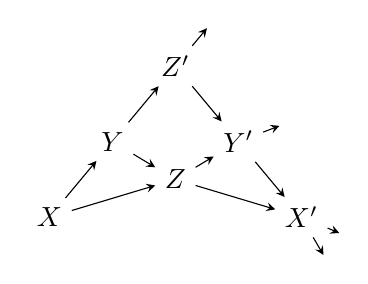
\begin{tikzpicture}[>=stealth,scale=.8]
\node(a)at(0,0){$X$};\node(b)at(1,1.2){$Y$};\node(c)at(2,2.4){$Z'$};\node(d)at(2,.6){$Z$};\node(e)at(3,1.2){$Y'$};\node(f)at(4,0){$X'$};
\draw[->](a)--(b);\draw[->](b)--(c);\draw[->](c)--(e);\draw[->](e)--(f);\draw[->](a)--(d);\draw[->](b)--(d);\draw[->](d)--(e);\draw[->](d)--(f);
\draw[->](c)--++(.5,.6);\draw[->](e)--++(.65,.25);\draw[->](f)--++(.6,-.25);\draw[->](f)--++(.35,-.6);
\end{tikzpicture}
\tag{1.1.7.1}
\end{equation*}
这一画法突出了\term{distinguished-triangle}{区别三角}的态射
\[
 (X,Y,Z')\longrightarrow(X,Z,Y')\longrightarrow(Y,Z,X')\longrightarrow(Z',Y',X'),
\]
只是对每个态射，其中一个相应的交换方形没有明显显示出来。此外，图中的对称性也被打破了，所以补全上述态射链的\term{distinguished-triangle}{区别三角}态射 $(Z',Y',X')\to(Z',X[1],Y[1])$ 没有明显显示出来。

\par\medskip\noindent\textbf{1.1.8.} 可将(1.1.7.1)与如下事实比较：在\term{abelian-category}{阿贝尔范畴}中，两个可复合单态射 $X\to Y\to Z$ 给出由短\term{exact-sequence}{正合列}组成的图
\SourcePage{30}
\begin{equation*}
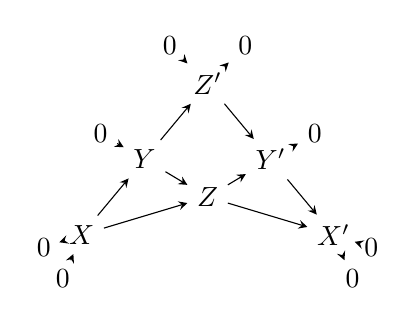
\begin{tikzpicture}[>=stealth,scale=.8]
\node(a)at(0,0){$X$};\node(b)at(1,1.2){$Y$};\node(c)at(2,2.4){$Z'$};\node(d)at(2,.6){$Z$};\node(e)at(3,1.2){$Y'$};\node(f)at(4,0){$X'$};
\draw[->](a)--(b);\draw[->](b)--(c);\draw[->](c)--(e);\draw[->](e)--(f);\draw[->](a)--(d);\draw[->](b)--(d);\draw[->](d)--(e);\draw[->](d)--(f);
\node(z1)at(-.6,-.2){$0$};\draw[->](z1)--(a);\node(z2)at(-.3,-.7){$0$};\draw[->](z2)--(a);
\node(z3)at(.3,1.6){$0$};\draw[->](z3)--(b);\node(z4)at(1.4,3){$0$};\draw[->](z4)--(c);
\node(z5)at(2.6,3){$0$};\draw[->](c)--(z5);\node(z6)at(3.7,1.6){$0$};\draw[->](e)--(z6);
\node(z7)at(4.6,-.2){$0$};\draw[->](f)--(z7);\node(z8)at(4.3,-.7){$0$};\draw[->](f)--(z8);
\end{tikzpicture}\tag{1.1.8.1}
\end{equation*}
它表达的是 $(Z/X)/(Y/X)=Z/Y$。(1.1.7.1)与(1.1.8.1)的关系如下。设在 $A$ 中对象的\term{complex}{复形}所成的\term{abelian-category}{阿贝尔范畴} $C(A)$ 中给定一个图(1.1.8.1)。$C(A)$ 中每个短\term{exact-sequence}{正合列}都定义 $D(A)$ 中的一个\term{distinguished-triangle}{区别三角}（[10] 第31页）；由图(1.1.8.1)的短\term{exact-sequence}{正合列}得到的\term{distinguished-triangle}{区别三角}构成一个八面体(1.1.7.1)。特别地，通过 $A\mapsto(\text{仅在0次为 $A$ 的\term{complex}{复形}})$，将\term{abelian-category}{阿贝尔范畴} $A$ 与 $DA$ 的一个全子范畴等同。于是对 $A$ 中任意短\term{exact-sequence}{正合列} $0\to A\to B\to C\to0$，都存在唯一的从 $C$ 到 $A$ 的一次箭头 $d$，使三角 $A\to B\to C\xrightarrow{d}$ 为\term{distinguished-triangle}{区别三角}。存在性是每个\term{complex}{复形}短\term{exact-sequence}{正合列}都确定\term{distinguished-triangle}{区别三角}（[10] 第31页）的特例；唯一性来自下述1.1.10以及：当 $A,B$ 属于 $A$ 时，$n<0$ 蕴涵 $\Hom^n(A,B)=0$（$n\geq0$ 时，它是 $A$ 被 $B$ \term{extension}{扩张}的第 $n$ 个 Yoneda $\Ext$）。从 $A$ 中的图(1.1.8.1)出发，在 $DA$ 中将其中每个短\term{exact-sequence}{正合列}补成\term{distinguished-triangle}{区别三角}，就得到图(1.1.7.1)。这是 TR 4 的一个推论。

\par\medskip\noindent\textbf{命题1.1.9。} 设 $(X,Y,Z)$ 与 $(X',Y',Z')$ 是两个\term{distinguished-triangle}{区别三角}，$g:Y\to Y'$：
\[
\begin{tikzcd}[ampersand replacement=\&]
X\arrow[r,"{u}"]\arrow[d,dashed,"{f}"']\&Y\arrow[r,"{v}"]\arrow[d,"{g}"]\&Z\arrow[r,"{d}"]\arrow[d,dashed,"{h}"]\&X[1]\\
X'\arrow[r,"{u'}"']\&Y'\arrow[r,"{v'}"']\&Z'\arrow[r,"{d'}"']\&X'[1]
\end{tikzcd}
\]
以下条件\term{equivalence}{等价}：\textup{(a)} $v'gu=0$；\textup{(b)} 存在 $f$ 使第一个方形交换；\textup{(b$'$)} 存在 $h$ 使第二个方形交换；\textup{(c)} 存在三角态射 $(f,g,h)$。若这些条件成立且 $\Hom^{-1}(X,Z')=0$，则 \textup{(b)} 中的 $f$ 和 \textup{(b$'$)} 中的 $h$ 各自唯一。

将\term{exact-sequence}{正合列}
\[
 \Hom^{-1}(X,Z')\longrightarrow\Hom(X,X')\longrightarrow\Hom(X,Y')\longrightarrow\Hom(X,Z')
\]
应用于 $\Hom(X,Y')$ 中的 $gu$，便得 $(a)\Longleftrightarrow(b)$，并且当 $\Hom^{-1}(X,Z')=0$ 时 $f$ 唯一。$(b)\Longrightarrow(c)$ 来自 TR 2：若 $f$ 满足 $(b)$，则存在 $h$ 使
\SourcePage{31}
$(f,g,h)$ 成为三角态射。反向蕴涵显然。最后，\term{duality}{对偶}论证给出 $(a)\Longleftrightarrow(b')$，以及当 $\Hom^{-1}(X,Z')=0$ 时 $h$ 的唯一性。

\par\medskip\noindent\textbf{推论1.1.10。} 设 $X\xrightarrow{u}Y\xrightarrow{v}Z\xrightarrow{d}$ 是\term{distinguished-triangle}{区别三角}。若 $\Hom^{-1}(X,Z)=0$，则
\begin{enumerate}[label=(\roman*)]
\item $u$ 的\term{cone}{锥}在唯一同构意义下唯一；
\item $d$ 是唯一使 $X\xrightarrow{u}Y\xrightarrow{v}Z\xrightarrow{x}$ 为\term{distinguished-triangle}{区别三角}的态射 $x:Z\to X[1]$。
\end{enumerate}
若在1.1.9中取 $X=X'$、$Y=Y'$，并令 $f,g$ 都是恒等态射，则 $Z\simeq Z'$，从而 $\Hom^{-1}(X,Z')=0$；于是(i)来自 $h$ 的唯一性。为证(ii)，将1.1.9应用于
\[
\begin{tikzcd}[ampersand replacement=\&]
X\arrow[r,"{u}"]\arrow[d,equal]\&Y\arrow[r,"{v}"]\arrow[d,equal]\&Z\arrow[r,"{d}"]\arrow[d,dashed,"{h}"]\&X[1]\arrow[d,equal]\\
X\arrow[r,"{u}"']\&Y\arrow[r,"{v}"']\&Z\arrow[r,"{x}"']\&X[1]
\end{tikzcd}
\]
必有 $h=\id_Z$，故 $d=x$。

\term{duality}{对偶}地，在1.1.10的条件下，$v$ 的\term{cone}{锥}在唯一同构意义下唯一。

下面的命题由 J. L. Verdier 告知我们。

\par\medskip\noindent\textbf{命题1.1.11。} 任意交换方形 $(X'Y'XY)$ 都可以补成一个九对象图：
\[
\begin{tikzcd}[ampersand replacement=\&,column sep=small]
X'[1]\arrow[r,dashed]\&Y'[1]\arrow[r,dashed]\&Z'[1]\arrow[r,dashed]\&X'[2]\\
X''\arrow[u,dashed]\arrow[r]\&Y''\arrow[u,dashed]\arrow[r]\&Z''\arrow[u,dashed]\arrow[r]\&X''[1]\arrow[u,dashed]\\
X\arrow[u]\arrow[r]\&Y\arrow[u]\arrow[r]\&Z\arrow[u]\arrow[r]\&X[1]\arrow[u,dashed]\\
X'\arrow[u]\arrow[r]\&Y'\arrow[u]\arrow[r]\&Z'\arrow[u]\arrow[r]\&X'[1]\arrow[u,dashed]
\end{tikzcd}
\]
其中虚线箭头由实线箭头施以\term{shift-functor}{平移函子}得到；各方形交换，唯独右上角的方形反交换；实线的各行、各列都是\term{distinguished-triangle}{区别三角}。

取\term{distinguished-triangle}{区别三角} $(X',Y',Z')$、$(X,Y,Z)$、$(X',X,X'')$、$(Y',Y,Y'')$ 和 $(X',Y,A)$，其底边分别为所给交换方形的四边及其对角线 $X'\to Y$。公理 TR 4 允许我们补全如下两个八面体：
\SourcePage{32}
\begin{center}
\begin{tikzpicture}[>=stealth,scale=.68]
\node(a)at(0,0){$X'$};\node(b)at(1,1.2){$Y'$};\node(c)at(2,2.4){$Z'$};\node(d)at(2,.6){$Y$};\node(e)at(3,1.2){$A$};\node(f)at(4,0){$Y''$};
\draw[->](a)--(b);\draw[->](b)--(c);\draw[->](c)--(e);\draw[->](e)--(f);\draw[->](a)--(d);\draw[->](b)--(d);\draw[->](d)--(e);\draw[->](d)--(f);\draw[->](c)--++(.4,.6);\draw[->](e)--++(.6,.2);\draw[->](f)--++(.5,-.25);\draw[->](f)--++(.3,-.6);
\node at(-.5,1.2){(1)};\node at(2,-.8){基于 $X'\to Y'\to Y$};
\begin{scope}[xshift=6.4cm]
\node(a)at(0,0){$X'$};\node(b)at(1,1.2){$X$};\node(c)at(2,2.4){$X''$};\node(d)at(2,.6){$Y$};\node(e)at(3,1.2){$A$};\node(f)at(4,0){$Z$};
\draw[->](a)--(b);\draw[->](b)--(c);\draw[->](c)--(e);\draw[->](e)--(f);\draw[->](a)--(d);\draw[->](b)--(d);\draw[->](d)--(e);\draw[->](d)--(f);\draw[->](c)--++(.4,.6);\draw[->](e)--++(.6,.2);\draw[->](f)--++(.5,-.25);\draw[->](f)--++(.3,-.6);
\node at(-.5,1.2){(2)};\node at(2,-.8){基于 $X'\to X\to Y$};
\end{scope}
\end{tikzpicture}
\end{center}
再补出八面体
\begin{center}
\begin{tikzpicture}[>=stealth,scale=.7]
\node(a)at(0,0){$X''$};\node(b)at(1,1.2){$A$};\node(c)at(2,2.4){$Z$};\node(d)at(2,.6){$Y''$};\node(e)at(3,1.2){$Z''$};\node(f)at(4,0){$Z'[1]$};
\draw[->](a)--(b);\draw[->](b)--(c);\draw[->](c)--(e);\draw[->](e)--(f);\draw[->](a)--(d);\draw[->](b)--(d);\draw[->](d)--(e);\draw[->](d)--(f);\draw[->](c)--++(.4,.6);\draw[->](e)--++(.6,.2);\draw[->](f)--++(.5,-.25);\draw[->](f)--++(.3,-.6);
\node at(-.6,1.2){(3)};\node at(2,-.8){基于 $X''\to A\to Y''$};
\end{tikzpicture}
\end{center}
其中的\term{distinguished-triangle}{区别三角} $(A,Y'',Z'[1])$ 由(1)中的 $(Z',A,Y'')$ 旋转而得：将箭头 $Z'\to A$ 改变符号。

所需的\term{distinguished-triangle}{区别三角}都出现在这些八面体中，只有 $(Z',Z,Z'')$ 以 $(Z,Z'',Z'[1])$ 的形式出现；将箭头 $Z'\to Z$ 改变符号，就可由 $(Z,Z'',Z'[1])$ 得到 $(Z',Z,Z'')$。

为证明所需的交换性与反交换性，注意从 $X',Y',Z'$ 到 $X,Y,Z$ 的箭头组成如下三角态射的复合：
\[
 (X',Y',Z')\xrightarrow{(1)}(X',Y,A)\xrightarrow{(2)}(X,Y,Z),
\]
这些态射出现在(1)与(2)中；从 $X,Y,Z$ 到 $X'',Y'',Z''$ 的箭头组成如下三角态射的复合：
\[
 (X,Y,Z)\xrightarrow{(2)}(X'',A,Z)\xrightarrow{(3)}(X'',Y'',Z'');
\]
而从 $X'',Y'',Z''$ 到 $X'[1],Y'[1],Z'[1]$ 的箭头组成如下三角态射的复合：
\[
 (X'',Y'',Z'')\xrightarrow{(3)}(A,Y'',Z'[1])\xrightarrow{(1)}(X'[1],Y'[1],Z'[1]),
\]
最后一个箭头由(1)中的三角态射 $(Z',A,Y'')\to(Z',X'[1],Y'[1])$ 旋转而来。在\term{distinguished-triangle}{区别三角} $(X'[1],Y'[1],Z'[1])$ 中，一次箭头与三角 $(X',Y',Z')$ 的一次箭头的平移相差一个符号；这就解释了第九个方形的反交换性。

\par\medskip\noindent\textbf{注1.1.12。} 一个由\term{complex}{复形}\term{exact-sequence}{正合列}组成的方形，在\term{derived-category}{导出范畴}中定义一个九对象图。第九个方形的反交换性精确说明了相应连接同态的反交换性。

\par\medskip\noindent\textbf{注1.1.13。} 在通常的\term{triangulated-category}{三角范畴}中（$A$ 加性时的 $KA$，$A$ 正合时的 $DA$，稳定\term{homotopy}{同伦}范畴等），每个“八面体上半部”形式的图都能补成一个八面体，
\SourcePage{33}
使下列三角为\term{distinguished-triangle}{区别三角}：
\[
 Y\longrightarrow Y'\longrightarrow X'\oplus X[1]\xrightarrow{(1)}Y,
 \qquad
 Y\longrightarrow Z\oplus Z'\longrightarrow Y'\xrightarrow{(1)}Y
\]
（箭头取自八面体，唯独第一式中的 $Y'\to X[1]$、第二式中的 $Z'\to Y'$ 分别与八面体中的箭头反号）。一般情况下是否如此，我们并不清楚。如果这些三角今后有用，或许应该加强\term{triangulated-category}{三角范畴}的公理 TR 4，重新定义“八面体”，将上述三角为\term{distinguished-triangle}{区别三角}纳入八面体的定义。

\par\medskip\noindent\textbf{注1.1.14。} 三角图与八面体图有如下推广；它们分别是 $N=3$ 与 $N=4$ 的特例。对 $N\geq2$，一个这样的图包含以下数据：
\begin{enumerate}[label=(\alph*)]
\item 对 $\Z$ 的每个满足 $0<\#I<N$ 的区间 $I$，给定对象 $K(I)$。
\item 若 $I=[a,b[$、$J=[c,d[$，定义 $I\leq J\Longleftrightarrow(a\leq c\text{ 且 }b\leq d)$。对 $I\leq J$ 给定箭头 $\varphi_{JI}:K(I)\to K(J)$，满足 $\varphi_{KJ}\varphi_{JI}=\varphi_{KI}$ 及 $\varphi_{II}=\id$。若 $I=[a,b[$、$J=[c,d[$ 且 $b\leq c$，则要求 $\varphi_{JI}=0$。
\item 对 $I=[a,b[$ 定义 $I^*=[b,a+N[$。给定同构 $K(I^*)=K(I)[1]$，对 $I\leq J$，使图
\[
\begin{tikzcd}[ampersand replacement=\&]
 K(I)[1]\arrow[r,equal]\arrow[d,"{\varphi_{JI}[1]}"']\&K(I^*)\arrow[d,"{\varphi_{J^*I^*}}"]\\
 K(J)[1]\arrow[r,equal]\&K(J^*)
\end{tikzcd}
\]
交换。
\item 对 $a<b<c<a+N$，由箭头 $\varphi$ 组成的三角
\[
 K([a,b[)\longrightarrow K([a,c[)\longrightarrow K([b,c[)\longrightarrow K([b,a+N[)=K([a,b[)[1]
\]
为\term{distinguished-triangle}{区别三角}。
\end{enumerate}
一个具有 $N-1$ 阶\term{filtration}{滤过}、且\term{filtration}{滤过}逐次可裂的\term{complex}{复形}，在 $KA$ 中定义这样的图。若 $K$ 的\term{filtration}{滤过} $W$ 取为递增\term{filtration}{滤过}，$W_0K=0$ 且 $W_{N-1}K=K$（即 $i\notin[1,N-1]$ 时 $\mathrm{Gr}^W_iK=0$），那么对 $1\leq a<b\leq N$ 有 $K([a,b[)=W_{b-1}K/W_{a-1}K$，并且 $K(\{0\})=K[-1]$。
\SourcePage{34}
\section*{1.2. 阿贝尔子范畴}
\addcontentsline{toc}{section}{1.2. 阿贝尔子范畴}
\par\medskip\noindent\textbf{1.2.0.} 设 $\mathcal D$ 是\term{triangulated-category}{三角范畴}，$\mathcal C$ 是 $\mathcal D$ 的全子范畴。我们假设，当 $i<0$ 且 $X,Y\in\mathcal C$ 时，$\Hom^i(X,Y):=\Hom(X,Y[i])=0$。

\par\medskip\noindent\textbf{例1.2.1。} $\mathcal D$ 是\term{abelian-category}{阿贝尔范畴} $A$ 的\term{derived-category}{导出范畴}，$\mathcal C=A$，并通过函子 $A\mapsto(\text{仅在0次为 $A$ 的\term{complex}{复形}})$ 将它与 $\mathcal D$ 的全子范畴等同。

\par\medskip\noindent\textbf{命题1.2.2。} 设 $f:X\to Y$ 是 $\mathcal C$ 中的态射。将 $f$ 补成\term{distinguished-triangle}{区别三角} $X\to Y\to S\to$，并假设 $S$ 属于一个\term{distinguished-triangle}{区别三角} $N[1]\to S\to C\to$，其中 $N,C\in\mathcal C$：
\begin{equation*}
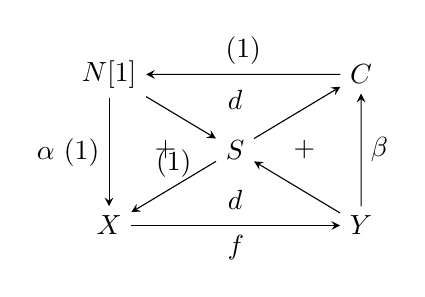
\begin{tikzpicture}[>=stealth,scale=.8]
\node(a)at(0,2.4){$N[1]$};\node(b)at(4,2.4){$C$};\node(c)at(0,0){$X$};\node(d)at(4,0){$Y$};\node(e)at(2,1.2){$S$};
\draw[->](b)--node[above]{$(1)$}(a);\draw[->](a)--node[left]{$\alpha\ (1)$}(c);\draw[->](c)--node[below]{$f$}(d);\draw[->](d)--node[right]{$\beta$}(b);
\draw[->](a)--(e);\draw[->](e)--(b);\draw[->](e)--node[above]{$(1)$}(c);\draw[->](d)--(e);
\node at(2,2){$d$};\node at(.9,1.2){$+$};\node at(3.1,1.2){$+$};\node at(2,.4){$d$};
\end{tikzpicture}\tag{1.2.2.1}
\end{equation*}
标有 $+$ 的三角交换，标有 $d$ 的三角为\term{distinguished-triangle}{区别三角}。则 $\alpha[-1]:N\to X$ 是 $f$ 在 $\mathcal C$ 中的核，$\beta:Y\to C$ 是其余核。

对 $Z\in\mathcal C$，由 $\Hom$ 的长\term{exact-sequence}{正合列}和1.2.0，得到\term{exact-sequence}{正合列}
\[
 \begin{gathered}
 0\to\Hom^{-1}(Z,S)\to\Hom(Z,X)\to\Hom(Z,Y),\\[3pt]
 0\to\Hom(Z,N)\to\Hom^{-1}(Z,S)\to0.
 \end{gathered}
\]
这说明 $(N,\alpha[-1])$ 是 $f$ 的核。\term{duality}{对偶}论证表明 $(C,\beta)$ 是余核。

\par\medskip\noindent\textbf{例。} 对 $A\subset D(A)$（例1.2.1），$f:X\to Y$ 的\term{cone}{锥} $S$ 是\term{complex}{复形} $X\xrightarrow{f}Y$（$X$ 在 $-1$ 次，$Y$ 在0次）。它有子\term{complex}{复形} $\Ker(f)[1]=H^{-1}(S)[1]$，而商\term{complex}{复形} $X/\Ker(f)\to Y$ \term{quasi-isomorphism}{拟同构}地映到置于0次的 $\Coker(f)=H^0(S)$。因此得到图(1.2.2.1)。

\par\medskip\noindent\textbf{1.2.3.} 若 $\mathcal C$ 中的态射 $f:X\to Y$ 是某个图(1.2.2.1)的底边，则称它为 $\mathcal C$-\term{admissible}{容许}态射；当 $\mathcal C$ 不致混淆时，简称\term{admissible}{容许}态射。若 $f$ 是单态射，由1.2.2得 $N=0$，从而 $S\simeq C$，(1.2.2.1)退化为\term{distinguished-triangle}{区别三角} $(X,Y,C)$。若 $f$ 是满态射，则 $C=0$，从而 $N[1]\simeq S$，(1.2.2.1)退化为\term{distinguished-triangle}{区别三角} $(N,X,Y)$。反之，对任意\term{distinguished-triangle}{区别三角} $X\xrightarrow{f}Y\xrightarrow{g}Z\xrightarrow{d}$，
\SourcePage{35}
若 $X,Y,Z\in\mathcal C$，则 $f,g$ 均\term{admissible}{容许}，$f$ 是 $g$ 的核，$g$ 是 $f$ 的余核。由1.2.0及1.1.10，$d$ 由 $f,g$ 确定。

若 $\mathcal C$ 中的列 $X\to Y\to Z$ 可由某个\term{distinguished-triangle}{区别三角}去掉一次箭头得到，则称它为\term{admissible}{容许}短\term{exact-sequence}{正合列}。

\par\medskip\noindent\textbf{命题1.2.4。} 假设 $\mathcal C$ 对有限直和封闭。以下条件\term{equivalence}{等价}：
\begin{enumerate}[label=(\roman*)]
\item $\mathcal C$ 是\term{abelian-category}{阿贝尔范畴}，且它的短\term{exact-sequence}{正合列}均\term{admissible}{容许}；
\item $\mathcal C$ 的每个态射都是 $\mathcal C$-\term{admissible}{容许}态射。
\end{enumerate}
证明 $(ii)\Longrightarrow(i)$。由1.2.2，$\mathcal C$ 的每个态射都有核与余核；要证 $\mathcal C$ 是\term{abelian-category}{阿贝尔范畴}，只须再验证 $\mathrm{Coim}(f)\simeq\im(f)$。将(1.2.2.1)看作八面体的下半部，应用 TR $4'$（见1.1.7）补成八面体：
\begin{center}
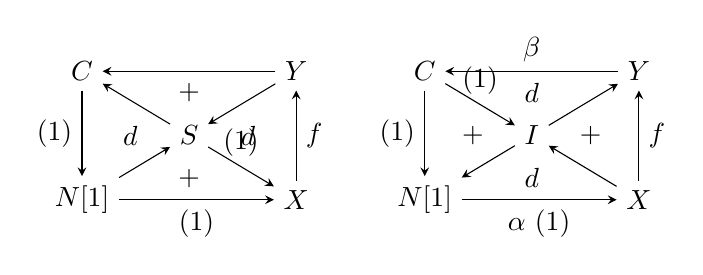
\begin{tikzpicture}[>=stealth,scale=.68]
\node(a)at(0,2.4){$C$};\node(b)at(4,2.4){$Y$};\node(c)at(0,0){$N[1]$};\node(d)at(4,0){$X$};\node(e)at(2,1.2){$S$};
\draw[->](b)--(a);\draw[->](a)--node[left]{$(1)$}(c);\draw[->](c)--node[below]{$(1)$}(d);\draw[->](d)--node[right]{$f$}(b);\draw[->](e)--(a);\draw[->](b)--(e);\draw[->](c)--(e);\draw[->](e)--node[above]{$(1)$}(d);\node at(2,2){$+$};\node at(.9,1.2){$d$};\node at(3.1,1.2){$d$};\node at(2,.4){$+$};
\begin{scope}[xshift=6.4cm]
\node(a)at(0,2.4){$C$};\node(b)at(4,2.4){$Y$};\node(c)at(0,0){$N[1]$};\node(d)at(4,0){$X$};\node(e)at(2,1.2){$I$};
\draw[->](b)--node[above]{$\beta$}(a);\draw[->](a)--node[left]{$(1)$}(c);\draw[->](c)--node[below]{$\alpha\ (1)$}(d);\draw[->](d)--node[right]{$f$}(b);\draw[->](a)--node[above]{$(1)$}(e);\draw[->](e)--(b);\draw[->](e)--(c);\draw[->](d)--(e);\node at(2,2){$d$};\node at(.9,1.2){$+$};\node at(3.1,1.2){$+$};\node at(2,.4){$d$};
\end{scope}
\end{tikzpicture}
\end{center}
由1.2.2，$\beta$ 作为 $f$ 的余核，是满态射。由1.2.3及\term{distinguished-triangle}{区别三角} $(I,Y,C)$，知 $I\in\mathcal C$ 且 $I$ 是 $f$ 的像。\term{duality}{对偶}地，将上半部的另一个\term{distinguished-triangle}{区别三角}旋转所得的\term{distinguished-triangle}{区别三角} $(N,X,I)$ 表明，$I$ 是 $f$ 的余像。最后，由1.2.3，$\mathcal C$ 的短\term{exact-sequence}{正合列}均\term{admissible}{容许}。

证明 $(i)\Longrightarrow(ii)$。$f:X\to Y$ 的核 $N$、余核 $C$ 和像 $I$ 给出两个短\term{exact-sequence}{正合列} $0\to N\to X\to I\to0$ 与 $0\to I\to Y\to C\to0$，因而给出组成上述上半部图的两个三角。应用 TR 4，便得到下半部，即 $f$ \term{admissible}{容许}。

\par\medskip\noindent\textbf{定义1.2.5。} $\mathcal D$ 的全子范畴 $\mathcal C$ 若满足1.2.0及1.2.4的\term{equivalence}{等价}条件，则称为\term{admissible}{容许}\term{abelian-subcategory}{阿贝尔子范畴}。

\par\medskip\noindent\textbf{1.2.6.} 在\term{triangulated-category}{三角范畴} $\mathcal D$ 中，若存在\term{distinguished-triangle}{区别三角} $(X,Y,Z)$，有时称对象 $Y$ 是 $Z$ 被 $X$ 的\term{extension}{扩张}。若对每个满足 $X,Z\in\mathcal D'$ 的\term{distinguished-triangle}{区别三角} $(X,Y,Z)$ 都有 $Y\in\mathcal D'$，则称 $\mathcal D$ 的子范畴 $\mathcal D'$ 对\term{extension}{扩张}封闭。

\SourcePage{36}
\section*{1.3. $t$-范畴}
\addcontentsline{toc}{section}{1.3. $t$-范畴}
\par\medskip\noindent\textbf{定义1.3.1。} 一个 $t$-范畴是\term{triangulated-category}{三角范畴} $\mathcal D$，配备两个严格全子范畴 $\mathcal D^{\leq0}$ 与 $\mathcal D^{\geq0}$，使得置 $\mathcal D^{\leq n}:=\mathcal D^{\leq0}[-n]$、$\mathcal D^{\geq n}:=\mathcal D^{\geq0}[-n]$ 后，有：
\begin{enumerate}[label=(\roman*)]
\item 当 $X\in\mathcal D^{\leq0}$、$Y\in\mathcal D^{\geq1}$ 时，$\Hom(X,Y)=0$；
\item $\mathcal D^{\leq0}\subset\mathcal D^{\leq1}$ 且 $\mathcal D^{\geq0}\supset\mathcal D^{\geq1}$；
\item 对任意 $X\in\mathcal D$，存在\term{distinguished-triangle}{区别三角} $(A,X,B)$，其中 $A\in\mathcal D^{\leq0}$、$B\in\mathcal D^{\geq1}$。
\end{enumerate}
也称 $(\mathcal D^{\leq0},\mathcal D^{\geq0})$ 为 $\mathcal D$ 上的一个\term{t-structure}{$t$-结构}。它的\term{heart}{心}是全子范畴 $\mathcal C:=\mathcal D^{\leq0}\cap\mathcal D^{\geq0}$。

\par\medskip\noindent\textbf{例1.3.2。} (i) 设 $A$ 是\term{abelian-category}{阿贝尔范畴}。$DA$ 的自然 \term{t-structure}{$t$-结构}定义为：$(DA)^{\leq n}$（相应地，$(DA)^{\geq n}$）是满足 $i>n$（相应地，$i<n$）时 $H^iK=0$ 的\term{complex}{复形} $K$ 所成的子范畴；也就是说，$K$ \term{quasi-isomorphism}{拟同构}于在次数 $>n$（相应地，$<n$）为零的\term{complex}{复形} $K'$。来验证1.3.1(iii)。对每个\term{complex}{复形} $K$，其\term{truncation}{截断} $\tau_{\leq0}K$ 是 $K$ 的子\term{complex}{复形} $\cdots\to K^{-1}\to\Ker(d^0)\to0\to\cdots$。须注意，[7] 将该\term{truncation}{截断}记为 $\sigma_{\leq0}K$，[8] 则记为 $t_{0]}$。置 $\tau_{\geq1}K:=K/\tau_{\leq0}K$，则 $\tau_{\leq0}K\in(DA)^{\leq0}$、$\tau_{\geq1}K\in(DA)^{\geq1}$；短\term{exact-sequence}{正合列} $0\to\tau_{\leq0}K\to K\to\tau_{\geq1}K\to0$ 给出所需的三角。1.3.1(i)、(ii)的验证留给读者。

(ii) 若 $(\mathcal D^{\leq0},\mathcal D^{\geq0})$ 是 $\mathcal D$ 上的 \term{t-structure}{$t$-结构}，则对任意整数 $n$，$(\mathcal D^{\leq n},\mathcal D^{\geq n})$ 也是一个 \term{t-structure}{$t$-结构}，称其由原 \term{t-structure}{$t$-结构}经平移得到。

(iii) 若 $(\mathcal D^{\leq0},\mathcal D^{\geq0})$ 是 $\mathcal D$ 上的 \term{t-structure}{$t$-结构}，则 $((\mathcal D^{\geq0})^{\mathrm{opp}},(\mathcal D^{\leq0})^{\mathrm{opp}})$ 是\term{duality}{对偶}\term{triangulated-category}{三角范畴} $\mathcal D^{\mathrm{opp}}$ 上的 \term{t-structure}{$t$-结构}，称为\term{duality}{对偶} \term{t-structure}{$t$-结构}。这使我们可以使用\term{duality}{对偶}论证（若将一个命题应用于\term{duality}{对偶} $t$-范畴得到另一个命题，就称二者\term{duality}{对偶}）。

以下设 $\mathcal D$ 是一个 $t$-范畴。

\par\medskip\noindent\textbf{命题1.3.3。} (i) 包含函子 $\mathcal D^{\leq n}\hookrightarrow\mathcal D$ 有右\term{adjunction}{伴随} $\tau_{\leq n}$，而 $\mathcal D^{\geq n}\hookrightarrow\mathcal D$ 有左\term{adjunction}{伴随} $\tau_{\geq n}$。

(ii) 对任意 $X\in\mathcal D$，存在唯一的态射 $d\in\Hom^1(\tau_{\geq1}X,\tau_{\leq0}X)$，使三角
\[
 \tau_{\leq0}X\longrightarrow X\longrightarrow\tau_{\geq1}X\xrightarrow{d}
\]
\SourcePage{37}
为\term{distinguished-triangle}{区别三角}。在唯一同构意义下，它是唯一满足 $A\in\mathcal D^{\leq0}$、$B\in\mathcal D^{\geq1}$ 的\term{distinguished-triangle}{区别三角} $(A,X,B)$。

由\term{duality}{对偶}性和平移，只须对 $\mathcal D^{\leq0}$ 验证(i)。也就是对每个 $X\in\mathcal D$，寻找 $A\in\mathcal D^{\leq0}$ 及箭头 $A\to X$（即 $\tau_{\leq0}$ 在 $X$ 处的值），使对任意 $T\in\mathcal D^{\leq0}$ 都有 $\Hom(T,A)\xrightarrow{\sim}\Hom(T,X)$。取1.3.1(iii)中的三角 $(A,X,B)$。$\Hom$ 的长\term{exact-sequence}{正合列}和条件1.3.1(i)、(ii)给出 $\Hom(T,A)\xrightarrow{\sim}\Hom(T,X)$，因此 $A=\tau_{\leq0}X$。这证明了(i)，也证明了\term{distinguished-triangle}{区别三角} $(\tau_{\leq0}X,X,\tau_{\geq1}X)$ 的存在性，以及：忘掉一次箭头后，1.3.1(iii)中的每个\term{distinguished-triangle}{区别三角} $(A,X,B)$ 都与此三角唯一同构。一次箭头的唯一性由1.3.1(i)、(ii)及1.1.10(ii)得到。

\par\medskip\noindent\textbf{1.3.4.} \term{distinguished-triangle}{区别三角} $(\tau_{\leq0}X,X,\tau_{\geq1}X)$ 表明下列条件\term{equivalence}{等价}：
\begin{align*}
 (a)\;&\tau_{\leq0}X=0,
 & (a')\;&\text{对每个 $T\in\mathcal D^{\leq0}$，$\Hom(T,X)=0$};\\
 (b)\;&X\xrightarrow{\sim}\tau_{\geq1}X,
 & (b')\;&X\in\mathcal D^{\geq1}.
\end{align*}
\term{equivalence}{等价}关系 $(a')\Longleftrightarrow(b')$ 可表述为：$\mathcal D^{\geq1}$ 是 $\mathcal D^{\leq0}$ 的右正交。由此可见，$\mathcal D^{\geq1}$ 对\term{extension}{扩张}封闭（1.2.6）。\term{duality}{对偶}地，$\tau_{\geq1}X=0$ 当且仅当 $X\in\mathcal D^{\leq0}$；$\mathcal D^{\leq0}$ 是 $\mathcal D^{\geq1}$ 的左正交，并对\term{extension}{扩张}封闭。特别地，$\mathcal D^{\leq0}$ 与 $\mathcal D^{\geq1}$ 都对有限直和封闭。

对 $a\leq b$，有 $\mathcal D^{\leq a}\subset\mathcal D^{\leq b}$，故存在唯一的态射 $\tau_{\leq a}X\to\tau_{\leq b}X$，使图
\[
\begin{tikzcd}[ampersand replacement=\&]
\tau_{\leq a}X\arrow[rr]\arrow[dr]\&\&\tau_{\leq b}X\arrow[dl]\\
\&X\&
\end{tikzcd}
\]
交换。它将 $\tau_{\leq a}X$ 与 $\tau_{\leq a}\tau_{\leq b}X$ 等同。\term{duality}{对偶}地，有态射 $\tau_{\geq a}X\to\tau_{\geq b}X$，将 $\tau_{\geq b}X$ 与 $\tau_{\geq b}\tau_{\geq a}X$ 等同。

对任意整数 $a$，记 $\tau_{>a}:=\tau_{\geq a+1}$、$\tau_{<a}:=\tau_{\leq a-1}$。由本段第一段平移可知，$X\in\mathcal D^{\leq a}$ \term{equivalence}{等价}于 $\tau_{>a}X=0$。设 $X\in\mathcal D^{\leq a}$。若 $b>a$，则 $\tau_{\geq b}X=0$；若 $b\leq a$，则 $\tau_{>a}\tau_{\geq b}X=\tau_{>a}X=0$。因此 $\tau_{\geq b}$ 将 $\mathcal D^{\leq a}$ 映入自身。

\par\medskip\noindent\textbf{命题1.3.5。} 设 $a\leq b$。对任意 $X\in\mathcal D$，存在唯一态射 $\tau_{\geq a}\tau_{\leq b}X\to\tau_{\leq b}\tau_{\geq a}X$，使图
\SourcePage{38}
\[
\begin{tikzcd}[ampersand replacement=\&]
 \tau_{\leq b}X\arrow[r]\arrow[d]\&X\arrow[r]\&\tau_{\geq a}X\\
 \tau_{\geq a}\tau_{\leq b}X\arrow[rr]\&\&\tau_{\leq b}\tau_{\geq a}X\arrow[u]
\end{tikzcd}
\]
交换。此态射是同构。

从 $\tau_{\leq b}X$ 到 $\tau_{\geq a}X\in\mathcal D^{\geq a}$ 的箭头唯一地经 $\tau_{\geq a}\tau_{\leq b}X$ 分解。因为 $\tau_{\geq a}\tau_{\leq b}X\in\mathcal D^{\leq b}$，该箭头又唯一地经 $\tau_{\leq b}\tau_{\geq a}X$ 分解。将 TR 4 应用于 $\tau_{<a}X\to\tau_{\leq b}X\to X$，得到八面体
\begin{equation*}
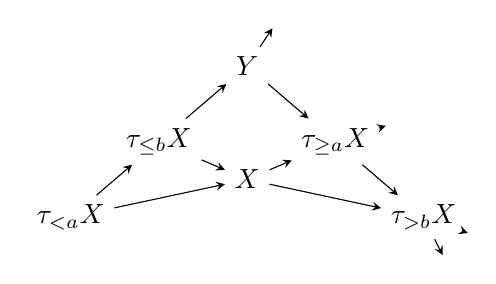
\begin{tikzpicture}[>=stealth,scale=.8]
\node(a)at(0,0){$\tau_{<a}X$};\node(b)at(1.4,1.2){$\tau_{\leq b}X$};\node(c)at(2.8,2.4){$Y$};\node(d)at(2.8,.6){$X$};\node(e)at(4.2,1.2){$\tau_{\geq a}X$};\node(f)at(5.6,0){$\tau_{>b}X$};
\draw[->](a)--(b);\draw[->](b)--(c);\draw[->](c)--(e);\draw[->](e)--(f);\draw[->](a)--(d);\draw[->](b)--(d);\draw[->](d)--(e);\draw[->](d)--(f);\draw[->](c)--++(.4,.6);\draw[->](e)--++(.8,.25);\draw[->](f)--++(.7,-.25);\draw[->](f)--++(.3,-.6);
\end{tikzpicture}\tag{1.3.5.1}
\end{equation*}
在这个八面体中，$Y$ 一方面是 $\tau_{\geq a}\tau_{\leq b}X$，这是因为\term{distinguished-triangle}{区别三角} $(\tau_{<a}X,\tau_{\leq b}X,Y)$ 中有 $\tau_{<a}X=\tau_{<a}\tau_{\leq b}X$；另一方面又是 $\tau_{\leq b}\tau_{\geq a}X$，这是因为有\term{distinguished-triangle}{区别三角} $(Y,\tau_{\geq a}X,\tau_{>b}X)$。

约定 $\tau_{[a,b]}X:=\tau_{\geq a}\tau_{\leq b}X\xrightarrow{\sim}\tau_{\leq b}\tau_{\geq a}X$。

\par\medskip\noindent\textbf{定理1.3.6。} $t$-范畴 $\mathcal D$ 的\term{heart}{心} $\mathcal C:=\mathcal D^{\leq0}\cap\mathcal D^{\geq0}$ 是 $\mathcal D$ 的\term{admissible}{容许}\term{abelian-subcategory}{阿贝尔子范畴}，并对\term{extension}{扩张}封闭（1.2.5、1.2.6）。函子 $H^0:=\tau_{\geq0}\tau_{\leq0}:\mathcal D\to\mathcal C$ 是\term{cohomological-functor}{上同调函子}。

\par\medskip\noindent\textbf{例。} 在1.3.2(i)的情形，$\mathcal C$ 是由与 $A$ 的某个对象同构的 $\mathcal D$ 中对象组成的范畴（这里使用 $A$ 到 $DA$ 的自然嵌入），$H^0$ 与通常的 $H^0$ 函子等同。

\par\medskip\noindent\textbf{证明。} 设 $X,Y\in\mathcal C$，$f:X\to Y$ 的\term{cone}{锥}为 $S$。\term{distinguished-triangle}{区别三角} $(Y,S,X[1])$ 表明 $S\in\mathcal D^{\leq0}\cap\mathcal D^{\geq-1}$。故\term{truncation}{截断} $\tau_{\geq0}S$ 与 $\tau_{\leq-1}S$ 分别属于 $\mathcal C$ 与 $\mathcal C[1]$；\term{distinguished-triangle}{区别三角} $(\tau_{\leq-1}S,S,\tau_{\geq0}S)$ 给出图(1.2.2.1)。这证明 $\mathcal C$ 是\term{admissible}{容许}\term{abelian-subcategory}{阿贝尔子范畴}。$\mathcal C$ 对\term{extension}{扩张}封闭由1.3.4得到。

还须证明：对每个\term{distinguished-triangle}{区别三角} $(X,Y,Z)$，列 $H^0X\to H^0Y\to H^0Z$ 正合。
\SourcePage{39}
\noindent\textbf{情形1。} 若 $X,Y,Z\in\mathcal D^{\leq0}$，则列 $H^0X\to H^0Y\to H^0Z\to0$ 正合。

对 $U\in\mathcal D^{\leq0}$、$V\in\mathcal D^{\geq0}$，有 $H^0U=\tau_{\geq0}U$、$H^0V=\tau_{\leq0}V$，以及
\[
 \Hom(H^0U,H^0V)\xrightarrow{\sim}\Hom(U,H^0V)\xrightarrow{\sim}\Hom(U,V).
\]
对 $T\in\mathcal C$（故 $T\in\mathcal D^{\geq0}$），$\Hom$ 的长\term{exact-sequence}{正合列}给出
\[
 0\to\Hom(Z,T)\to\Hom(Y,T)\to\Hom(X,T),
\]
即 $0\to\Hom(H^0Z,T)\to\Hom(H^0Y,T)\to\Hom(H^0X,T)$。这对每个 $T$ 都成立，因而得到所需正合性。

\noindent\textbf{情形2。} 若 $X\in\mathcal D^{\leq0}$，则列 $H^0X\to H^0Y\to H^0Z\to0$ 正合。

对 $T\in\mathcal D^{\geq1}$，$\Hom$ 的长\term{exact-sequence}{正合列}给出 $\Hom(Z,T)\xrightarrow{\sim}\Hom(Y,T)$，因此 $\tau_{\geq1}Y\xrightarrow{\sim}\tau_{\geq1}Z$。将 TR $4'$（见1.1.7）应用于 $Y\to Z\to\tau_{\geq1}Z$（也可以将 TR 4 应用于 $X\to\tau_{\leq0}Y\to Y$）：
\begin{center}
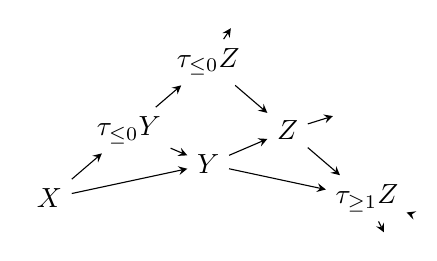
\begin{tikzpicture}[>=stealth,scale=.72]
\node(a)at(0,0){$X$};\node(b)at(1.4,1.2){$\tau_{\leq0}Y$};\node(c)at(2.8,2.4){$\tau_{\leq0}Z$};\node(d)at(2.8,.6){$Y$};\node(e)at(4.2,1.2){$Z$};\node(f)at(5.6,0){$\tau_{\geq1}Z$};
\draw[->](a)--(b);\draw[->](b)--(c);\draw[->](c)--(e);\draw[->](e)--(f);\draw[->](a)--(d);\draw[->](b)--(d);\draw[->](d)--(e);\draw[->](d)--(f);\draw[->](c)--++(.4,.6);\draw[->](e)--++(.8,.25);\draw[->](f)--++(.7,-.25);\draw[->](f)--++(.3,-.6);
\end{tikzpicture}
\end{center}
便得到\term{distinguished-triangle}{区别三角} $(X,\tau_{\leq0}Y,\tau_{\leq0}Z)$，可应用情形1。

\noindent\textbf{情形 $2^*$。} \term{duality}{对偶}地，若 $Z\in\mathcal D^{\geq0}$，则列 $0\to H^0X\to H^0Y\to H^0Z$ 正合。

\noindent\textbf{一般情形。} TR 4 给出八面体
\begin{center}
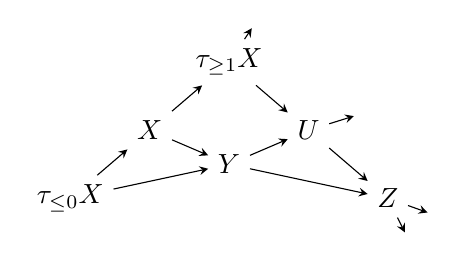
\begin{tikzpicture}[>=stealth,scale=.72]
\node(a)at(0,0){$\tau_{\leq0}X$};\node(b)at(1.4,1.2){$X$};\node(c)at(2.8,2.4){$\tau_{\geq1}X$};\node(d)at(2.8,.6){$Y$};\node(e)at(4.2,1.2){$U$};\node(f)at(5.6,0){$Z$};
\draw[->](a)--(b);\draw[->](b)--(c);\draw[->](c)--(e);\draw[->](e)--(f);\draw[->](a)--(d);\draw[->](b)--(d);\draw[->](d)--(e);\draw[->](d)--(f);\draw[->](c)--++(.4,.6);\draw[->](e)--++(.8,.25);\draw[->](f)--++(.7,-.25);\draw[->](f)--++(.3,-.6);
\end{tikzpicture}
\end{center}
将情形2应用于 $(\tau_{\leq0}X,Y,U)$，得到\term{exact-sequence}{正合列} $H^0X\to H^0Y\to H^0U\to0$；将情形 $2^*$ 应用于 $(U,Z,(\tau_{\geq1}X)[1])$，得到 $0\to H^0U\to H^0Z$。由此可得 $H^0X\to H^0Y\to H^0Z$ 正合。

若 $\bigcap_n\mathcal D^{\leq n}$ 与 $\bigcap_n\mathcal D^{\geq n}$ 都只含零对象，则称该 \term{t-structure}{$t$-结构}\term{nondegenerate}{非退化}。置 $H^iX:=H^0(X[i])$。

\par\medskip\noindent\textbf{命题1.3.7。} 若 $\mathcal D$ 的 \term{t-structure}{$t$-结构}\term{nondegenerate}{非退化}，则函子族 $H^i$ 是\term{conservative}{保守}的；而且，对 $X\in\mathcal D$，
\SourcePage{40}
$X\in\mathcal D^{\leq0}$（相应地，$X\in\mathcal D^{\geq0}$）当且仅当 $i>0$（相应地，$i<0$）时 $H^iX=0$。

设 $X\in\mathcal D$。先证明：若所有 $H^iX$ 都为零，则 $X=0$。若 $X\in\mathcal D^{\leq0}$，则 $H^0X=0$ 保证 $X\in\mathcal D^{\leq-1}$；继续下去可知 $X\in\bigcap_n\mathcal D^{\leq n}$，所以 $X=0$。\term{duality}{对偶}地，若 $X\in\mathcal D^{\geq0}$，同样有 $X=0$。一般情况下，$\tau_{\leq0}X$ 与 $\tau_{\geq1}X$ 的所有 $H^i$ 仍为零，故二者均为零；由\term{distinguished-triangle}{区别三角} $(\tau_{\leq0}X,X,\tau_{\geq1}X)$ 即得结论。

若\term{cone}{锥}为 $Z$ 的态射 $f:X\to Y$ 诱导同构 $H^i(X)\xrightarrow{\sim}H^i(Y)$，则\term{cohomology}{上同调}长\term{exact-sequence}{正合列}表明所有 $H^i(Z)$ 都为零。因此 $Z=0$，$f$ 是同构。最后，若 $i>0$ 时 $H^i(X)=0$，则所有 $H^i(\tau_{>0}X)$ 都为零，故 $\tau_{>0}X=0$，由1.3.4知 $X\in\mathcal D^{\leq0}$。$\mathcal D^{\geq0}$ 的结论由\term{duality}{对偶}性得到。

\par\medskip\noindent\textbf{1.3.8.} 定理1.3.6将 $\mathcal D$ 的每个 \term{t-structure}{$t$-结构}对应于一个\term{admissible}{容许}\term{abelian-subcategory}{阿贝尔子范畴} $\mathcal C$；它有一个逆命题，表述如下（1.3.9）。其证明将持续到1.3.14。本文后续部分不会使用这个结果。

\par\medskip\noindent\textbf{1.3.9.} 设 $\mathcal D$ 是\term{triangulated-category}{三角范畴}，$\operatorname{Isom}(\mathcal D)$ 是其对象的同构类集合，$X\in\mathcal D$ 的同构类记为 $[X]$。以 $*$ 表示如下运算，将 $\operatorname{Isom}(\mathcal D)$ 的两个子集对应于第三个子集：
\[
 A*B=\{[X]\mid\text{存在\term{distinguished-triangle}{区别三角} $(U,X,V)$，其中 $[U]\in A$、$[V]\in B$}\}.
\]
\par\medskip\noindent\textbf{引理1.3.10。} 运算 $*$ 满足结合律。

\noindent\textbf{证明。} 只须证明，对 $X,Y,Z\in\mathcal D$ 有
\[
 (\{[X]\}*\{[Y]\})*\{[Z]\}=\{[X]\}*(\{[Y]\}*\{[Z]\}).
\]
$[T]$ 属于左侧（相应地，右侧）的充要条件是，$T$ 出现在如下上半部图（相应地，下半部图）中：
\begin{center}
\begin{tikzpicture}[>=stealth,scale=.58]
\node(a)at(0,2.4){$Z$};\node(b)at(4,2.4){$T$};\node(c)at(0,0){$Y$};\node(d)at(4,0){$X$};\node(e)at(2,1.2){$U$};
\draw[->](b)--(a);\draw[->](a)--node[left]{$(1)$}(c);\draw[->](c)--node[below]{$(1)$}(d);\draw[->](d)--(b);\draw[->](a)--node[above]{$(1)$}(e);\draw[->](e)--(b);\draw[->](e)--(c);\draw[->](d)--(e);\node at(2,2){$d$};\node at(2,.4){$d$};
\node at(5.3,1.2){相应地};
\begin{scope}[xshift=7cm]
\node(a)at(0,2.4){$Z$};\node(b)at(4,2.4){$T$};\node(c)at(0,0){$Y$};\node(d)at(4,0){$X$};\node(e)at(2,1.2){$V$};
\draw[->](b)--(a);\draw[->](a)--node[left]{$(1)$}(c);\draw[->](c)--(d);\draw[->](d)--(b);\draw[->](e)--(a);\draw[->](b)--(e);\draw[->](c)--(e);\draw[->](e)--node[above]{$(1)$}(d);\node at(.9,1.2){$d$};\node at(3.1,1.2){$d$};
\end{scope}
\end{tikzpicture}
\end{center}
因此，包含关系 $\subset$ 来自 TR 4，反向包含关系来自 TR $4'$。

由引理1.3.10，可以定义 $\operatorname{Isom}(\mathcal D)$ 的一列子集的 $*$-积 $A_1*\cdots*A_p$，
\SourcePage{41}
而不必指定括号的位置。为方便起见，将空列的 $*$-积定义为 $\{[0]\}$。

\par\medskip\noindent\textbf{1.3.11. 例。} (i) 设 $A$ 是 $\mathcal D$ 的严格全子范畴，$EA$ 是 $\mathcal D$ 中包含 $A$ 与所有零对象、并且对\term{extension}{扩张}封闭的最小严格全子范畴。则
\begin{equation*}
 [EA]=\bigcup_{q\geq0}\underbrace{[A]*\cdots*[A]}_{q\text{ 个因子}}.\tag{1.3.11.1}
\end{equation*}
(ii) $A$ 中每个态射都为 $A$-\term{admissible}{容许}态射（1.2.3），可改写为
\begin{equation*}
 [A]*[A[1]]\subset[A[1]]*[A].\tag{1.3.11.2}
\end{equation*}

\par\medskip\noindent\textbf{1.3.12.} 设 $\mathcal C$ 是\term{triangulated-category}{三角范畴} $\mathcal D$ 的\term{admissible}{容许}\term{abelian-subcategory}{阿贝尔子范畴}，且对\term{extension}{扩张}封闭。

以 $\mathcal D^b$（相应地，$\mathcal D^{b,\leq0}$、$\mathcal D^{b,\geq0}$，以及当 $I$ 为 $\Z$ 的区间时的 $\mathcal D^{b,I}$）表示 $\mathcal D$ 中包含所有 $\mathcal C[n]$，$n\in\Z$（相应地，$-n\leq0$、$-n\geq0$、$-n\in I$），并且对\term{extension}{扩张}封闭（1.2.6）的最小严格全子范畴。

\par\medskip\noindent\textbf{命题1.3.13。} $(\mathcal D^{b,\leq0},\mathcal D^{b,\geq0})$ 是 $\mathcal D^b$ 上的\term{nondegenerate}{非退化} \term{t-structure}{$t$-结构}。对 $a\leq b$，有 $\mathcal D^{b,[a,b]}=\mathcal D^{b,\geq a}\cap\mathcal D^{b,\leq b}$。特别地，$\mathcal C=\mathcal D^{b,\geq0}\cap\mathcal D^{b,\leq0}$。

\term{t-structure}{$t$-结构}的公理1.3.1(i)来自 $\Hom$ 的长\term{exact-sequence}{正合列}及1.2.0；公理1.3.1(ii)显然。由于 $\mathcal C$ 对\term{extension}{扩张}封闭并满足1.3.11(ii)，对 $\Z$ 的每个区间 $I=[a,b]$（$a\leq b$）有
\begin{equation*}
 [\mathcal D^{b,I}]=[\mathcal C[-a]]*\cdots*[\mathcal C[-b]].\tag{1.3.13.1}
\end{equation*}
所以，对 $a\leq c<b$、$J=[a,c]$、$K=[c+1,b]$，有 $[\mathcal D^{b,I}]=[\mathcal D^{b,J}]*[\mathcal D^{b,K}]$。特别地，取 $c=0$，可知 $\mathcal D^{b,I}$ 的每个对象都是 $\mathcal D^{b,K}\subset\mathcal D^{b,\geq1}$ 中的对象被 $\mathcal D^{b,J}\subset\mathcal D^{b,\leq0}$ 中的对象\term{extension}{扩张}而成的。由于 $\mathcal D^b$ 是各 $\mathcal D^{b,I}$ 的递增并，公理1.3.1(iii)得证。

由(1.3.13.1)，若 $X\in\mathcal D^{b,I}$，则存在一列\term{distinguished-triangle}{区别三角} $(X_i,X_{i+1},A_{i+1})$（$a\leq i<b$），其中 $X_a\in\mathcal C[-a]$，各 $A_j\in\mathcal C[-j]$，且 $X_b=X$。为方便起见，置 $X_{a-1}=0$、$A_a=X_a$，并在这列三角之前添加第一个三角
\SourcePage{42}
$(X_{a-1},X_a,A_a)=(0,X_a,X_a)$。对这些三角应用\term{cohomology}{上同调}长\term{exact-sequence}{正合列}，并关于 $j$ 归纳，可证对任意 $i$，当 $i\notin[a,j]$ 时 $H^i(X_j)=0$，当 $i\in[a,j]$ 时 $H^i(X_j)=A_i[i]$。特别地，
\[
 [X]\in\{[H^a(X)[-a]]\}*\cdots*\{[H^b(X)[-b]]\}
\]
（$X$ 是由各个\term{cohomology}{上同调}对象置于各自次数后逐次\term{extension}{扩张}而成的）。由此可得 \term{t-structure}{$t$-结构}的\term{nondegenerate}{非退化}性（若所有 $H^iX$ 都为零，则 $X=0$）以及1.3.13的第二个断言：若 $X\in\mathcal D^{b,\geq a}\cap\mathcal D^{b,\leq b}$，则当 $i\notin[a,b]$ 时 $H^iX=0$，所以 $X\in\mathcal D^{b,[a,b]}$。

\par\medskip\noindent\textbf{注1.3.14。} 设 $\mathcal D$ 是\term{triangulated-category}{三角范畴}，$\mathcal C$ 是满足1.2.0、且每个箭头都\term{admissible}{容许}的全子范畴。1.2.4的证明表明，$\mathcal C$ 的每个箭头都有核与余核，且 $\im(f)=\mathrm{Coim}(f)$，$\mathcal C$ 的每个短\term{exact-sequence}{正合列}都\term{admissible}{容许}。要成为\term{abelian-category}{阿贝尔范畴}，$\mathcal C$ 唯一缺少的是有限直和的存在性。

设 $\mathcal C'=E\mathcal C$ 是 $\mathcal C$ 中对象的逐次\term{extension}{扩张}所成的范畴（1.3.11(i)）。$\Hom$ 的\term{exact-sequence}{正合列}表明，$\mathcal C'$ 仍满足1.2.0。另一方面，将(1.3.11.1)、(1.3.11.2)应用于 $\mathcal C$，并使用 $*$ 的结合律，得到 $[\mathcal C']*[\mathcal C'[1]]\subset[\mathcal C'[1]]*[\mathcal C']$，即 $\mathcal C'$ 的每个态射都\term{admissible}{容许}。因此 $\mathcal C'$ 是 $\mathcal D$ 的\term{admissible}{容许}\term{abelian-subcategory}{阿贝尔子范畴}。对它应用1.3.13可知，若从 $\mathcal C$ 出发按1.3.12定义 $\mathcal D^b$、$\mathcal D^{b,\geq0}$ 和 $\mathcal D^{b,\leq0}$，则 $(\mathcal D^{b,\leq0},\mathcal D^{b,\geq0})$ 是 $\mathcal D^b$ 上的 \term{t-structure}{$t$-结构}，其\term{heart}{心}为 $\mathcal C'$。

下面的命题给出介于函子 $\tau_{<0}$ 与 $\tau_{\leq0}$ 之间的函子。

\par\medskip\noindent\textbf{命题1.3.15。} 设 $K\in\mathcal D$，并在 $\mathcal C$ 中给定短\term{exact-sequence}{正合列} $0\to A\to H^0K\to B\to0$。

(i) 存在 $K'\in\mathcal D^{\leq0}$ 及 $a:K'\to K$，使对每个 $L\in\mathcal D^{\leq0}$，$a$ 将 $\Hom(L,K')$ 与 $\Hom(L,K)$ 中满足 $H^0(f)$ 经 $A$ 分解的态射 $f$ 所成的子群等同。换言之，$K'$ 在 $\mathcal D^{\leq0}$ 中\term{corepresent}{余表示}函子 $L\mapsto\Ker(\Hom(L,K)\to\Hom(H^0(L),B))$。一对 $(K',a)$ \term{corepresent}{余表示}此函子的充要条件为
\[
 (*)\qquad K'\in\mathcal D^{\leq0},\quad \tau_{<0}K'\xrightarrow{\sim}\tau_{<0}K,
 \quad H^0K'\xrightarrow{\sim}A\subset H^0K.
\]
(ii) \term{duality}{对偶}地，得到 $b:K\to K''$，其中 $K''\in\mathcal D^{\geq0}$；并且对 $L\in\mathcal D^{\geq0}$，有\term{exact-sequence}{正合列} $0\to\Hom(K'',L)\to\Hom(K,L)\to\Hom(A,H^0L)$。
\SourcePage{43}
$(K'',b)$ 由下列条件刻画：$K''\in\mathcal D^{\geq0}$，$\tau_{>0}K\xrightarrow{\sim}\tau_{>0}K''$，$H^0K''=B$。

(iii) 存在 $d:K''\xrightarrow{(1)}K'$，使 $(K',K,K'')$ 为\term{distinguished-triangle}{区别三角}；由1.1.10，这样的 $d$ 唯一。

取复合态射 $\tau_{\leq0}K\to H^0K\to B$，并取 $K'$ 将它补成\term{distinguished-triangle}{区别三角} $(K',\tau_{\leq0}K,B)$。此三角表明 $K'\in\mathcal D^{\leq1}$ 且 $H^1K'=0$，故 $K'\in\mathcal D^{\leq0}$。对 $L\in\mathcal D^{\leq0}$，有 $\Hom^{-1}(L,B)=0$，从而有\term{exact-sequence}{正合列}
\[
 0\to\Hom(L,K')\to\Hom(L,\tau_{\leq0}K)\to\Hom(L,B).
\]
又有 $\Hom(L,\tau_{\leq0}K)\xrightarrow{\sim}\Hom(L,K)$ 和 $\Hom(L,B)=\Hom(H^0L,B)$，故此列可改写为 $0\to\Hom(L,K')\to\Hom(L,K)\to\Hom(H^0L,B)$；于是 $K'$ \term{corepresent}{余表示}(i)中的函子。对 $L\in\mathcal D^{<0}$，$K'$ 的泛性质表明 $\tau_{<0}K'\xrightarrow{\sim}\tau_{<0}K$。\term{distinguished-triangle}{区别三角} $(K',\tau_{\leq0}K,B)$ 的\term{cohomology}{上同调}长\term{exact-sequence}{正合列}给出 $H^0K'\xrightarrow{\sim}A$。反之，若 $K'_1$ 满足 $(*)$，则由 $K'$ 的泛性质得到态射 $a:K'_1\to K'$；由假设，它诱导同构 $\tau_{<0}K'_1\to\tau_{<0}K'$ 及 $H^0K'_1\to H^0K'$。因此，此态射是同构，(i)得证。(ii)由\term{duality}{对偶}性得到。

在 $K'\to\tau_{\leq0}K\to K$ 上构造八面体：
\begin{center}
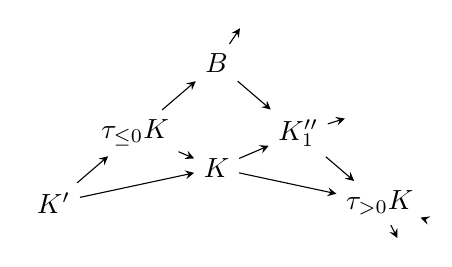
\begin{tikzpicture}[>=stealth,scale=.74]
\node(a)at(0,0){$K'$};\node(b)at(1.4,1.2){$\tau_{\leq0}K$};\node(c)at(2.8,2.4){$B$};\node(d)at(2.8,.6){$K$};\node(e)at(4.2,1.2){$K''_1$};\node(f)at(5.6,0){$\tau_{>0}K$};
\draw[->](a)--(b);\draw[->](b)--(c);\draw[->](c)--(e);\draw[->](e)--(f);\draw[->](a)--(d);\draw[->](b)--(d);\draw[->](d)--(e);\draw[->](d)--(f);\draw[->](c)--++(.4,.6);\draw[->](e)--++(.8,.25);\draw[->](f)--++(.7,-.25);\draw[->](f)--++(.3,-.6);
\end{tikzpicture}
\end{center}
三角 $(B,K''_1,\tau_{>0}K)$ 是 $K''_1$ 的1.3.1(iii)型三角，表明 $K''_1\in\mathcal D^{\geq0}$，且 $H^0K''_1=B$、$\tau_{>0}K\xrightarrow{\sim}\tau_{>0}K''_1$。由(ii)，$K''_1$ 与 $K''$ 等同，因此 $(K',K,K''_1)$ 就是(iii)中所需的三角。

\par\medskip\noindent\textbf{1.3.16.} 设 $\mathcal D_i$（$i=1,2$）是两个 $t$-范畴，$\mathcal C_i$ 是 $\mathcal D_i$ 的\term{heart}{心}，以 $\varepsilon$ 表示包含函子 $\mathcal C_i\hookrightarrow\mathcal D_i$。设 $T:\mathcal D_1\to\mathcal D_2$ 是\term{triangulated-category}{三角范畴}间的\term{exact-functor}{正合函子}（[10] 第4页）。若 $T(\mathcal D_1^{\leq0})\subset\mathcal D_2^{\leq0}$，则称 $T$ 右 \term{t-exact}{$t$-正合}；若 $T(\mathcal D_1^{\geq0})\subset\mathcal D_2^{\geq0}$，则称 $T$ 左 \term{t-exact}{$t$-正合}；同时左、右 \term{t-exact}{$t$-正合}时，称 $T$ 为 \term{t-exact}{$t$-正合}函子。

\par\medskip\noindent\textbf{命题1.3.17。} (i) 若 $T$ 左（相应地，右）\term{t-exact}{$t$-正合}，则加性函子 ${}^pT:=H^0\circ T\circ\varepsilon:\mathcal C_1\to\mathcal C_2$ 左（相应地，右）正合。
\SourcePage{44}
(ii) 若 $T$ 左（相应地，右）\term{t-exact}{$t$-正合}且 $K\in\mathcal D_1^{\geq0}$（相应地，$\mathcal D_1^{\leq0}$），则有 ${}^pTH^0K\xrightarrow{\sim}H^0TK$（相应地，$H^0TK\xrightarrow{\sim}{}^pTH^0K$）。

(iii) 设 $(T^*,T_*)$ 是一对互为\term{adjunction}{伴随}的\term{exact-functor}{正合函子}，其中 $T^*:\mathcal D_2\to\mathcal D_1$，$T_*:\mathcal D_1\to\mathcal D_2$ 是 $T^*$ 的右\term{adjunction}{伴随}。$T^*$ 右 \term{t-exact}{$t$-正合}的充要条件为 $T_*$ 左 \term{t-exact}{$t$-正合}；此时 $({}^pT^*,{}^pT_*)$ 构成一对\term{adjoint-functor}{伴随函子} $\mathcal C_1\rightleftarrows\mathcal C_2$。

(iv) 若 $T_1:\mathcal D_1\to\mathcal D_2$ 与 $T_2:\mathcal D_2\to\mathcal D_3$ 都左（相应地，右）\term{t-exact}{$t$-正合}，则 $T_2\circ T_1$ 也如此，且 ${}^p(T_2\circ T_1)={}^pT_2\circ{}^pT_1$。

若 $T$ 左 \term{t-exact}{$t$-正合}，则对 $\mathcal C_1$ 中每个短\term{exact-sequence}{正合列} $0\to X\to Y\to Z\to0$，\term{distinguished-triangle}{区别三角} $(T(X),T(Y),T(Z))$ 的\term{cohomology}{上同调}长\term{exact-sequence}{正合列}给出 $0\to H^0T(X)\to H^0T(Y)\to H^0T(Z)$，因为 $T(Z)\in\mathcal D_2^{\geq0}$。这就证明了(i)的左正合情形，右正合情形由\term{duality}{对偶}性得到。

对 $K\in\mathcal D_1^{\geq0}$，三角 $(H^0K,K,\tau_{>0}K)$ 给出三角 $(TH^0K,TK,T\tau_{>0}K)$，其中 $T\tau_{>0}K\in\mathcal D_2^{>0}$；其\term{cohomology}{上同调}长\term{exact-sequence}{正合列}给出 $H^0TH^0K\xrightarrow{\sim}H^0TK$。这与其\term{duality}{对偶}命题证明了(ii)。

若 $T_*$ 左 \term{t-exact}{$t$-正合}，对 $U\in\mathcal D_1^{>0}$、$V\in\mathcal D_2^{\leq0}$，有 $\Hom(T^*V,U)=\Hom(V,T_*U)=0$。这对每个 $U$ 都成立，因此 $\tau_{>0}T^*V=0$，即 $T^*V\in\mathcal D_1^{\leq0}$，所以 $T^*$ 右 \term{t-exact}{$t$-正合}。对 $A\in\mathcal C_1$、$B\in\mathcal C_2$，原文接着写为
\[
 H^0T^*B=\tau_{\leq0}T^*B,\qquad H^0T_*A=\tau_{\leq0}T_*A,
\]
从而有函子同构
\[
 \Hom(H^0T^*B,A)\xrightarrow{\sim}\Hom(T^*B,A)
 =\Hom(A,T_*B)\xleftarrow{\sim}\Hom(A,H^0T_*B).
\]
\footnote{译注：这里忠实保留原文的排印。由前述 \term{t-exact}{$t$-正合}性，第一式中的 $\tau_{\leq0}T^*B$ 应为 $\tau_{\geq0}T^*B$；\term{adjunction}{伴随}同构的右侧按对象所属范畴应为 $\Hom(B,T_*A)$ 及 $\Hom(B,H^0T_*A)$。}
这与\term{duality}{对偶}论证一起证明了(iii)。

若 $T_1,T_2$ 都左 \term{t-exact}{$t$-正合}且 $A\in\mathcal C_1$，则 $T_1A\in\mathcal D_2^{\geq0}$；由(ii)，有 ${}^p(T_2\circ T_1)A=H^0T_2T_1A=H^0T_2H^0T_1A$。这与\term{duality}{对偶}论证一起证明了(iv)。

\par\medskip\noindent\textbf{注1.3.18。} (i) 令 $\mathcal D_1^+=\bigcup_n\mathcal D_1^{\geq n}$、$\mathcal D_2^-=\bigcup_n\mathcal D_2^{\leq n}$。结论(iii)对 $T^*:\mathcal D_2^-\to\mathcal D_1$ 和 $T_*:\mathcal D_1^+\to\mathcal D_2$ 仍然成立；这里的“\term{adjunction}{伴随}”指对 $V\in\mathcal D_2^-$、$U\in\mathcal D_1^+$，函子性地有 $\Hom(T^*V,U)=\Hom(V,T_*U)$。证明相同。

(ii) 对 $A\in\mathcal C_1$、$B\in\mathcal C_2$，$(T^*,T_*)$ 与 $({}^pT^*,{}^pT_*)$ 的\term{adjunction}{伴随}箭头满足如下交换图：
\SourcePage{45}
\[
\begin{tikzcd}[ampersand replacement=\&,column sep=large]
 T^*{}^pT_*A\arrow[r]\arrow[d]\&{}^pT^*{}^pT_*A\arrow[d]\\
 T^*T_*A\arrow[r]\&A
\end{tikzcd}
\qquad\text{和}\qquad
\begin{tikzcd}[ampersand replacement=\&,column sep=large]
 B\arrow[r]\arrow[d]\&T_*T^*B\arrow[d]\\
 {}^pT_*{}^pT^*B\arrow[r]\&T_*{}^pT^*B.
\end{tikzcd}
\]

\par\medskip\noindent\textbf{1.3.19.} 设 $T:\mathcal D'\to\mathcal D$ 是\term{triangulated-category}{三角范畴}间的\term{fully-faithful}{全忠实}\term{exact-functor}{正合函子}。$\mathcal D'$ 的一个三角 $\mathrm{tr}$ 若在 $T$ 下的像 $T\mathrm{tr}$ 是\term{distinguished-triangle}{区别三角}，则它自身就是\term{distinguished-triangle}{区别三角}。事实上，取与 $\mathrm{tr}$ 底边相同的\term{distinguished-triangle}{区别三角} $\mathrm{tr}_1$；$T\mathrm{tr}$ 与 $T\mathrm{tr}_1$ 都是底边相同的\term{distinguished-triangle}{区别三角}，故二者同构，因而 $\mathrm{tr}$ 与 $\mathrm{tr}_1$ 同构。

假设 $\mathcal D,\mathcal D'$ 都配备 \term{t-structure}{$t$-结构}且 $T$ 为 \term{t-exact}{$t$-正合}函子。对 $X\in\mathcal D'$，若 $TX\in\mathcal D^{\leq0}$（相应地，$\mathcal D^{\geq0}$），则 $X\in\mathcal D'^{\leq0}$（相应地，$\mathcal D'^{\geq0}$）：这是因为 $X\in\mathcal D'^{\leq0}\Longleftrightarrow\tau_{>0}X=0$，而 $T$ 与 $\tau_{>0}$ 交换；另一情形\term{duality}{对偶}。

反之，若 $\mathcal D'$ 是\term{triangulated-category}{三角范畴} $\mathcal D$ 的全三角子范畴，且 $(\mathcal D^{\leq0},\mathcal D^{\geq0})$ 是 $\mathcal D$ 上的 \term{t-structure}{$t$-结构}，则
\[
 (\mathcal D'^{\leq0},\mathcal D'^{\geq0}):=(\mathcal D'\cap\mathcal D^{\leq0},\mathcal D'\cap\mathcal D^{\geq0})
\]
为 $\mathcal D'$ 上的 \term{t-structure}{$t$-结构}，当且仅当 $\mathcal D'$ 在函子 $\tau_{\leq0}$ 下稳定。满足此条件时，称所得结构为诱导 \term{t-structure}{$t$-结构}。对配备诱导 \term{t-structure}{$t$-结构}的 $\mathcal D'$，包含函子 $\mathcal D'\hookrightarrow\mathcal D$ 为 \term{t-exact}{$t$-正合}函子；有 $\mathcal C'=\mathcal D'\cap\mathcal C$，而 $\mathcal D$ 的函子 $\tau_{\leq p}$、$\tau_{\geq p}$、$H^p$ 限制到 $\mathcal D'$ 后，分别与 $\mathcal D'$ 的同名函子等同。

\par\medskip\noindent\textbf{1.3.20.} 设 $(\mathcal D_i)_{i\in I}$ 是有限族\term{triangulated-category}{三角范畴}，$T:\prod_i\mathcal D_i\to\mathcal D$ 是到\term{triangulated-category}{三角范畴} $\mathcal D$ 的正合多函子（SGA 4 XVII 1.1.3）。假设各 $\mathcal D_i$ 与 $\mathcal D$ 均配备 \term{t-structure}{$t$-结构}。若 $T$ 将各 $\mathcal D_i^{\geq0}$（相应地，$\mathcal D_i^{\leq0}$）的乘积映到 $\mathcal D^{\geq0}$（相应地，$\mathcal D^{\leq0}$），则称它左（相应地，右）\term{t-exact}{$t$-正合}；若左右均成立，则称它 \term{t-exact}{$t$-正合}。若 $T$ 左 \term{t-exact}{$t$-正合}（相应地，右 \term{t-exact}{$t$-正合}，或 \term{t-exact}{$t$-正合}），并将某些变量固定为 $\mathcal D_i^{\geq0}$（相应地，$\mathcal D_i^{\leq0}$，或 $\mathcal D_i$ 的\term{heart}{心} $\mathcal C_i$）中的给定对象，则所得关于其余变量的函子仍具有同样的 \term{t-exact}{$t$-正合}性。这使我们可以将单变量函子的结果应用于 $T$。例如：

令 $\varepsilon_i:\mathcal C_i\hookrightarrow\mathcal D_i$ 为包含函子，置 ${}^pT=H^0\circ T\circ(\varepsilon_i)_{i\in I}$。若 $T$ 左（相应地，右）\term{t-exact}{$t$-正合}，则从各 $\mathcal C_i$ 到 $\mathcal C$ 的加性多函子 ${}^pT$ 左（相应地，右）正合。

假设 $T$ 左 \term{t-exact}{$t$-正合}。对 $K_i\in\mathcal D_i^{\geq0}$，
\SourcePage{46}
由1.3.17(ii)有 ${}^pT(H^0K_i)\xrightarrow{\sim}H^0T(K_i)$。对任意 $K_i$，态射 $K_i\to\tau_{\geq0}K_i$ 给出态射
\begin{equation*}
 H^0T(K_i)\longrightarrow H^0T(\tau_{\geq0}K_i)\xleftarrow{\sim}{}^pT(H^0K_i).\tag{1.3.20.1}
\end{equation*}
作平移后，更一般地，当 $\sum_i n_i=n$ 时，得到态射
\begin{equation*}
 H^nT(K_i)\longrightarrow{}^pT(H^{n_i}K_i).\tag{1.3.20.2}
\end{equation*}
这里有符号问题；若改为考虑
\begin{equation*}
 H^nT(K_i)\longrightarrow H^nT\bigl((H^{n_i}K_i)[-n_i]\bigr),\tag{1.3.20.3}
\end{equation*}
就不会出现这一问题。

若 $T$ 右 \term{t-exact}{$t$-正合}，则对 $K_i\in\mathcal D_i^{\leq0}$ 有 ${}^pTH^0K_i\xleftarrow{\sim}H^0TK_i$；态射 $\tau_{\leq0}K_i\to K_i$ 给出态射 ${}^pT(H^0K_i)\to H^0T(K_i)$，再作平移得到
\begin{equation*}
 H^nT\bigl((H^{n_i}K_i)[-n_i]\bigr)\longrightarrow H^nT(K_i)
 \qquad\left(\sum_i n_i=n\right).\tag{1.3.20.4}
\end{equation*}
若 $T$ 为 \term{t-exact}{$t$-正合}函子，则(1.3.20.3)、(1.3.20.4)同时存在。将 $H^nT$ 应用于交换图
\[
\begin{tikzcd}[ampersand replacement=\&,column sep=large]
 \tau_{\leq n_i}K_i\arrow[r]\arrow[d]\&H^{n_i}K_i[-n_i]\arrow[d]\\
 K_i\arrow[r]\&\tau_{\geq n_i}K_i
\end{tikzcd}
\]
可知复合 $(1.3.20.3)\circ(1.3.20.4)$ 是恒等态射。若 $\sum_i n_i=\sum_i m_i=n$ 且 $(n_i)_{i\in I}\neq(m_i)_{i\in I}$，则存在某个 $i$ 使 $n_i<m_i$。复合 $\tau_{\leq n_i}K_i\to K_i\to\tau_{\geq m_i}K_i$ 为零，因此“$(m_i)$ 对应的(1.3.20.3)”与“$(n_i)$ 对应的(1.3.20.4)”的复合也为零。

\par\medskip\noindent\textbf{命题1.3.21。} 若 $T$ 为 \term{t-exact}{$t$-正合}函子且 $K_i\in\mathcal D_i^b$，则态射(1.3.20.3)和(1.3.20.4)定义互为逆的同构
\begin{equation*}
 H^nT(K_i)\simeq\bigoplus_{\sum_i n_i=n}H^nT\bigl((H^{n_i}K_i)[-n_i]\bigr).\tag{1.3.21.1}
\end{equation*}
我们已经看到，这些态射使右侧成为左侧的一个直和因子。(1.3.21.1)两侧关于每个 $K_i$ 都是\term{cohomological-functor}{上同调函子}（对右侧，这是因为 ${}^pT$ 正合）；(1.3.20.3)与(1.3.20.4)是\term{cohomological-functor}{上同调函子}之间的态射。通过逐次分解，归结为各 $K_i\in\mathcal C_i$ 的情形；此时结论显然。

\SourcePage{47}
\par\medskip\noindent\textbf{1.3.22. \term{t-structure}{$t$-结构}的例子。} （本文后续部分不会使用。）

如1.1.4，设 $A$ 为\term{exact-category}{正合范畴}，$E$ 为其短\term{exact-sequence}{正合列}的集合。假设每个态射 $f:A\to B$ 都有核，且 $\Ker(f)\to A$ 可嵌入短\term{exact-sequence}{正合列} $0\to\Ker(f)\to A\to\mathrm{Coim}(f)\to0$。令 $\mathcal D^{\leq0}$（相应地，$\mathcal D^{\geq0}$）为 $\mathcal D:=DA$（1.1.4）的子范畴，由满足当 $i>0$（相应地，$i<0$）时态射 $\mathrm{Coim}(d^{i-1})\to\Ker(d^i)$ 为同构的\term{complex}{复形} $K$ 组成。用嵌入 $h:A\to(A,E)^{\sim}$（1.1.4）来表述，就是 $K$ 在 $D((A,E)^{\sim})$ 中的像 $h_K$ 属于 $D^{\leq0}$（相应地，$D^{\geq0}$）。来证明 $(\mathcal D^{\leq0},\mathcal D^{\geq0})$ 是 $\mathcal D$ 上的 \term{t-structure}{$t$-结构}。

(a) 对 $K,L\in\mathcal D$，有 $\Hom_{\mathcal D}(K,L)=\varinjlim\Hom_{KA}(K',L')$，极限取遍\term{quasi-isomorphism}{拟同构} $K'\to K$ 与 $L\to L'$ 的\term{homotopy}{同伦}类。若 $K\in\mathcal D^{\leq0}$（相应地，$L\in\mathcal D^{\geq1}$），则可以将 $K'$（相应地，$L'$）限制为满足 $i>0$ 时 $K'^i=0$（相应地，$i<0$ 时 $L'^i=0$）的对象，而仍得到\term{cofinal}{余尾}系统；只须使用\term{quasi-isomorphism}{拟同构} $\tau_{\leq0}K'\to K'$（相应地，$L'\to\tau_{\geq1}L'$），其中 $\tau_{\leq0}$、$\tau_{\geq1}$ 如1.3.2(i)所定义。对这样的 $K',L'$，每个\term{complex}{复形}态射 $f:K'\to L'$ 都为零：它由满足 $df^0=0$ 的 $f^0:K'^0\to L'^0$ 决定，而 $d:L'^0\to L'^1$ 是单态射，故 $f^0=0$。这验证了1.3.1(i)。公理1.3.1(ii)显然。

(b) 对 $K\in KA$，有\term{complex}{复形}短\term{exact-sequence}{正合列} $0\to\tau_{\leq0}K\to K\to\tau_{\geq1}K\to0$。它定义 $DA$ 中的\term{distinguished-triangle}{区别三角}：$\tau_{\leq0}K\to K$ 的\term{cone}{锥}\term{quasi-isomorphism}{拟同构}地映到 $\tau_{\geq1}K$。这验证了1.3.1(iii)。

特别地，$\mathcal D$ 的\term{heart}{心} $\mathcal C$ 是\term{abelian-category}{阿贝尔范畴}。$\mathcal C$ 的对象可表示为长为1的\term{complex}{复形} $K^{-1}\xrightarrow{d}K^0$，其中 $d$ 是单态射。对这样的 $K,L$，一个\term{complex}{复形}态射 $f:K\to L$ 由其分量 $f^0:K^0\to L^0$ 唯一确定。若将 $K^{-1}$、$L^{-1}$ 分别与 $K^0$、$L^0$ 的子对象等同，则 $f^0:K^0\to L^0$ 来自\term{complex}{复形}态射 $f$ 当且仅当 $f^0(K^{-1})\subset L^{-1}$；而 $f$ \term{homotopy}{同伦}于零，当且仅当 $f^0(K^0)\subset L^{-1}$。$f$ 是\term{quasi-isomorphism}{拟同构}，意味着列
\[
 0\longrightarrow K^{-1}\longrightarrow K^0\oplus L^{-1}\longrightarrow L^0\longrightarrow0
\]
正合，即 $K^0\oplus L^{-1}\to L^0$ 是\term{admissible}{容许}满态射，且 $K^0$ 的子对象 $K^{-1}$ 是 $L^{-1}$ 沿 $f^0$ 的拉回。

容易验证，若 $K'\xrightarrow{\varphi}K$ 是一个\term{quasi-isomorphism}{拟同构}，
\SourcePage{48}
其中 $K'$ 集中于0次与 $-1$ 次，且 $f\varphi$ \term{homotopy}{同伦}于零（即 $f\varphi(K'^0)\subset L^{-1}$），则 $f$ 也\term{homotopy}{同伦}于零。群 $\Hom_{\mathcal C}(K,L)$ 是如下群关于这种\term{quasi-isomorphism}{拟同构} $\varphi:K'\to K$ 的归纳极限：
\[
 \Hom_{KA}(K',L)=
 \frac{\{f:K'^0\to L^0\mid f(K'^{-1})\subset L^{-1}\}}
 {\{f\mid f(K'^0)\subset L^{-1}\}};
\]
而此归纳极限中的过渡态射都是单射。

\par\medskip\noindent\textbf{1.3.23. 习题。} (i) 对 $A$ 中对象的\term{complex}{复形} $K$，$\mathcal C$ 中的 $H^0K$ 是\term{complex}{复形} $\mathrm{Coim}(d^{-1})\to\Ker(d^0)$。

(ii) 若函子 $F$ 从 $A$ 到\term{abelian-category}{阿贝尔范畴} $N$，并将 $E$ 中的列变为右\term{exact-sequence}{正合列} $FA\to FB\to FC\to0$，则它可唯一地（在唯一同构意义下）延拓为右\term{exact-functor}{正合函子} $F':\mathcal C\to N$。若 $F$ \term{fully-faithful}{全忠实}，并将 $E$ 中的列变为短\term{exact-sequence}{正合列}，将单态射变为单态射，则 $F'$ 正合且\term{fully-faithful}{全忠实}。特别地，复合函子
\[
 \mathcal C\longrightarrow DA\longrightarrow D((A,E)^{\sim})\xrightarrow{H^0}(A,E)^{\sim}
\]
是\term{fully-faithful}{全忠实}的；它将 $\mathcal C$ 与 $(A,E)^{\sim}$ 中由一个 $A$ 的对象除以一个仍属于 $A$ 的子对象所得的商组成的范畴等同。

(iii) 函子 $D^-A\to D^-\mathcal C$ 是\term{equivalence}{等价}（上标 $-$ 表示只考虑有上界的\term{complex}{复形}）。［利用每个 $\mathcal C$ 的对象都是某个 $A$ 的对象的商。］

(iv) 设 $A$ 是\term{abelian-category}{阿贝尔范畴}。$FA$ 满足1.3.22的假设（1.1.3例2）。设 $\mathcal C$ 是相应的\term{filtration}{滤过}对象的\term{formal-quotient}{形式商}所成的\term{abelian-category}{阿贝尔范畴}；设 $\mathcal C'$ 为列 $\cdots\to A^i\to A^{i-1}\to\cdots$ 所成的范畴，其中 $i\gg0$ 时 $A^i=0$，$i\ll0$ 时 $A^i\xrightarrow{\sim}A^{i-1}$。证明从 $\mathcal C$ 到 $\mathcal C'$ 的函子
\[
 ((V^{-1},F)\longrightarrow(V^0,F))\longmapsto
 \bigl(\Coker(F^iV^{-1}\to F^iV^0)\bigr)_i
\]
是\term{equivalence}{等价}。［应用(ii)。］

\par\medskip\noindent\textbf{1.3.24. 例。} 取 $A$ 为 Banach 空间范畴，将忘掉拓扑后变为短\term{exact-sequence}{正合列}的列作为短\term{exact-sequence}{正合列}，则1.3.22的假设成立。由\term{closed-graph-theorem}{闭图像定理}，这些列就是同构于 $0\to A\to B\to C\to0$ 的列，其中 $A$ 是 $B$ 的闭子空间，$C=B/A$。所得范畴 $\mathcal C$ 是“\term{formal-quotient}{形式商}” $B/A$ 所成的范畴（这里 $A\to B$ 是 Banach 空间之间的连续单射线性映射）。\term{closed-graph-theorem}{闭图像定理}保证：若\term{complex}{复形} $K^{-1}\to K^0$ 与 $L^{-1}\to L^0$ 定义 $\mathcal C$ 的对象，则一个\term{complex}{复形}态射 $f:K\to L$ 等同于连续线性映射 $f^0:K^0\to L^0$，且在集合意义下 $f(K^{-1})\subset L^{-1}$；而 $f$ \term{homotopy}{同伦}于零（即在 $\mathcal C$ 中为零），当且仅当在集合意义下 $f(K^0)\subset L^{-1}$。
\SourcePage{49}
L. Walbroeck 曾考虑过类似的\term{formal-quotient}{形式商}（\emph{Les quotients de b-espaces}，预印本，Bruxelles，1962）。

% PDF物理页50--62；原印刷页43--55。第1.4节完整译文。
\SourcePage{50}
\section*{1.4. 粘合}
\addcontentsline{toc}{section}{1.4. 粘合}

\par\medskip\noindent\textbf{1.4.1.}
设 $X$ 是带有环\term{sheaf}{层} $\mathcal O$ 的拓扑空间（也可以是一个\term{topos}{拓扑斯}）。记 $\D(X,\mathcal O)$ 为 $X$ 上左 $\mathcal O$-模\term{sheaf}{层}所成的\term{abelian-category}{阿贝尔范畴} $M(X,\mathcal O)$ 的\term{derived-category}{导出范畴}。照常，以 $\D^+(X,\mathcal O)$ 表示由下有界\term{complex}{复形}的\term{essential-image}{本质像}构成的满子范畴。

设 $U$ 是 $X$ 的一个开子集，$F$ 是其闭补集，$j$ 和 $i$ 分别为 $U$ 和 $F$ 到 $X$ 的包含映射；$\mathcal O$ 在 $U$ 或 $F$ 上的\term{inverse-image}{逆像}仍记作 $\mathcal O$。下面要给出一种构造：由 $\D^+(U,\mathcal O)$ 和 $\D^+(F,\mathcal O)$ 上各自的一个\term{t-structure}{$t$-结构}，得到 $\D^+(X,\mathcal O)$ 上的一个 \term{t-structure}{$t$-结构}。

范畴 $M(X,\mathcal O)$、$M(U,\mathcal O)$ 和 $M(F,\mathcal O)$ 之间有以下函子：
\[
\begin{aligned}
j_! &:M(U,\mathcal O)\longrightarrow M(X,\mathcal O),&&\text{\term{extension-by-zero}{零延拓}（正合）；}\\
j^* &:M(X,\mathcal O)\longrightarrow M(U,\mathcal O),&&\text{限制（正合），也记作 }j^!;\\
j_* &:M(U,\mathcal O)\longrightarrow M(X,\mathcal O),&&\text{\term{direct-image}{正像}（左正合）；}\\
i^* &:M(X,\mathcal O)\longrightarrow M(F,\mathcal O),&&\text{限制（正合）；}\\
i_* &:M(F,\mathcal O)\longrightarrow M(X,\mathcal O),&&\text{\term{direct-image}{正像}（正合），也记作 }i_!;\\
i^! &:M(X,\mathcal O)\longrightarrow M(F,\mathcal O),&&\text{\term{support}{支撑}于 }F\text{ 的截面（左正合）。}
\end{aligned}
\]
它们组成两个由三个\term{adjunction}{伴随}函子构成的序列 $(j_!,j^!=j^*,j_*)$ 和 $(i^*,i_*=i_!,i^!)$。有 $j^*i_*=0$，由\term{adjunction}{伴随}性又得 $i^*j_!=0$ 和 $i^!j_*=0$。对 $X$ 上的每个\term{sheaf}{层} $\mathcal F$，\term{adjunction-morphism}{伴随态射}给出\term{exact-sequence}{正合列}
\begin{equation*}
\begin{gathered}
0\longrightarrow j_!j^*\mathcal F\longrightarrow\mathcal F
 \longrightarrow i_*i^*\mathcal F\longrightarrow0,\\
0\longrightarrow i_*i^!\mathcal F\longrightarrow\mathcal F
 \longrightarrow j_*j^*\mathcal F.
\end{gathered}\tag{1.4.1.1}
\end{equation*}
当 $\mathcal F$ \term{injective}{内射}时，第二列的右端可以补上一个 $0$。

对 $F$ 上（分别地，$U$ 上）的 $\mathcal F$，\term{adjunction-morphism}{伴随态射}给出同构
\begin{equation*}
i^*i_*\mathcal F\xrightarrow{\sim}\mathcal F
 \xrightarrow{\sim}i^!i_*\mathcal F,\tag{1.4.1.2}
\end{equation*}
\begin{equation*}
j^*j_*\mathcal F\xrightarrow{\sim}\mathcal F
 \xrightarrow{\sim}j^*j_!\mathcal F.\tag{1.4.1.3}
\end{equation*}
对任意一对\term{adjoint-functor}{伴随函子} $(T^*,T_*)$，\term{adjunction-morphism}{伴随态射} $T^*T_*\to\mathrm{Id}$（分别地，$\mathrm{Id}\to T_*T^*$）为同构，当且仅当 $T_*$（分别地，$T^*$）\term{fully-faithful}{全忠实}。因此，断言 (1.4.1.2)、(1.4.1.3) \term{equivalence}{等价}于说：$i_*$、$j_*$ 和 $j_!$ \term{fully-faithful}{全忠实}。

\par\medskip\noindent\textbf{1.4.2.0.}
\term{abelian-category}{阿贝尔范畴}之间的\term{exact-functor}{正合函子} $T$ 可以直接诱导出\term{derived-category}{导出范畴}之间的函子。我们往往
\SourcePage{51}
用同一符号表示原函子及其在\term{derived-category}{导出范畴}上的延拓。这个延拓既是 $T$ 的左导出函子 $LT$，也是其右导出函子 $RT$。

\par\medskip\noindent\textbf{1.4.2.1.}
1.4.1 中的函子经右导出后，给出连接 $\D^+(X,\mathcal O)$、$\D^+(U,\mathcal O)$ 和 $\D^+(F,\mathcal O)$ 的函子，组成两个\term{adjoint-functor}{伴随函子}三元组 $(j_!,j^*,Rj_*)$ 和 $(i^*,i_*,Ri^!)$。有 $j^*i_*=0$；由\term{adjunction}{伴随}性，$i^*j_!=0$ 且 $Ri^!Rj_*=0$。对 $K^+(X,\mathcal O)$ 中的任意 $K$，\term{exact-sequence}{正合列} (1.4.1.1) 导出为\term{distinguished-triangle}{区别三角}
\[
(j_!j^*K,K,i_*i^*K),\qquad(i_*Ri^!K,K,Rj_*j^*K).
\]
对 $\D^+(F,\mathcal O)$ 中（分别地，$\D^+(U,\mathcal O)$ 中）的 $K$，(1.4.1.2)（分别地，(1.4.1.3)）给出同构
\[
i^*i_*K\xrightarrow{\sim}K\xrightarrow{\sim}Ri^!i_*K:
 \quad i_*\text{ \term{fully-faithful}{全忠实}},
\]
\[
\text{（分别为 }j^*Rj_*K\xrightarrow{\sim}K\xrightarrow{\sim}j^*j_!K:
 \quad j_!\text{ 和 }Rj_*\text{ \term{fully-faithful}{全忠实}）。}
\]
这是因为 $j_*$ 和 $i_*$ 将\term{injective}{内射}对象送到\term{injective}{内射}对象。

\par\medskip\noindent\textbf{1.4.2.3.}
\term{recollement}{粘合} \term{t-structure}{$t$-结构}时，我们只需要上面列出的这些性质。在其他情形中也会遇到它们，例如严格说来不属于 1.4.1 框架的 \term{l-adic}{$\ell$-进}\term{derived-category}{导出范畴}。为了涵盖这些情形，下面采用 1.4.3 中更一般的框架。在这一框架内，不再出现\term{sheaf}{层}范畴，只出现\term{triangulated-category}{三角范畴}；我们也借此简化记号，把上面的 $Rj_*$ 和 $Ri^!$ 分别直接写作 $j_*$ 和 $i^!$。

\par\medskip\noindent\textbf{1.4.3.}
设有三个\term{triangulated-category}{三角范畴} $\mathcal D$、$\mathcal D_U$ 和 $\mathcal D_F$，以及\term{exact-functor}{正合函子}
\[
\mathcal D_F\xrightarrow{i_*}\mathcal D\xrightarrow{j^*}\mathcal D_U.
\]
有时令 $i_!:=i_*$、$j^!:=j^*$，会更方便。我们假定下面的 (1.4.3.1)--(1.4.3.5) 成立。

\par\medskip\noindent\textbf{(1.4.3.1)} $i_*$ 有正合的左、右\term{adjoint-functor}{伴随函子}，分别记为 $i^*$ 和 $i^!$。

\par\medskip\noindent\textbf{(1.4.3.2)} $j^*$ 有正合的左、右\term{adjoint-functor}{伴随函子}，分别记为 $j_!$ 和 $j_*$。

\par\medskip\noindent\textbf{(1.4.3.3)} 有 $j^*i_*=0$。因此，由\term{adjunction}{伴随}性还有 $i^*j_!=0$ 和 $i^!j_*=0$，并且对 $\mathcal D_F$ 中的 $A$ 和 $\mathcal D_U$ 中的 $B$，有
\[
\Hom(j_!B,i_*A)=0,\qquad\Hom(i_*A,j_*B)=0.
\]
\SourcePage{52}
\par\medskip\noindent\textbf{(1.4.3.4)} 对 $\mathcal D$ 中的任意 $K$，存在
\[
d:i_*i^*K\longrightarrow j_!j^*K[1]
\quad\text{（分别地， }d:j_*j^*K\longrightarrow i_*i^!K[1]\text{），}
\]
使三角
\[
j_!j^*K\longrightarrow K\longrightarrow i_*i^*K\xrightarrow{d},
\]
\[
\text{（分别为 }i_*i^!K\longrightarrow K\longrightarrow j_*j^*K\xrightarrow{d}\text{）}
\]
为\term{distinguished-triangle}{区别三角}。由 (1.4.3.3) 和 1.1.10，$d$ 唯一。

\par\medskip\noindent\textbf{(1.4.3.5)} $i_*$、$j_!$ 和 $j_*$ \term{fully-faithful}{全忠实}，即\term{adjunction-morphism}{伴随态射}
\[
i^*i_*\longrightarrow\mathrm{Id}\longrightarrow i^!i_*,
\qquad j^*j_*\longrightarrow\mathrm{Id}\longrightarrow j^*j_!
\]
均为同构。

这一套形式体系是\term{self-dual}{自对偶}的；\term{duality}{对偶}交换 $j_!$ 与 $j_*$，也交换 $i^*$ 与 $i^!$。

\par\medskip\noindent\textbf{1.4.4.}
设\term{triangulated-category}{三角范畴} $\mathcal T$ 带有两个严格满子范畴 $\mathcal U$ 和 $\mathcal V$，它们在平移 $X\mapsto X[n]$（$n\in\Z$）下稳定。假定对 $\mathcal U$ 中的 $U$ 和 $\mathcal V$ 中的 $V$，有 $\Hom(U,V)=0$，并且每个 $\mathcal T$ 中的 $X$ 都能置于一个\term{distinguished-triangle}{区别三角} $(U,X,V)$ 中，其中 $U\in\mathcal U$、$V\in\mathcal V$。于是 $(\mathcal U,\mathcal V)$ 是 $\mathcal T$ 上的一个 \term{t-structure}{$t$-结构}。由 1.3.4，$\mathcal V$ 是 $\mathcal U$ 的右正交，$\mathcal U$ 是 $\mathcal V$ 的左正交。特别地，$\mathcal U$ 和 $\mathcal V$ 是\term{thick-subcategory}{厚子范畴}（[10] 6.2，第24页）。[10] 6.4（第25页）的假设 (i)、(ii) 成立；由 [10] 第23--26页，投影 $\mathcal T\to\mathcal T/\mathcal U$ 有一个\term{fully-faithful}{全忠实}的右\term{adjoint-functor}{伴随函子}，其像为 $\mathcal V$；投影 $\mathcal T\to\mathcal T/\mathcal V$ 则有一个\term{fully-faithful}{全忠实}的左\term{adjoint-functor}{伴随函子}，其像为 $\mathcal U$。换言之，包含函子 $u:\mathcal U\to\mathcal T$（分别地，$v:\mathcal V\to\mathcal T$）有右\term{adjunction}{伴随}（分别地，左\term{adjunction}{伴随}）$u_*$（分别地，$v^*$），而序列
\[
0\longrightarrow\mathcal U\xrightarrow{u}\mathcal T\xrightarrow{v^*}\mathcal V\longrightarrow0,
\qquad
0\longleftarrow\mathcal U\xleftarrow{u_*}\mathcal T\xleftarrow{v}\mathcal V\longleftarrow0
\]
在如下意义下“正合”：$v^*$（分别地，$u_*$）把 $\mathcal V$（分别地，$\mathcal U$）等同于 $\mathcal T$ 对\term{thick-subcategory}{厚子范畴} $\mathcal U$（分别地，$\mathcal V$）的商。

取 $\mathcal T=\mathcal D$，并分别取 $(\mathcal U,\mathcal V)$ 为 $(i_*\mathcal D_F,j_*\mathcal D_U)$ 和 $(j_!\mathcal D_U,i_*\mathcal D_F)$，就得到：

\par\medskip\noindent\textbf{命题 1.4.5.} 下列序列在上述意义下“正合”：
\[
\begin{gathered}
0\longleftarrow\mathcal D_F\xleftarrow{i^*}\mathcal D\xleftarrow{j_!}\mathcal D_U\longleftarrow0,\\
0\longrightarrow\mathcal D_F\xrightarrow{i_*}\mathcal D\xrightarrow{j^*}\mathcal D_U\longrightarrow0,\\
0\longleftarrow\mathcal D_F\xleftarrow{i^!}\mathcal D\xleftarrow{j_*}\mathcal D_U\longleftarrow0.
\end{gathered}
\]

\par\medskip\noindent\textbf{1.4.6.}
a) 函子 $i_*$ \term{fully-faithful}{全忠实}，所以\term{adjunction-morphism}{伴随态射}的复合 $i_*i^!\to\mathrm{Id}\to i_*i^*$ 是某个唯一的函子态射经 $i_*$ 作用所得。这个函子态射为
\SourcePage{53}
\begin{equation*}
i^!\longrightarrow i^*.\tag{1.4.6.1}
\end{equation*}
将其作用于 $i_*X$，并把 $i^!i_*X$ 和 $i^*i_*X$ 均等同于 $X$ 后，得到的是 $X$ 的恒等自同构。

b) 函子 $j^*$ 是取商函子（它把 $\mathcal D_U$ 等同于由 $\mathcal D$ 经分式演算得到的范畴），所以\term{adjunction-morphism}{伴随态射}的复合 $j_!j^*\to\mathrm{Id}\to j_*j^*$ 来自某个唯一的函子态射
\begin{equation*}
j_!\longrightarrow j_*.\tag{1.4.6.2}
\end{equation*}
若把 $j^*j_!$ 和 $j^*j_*$ 均等同于恒等函子，则对 (1.4.6.2) 作用 $j^*$ 后，得到恒等函子的恒等自同构。

c) 对 $\mathcal D_U$ 中的 $X$，$j_!X\to j_*X$ 的\term{cone}{锥}因而被 $j^*$ \term{effaceable}{消去}，故属于 $i_*\mathcal D_F$。由 (1.4.3.3) 和 1.1.10，以 $j_!X\to j_*X$ 为底的\term{distinguished-triangle}{区别三角}在唯一同构意义下唯一。因此得到函子 $j_*/j_!:\mathcal D_U\to\mathcal D_F$，以及函子性的\term{distinguished-triangle}{区别三角}
\begin{equation*}
(j_!,j_*,i_*(j_*/j_!)).\tag{1.4.6.3}
\end{equation*}
\term{duality}{对偶}的构造给出函子 $T:\mathcal D_U\to\mathcal D_F$，它由函子性的\term{distinguished-triangle}{区别三角} $(i_*T,j_!,j_*)$ 刻画。这类三角可由 (1.4.6.3) 旋转得到，因此有同构
\[
T=(j_*/j_!)[-1],
\]
使得态射 $i_*T\to j_!$ 是 (1.4.6.3) 中次数为 $1$ 的态射经 $[-1]$ 平移所得。于是，函子 $(j_*/j_!)$ 和 $(j_*/j_!)[-1]$ 互为\term{duality}{对偶}。

对 (1.4.6.3) 作用函子 $i^*$ 和 $i^!$，并利用 $i^*j_!=i^!j_*=0$，得到同构
\begin{equation*}
i^*j_*\xrightarrow{\sim}j_*/j_!\xrightarrow{\sim}i^!j_![1].\tag{1.4.6.4}
\end{equation*}

\par\medskip\noindent\textbf{1.4.7.}
设 $X\in\mathcal D$，对\term{adjunction-morphism}{伴随态射} $j_!j^*X\to X\to j_*j^*X$ 应用 TR~4。下面证明所得八面体在唯一同构意义下唯一，并且关于 $X$ 具有函子性。
\[
\begin{tikzcd}[ampersand replacement=\&,column sep=large,row sep=large]
\&\&A\arrow[dr]\arrow[ddll,bend right=40,"{+1}"']\&\&\\
\&X\arrow[ur]\arrow[dr]\&\&B\arrow[dr]\arrow[dlll,bend left=30,"{+1}"]\&\\
j_!j^*X\arrow[ur]\arrow[rr]\&\&j_*j^*X\arrow[ur]\arrow[rr]\&\&C\arrow[ulll,bend left=28,"{+1}"]\arrow[uull,bend right=38,"{+1}"']
\end{tikzcd}
\]
% 上图以平面展开方式重绘八面体；各标有+1的箭头均为次数1的连接态射。
(a) 由 (1.4.3.3)、(1.4.3.4) 和 1.1.10，存在唯一同构 $A=i_*i^*X$，它把 $X\to A$ 等同于\term{adjunction}{伴随}箭头。
\SourcePage{54}
这个同构将 $(j_!j^*X,X,A)$ 等同于 (1.4.3.4) 中的\term{distinguished-triangle}{区别三角} $(j_!j^*X,X,i_*i^*X)$。

(b) 把同一论证用于与 $X$ 有相同 $j^*$ 的对象 $j_*j^*X$，就把 $B$ 等同于
\[
i_*i^*j_*j^*X=i_*(j_*/j_!)j^*X\qquad\text{(1.4.6.4)，}
\]
其中 $j_*j^*X\to B$ 是 $(i^*,i_*)$ 的\term{adjunction}{伴随}箭头。由 1.1.9，存在唯一态射 $A\to B$，使八面体上方的菱形交换。因此，态射 $A\to B$，即 $i_*i^*X\to i_*i^*j_*j^*X$，正是由 $X\to j_*j^*X$ 根据函子性得到的态射。

(c) \term{duality}{对偶}地，存在唯一同构 $C=i_*i^!X[1]$，它将 $(X,j_*j^*X,C)$ 中次数为 $1$ 的箭头等同于\term{adjunction-morphism}{伴随态射} $i_*i^!X\to X$：三角 $(X,j_*j^*X,C)$ 由 (1.4.3.4) 中的三角 $(i_*i^!X,X,j_*j^*X)$ 旋转（TR~2）而来，同时改变 $j_*j^*X\xrightarrow{(1)}i_*i^!X$ 的符号。态射 $B\to C$ 是使正方形 $(B,C,j_!j^*X,X)$ 交换的唯一态射。通过 (1.4.6.4) 中 $j_*/j_!$ 与 $i^!j_![1]$ 的同构，它就是由 $j_!j^*X\to X$ 根据函子性得到的态射
\[
i_*(j_*/j_!)j^*X=i_*i^!j_!j^*X[1]\longrightarrow i_*i^!X[1].
\]
(d) 至此，八面体的全部顶点和箭头都已确定（$C\xrightarrow{(1)}A$ 是 $C\xrightarrow{(1)}X\to A$ 的复合），并且函子性也得到了证明。代入 $A$、$B$、$C$ 的值，八面体为
\begin{equation*}
\begin{tikzcd}[ampersand replacement=\&,column sep=small,row sep=large]
\&\&i_*i^*X\arrow[dr]\arrow[ddll,bend right=40,"{+1}"']\&\&\\
\&X\arrow[ur]\arrow[dr]\&\&i_*(j_*/j_!)j^*X\arrow[dr]\arrow[dlll,bend left=30,"{+1}"]\&\\
j_!j^*X\arrow[ur]\arrow[rr]\&\&j_*j^*X\arrow[ur]\arrow[rr]\&\&i_*i^!X[1]\arrow[ulll,bend left=28,"{+1}"]\arrow[uull,bend right=38,"{+1}"']
\end{tikzcd}\tag{1.4.7.1}
\end{equation*}
因为 $i_*$ \term{fully-faithful}{全忠实}，\term{distinguished-triangle}{区别三角}
\[
(i_*i^*X,i_*(j_*/j_!)j^*X,i_*i^!X[1])
\]
是三角 $(i^*X,(j_*/j_!)j^*X,i^!X[1])$ 经 $i_*$ 作用所得；后者自动是\term{distinguished-triangle}{区别三角}（1.3.19）。这个三角中次数为 $1$ 的箭头 $d$ 经 $i_*$ 作用后，是复合
\[
i_*i^!X[1]\xrightarrow{(1)}X\longrightarrow i_*i^*X.
\]
因此，$d$ 就是 $X[1]$ 对应的 (1.4.6.1)，也即 $X$ 对应的 (1.4.6.1) 经 $[1]$ 作用所得。旋转三角（TR~2），改变新的次数 $1$ 箭头的符号，再去掉 $i_*$（1.3.19），便得到以 (1.4.6.1) 为底的函子性\term{distinguished-triangle}{区别三角}
\begin{equation*}
(i^!,i^*,(j_*/j_!)j^*).\tag{1.4.7.2}
\end{equation*}
在 1.4.1、1.4.2 的框架内，这个三角来自如下事实：对每个\term{flabby-sheaf}{松弛层} $\mathcal F$，序列
\[
0\longrightarrow i^!\mathcal F\longrightarrow i^*\mathcal F
 \longrightarrow i^*j_*j^*\mathcal F\longrightarrow0
\]
正合。

\SourcePage{55}
\par\medskip\noindent\textbf{注 1.4.8.}
根据 [10] 第2节，特别是第23--27页，公理 (1.4.3.1)--(1.4.3.5) \term{equivalence}{等价}于：“$i_*$ 把 $\mathcal D_F$ 等同于 $\mathcal D$ 的一个\term{thick-subcategory}{厚子范畴}；$j^*$ 把 $\mathcal D_U$ 等同于 $\mathcal D/\mathcal D_F$，且 $j^*$ 有左\term{adjunction}{伴随}和右\term{adjunction}{伴随}。”

\par\medskip\noindent\textbf{1.4.9.}
假定 1.4.3 的条件成立，且 $(\mathcal D_U^{\le0},\mathcal D_U^{\ge0})$ 是 $\mathcal D_U$ 上的 \term{t-structure}{$t$-结构}，$(\mathcal D_F^{\le0},\mathcal D_F^{\ge0})$ 是 $\mathcal D_F$ 上的 \term{t-structure}{$t$-结构}。定义
\[
\begin{aligned}
\mathcal D^{\le0}&:=\{K\in\mathcal D\mid j^*K\in\mathcal D_U^{\le0},\ i^*K\in\mathcal D_F^{\le0}\},\\
\mathcal D^{\ge0}&:=\{K\in\mathcal D\mid j^*K\in\mathcal D_U^{\ge0},\ i^!K\in\mathcal D_F^{\ge0}\}.
\end{aligned}
\]

\par\medskip\noindent\textbf{定理 1.4.10.}
在上述假设与记号下，$(\mathcal D^{\le0},\mathcal D^{\ge0})$ 是 $\mathcal D$ 上的一个 \term{t-structure}{$t$-结构}。我们称它是由 $\mathcal D_U$ 和 $\mathcal D_F$ 上的 \term{t-structure}{$t$-结构}经\term{recollement}{粘合}得到的。

下面验证公理 1.3.1 (i)、(ii)、(iii)。

\emph{公理 (i)。} 设 $X\in\mathcal D^{\le0}$、$Y\in\mathcal D^{\ge1}$。对 $X$ 应用 (1.4.3.4) 中的第一个三角，得到\term{exact-sequence}{正合列}
\[
\Hom(i_*i^*X,Y)\longrightarrow\Hom(X,Y)\longrightarrow\Hom(j_!j^*X,Y).
\]
由 $\mathcal D_F$ 上的 1.3.1 (i)，有 $\Hom(i_*i^*X,Y)=\Hom(i^*X,i^!Y)=0$；由 $\mathcal D_U$ 上的 1.3.1 (i)，有 $\Hom(j_!j^*X,Y)=\Hom(j^*X,j^*Y)=0$。结论随之成立。

\emph{公理 (ii)。} 直接由 $\mathcal D_U$ 和 $\mathcal D_F$ 上的 1.3.1 (ii) 得到。

\emph{公理 (iii)。} 设 $X\in\mathcal D$。依次选择 $Y$ 和 $A$，使之构成\term{distinguished-triangle}{区别三角} $(Y,X,j_*\tau_{>0}j^*X)$ 和 $(A,Y,i_*\tau_{>0}i^*Y)$，然后应用 TR~4：
\[
\begin{tikzcd}[ampersand replacement=\&,column sep=large,row sep=large]
\&\&i_*\tau_{>0}i^*Y\arrow[dr,dashed]\arrow[ddll,bend right=38,"{+1}"']\&\&\\
\&Y\arrow[ur]\arrow[dr]\&\&B\arrow[dr,dashed]\arrow[dlll,bend left=32,"{+1}"]\&\\
A\arrow[ur]\arrow[rr]\&\&X\arrow[ur]\arrow[rr]\&\&j_*\tau_{>0}j^*X\arrow[ulll,bend left=28,"{+1}"]\arrow[uull,bend right=38,"{+1}"']
\end{tikzcd}
\]
考虑 (1.4.3.3)--(1.4.3.5)，按下列方式把函子 $j^*$、$i^*$ 和 $i^!$ 作用于这个八面体中的\term{distinguished-triangle}{区别三角}：
\[
\begin{aligned}
j^*(i_*\tau_{>0}i^*Y,B,j_*\tau_{>0}j^*X)
  &=(0,j^*B,\tau_{>0}j^*X),\\
&\hspace{-2em}\text{故 }j^*B\xrightarrow{\sim}\tau_{>0}j^*X;\\
j^*(A,X,B)&=(j^*A,j^*X,\tau_{>0}j^*X),\\
&\hspace{-2em}\text{故 }j^*A\xrightarrow{\sim}\tau_{\le0}j^*X;\\
i^*(A,Y,i_*\tau_{>0}i^*Y)&=(i^*A,i^*Y,\tau_{>0}i^*Y),\\
&\hspace{-2em}\text{故 }i^*A\xrightarrow{\sim}\tau_{\le0}i^*Y;
\end{aligned}
\]
\SourcePage{56}
\[
i^!(i_*\tau_{>0}i^*Y,B,j_*\tau_{>0}j^*X)
 =(\tau_{>0}i^*Y,i^!B,0),
 \quad\text{故 }\tau_{>0}i^*Y\xrightarrow{\sim}i^!B.
\]
因此 $A\in\mathcal D^{\le0}$、$B\in\mathcal D^{\ge1}$，而 $(A,X,B)$ 满足 (1.3.1) (iii)。

\par\medskip\noindent\textbf{注 1.4.11.}
所得 $\mathcal D$ 上的 \term{t-structure}{$t$-结构}\term{nondegenerate}{非退化}，当且仅当 $\mathcal D_U$ 和 $\mathcal D_F$ 上给定的两个 \term{t-structure}{$t$-结构}均\term{nondegenerate}{非退化}。

在本书后面的内容中，我们不需要使用下面这个 1.4.10 的逆命题。

\par\medskip\noindent\textbf{命题 1.4.12.}
在 1.4.3 的假设与记号下，设 $(\mathcal D^{\le0},\mathcal D^{\ge0})$ 是 $\mathcal D$ 上的一个 \term{t-structure}{$t$-结构}。以下条件\term{equivalence}{等价}：
\begin{enumerate}[label=\textup{(\roman*)}]
\item $j_!j^*$ 是右 \term{t-exact}{$t$-正合}的；
\end{enumerate}
\noindent(i$'$) $j_*j^*$ 是左 \term{t-exact}{$t$-正合}的；
\begin{enumerate}[label=\textup{(\roman*)},start=2]
\item $\mathcal D$ 的 \term{t-structure}{$t$-结构}由\term{recollement}{粘合}得到。
\end{enumerate}
由 1.3.17 (iii) 得到 (i)$\Leftrightarrow$(i$'$)；(i)、(i$'$) \term{equivalence}{等价}于 $(j^*\mathcal D^{\le0},j^*\mathcal D^{\ge0})$ 满足公理 1.3.1 (i)。\term{distinguished-triangle}{区别三角} $(j_!j^*,\mathrm{Id},i_*i^*)$ 和 $(i_*i^!,\mathrm{Id},j_*j^*)$ 分别表明：(i)、(i$'$) 蕴含 $i_*i^*$ 右 \term{t-exact}{$t$-正合}、$i_*i^!$ 左 \term{t-exact}{$t$-正合}。根据 1.3.17 (iii)，后面这两个条件也彼此\term{equivalence}{等价}，它们表示 $(i^*\mathcal D^{\le0},i^!\mathcal D^{\ge0})$ 满足公理 1.3.1 (i)。

显然，(ii)$\Rightarrow$(i)、(i$'$)，而且\term{recollement}{粘合}为 $\mathcal D$ 上给定 \term{t-structure}{$t$-结构}的两个结构，分别是 $\mathcal D_U$ 上的 $(j^*\mathcal D^{\le0},j^*\mathcal D^{\ge0})$，以及 $\mathcal D_F$ 上由 $\mathcal D$ 的结构诱导的结构：
\[
(\mathcal D_F\cap\mathcal D^{\le0},\mathcal D_F\cap\mathcal D^{\ge0})
 =(i^*\mathcal D^{\le0},i^!\mathcal D^{\ge0}).
\]
反过来，若 (i)、(i$'$) 成立，则依次验证：

(a) $(j^*\mathcal D^{\le0},j^*\mathcal D^{\ge0})$ 是 $\mathcal D_U$ 上的 \term{t-structure}{$t$-结构}。1.3.1 (i) 已经验证，1.3.1 (ii) 显然，而 1.3.1 (iii) 来自 $j^*$ 的本质满射性。

(b) $(i^*\mathcal D^{\le0},i^!\mathcal D^{\ge0})$ 是 $\mathcal D_F$ 上的 \term{t-structure}{$t$-结构}。1.3.1 (i) 已经验证；只有 1.3.1 (iii) 并非显然。对 $\mathcal D_F$ 中的 $X$，$j^*$ 的 \term{t-exact}{$t$-正合}性给出
\[
j^*\tau_{\le0}i_*X=\tau_{\le0}j^*i_*X=0,
\]
同样有 $j^*\tau_{>0}i_*X=0$。因此，\term{truncation}{截断} $\tau_{\le0}i_*X$ 和 $\tau_{>0}i_*X$ 属于 $i_*\mathcal D_F$；它们给出三角
\[
(i^*\tau_{\le0}i_*X,X,i^*\tau_{>0}i_*X),
\]
满足 1.3.1 (iii)。

(c) 从带有原 \term{t-structure}{$t$-结构}的 $\mathcal D$ 到带有
\SourcePage{57}
由 $(j^*\mathcal D^{\le0},j^*\mathcal D^{\ge0})$ 和 $(i^*\mathcal D^{\le0},i^!\mathcal D^{\ge0})$ \term{recollement}{粘合}而得的 \term{t-structure}{$t$-结构}的 $\mathcal D$，恒等函子是 \term{t-exact}{$t$-正合}的。由 1.3.19，原 \term{t-structure}{$t$-结构}就是\term{recollement}{粘合}得到的结构。

\par\medskip\noindent\textbf{1.4.13.}
现在只假设 $\mathcal D_F$ 上给定了一个 \term{t-structure}{$t$-结构}。将 1.4.10 应用于 $\mathcal D_U$ 上的退化 \term{t-structure}{$t$-结构} $(\mathcal D_U,0)$ 和 $\mathcal D_F$ 上给定的 \term{t-structure}{$t$-结构}。把所得 $\mathcal D$ 上的 \term{t-structure}{$t$-结构}对应的\term{truncation}{截断}函子 $\tau_{\le p}$ 记作 $\tau^F_{\le p}$。函子 $\tau^F_{\le p}$ 是由满足 $i^*X\in\mathcal D_F^{\le p}$ 的对象 $X$ 构成的满子范畴到 $\mathcal D$ 的包含函子的右\term{adjunction}{伴随}。1.4.10 对公理 1.3.1 (iii) 的证明给出\term{distinguished-triangle}{区别三角}
\[
(\tau^F_{\le p}X,X,i_*\tau_{>p}i^*X)
\]
（沿用 1.4.10 的记号，此时 $X=Y$）。因此，这个 \term{t-structure}{$t$-结构}下各次 $H^p$ 就是 $i_*H^pi^*X$。

\term{duality}{对偶}地，利用 $\mathcal D_U$ 上的退化 \term{t-structure}{$t$-结构} $(0,\mathcal D_U)$ 定义 $\tau^F_{\ge p}$：它是 $(i^!)^{-1}(\mathcal D_F^{\ge p})$ 到 $\mathcal D$ 的包含函子的左\term{adjunction}{伴随}。有\term{distinguished-triangle}{区别三角}
\[
(i_*\tau_{<p}i^!X,X,\tau^F_{\ge p}X),
\]
而 $H^p$ 为 $i_*H^pi^!X$。

类似地，若只假设 $\mathcal D_U$ 上给定了一个 \term{t-structure}{$t$-结构}，并给 $\mathcal D_F$ 配上 \term{t-structure}{$t$-结构} $(\mathcal D_F,0)$（分别地，$(0,\mathcal D_F)$），就在 $\mathcal D$ 上定义出一个 \term{t-structure}{$t$-结构}。其函子 $\tau_{\le p}$（分别地，$\tau_{\ge p}$）记作 $\tau^U_{\le p}$（分别地，$\tau^U_{\ge p}$），并给出\term{distinguished-triangle}{区别三角}
\[
(\tau^U_{\le p}X,X,j_*\tau_{>p}j^*X)
\quad\text{（分别为 }(j_!\tau_{<p}j^*X,X,\tau^U_{\ge p}X)\text{）；}
\]
相应的 $H^pX$ 为 $j_*H^pj^*X$（分别为 $j_!H^pj^*X$）。

1.4.10 对公理 (iii) 的证明表明，$\tau_{\le0}=\tau^F_{\le0}\tau^U_{\le0}$。平移并取\term{duality}{对偶}，得到
\begin{equation*}
\tau_{\le p}=\tau^F_{\le p}\tau^U_{\le p},
\qquad\tau_{\ge p}=\tau^F_{\ge p}\tau^U_{\ge p}.\tag{1.4.13.1}
\end{equation*}
在 1.4.1 的情形下，对 $\D^+(F,\mathcal O)$ 的自然 \term{t-structure}{$t$-结构}，函子 $\tau^F_{\le p}$ 来自\term{sheaf}{层}\term{complex}{复形}范畴到自身的如下函子：给定\term{complex}{复形} $K$，取其一个子\term{complex}{复形}，它在 $U$ 上与 $K$ 相同，而在 $F$ 上与子\term{complex}{复形} $\tau_{\le p}K$（1.3.2）相同。

所谓 $\mathcal D_U$ 中对象 $Y$ 的\emph{延拓}，是指 $\mathcal D$ 中一个带有同构 $j^*X\simeq Y$ 的对象 $X$。由\term{adjunction}{伴随}性，这样的同构给出态射 $j_!Y\to X\to j_*Y$。若一个延拓 $X$ 作为延拓同构于 $\tau^F_{\ge p}j_!Y$（分别地，$\tau^F_{\le p}j_*Y$），则该同构唯一；我们便直接写 $X=\tau^F_{\ge p}j_!Y$（分别地，$X=\tau^F_{\le p}j_*Y$）。

\SourcePage{58}
\par\medskip\noindent\textbf{命题 1.4.14.}
设 $Y\in\mathcal D_U$，$p$ 为整数。在唯一同构意义下，存在唯一一个 $Y$ 的延拓 $X$，满足 $i^*X\in\mathcal D_F^{\le p-1}$ 且 $i^!X\in\mathcal D_F^{\ge p+1}$。它就是 $\tau^F_{\le p-1}j_*Y$，并且
\[
\tau^F_{\le p-1}j_*Y=\tau^F_{\ge p+1}j_!Y.
\]
设 $X$ 是 $Y$ 的一个延拓。三角 $(i^*X,(j_*/j_!)Y,i^!X[1])$ 是\term{distinguished-triangle}{区别三角}，(1.4.7.2) 可由它旋转得到。这个三角表明，下列条件\term{equivalence}{等价}：

(a) $i^*X\in\mathcal D_F^{\le p-1}$ 且 $i^!X\in\mathcal D_F^{\ge p+1}$；

(b) $i^!X[1]$ 是 $(j_*/j_!)Y=i^*j_*Y$ 的 $\tau_{\ge p}$；

(b$'$) $i^*X$ 是 $(j_*/j_!)Y$ 的 $\tau_{\le p-1}$。

由 (1.4.7.1) 中的\term{distinguished-triangle}{区别三角} $(X,j_*Y,i_*i^!X[1])$，(b) \term{equivalence}{等价}于 $X=\tau^F_{\le p-1}j_*Y$。\term{duality}{对偶}地，(b$'$) \term{equivalence}{等价}于 $X=\tau^F_{\ge p+1}j_!Y$。

\par\medskip\noindent\textbf{注 1.4.14.1.}
记 $\mathcal D_m$ 为 $\mathcal D$ 中由满足 1.4.14 的条件 $i^*X\in\mathcal D_F^{\le p-1}$、$i^!X\in\mathcal D_F^{\ge p+1}$ 的对象 $X$ 构成的满子范畴。函子 $j^*$ 诱导范畴\term{equivalence}{等价} $\mathcal D_m\to\mathcal D_U$；事实上，它有\term{quasi-inverse}{拟逆} $\tau^F_{\le p-1}j_*$。我们有时将这个\term{quasi-inverse}{拟逆}记作 ${}^p j_{!*}$。

\par\medskip\noindent\textbf{1.4.15.}
设 $C$、$C_U$ 和 $C_F$ 分别为 $t$-范畴 $\mathcal D$、$\mathcal D_U$ 和 $\mathcal D_F$ 的\term{heart}{心}；$\mathcal D_U$ 和 $\mathcal D_F$ 带有给定的 \term{t-structure}{$t$-结构}，$\mathcal D$ 带有 1.4.10 的 \term{t-structure}{$t$-结构}。用 $\varepsilon$ 表示 $C$、$C_U$ 或 $C_F$ 到相应的 $\mathcal D$、$\mathcal D_U$ 或 $\mathcal D_F$ 的包含函子。对 $T=j_!,j^*,j_*,i^*,i_*,i^!$ 之一，以 ${}^pT$ 表示函子 $H^0\circ T\circ\varepsilon$。根据 $\mathcal D$ 的 \term{t-structure}{$t$-结构}的定义，$j^*$ 是 \term{t-exact}{$t$-正合}的，$i^*$ 是右 \term{t-exact}{$t$-正合}的，$i^!$ 是左 \term{t-exact}{$t$-正合}的。应用 1.3.17 (iii)，得到：

\par\medskip\noindent\textbf{命题 1.4.16.}
(i) 函子 $j_!$ 和 $i^*$ 是右 \term{t-exact}{$t$-正合}的；$j^*$ 和 $i_*$ 是 \term{t-exact}{$t$-正合}的；$j_*$ 和 $i^!$ 是左 \term{t-exact}{$t$-正合}的。

(ii) $({}^pj_!,{}^pj^*,{}^pj_*)$ 和 $({}^pi^*,{}^pi_*,{}^pi^!)$ 组成两个\term{adjoint-functor}{伴随函子}三元组。

\par\medskip\noindent\textbf{命题 1.4.17.}
(i) 复合 ${}^pj^*\circ{}^pi_*$、${}^pi^*\circ{}^pj_!$ 和 ${}^pi^!\circ{}^pj_*$ 均为零。对 $A\in C_F$、$B\in C_U$，有
\[
\Hom({}^pj_!B,{}^pi_*A)=\Hom({}^pi_*A,{}^pj_*B)=0.
\]
(ii) 对每个 $A\in C$，序列
\[
{}^pj_!{}^pj^*A\longrightarrow A\longrightarrow{}^pi_*{}^pi^*A\longrightarrow0
\]
和
\[
0\longrightarrow{}^pi_*{}^pi^!A\longrightarrow A\longrightarrow{}^pj_*{}^pj^*A
\]
正合。

\SourcePage{59}
(iii) ${}^pi_*$、${}^pj_!$ 和 ${}^pj_*$ \term{fully-faithful}{全忠实}，即\term{adjunction-morphism}{伴随态射}
\[
{}^pi^*{}^pi_*\longrightarrow\mathrm{Id}\longrightarrow{}^pi^!{}^pi_*,
\qquad{}^pj^*{}^pj_*\longrightarrow\mathrm{Id}\longrightarrow{}^pj^*{}^pj_!
\]
均为同构。

这些断言分别来自 (1.4.3.3)、(1.4.3.4) 和 (1.4.3.5)。验证留给读者（使用 1.3.17 (iv)）。

\par\medskip\noindent\textbf{补充说明 1.4.17.1.}
由 (i)（${}^pj^*{}^pi_*=0$）及 (ii) 中任一\term{exact-sequence}{正合列}，$C$ 中的 $X$ 属于 ${}^pi_*$ 的\term{essential-image}{本质像} $\overline C_F$，当且仅当 ${}^pj^*X=0$。因为函子 ${}^pj^*$ 正合，这个\term{essential-image}{本质像}是 $C$ 的\term{thick-subcategory}{厚子范畴}，即在\term{extension}{扩张}和\term{subquotient}{子商}下稳定。若通过\term{fully-faithful}{全忠实}函子 ${}^pi_*$ 把 $C_F$ 等同于 $C$ 的子范畴 $\overline C_F$，那么\term{adjunction}{伴随}关系 $({}^pi^*,{}^pi_*)$ 和 $({}^pi_*,{}^pi^!)$（1.4.16 (ii)）表明：对 $X\in C$，${}^pi^*X$ 是 $X$ 的属于 $C_F$ 的最大商对象，${}^pi^!X$ 是 $X$ 的属于 $C_F$ 的最大子对象。

\par\medskip\noindent\textbf{命题 1.4.18.}
函子 ${}^pj^*$ 把 $C_U$ 等同于 $C$ 对\term{thick-subcategory}{厚子范畴} $C_F$（更准确地说，$\overline C_F$；见 1.4.17.1）的商。

设 $Q:C\to C/C_F$ 为取商函子。\term{exact-functor}{正合函子} ${}^pj^*$ 分解为 $T\circ Q$，且 $T$ 忠实。事实上，若 $C/C_F$ 中的 $f$ 来自 $C$ 中的 $f_1$，且 $T$ \term{effaceable}{消去} $f$，则 ${}^pj^*$ \term{effaceable}{消去} $f_1$，即 $\im(f_1)$ 属于 $C_F$ 的像，从而 $Q$ \term{effaceable}{消去} $f_1$。因为
\[
\mathrm{Id}\xrightarrow{\sim}{}^pj^*{}^pj_!=T\circ Q\circ{}^pj_!,
\]
$T$ 在对象的同构类上满射。还需验证 $T$ \term{fully-faithful}{全忠实}，从而是范畴\term{equivalence}{等价}。

\par\medskip\noindent\textbf{引理 1.4.19.}
对每个 $A\in C$，序列
\[
0\longrightarrow{}^pi_*H^{-1}i^*A\longrightarrow{}^pj_!{}^pj^*A
 \longrightarrow A\longrightarrow{}^pi_*{}^pi^*A\longrightarrow0
\]
和
\[
0\longrightarrow{}^pi_*{}^pi^!A\longrightarrow A
 \longrightarrow{}^pj_*{}^pj^*A\longrightarrow{}^pi_*H^1i^!A\longrightarrow0
\]
正合。

这由 (1.4.3.4) 和 1.4.16 (i) 得到。

现在完成 1.4.18 的证明。由 1.4.19，${}^pj_!{}^pj^*A\to A$ 的核和余核属于 ${}^pi_*$ 的像。因此，$C/{}^pi_*C_F$ 中的每个对象都可以取一个属于 ${}^pj_!$ 的像的代表。对这像中的 ${}^pj_!X$ 和 ${}^pj_!Y$，映射
\[
\begin{aligned}
T:\Hom(Q{}^pj_!X,Q{}^pj_!Y)&\longrightarrow
\Hom(TQ{}^pj_!X,TQ{}^pj_!Y)\\
&=\Hom(X,Y)
\end{aligned}
\]
有截面 $Q{}^pj_!$，故为满射。证明完毕。

\SourcePage{60}
\par\medskip\noindent\textbf{1.4.20. 提醒。}
在 1.4.1 的假设下，若给 $\D^+(U,\mathcal O)$ 和 $\D^+(F,\mathcal O)$ 配上自然 \term{t-structure}{$t$-结构}（1.3.2 (i)），则 $\D^+(X,\mathcal O)$ 上得到的也是自然 \term{t-structure}{$t$-结构}，而\term{abelian-category}{阿贝尔范畴} $C$、$C_U$ 和 $C_F$ 就是 $M(X,\mathcal O)$、$M(U,\mathcal O)$ 和 $M(F,\mathcal O)$。这样便回到了 1.4.1 的情形。

但一般而言，${}^pj_!$ 右正合，却不一定正合；${}^pi^*$ 左正合，却不一定正合\footnote{译注：原文此处确实写作 ${}^pi^*$“左正合”。按 1.4.16 (ii) 的\term{adjunction}{伴随}关系，${}^pi^*$ 应为右正合，而 ${}^pi^!$ 为左正合。这里保留原文，并提示这一处记号或正合方向的排印问题。}；1.4.17 (ii) 中的第一列在左端也不正合。由于形式体系 1.4.3 \term{self-dual}{自对偶}，只有那些在 1.4.1 的框架中成立、且其\term{duality}{对偶}也成立的公式，才可能普遍成立。

\par\medskip\noindent\textbf{1.4.21.}
重新考虑 1.4.6 的论证。

a) 函子 ${}^pi_*$ \term{fully-faithful}{全忠实}，所以\term{adjunction-morphism}{伴随态射}的复合 ${}^pi_*{}^pi^!\to\mathrm{Id}\to{}^pi_*{}^pi^*$ 是某个唯一函子态射经 ${}^pi_*$ 作用所得。这个态射为
\begin{equation*}
{}^pi^!\longrightarrow{}^pi^*.\tag{1.4.21.1}
\end{equation*}
对 $(i^*,i_*)$ 和 $(i_*,i^!)$ 应用 1.3.18 (ii) 中的图，并利用 $i_*$ 的 \term{t-exact}{$t$-正合}性，对 $A\in C$ 得到交换图
\[
\begin{tikzcd}[ampersand replacement=\&,column sep=large,row sep=large]
{}^pi_*{}^pi^!A\arrow[r]\arrow[d,equal]\&A\arrow[r]\arrow[dd,equal]\&{}^pi_*{}^pi^*A\arrow[d,equal]\\
i_*{}^pi^!A\arrow[d]\&\&i_*{}^pi^*A\\
i_*i^!A\arrow[r]\&A\arrow[r]\&i_*i^*A\arrow[u]
\end{tikzcd}
\]
因此，对 $A\in C$，(1.4.21.1) 中的态射 ${}^pi^!A\to{}^pi^*A$ 是复合
\begin{equation*}
{}^pi^!A\longrightarrow i^!A\xrightarrow{\text{(1.4.6.1)}}i^*A
 \longrightarrow{}^pi^*A.\tag{1.4.21.2}
\end{equation*}
将 (1.4.21.1) 作用于 $i_*A$（$A\in C_F$），就得到 $A$ 的恒等自同构。

b) 函子 ${}^pj^*$ 是取商函子（1.4.18），故\term{adjunction-morphism}{伴随态射}的复合 ${}^pj_!{}^pj^*\to\mathrm{Id}\to{}^pj_*{}^pj^*$ 来自唯一的函子态射
\begin{equation*}
{}^pj_!\longrightarrow{}^pj_*.\tag{1.4.21.3}
\end{equation*}
对 $(j^*,j_*)$ 和 $(j_!,j^*)$ 应用 1.3.18 (ii) 中的图，并利用 $j^*$ 的 \term{t-exact}{$t$-正合}性，对 $A\in C$ 得到交换图
\SourcePage{61}
\[
\begin{tikzcd}[ampersand replacement=\&,column sep=large,row sep=large]
{}^pj_!{}^pj^*A\arrow[r]\arrow[d,equal]\&A\arrow[r]\arrow[dd,equal]\&{}^pj_*{}^pj^*A\arrow[d,equal]\\
{}^pj_!j^*A\&\&{}^pj_*j^*A\arrow[d]\\
j_!j^*A\arrow[u]\arrow[r]\&A\arrow[r]\&j_*j^*A
\end{tikzcd}
\]
由此，对 $B\in C_U$，(1.4.6.2) 中从 $j_!B$ 到 $j_*B$ 的态射是复合
\begin{equation*}
\begin{aligned}
j_!B&\longrightarrow\tau_{\ge0}j_!B={}^pj_!B\\
&\xrightarrow{\text{(1.4.21.3)}}{}^pj_*B=\tau_{\le0}j_*B
 \longrightarrow j_*B.
\end{aligned}\tag{1.4.21.4}
\end{equation*}
对 (1.4.21.3) 作用 ${}^pj^*$，得到恒等函子的恒等自同构。特别地，对 $B\in C_U$，(1.4.21.3) 中态射 ${}^pj_!B\to{}^pj_*B$ 的核和余核均属于 ${}^pi_*C_F$。

\par\medskip\noindent\textbf{定义 1.4.22.}
函子 $j_{!*}:C_U\to C$ 将 $C_U$ 中的 $B$ 送到 ${}^pj_!B$ 在 ${}^pj_*B$ 中的像。

对 $B\in C_U$，(1.4.21.4) 给出 (1.4.6.2) 中态射 $j_!B\to j_*B$ 的如下分解：
\begin{equation*}
j_!B\longrightarrow{}^pj_!B\longrightarrow j_{!*}B
 \longrightarrow{}^pj_*B\longrightarrow j_*B.\tag{1.4.22.1}
\end{equation*}

\par\medskip\noindent\textbf{命题 1.4.23.}
对 $B\in C_U$，有
\[
\begin{aligned}
{}^pj_!B&=\tau^F_{\ge0}j_!B=\tau^F_{\le-2}j_*B,\\
j_{!*}B&=\tau^F_{\ge1}j_!B=\tau^F_{\le-1}j_*B,\\
{}^pj_*B&=\tau^F_{\ge2}j_!B=\tau^F_{\le0}j_*B.
\end{aligned}
\]
更准确地说，${}^pj_!B$ 连同映射 $j_!B\to{}^pj_!B$ 就是 $\tau^F_{\ge0}j_!B$，其余等式也作同样理解。

因为 $j^*j_!B\in C_U$，$j_!B$ 等于它自己的 $\tau^U_{\ge0}$。因此，由 (1.4.13.1)，有
\[
{}^pj_!B=\tau_{\ge0}j_!B=\tau^F_{\ge0}j_!B;
\]
由 1.4.14，$\tau^F_{\ge0}j_!B=\tau^F_{\le-2}j_*B$。同样，${}^pj_*B=\tau^F_{\ge2}j_!B=\tau^F_{\le0}j_*B$。

1.4.13 对定义 $\tau^F_{\ge p}$ 的 \term{t-structure}{$t$-结构}的 $H^p$ 的描述，给出\term{distinguished-triangle}{区别三角}
\[
(i_*H^0i^!j_!B,\tau^F_{\ge0}j_!B,\tau^F_{\ge1}j_!B).
\]
这表明 $\tau^F_{\ge1}j_!B\in\mathcal D^{[-1,0]}$。\term{duality}{对偶}论证给出\term{distinguished-triangle}{区别三角}
\[
(\tau^F_{\le-1}j_*B,\tau^F_{\le0}j_*B,i_*H^0i^*j_*B),
\]
从而 $\tau^F_{\le-1}j_*B\in\mathcal D^{[0,1]}$。应用 1.4.14，得到
\[
\tau^F_{\ge1}j_!B=\tau^F_{\le-1}j_*B\in C,
\]
而上面的三角成为短\term{exact-sequence}{正合列}
\SourcePage{62}
\[
0\longrightarrow i_*H^0i^!j_!B\longrightarrow{}^pj_!B
 \longrightarrow\tau^F_{\ge1}j_!B\longrightarrow0,
\]
\[
0\longrightarrow\tau^F_{\le-1}j_*B\longrightarrow{}^pj_*B
 \longrightarrow i_*H^0i^*j_*B\longrightarrow0.
\]
它们表明，$\tau^F_{\ge1}j_!B=\tau^F_{\le-1}j_*B$ 正是 ${}^pj_!B$ 在 ${}^pj_*B$ 中的像 $j_{!*}B$。

\par\medskip\noindent\textbf{推论 1.4.24.}
对 $B\in C_U$，$j_{!*}B$ 是 $B$ 在 $\mathcal D$ 中满足 $i^*X\in\mathcal D_F^{\le-1}$、$i^!X\in\mathcal D_F^{\ge1}$ 的唯一延拓 $X$。

应用 1.4.14 即可。同样，${}^pj_!B$（分别地，${}^pj_*B$）是满足 $i^*X\in\mathcal D_F^{\le-2}$（分别地，$\mathcal D_F^{\le0}$）、$i^!X\in\mathcal D_F^{\ge0}$（分别地，$\mathcal D_F^{\ge2}$）的唯一延拓 $X$。

\par\medskip\noindent\textbf{推论 1.4.25.}
对 $B\in C_U$，$j_{!*}B$ 是 $B$ 在 $C$ 中的唯一延拓 $X$，使得 $X$ 没有属于 $C_F$ 经 $i_*$ 的\term{essential-image}{本质像} $\overline C_F$ 的非平凡子对象或商对象。

根据定义，$j_{!*}B\in C\subset\mathcal D$。对 $C$ 中 $B$ 的一个延拓 $X$，有 $i^*X\in\mathcal D_F^{\le0}$，且 $i^*X\in\mathcal D_F^{\le-1}$ 当且仅当 ${}^pi^*X=0$。\term{duality}{对偶}地，$i^!X\in\mathcal D_F^{\ge1}$ 当且仅当 ${}^pi^!X=0$。通过 $i_*$ 把 $C_F$ 等同于 $\overline C_F$。由于 ${}^pi^*X$（分别地，${}^pi^!X$）是 $X$ 的属于 $C_F$ 的最大商对象（分别地，子对象）（1.4.17.1），1.4.25 中对 $j_{!*}B$ 的刻画就是对 1.4.24 的重新表述。

\par\medskip\noindent\textbf{命题 1.4.26.}
$C$ 的\term{simple-object}{单对象}是 $C_F$ 中\term{simple-object}{单对象} $S$ 的 ${}^pi_*S$，以及 $C_U$ 中\term{simple-object}{单对象} $S$ 的 $j_{!*}S$。

因为 $C_F$ 经 ${}^pi_*$ 的\term{essential-image}{本质像} $\overline C_F$ 是 $C$ 的\term{thick-subcategory}{厚子范畴}，所以 $C$ 中的 $S$ 为\term{simple-object}{单对象}，当且仅当以下两种情况之一成立：(a) $S$ 属于 $\overline C_F$，并且在 $\overline C_F$ 中为\term{simple-object}{单对象}；(b) $S$ 在 $C/\overline C_F$ 中的像为\term{simple-object}{单对象}，且 $S$ 没有属于 $\overline C_F$ 的非平凡子对象或商对象。情形 (a) 给出 $C_F$ 中\term{simple-object}{单对象}的 ${}^pi_*$。根据 1.4.25，情形 (b) 给出 $C_U$ 中\term{simple-object}{单对象}的 $j_{!*}$。

\chapter{分层空间与概形上的反常层}
% 完整翻译：原PDF物理页63--82，原书页56--75。
\SourcePage{63}
\section*{2.1. 分层空间}
\addcontentsline{toc}{section}{2.1. 分层空间}

\par\medskip\noindent\textbf{2.1.1.} 设 $X$ 是带有环\term{sheaf}{层} $\mathcal O$ 的拓扑空间，$\mathcal S$ 是将 $X$ 分成有限个局部闭子集的一个划分（这些子集称为\term{stratum}{层片}），$p\colon\mathcal S\to\Z$ 是一个函数（称为\term{perversity}{反常度}）。按“划分”的定义，各\term{stratum}{层片}均非空。假定每个\term{stratum}{层片}的闭包都是若干\term{stratum}{层片}的并。这些条件可以放宽，见3.2.19。

回顾0.0：对于 $f\colon X\to Y$，我们将通常记为 $Rf_!,Rf_*,Rf^!,Rf^*$（或 $Lf^*$）的\term{derived-category}{导出范畴}之间的函子，简记为 $f_!,f_*,f^!,f^*$。由于2.1.7中说明的原因，\term{sheaf}{层}范畴之间的同名函子将在左上角加 $0$。

\par\medskip\noindent\textbf{定义2.1.2.} $\D(X,\mathcal O)$ 的子范畴 ${}^p\D^{\leq0}(X,\mathcal O)$（分别地，${}^p\D^{\geq0}(X,\mathcal O)$）由满足下述条件的\term{complex}{复形} $K$（分别地，$K\in\D^+(X,\mathcal O)$）组成：对每个\term{stratum}{层片} $S$，记其到 $X$ 的嵌入为 $i_S$，则
\[
 H^ni_S^*K=0\quad(n>p(S)),\qquad
 \text{分别地，}\quad H^ni_S^!K=0\quad(n<p(S)).
\]

函子 ${}^0i_S^*$ 的正合性使我们可以把 ${}^p\D^{\leq0}(X,\mathcal O)$ 的定义改述为：$K\in{}^p\D^{\leq0}(X,\mathcal O)$ 当且仅当 $H^iK$ 在 $S$ 上的限制对 $i>p(S)$ 为零。因此，自然\term{t-structure}{$t$-结构}的函子 $\tau_{\leq a}$ 与 $\tau_{\geq a}$ 都把 ${}^p\D^{\leq0}(X,\mathcal O)$ 映入自身。

若各函子 ${}^0i_S^!$ 的\term{cohomology}{上同调}维数有限，则函子 $i_S^!\colon\D^+(X,\mathcal O)\to\D^+(S,\mathcal O)$ 自然延伸为 $\D(X,\mathcal O)\to\D(S,\mathcal O)$。于是，即使 $K$ 不一定属于 $\D^+(X,\mathcal O)$，条件“$H^ni_S^!K=0$，$n<p(S)$”仍有意义。不过，这个条件蕴含 $K\in\D^+(X,\mathcal O)$。更精确地说，若 $p\geq a$，它就蕴含 $K\in\D^{\geq a}(X,\mathcal O)$。我们按照 $S_1\subset\overline{S_2}$ 所给出的\term{stratum}{层片}次序作下降归纳，证明 $H^iK$ 在 $S$ 上对 $i<a$ 为零。由三角 $(\tau_{<a}K,K,\tau_{\geq a}K)$ 以及 ${}^0i_S^!$ 的左正合性，对 $i<a$ 有
\[
 H^ii_S^!\tau_{<a}K\xrightarrow{\sim}H^ii_S^!K.
\]
归纳假设保证，$H^j\tau_{<a}K$ 在满足 $T\ne S$ 且 $S\subset\overline T$ 的\term{stratum}{层片} $T$ 上为零。因此，$S$ 有一个邻域，在这个邻域内 $H^j\tau_{<a}K$ 的\term{support}{支撑}包含于 $S$。故对 $i<a$，
\[
 H^iK|_S=H^ii_S^*\tau_{<a}K
 =H^ii_S^!\tau_{<a}K=H^ii_S^!K,
\]
最后一项按假设为零。

\SourcePage{64}
不作\term{cohomology}{上同调}维数的假设时，同一论证仍适用于 $K\in\D^+(X,\mathcal O)$。若整数 $a,b$ 满足 $a\leq p\leq b$，则
\begin{equation*}
 \D^{\leq a}(X,\mathcal O)\subset{}^p\D^{\leq0}(X,\mathcal O)
 \subset\D^{\leq b}(X,\mathcal O),\tag{2.1.2.1}
\end{equation*}
以及
\[
 \D^{\geq a}(X,\mathcal O)\supset{}^p\D^{\geq0}(X,\mathcal O)
 \supset\D^{\geq b}(X,\mathcal O).
\]
用 ${}^p\D^{+,\leq0}(X,\mathcal O)$ 表示 $\D^+(X,\mathcal O)$ 与 ${}^p\D^{\leq0}(X,\mathcal O)$ 的交。把 $+$ 换成 $-$ 或 $b$、把 $0$ 换成 $n$ 时，也使用同样的记法。

\par\medskip\noindent\textbf{命题2.1.3.} 对每个\term{perversity}{反常度} $p$，$({}^p\D^{+,\leq0}(X,\mathcal O),{}^p\D^{\geq0}(X,\mathcal O))$ 是 $\D^+(X,\mathcal O)$ 上的一个 \term{t-structure}{$t$-结构}。

对\term{stratum}{层片}数 $N$ 作归纳。$N=0$ 时 $X=\varnothing$，断言显然成立。$N=1$ 时，得到的就是自然 \term{t-structure}{$t$-结构}平移 $p(X)$ 所得的结构。设 $N\geq2$，取 $X$ 的一个真闭子集 $F$，使它是\term{stratum}{层片}的并，并令 $U$ 为其补开集。例如，可以取 $F$ 为一个闭\term{stratum}{层片}。归纳假设适用于带有诱导\term{stratification}{分层}的 $F$ 与 $U$，给出 $\D^+(U,\mathcal O)$ 和 $\D^+(F,\mathcal O)$ 上的 \term{t-structure}{$t$-结构}。所求的 $\D^+(X,\mathcal O)$ 上的 \term{t-structure}{$t$-结构}由1.4.10得到。

\par\medskip\noindent\textbf{推论2.1.4.} $({}^p\D^{\leq0}(X,\mathcal O),{}^p\D^{\geq0}(X,\mathcal O))$ 是 $\D(X,\mathcal O)$ 上的一个 \term{t-structure}{$t$-结构}。它在 $\D^*(X,\mathcal O)$ 上诱导 \term{t-structure}{$t$-结构}，其中 $*=+,-,b$。

取整数 $a,b$ 使 $a\leq p\leq b$。证明中固定 $(X,\mathcal O)$，将它从记号中略去。设 $K\in{}^p\D^{\leq0}$、$L\in{}^p\D^{>0}$，来验证 $\Hom(K,L)=0$。由于 $L\in\D^{>a}$，有 $\Hom(\tau_{\leq a}K,L)=0$；又因 $\tau_{>a}K\in{}^p\D^{+,\leq0}$，可应用2.1.3，得到 $\Hom(\tau_{>a}K,L)=0$。由\term{distinguished-triangle}{区别三角} $(\tau_{\leq a}K,K,\tau_{>a}K)$ 的 $\Hom$ 长\term{exact-sequence}{正合列}即得结论。最后，设 $K\in\D$。依2.1.3，有\term{distinguished-triangle}{区别三角} $(U,\tau_{>a}K,V)$，其中 $U\in{}^p\D^{+,\leq0}$、$V\in{}^p\D^{>0}$。应用TR4，得到两个\term{distinguished-triangle}{区别三角} $(\tau_{\leq a}K,Y,U)$ 与 $(Y,K,V)$。前者表明 $Y\in{}^p\D^{\leq0}$，后者验证了1.3.1(iii)。公理1.3.1(ii)显然成立，故得到了 $\D$ 上的一个 \term{t-structure}{$t$-结构}，称为\emph{\term{perversity}{反常度}为 $p$ 的 \term{t-structure}{$t$-结构}}。

将相应的\term{truncation}{截断}函子记为 ${}^p\tau$。由于 ${}^p\D^{\leq0}\subset\D^{\leq b}$、${}^p\D^{\geq0}\subset\D^{\geq a}$，\term{distinguished-triangle}{区别三角} $({}^p\tau_{\leq0}K,K,{}^p\tau_{\geq1}K)$ 的通常\term{cohomology}{上同调}长\term{exact-sequence}{正合列}给出：对 $i<a$，$H^i{}^p\tau_{\leq0}K=H^iK$。同样，对 $i>b$，$H^i{}^p\tau_{\geq0}K=H^iK$。由此可知，${}^p\tau_{\leq0}$ 与 ${}^p\tau_{\geq0}$
\SourcePage{65}
保持 $\D^*$（$*=+,-,b$）。

\par\medskip\noindent\textbf{定义2.1.5.} $X$ 上 $p$-\term{perverse-sheaf}{反常层}（取值于 $\mathcal O$-模）的范畴 $\mathcal M(p,X,\mathcal O)$ 定义为
\[
 {}^p\D^{\leq0}(X,\mathcal O)\cap{}^p\D^{\geq0}(X,\mathcal O).
\]
这是 $\D^b(X,\mathcal O)$ 的一个\term{admissible}{容许}\term{abelian-subcategory}{阿贝尔子范畴}。

\par\medskip\noindent\textbf{命题2.1.6.} 设 $U$ 是 $X$ 的一个局部闭子集，且是\term{stratum}{层片}的并，$j$ 是 $U$ 到 $X$ 的嵌入。对任意\term{perversity}{反常度} $p$，函子 $j_!\colon\D(U,\mathcal O)\to\D(X,\mathcal O)$ 与 $j^*\colon\D(X,\mathcal O)\to\D(U,\mathcal O)$ 均为右 \term{t-exact}{$t$-正合}。

验证直接，留给读者。由1.3.17(iii)及其补充1.3.18(i)，$j_!$ 与 $j^*$ 的右\term{adjunction}{伴随} $j^!$ 与 $j_*$ 因而为左 \term{t-exact}{$t$-正合}。

\par\medskip\noindent\textbf{2.1.7. 记号。} 从记号中略去 $(X,\mathcal O)$。有时将 ${}^p\D^{\leq0}$（分别地，${}^p\D^{\geq0}$）记作 $\D^{\leq p}$（分别地，$\D^{\geq p}$）。当 $p$ 恒等于 $a$ 时，$\D^{\leq p}=\D^{\leq a}$（右端取自然 \term{t-structure}{$t$-结构}），且 $\D^{\geq p}=\D^{\geq a}$。对任意整数 $n$，有 $\D^{\leq p+n}={}^p\D^{\leq n}$、$\D^{\geq p+n}={}^p\D^{\geq n}$。最后，若 $p\leq q$，则 $\D^{\leq p}\subset\D^{\leq q}$、$\D^{\geq p}\supset\D^{\geq q}$。这是(2.1.2.1)的推广。同样，用 $\tau_{\leq p}$ 和 $\tau_{\geq p}$ 表示 ${}^p\tau_{\leq0}$ 和 ${}^p\tau_{\geq0}$，用 $H^p$ 表示\term{perversity}{反常度}为 $p$ 的 \term{t-structure}{$t$-结构}意义下的 $H^0$。

在2.1.6的情形中，将\term{sheaf}{层}范畴之间同名函子的导出函子简记为 $j_!,j^!,j_*,j^*$；由它们诱导的 $p$-\term{perverse-sheaf}{反常层}之间的函子在左上角加 $p$。例如，对于 $A\in\mathcal M(p,U,\mathcal O)$，置
\[
 {}^pj_!A=\tau_{\geq p}j_!A=H^p(j_!A).
\]
依1.3.18(i)，$({}^pj_!,{}^pj^!)$ 与 $({}^pj^*,{}^pj_*)$ 是两对\term{adjunction}{伴随}函子。

通常\term{sheaf}{层}的函子 $j_!,j^!,j_*,j^*$ 在左上角加 $0$：它们对应于\term{perversity}{反常度} $0$。

对 $U$ 上的一个 $p$-\term{perverse-sheaf}{反常层} $A$，$j_!A\in\D^{\leq p}(X,\mathcal O)$，而 $j_*A\in\D^{\geq p}(X,\mathcal O)$。因此，自然态射 $\alpha\colon j_!A\to j_*A$ 有分解
\[
 j_!A\longrightarrow{}^pj_!A\xrightarrow{\beta}{}^pj_*A
 \longrightarrow j_*A,\qquad\beta={}^pH^0(\alpha).
\]
定义函子 ${}^pj_{!*}$（也简记为 $j_{!*}$）如下：
\[
 j_{!*}A=\im({}^pj_!A\longrightarrow{}^pj_*A).
\]

\SourcePage{66}
对 $X$ 上的 $p$-\term{perverse-sheaf}{反常层} $A$，定义典范态射 ${}^pj^!A\to{}^pj^*A$ 为复合
\[
 {}^pj^!A\longrightarrow j^!A\longrightarrow j^*A\longrightarrow{}^pj^*A.
\]
设 $U\xrightarrow{k}V\xrightarrow{j}X$ 是由\term{stratum}{层片}组成的局部闭子集。传递公式
\[
 (jk)_!=j_!k_!,\quad(jk)_*=j_*k_*,\quad
 (jk)^!=k^!j^!,\quad(jk)^*=k^*j^*
\]
由1.3.17(iv)给出 $p$-\term{perverse-sheaf}{反常层}上的相应公式。将 ${}^pj_!$、${}^pj_{!*}$ 与 ${}^pj_*$ 作用于态射 ${}^pk_!\twoheadrightarrow{}^pk_{!*}\hookrightarrow{}^pk_*$。所得链
\[
\begin{aligned}
{}^p(jk)_!={}&{}^pj_!{}^pk_!
 \twoheadrightarrow{}^pj_!{}^pk_{!*}
 \twoheadrightarrow{}^pj_{!*}{}^pk_{!*}\\
 &\hookrightarrow{}^pj_*{}^pk_{!*}
 \hookrightarrow{}^pj_*{}^pk_*={}^p(jk)_*
\end{aligned}
\]
给出函子同构
\begin{equation*}
 {}^p(jk)_{!*}={}^pj_{!*}{}^pk_{!*}.\tag{2.1.7.1}
\end{equation*}

\par\medskip\noindent\textbf{2.1.8. 补充。} 设 $U$ 是 $X$ 中由\term{stratum}{层片}组成的开集，$F$ 为其补闭集，均赋予诱导的\term{stratification}{分层}和\term{perversity}{反常度}。于是，2.1.3给出的 $\D^+(X,\mathcal O)$ 上的 \term{t-structure}{$t$-结构}，由 $\D^+(U,\mathcal O)$ 与 $\D^+(F,\mathcal O)$ 上的 \term{t-structure}{$t$-结构}经1.4.10的方法得到。因此，1.4的形式体系可以应用。记 $F$ 到 $X$ 的嵌入为 $i$，$U$ 到 $X$ 的嵌入为 $j$。按2.1.7用 $i$ 或 $j$ 记、在上下标处加 $!$ 或 $*$、在左上角加或不加 $p$ 的函子，以及 $j_{!*}$，均与1.4中的同名函子一致。

\par\medskip\noindent\textbf{命题2.1.9.} 对 $B\in\mathcal M(p,U,\mathcal O)$，$j_{!*}B$ 是 $B$ 在 $\D(X,\mathcal O)$ 中唯一满足下列条件的延拓 $P$：对每个\term{stratum}{层片} $S\subset F$，记其到 $X$ 的嵌入为 $s$，则 $H^is^*P=0$（$i\geq p(S)$），且 $H^is^!P=0$（$i\leq p(S)$）。

更精确地说，由(1.4.14.1)，若 $\D'$ 是 $\D(X,\mathcal O)$ 中由满足上述条件的 $K$ 组成的子范畴（对每个\term{stratum}{层片} $s\colon S\to F$ 都要求这些条件成立），则 $j^*$ 诱导一个\term{equivalence}{等价} $\D'\to\D(U,\mathcal O)$。它在 $\D'\cap\mathcal M(p,X,\mathcal O)$ 上的限制给出\term{equivalence}{等价}
\[
 \D'\cap\mathcal M(p,X,\mathcal O)\longrightarrow\mathcal M(p,U,\mathcal O),
\]
其逆为\term{intermediate-extension}{中间延拓} $j_{!*}$。

${}^pj_!B$ 和 ${}^pj_*B$ 也有类似的刻画（参见1.4.23、1.3.14）。

\par\medskip\noindent\textbf{2.1.10.} 假定\term{perversity}{反常度} $p$ 满足
\begin{equation*}
 S\subset\overline T\quad\Longrightarrow\quad p(S)\geq p(T).\tag{2.1.10.1}
\end{equation*}
于是，对每个 $n$，满足 $p(S)\geq n$（分别地，$p(S)\leq n$）的\term{stratum}{层片} $S$ 之并 $F_n$（分别地，$U_n$）是闭集（分别地，开集）。记 $U_{n-1}$ 到 $U_n$ 的嵌入为 $j_n$。

\SourcePage{67}
\par\medskip\noindent\textbf{命题2.1.11.} 在2.1.10的假设和记号下，设 $A$ 是 $U_k$ 上的 $p$-\term{perverse-sheaf}{反常层}，$a$ 是满足 $a\geq k$ 且 $p\leq a$ 的整数，$j$ 为 $U_k$ 到 $X=U_a$ 的嵌入。则
\[
 j_{!*}A=\tau_{\leq a-1}j_{a*}\cdots\tau_{\leq k}j_{k+1*}A.
\]
这里的 $\tau_{\leq i}$ 均取自然 \term{t-structure}{$t$-结构}。由(2.1.7.1)，只需验证 $(j_{k+1})_{!*}A=\tau_{\leq k}j_{k+1*}A$。令 $F=U_{k+1}-U_k$。根据1.4.23，有
\[
 (j_{k+1})_{!*}A={}^p\tau^F_{\leq-1}(j_{k+1})_*A.
\]
在 $F$ 上，函数 $p$ 恒等于 $k+1$，故 ${}^p\tau^F_{\leq-1}$ 就是 $\tau^F_{\leq k}$（这里取 $F$ 上的自然 \term{t-structure}{$t$-结构}）。由于 $U_k$ 上有 $p\leq k$，由(2.1.2.1)，$A\in\D^{\leq k}(U_k,\mathcal O)$，而且
\[
 \tau_{\leq k}(j_{k+1})_*A\xrightarrow{\sim}
 \tau^F_{\leq k}(j_{k+1})_*A.
\]

\par\medskip\noindent\textbf{2.1.12.} 说明我们的记法与 M. Goresky、R. MacPherson [4]、[5] 的记法之间的关系。

(a) 他们研究以域 $R$（主要是 $R=\Q$ 或 $\C$）为系数的\term{cohomology}{上同调}，即取 $\mathcal O$ 为取值于 $R$ 的\term{constant-sheaf}{常值层}。

(b) 他们的\term{stratum}{层片}都是各处维数相同的拓扑流形，\term{stratification}{分层}满足沿各\term{stratum}{层片}的局部平凡性条件；这些条件保证：对一个\term{stratum}{层片} $S\xrightarrow{j}X$ 以及 $S$ 上的有限维 $R$-向量空间\term{local-system}{局部常值层} $F$，各 $R^ij_*F$ 在每个\term{stratum}{层片}上的限制仍局部常值且有限维。若两个\term{stratum}{层片} $S,T$ 满足 $S\subset\overline T-T$，则 $\dim S<\dim T$。

(c) $X$ 有一个开稠密\term{stratum}{层片} $U_0$，其补集的余维数满足 $\dim U_0-\dim(X-U_0)\geq2$。

(d) \term{perversity}{反常度}函数只依赖于维数：存在 $\bar p\colon\mathbb N\to\Z$，使 $p(S)=\bar p(\dim S)$。假定 $\bar p$ 递减（从而满足(2.1.10.1)）、非负，且 $p(U_0)=0$。

设 $j$ 是 $U_0$ 到 $X$ 的嵌入。核心对象是 $\D^b(X,R)$ 中的 $j_{!*}(R)$。若按2.1.11描述它，便会用到函数 $p'$：仍有 $p'(U_0)=0$，而对每个 $S\ne U_0$，令 $p'(S)=p(S)-1$。操作 $j_{!*}$ 是从 $U=U_0$ 上的\term{constant-sheaf}{常值层} $R$ 出发，依次向 $U$ 添入维数为 $\dim U_0-2,\dim U_0-3,\ldots$ 的\term{stratum}{层片} $S$；每次取\term{direct-image}{正像}，再以 $\tau_{\leq p'(S)}$ \term{truncation}{截断}。
\SourcePage{68}
他们称为“\term{perversity}{反常度}”的正是这个函数 $p'$。从本文的观点看，这相当于把 ${}^pj_{!*}$ 描述为 ${}^{p'}j_*$，因而在描述\term{duality}{对偶}现象时会出现位移。

Goresky 与 MacPherson 还假定 $\bar p$ 不会下降过快：$\bar p(n)-\bar p(n+1)=0$ 或 $1$。下面的2.1.14表明，由此可以得到对\term{stratification}{分层}选择的独立性。

\par\medskip\noindent\textbf{2.1.13.} 保留2.1.12中的下列假设：

(a) $\mathcal O$ 是取值于 $R$ 的\term{constant-sheaf}{常值层}，其中 $R$ 为左\term{noetherian}{诺特}环。

(b) 各\term{stratum}{层片}都是各处维数相同的拓扑流形。若\term{stratum}{层片} $S$ 包含于另一\term{stratum}{层片} $T$ 的闭包中，则 $\dim S<\dim T$。

(c) 对每个\term{stratum}{层片} $j\colon S\to X$，函子 ${}^0j_*$ 在 $R$-模\term{sheaf}{层}范畴上具有有限\term{cohomology}{上同调}维数。若 $F$ 是 $S$ 上有限生成 $R$-模的\term{local-system}{局部常值层}，则 $R^ij_*F$ 在每个\term{stratum}{层片}上仍局部常值且有限生成。

对于由\term{stratum}{层片}组成的局部闭子集 $U$，用 $\D_c(U,R)$（需要指明 $\mathcal S$ 时写作 $\D_{\mathcal S}(U,R)$）表示 $\D(U,R)$ 的如下全三角子范畴：其对象为\term{constructible}{可构造}的 $K$，即每个 $H^iK$ 在每个\term{stratum}{层片}上都局部常值且有限生成。同样定义 $\D_c^*(U,R)$（$*=+,-,b$）。条件(c)保证，当 $j\colon U\hookrightarrow V$ 且 $U,V$ 均为\term{stratum}{层片}组成的局部闭子集时，函子 $j_!,j^!,j_*,j^*$ 保持这些子范畴。事实上，$j_!$ 和 $j^*$ 的情形显然。$U$ 仅有一个\term{stratum}{层片}时，$j_*$ 的情形由\term{spectral-sequence}{谱序列}
\[
 R^pj_*H^qK\Longrightarrow H^{p+q}Rj_*K
\]
得出。一般情形对 $U$ 所含的\term{stratum}{层片}数归纳。若 $k\colon S\hookrightarrow U$ 是一个开\term{stratum}{层片}的嵌入，并以\term{distinguished-triangle}{区别三角} $(K,k_*k^*K,L)$ 定义 $L$，则 $L$ 是\term{constructible}{可构造}的，因为 $k_*k^*K$ \term{constructible}{可构造}；且 $L$ 的\term{support}{支撑}在 $U'=U-S$ 中。归纳假设适用于 $U'$ 到 $X$ 的嵌入，因而 $j_*L$ \term{constructible}{可构造}。再由三角 $(j_*K,(jk)_*k^*K,j_*L)$，得 $j_*K$ 也\term{constructible}{可构造}。最后，$j^!$ 的情形可归结到 $j$ 为闭嵌入的情形，再由补开集的嵌入 $k$ 对应的 $k_*$ 的情形推出：使用\term{distinguished-triangle}{区别三角} $(j_!j^!K,K,k_*k^*K)$。

若闭集 $F\subset U$ 是\term{stratum}{层片}的并，则 $\tau^F_{\leq a}$ 显然保持 $\D_c(U,R)$。由1.4.10的证明可知，对每个\term{perversity}{反常度} $p$，$\tau_{\leq p}$ 和 $\tau_{\geq p}$ 均保持 $\D_c(X,R)$。所谓 $p$-$\mathcal S$-\term{perverse-sheaf}{反常层}，就是
\SourcePage{69}
$\D_c(X,R)$ 中的 $p$-\term{perverse-sheaf}{反常层}。

设 $\mathcal T$ 是 $X$ 的一个细化 $\mathcal S$ 的\term{stratification}{分层}，并仍满足(b)、(c)。

\par\medskip\noindent\textbf{命题2.1.14.} 设 $p$ 为 $\mathcal S$ 上的\term{perversity}{反常度}，$q$ 为 $\mathcal T$ 上的\term{perversity}{反常度}。假定每当 $\mathcal S$ 的\term{stratum}{层片} $S$ 包含 $\mathcal T$ 的\term{stratum}{层片} $T$ 时，均有
\[
 p(S)\leq q(T)\leq p(S)+\dim S-\dim T.
\]
则 $\D_{\mathcal T}(X,R)$ 上\term{perversity}{反常度}为 $q$ 的 \term{t-structure}{$t$-结构}，在 $\D_{\mathcal S}(X,R)$ 上诱导\term{perversity}{反常度}为 $p$ 的 \term{t-structure}{$t$-结构}。

只需验证 $\D_{\mathcal S}^{\leq p}(X,R)\subset\D_{\mathcal T}^{\leq q}(X,R)$ 和 $\D_{\mathcal S}^{\geq p}(X,R)\subset\D_{\mathcal T}^{\geq q}(X,R)$。第一个包含关系立即由 $S\supset T$ 时 $p(S)\leq q(T)$ 得到。来验证第二个。设 $K\in\D_{\mathcal S}^{\geq p}(X,R)$，$T$ 是 $\mathcal T$ 的\term{stratum}{层片}，$S$ 是包含它的 $\mathcal S$ 的\term{stratum}{层片}，记 $T\xrightarrow{i}S\xrightarrow{j}X$。需证明 $H^n(ji)^!K=0$（$n<q(T)$）。有 $(ji)^!K=i^!j^!K$；而已知 $H^mj^!K$ 是 $S$ 上的\term{local-system}{局部常值层}，对 $m<p(S)$ 为零。记 $T$、$S$ 的定向\term{sheaf}{层}分别为 $\operatorname{or}_T$、$\operatorname{or}_S$；它们局部同构于\term{constant-sheaf}{常值层} $\Z$。设
\[
 \operatorname{or}=\mathcal Hom(\operatorname{or}_T,i^*\operatorname{or}_S)
\]
为 $T$ 在 $S$ 中的法向定向\term{sheaf}{层}，置 $d=\dim S-\dim T$。若 $L$ 是 $S$ 上\term{cohomology}{上同调}\term{sheaf}{层}局部常值的\term{sheaf}{层}\term{complex}{复形}，则已知
\[
 i^!L\simeq i^*L\otimes_{\Z}\operatorname{or}[-d].
\]
取 $L=j^!K$，得 $H^ni^!j^!K=0$（$n<p(S)+d$），而假设正是 $q(T)\leq p(S)+d$。

\par\medskip\noindent\textbf{推论2.1.15.} 每个 $p$-$\mathcal S$-\term{perverse-sheaf}{反常层}都是 $q$-$\mathcal T$-\term{perverse-sheaf}{反常层}，且包含函子正合。对由 $\mathcal S$ 的\term{stratum}{层片}组成的局部闭子集 $U$ 及其包含态射 $j\colon U\to X$，函子
\[
 {}^qj_!,{}^qj^!,{}^qj_*,{}^qj^*,{}^qj_{!*}
\]
限制到 $p$-$\mathcal S$-\term{perverse-sheaf}{反常层}上，分别就是 ${}^pj_!,{}^pj^!,{}^pj_*,{}^pj^*,{}^pj_{!*}$。

\par\medskip\noindent\textbf{2.1.16.} 除2.1.13的条件外，假定 $R$ 为交换域，$X$ 有一个局部有限的三角剖分，使 $\mathcal S$ 的每个\term{stratum}{层片} $S$ 都是开单形的并。例如，$X$ 为实代数空间，带有一个Whitney\term{stratification}{分层}。此时可应用Verdier\term{duality}{对偶}理论。Verdier\term{duality}{对偶}是 $\D_c(X,R)$ 的一个对合自同构；对于由\term{stratum}{层片}组成的局部闭子集 $j\colon U\to X$，它交换函子 $j_!$ 与 $j_*$，以及 $j^!$ 与 $j^*$。若不假定 $R$ 交换，它则把 $\D_c(X,R)$ 映到 $\D_c(X,R^{\mathrm{opp}})$。

\SourcePage{70}
对每个维数为 $d$、定向\term{sheaf}{层}为 $\operatorname{or}$ 的\term{stratum}{层片} $S$，$S$ 上的Verdier\term{duality}{对偶} $\mathbb D$（即 $K\mapsto\RHom(K,R\otimes\operatorname{or}[d])$）对 $K\in\D_S(S,R)$ 满足
\[
 H^i\mathbb DK=(H^{-d-i}K)^\vee\otimes\operatorname{or}.
\]
这里，$K$ 的\term{cohomology}{上同调}\term{sheaf}{层}局部常值且有限秩，以及 $R$ 是域，都是关键条件。（交换的局部\term{artinian}{阿廷}环也可以，例如 $\Z/\ell^n\Z$，因为它有\term{injective}{内射}的\term{duality}{对偶}化模 $I$；对 $\Z/\ell^n\Z$，可取 $I=\Z/\ell^n\Z$。此时应取的Verdier\term{duality}{对偶}为 $K\mapsto\RHom(K,Ra^!I)$，其中 $a$ 是到一点的投影。）

称下式给出的\term{perversity}{反常度} $p^*$ 为 $p$ 的\emph{\term{duality}{对偶}\term{perversity}{反常度}}：
\[
 p^*(S)=-p(S)-\dim S.
\]
上述结果表明，$\mathbb D$ 交换 $\D^{\geq p}$ 与 $\D^{\leq p^*}$，也交换 $\D^{\leq p}$ 与 $\D^{\geq p^*}$，因为 $p^{**}=p$。特别地，它交换 $p$-\term{perverse-sheaf}{反常层}与 $p^*$-\term{perverse-sheaf}{反常层}，并交换 ${}^pH^i$ 与 ${}^{p^*}H^{-i}$。对由\term{stratum}{层片}组成的局部闭子集的嵌入 $j$，它交换 ${}^pj_!$ 与 ${}^{p^*}j_*$、${}^pj^!$ 与 ${}^{p^*}j^*$，并交换 ${}^pj_{!*}$ 与 ${}^{p^*}j_{!*}$。

在 $\D_c(X,R)$ 中，定义 $p$-\term{perverse-sheaf}{反常层}的条件可以重写为：对任意\term{stratum}{层片} $j\colon S\to X$，有
\[
 H^ij^*K=0\quad(i>p(S)),\qquad
 H^ij^*\mathbb DK=0\quad(i>p^*(S)).
\]
若所有\term{stratum}{层片}的维数均为偶数，则存在一个\term{self-dual}{自对偶}\term{perversity}{反常度}，由下式给出：
\[
 p_{1/2}(S)=-\tfrac12\dim S.
\]

\par\medskip\noindent\textbf{命题2.1.17.} 在2.1.16的假设下，若所有\term{stratum}{层片}均为偶数维，取\term{self-dual}{自对偶}\term{perversity}{反常度} $p_{1/2}$。设 $j\colon U\to X$ 是由\term{stratum}{层片}组成的开集，$A$ 是 $U$ 上的\term{self-dual}{自对偶}\term{perverse-sheaf}{反常层}。则 $j_{!*}A$ 是 $A$ 在 $\D_c(X,R)$ 中唯一满足下述条件的\term{self-dual}{自对偶}延拓 $P$：对每个\term{stratum}{层片} $S\subset X-U$，当 $i\geq-\frac12\dim S$ 时，$H^iP$ 在 $S$ 上为零。

$j_{!*}A$ 的\term{self-dual}{自对偶}性由 $A$ 的\term{self-dual}{自对偶}性和 $j_{!*}$ 的\term{self-dual}{自对偶}性得到。注意到这一点后，命题便是2.1.9与2.1.16的直接应用。

\SourcePage{71}
\par\medskip\noindent\textbf{注2.1.18.} 若 $U$ 可定向且\term{smooth}{光滑}，并\term{pure}{纯}为 $d$ 维，可以取 $A$ 为放在次数 $-d/2$ 的\term{constant-sheaf}{常值层} $R$。此时 $j_{!*}A$ 就是引言中记作 $\IC^\bullet$ 的“\term{intersection-complex}{交叉复形}”，而2.1.17就是Verdier对 $\IC^\bullet$ 的刻画。

\par\medskip\noindent\textbf{2.1.19.} 设 $(X,\mathcal S,\mathcal O)$ 如2.1.1，$\mathcal O^{\mathrm o}$ 为 $\mathcal O$ 的反环\term{sheaf}{层}，$p,q$ 为两个\term{perversity}{反常度}。下一个命题说明函子
\[
 \begin{aligned}
 \mathbin{\overset{\mathrm L}{\otimes}}\colon&\D^-(X,\mathcal O^{\mathrm o})\times\D^-(X,\mathcal O)\longrightarrow\D^-(X,\Z),\\
 \RHom\colon&\D^-(X,\mathcal O)\times\D^+(X,\mathcal O)\longrightarrow\D^+(X,\Z)
 \end{aligned}
\]
与\term{perversity}{反常度}的关系。若 $\mathcal O$ 交换，当然可以将 $\Z$ 换成 $\mathcal O$。

\par\medskip\noindent\textbf{命题2.1.20.} 函子 $\overset{\mathrm L}{\otimes}$ 将 $\D^{\leq p}\times\D^{\leq q}$ 映入 $\D^{\leq p+q}$；函子 $\RHom$ 将 $\D^{\leq p}\times\D^{\geq q}$ 映入 $\D^{\geq(q-p)}$。

第一个断言显然，因为 $\overset{\mathrm L}{\otimes}$ 可以逐点计算；写出它只是为了对称。设 $K\in\D^{\leq p}$、$L\in\D^{\geq q}$。分解归约可使我们假定 $K=j_!A[-n]$，其中 $A$ 是\term{stratum}{层片} $S$ 上的\term{sheaf}{层}，$j$ 是 $S$ 到 $X$ 的嵌入，且 $n\leq p(S)$。于是
\[
 \RHom(j_!A[-n],L)=j_*\RHom(A[-n],j^!L).
\]
按假设，$j^!L\in\D^{\geq q(S)}(S,\mathcal O)$，右端的 $\RHom$ 属于
\[
 \D^{\geq q(S)-n}(S,\Z)\subset\D^{\geq q(S)-p(S)}(S,\Z).
\]
而 $j_*$ 对任意\term{perversity}{反常度}都左 \term{t-exact}{$t$-正合}，故 $\RHom(j_!A[-n],L)\in\D^{\geq q-p}$。

令 $p=q$，得到：

\par\medskip\noindent\textbf{推论2.1.21.} 对 $K\in\D^{\leq p}(X,\mathcal O)$ 与 $L\in\D^{\geq p}(X,\mathcal O)$，有 $H^i\RHom(K,L)=0$（$i<0$）。

此推论也可由 $\Hom(K,L[i])=0$（$i<0$，见2.1.4）经\term{localization}{局部化}得到。

\par\medskip\noindent\textbf{推论2.1.22.} 对 $K\in\D^{\leq p}(X,\mathcal O)$ 与 $L\in\D^{\geq p}(X,\mathcal O)$，预\term{sheaf}{层}\[U\longmapsto\Hom_{\D(U,\mathcal O)}(K|_U,L|_U)\]是\term{sheaf}{层}。

事实上，由于 $H^i\RHom(K,L)$ 在 $i<0$ 时为零，局部到整体的\term{spectral-sequence}{谱序列}给出
\[
 \Hom_{\D(U,\mathcal O)}(K|_U,L|_U)=H^0(U,H^0\RHom(K,L)).
\]

\SourcePage{72}
在 $X$ 的每个开集 $U$ 上，赋予由 $\mathcal S$ 诱导的\term{stratification}{分层}和由 $p$ 诱导的\term{perversity}{反常度}。于是，$X$ 上的 $p$-\term{perverse-sheaf}{反常层}限制到 $U$ 上仍为 $p$-\term{perverse-sheaf}{反常层}。有：

\par\medskip\noindent\textbf{推论2.1.23.} $X$ 的各开集上的 $p$-\term{perverse-sheaf}{反常层}组成一个\term{stack}{叠}。

\emph{证明}（使用3.2；2.2.19中还给出了一个不依赖3.2的变式的证明）。由2.1.22，$p$-\term{perverse-sheaf}{反常层}组成一个预\term{stack}{叠}，即态射可以\term{recollement}{粘合}。对象的\term{recollement}{粘合}则应用3.2.4；由2.1.21，其假设得到满足。

\par\medskip\noindent\textbf{2.1.24. 变式。} 除了取 $X$ 为\term{stratification}{分层}拓扑空间，也可以取 $X$ 为\term{stratification}{分层}的\term{topos}{拓扑斯}。一个重要情形是：$X$ 为带\term{stratification}{分层}的\term{scheme}{概形} $S$ 的\term{etale}{平展}\term{topos}{拓扑斯}。

\SourcePage{73}
\section*{2.2. 概形}
\addcontentsline{toc}{section}{2.2. 概形}

\par\medskip\noindent\textbf{2.2.1.} 先以复代数簇为模型来讨论。将2.1应用于下述情形。

\emph{空间：} 复数域 $\C$ 上的分离\term{finite-type}{有限型}\term{scheme}{概形}的复点集 $X(\C)$，赋予通常拓扑。

\emph{\term{perversity}{反常度}：} 只考虑\term{stratum}{层片}的\term{perversity}{反常度} $p(S)$ 仅依赖其维数的情形。这里的维数总是偶数。因此，需要给定从非负偶数到 $\Z$ 的函数，仍记为 $p$。置 $p^*(n)=-n-p(n)$，这是\term{duality}{对偶}\term{perversity}{反常度}函数。假定 $p$ 与 $p^*$ 都递减，即
\[
 n\leq m\quad\Longrightarrow\quad0\leq p(n)-p(m)\leq m-n.
\]

\emph{\term{stratification}{分层}：} 回顾，每个 $X$ 的代数\term{stratification}{分层}都有一个Whitney细化（见 J.-L. Verdier，\emph{Stratifications de Whitney et théorème de Bertini-Sard}〔Whitney\term{stratification}{分层}与Bertini--Sard定理〕，Invent. Math. \textbf{36} (1976), 295--312）。所用\term{stratification}{分层}为 $X$ 的代数Whitney\term{stratification}{分层}，各\term{stratum}{层片}等维。它们满足2.1.13的(a)、(b)、(c)；我们只需要这些条件。下面在 $\C$ 上的讨论中，将它们简称为\term{stratification}{分层}。对每个\term{stratification}{分层} $\mathcal S$，其上的\term{perversity}{反常度} $p_{\mathcal S}$ 定义为
\[
 p_{\mathcal S}(S)=p(2\dim_{\mathrm{alg}}S)=p(\dim_{\mathrm{top}}S).
\]
以后以 $\dim S$ 简记代数维数 $\dim_{\mathrm{alg}}S$。

设 $R$ 为左\term{noetherian}{诺特}环。\emph{\term{constructible}{可构造}\term{derived-category}{导出范畴}} $\D_c(X(\C),R)$ 是 $\D(X(\C),R)$ 中由\term{cohomology}{上同调}\term{sheaf}{层} $H^iK$ 都\term{constructible}{可构造}的\term{complex}{复形} $K$ 组成的全子范畴。范畴
\[
 \D_c^b(X(\C),R)=\D^b(X(\C),R)\cap\D_c(X(\C),R)
\]
是 $\D(X(\C),R)$ 的各子范畴 $\D_{\mathcal S}^b(X(\C),R)$ 的\term{filtration}{滤过}并。在每个 $\D_{\mathcal S}(X(\C),R)$ 上，\term{perversity}{反常度} $p_{\mathcal S}$ 定义一个 \term{t-structure}{$t$-结构}。由2.1.14及对 $p$ 所作的假设，随着 $\mathcal S$ 逐渐变细，这些 \term{t-structure}{$t$-结构}相互诱导。取极限便得到 $\D_c^b(X(\C),R)$ 上\emph{\term{perversity}{反常度}为 $p$ 的 \term{t-structure}{$t$-结构}}
\[
 (\D_c^{b,\leq p}(X(\C),R),\D_c^{b,\geq p}(X(\C),R)).
\]
仿照2.1.4，可以由此得到 $\D_c(X(\C),R)$ 上的一个 \term{t-structure}{$t$-结构}：若对 $0\leq i\leq\dim X$，$a\leq p(2i)\leq b$，则定义 $\D_c^{\leq p}(X(\C),R)$（分别地，$\D_c^{\geq p}(X(\C),R)$）为
\SourcePage{74}
$\D_c(X(\C),R)$ 中满足以下条件的 $K$ 所成的子范畴：$i>b$（分别地，$i<a$）时 $H^iK=0$，且 $\tau_{[a,b]}K\in\D_c^{b,\leq p}(X(\C),R)$（分别地，$\D_c^{b,\geq p}(X(\C),R)$）。

对 $S\subset X$，置 $p(S)=p(2\dim S)$。

\par\medskip\noindent\textbf{命题2.2.2.} 设 $K\in\D_c(X(\C),R)$。下列条件\term{equivalence}{等价}。

(i) $K\in\D_c^{\leq p}(X(\C),R)$（分别地，$\D_c^{\geq p}(X(\C),R)$）。

(ii) $X$ 的每个不可约子簇 $S'$ 都有一个Zariski稠密开集 $S$，使得记 $S(\C)$ 到 $X(\C)$ 的嵌入为 $i$ 后，有 $H^ii^*K=0$（$i>p(S)$）（分别地，$H^ii^!K=0$，$i<p(S)$）。

若 $\mathcal T$ 是有限个Zariski局部闭、\term{smooth}{光滑}等维子集组成的族，其并为 $X$，且对 $S\in\mathcal T$，记其嵌入为 $i_S$ 后，$H^ii_S^*K$ 与 $H^ii_S^!K$ 均局部常值，则上述条件还\term{equivalence}{等价}于：

(iii) 对每个 $S\in\mathcal T$，$H^ii_S^*K=0$（$i>p(S)$）（分别地，$H^ii_S^!K=0$，$i<p(S)$）。

先设 $K\in\D_c^b$。对任意充分细的\term{stratification}{分层} $\mathcal S$，均有 $K\in\D_{\mathcal S}^b$。特别地，存在满足所述性质的 $\mathcal T$，因此只须证明 (i)$\Rightarrow$(ii)$\Rightarrow$(iii)$\Rightarrow$(i)。(ii)$\Rightarrow$(iii) 显然。验证 (i)$\Rightarrow$(ii) 时，只须取充分细的 $\mathcal S$，使 $K\in\D_{\mathcal S}^b$，从而 $K\in\D_{\mathcal S}^{b,\leq p}$（分别地，$\D_{\mathcal S}^{b,\geq p}$），并使 $S'$ 为某个\term{stratum}{层片}的闭包。再证 (iii)$\Rightarrow$(i)：取比 $\mathcal T$ 更细的 $\mathcal S$，使 $K\in\D_{\mathcal S}^b$。由对 $p$ 的假设以及2.1.4的证明，$K\in\D_{\mathcal S}^{b,\leq p}$（分别地，$\D_{\mathcal S}^{b,\geq p}$），于是得到(i)。

一般情形中，取 $a,b$，使对 $0\leq i\leq\dim X$ 都有 $a\leq p(2i)\leq b$。在(i)、(ii)或(iii)中把 $K$ 换成 $\tau_{\geq a}K$（分别地，$\tau_{\leq b}K$），所得条件与原条件\term{equivalence}{等价}。因此只须证明每个条件都蕴含 $H^iK=0$（$i>b$；分别地，$i<a$）。对(i)，这已包含在定义中。对(ii)和(iii)，重复2.1.2之后(2.1.2.1)的证明即可。对(iii)，先将 $\mathcal T$ 换成一个更细的\term{stratification}{分层}。对(ii)，对 $\dim S'$ 作下降归纳，证明：对每个不可约子簇 $S'$ 和每个 $i>b$（分别地，$i<a$），$S'$ 都有一个稠密开集 $S$，使 $H^iK$ 在 $S$ 上为零。

\par\medskip\noindent\textbf{2.2.3.} 若 $U$ 是 $X$ 的一个局部闭子集，则对每个充分细的\term{stratification}{分层}，$U$ 都是\term{stratum}{层片}的并。因此，可以
\SourcePage{75}
将2.1.6（$j_!,j^!,j^*,j_*$ 的正合性质）应用于 $U$ 到 $X$ 的嵌入 $j$。使用2.1.7的记号 $\tau_{\leq p},H^p,{}^pj_!,\ldots$；其中的结论仍然成立。对 $X$ 的Zariski开集 $U$ 及其补闭集 $F$，$\D_c(X(\C),R)$ 上\term{perversity}{反常度}为 $p$ 的 \term{t-structure}{$t$-结构}由 $\D_c(U(\C),R)$ 与 $\D_c(F(\C),R)$ 上的结构\term{recollement}{粘合}而来。因此，如2.1.8中一样，可以应用1.4的形式体系。

特别地，对 $U$ 上的 $p$-\term{perverse-sheaf}{反常层} $A$，由1.4.23，
\begin{equation*}
 j_{!*}A={}^p\tau^F_{\leq-1}j_*A.\tag{2.2.3.1}
\end{equation*}
假定 $\dim F\leq d$，置 $t=p(2d)$。由于 $\tau_{<t}i^*j_*A\in{}^p\D_c^{<0}$，且三角 $(\tau_{<t}i^*j_*A,\allowbreak A,\allowbreak\tau_{\geq t}i^*j_*A)$ 是\term{distinguished-triangle}{区别三角}\footnote{译注：本三角的中间对象照原文记为 $A$；原书勘误第27条将它更正为 $i^*j_*A$。}，若 $\tau_{\geq t}i^*j_*A\in{}^p\D_c^{\geq0}$，则有
\[
 {}^p\tau_{<0}i^*j_*A\xrightarrow{\sim}\tau_{<t}i^*j_*A,
 \qquad\text{从而}\qquad
 {}^p\tau^F_{<0}j_*A\xrightarrow{\sim}\tau^F_{<t}j_*A.
\]
特别地，将2.2.2(iii)应用于 $F$ 和 $\mathcal T=\{F\}$，得到：

\par\medskip\noindent\textbf{命题2.2.4.} 若 $F$ \term{smooth}{光滑}且维数为 $d$，并且 $H^ii^*j_*A$ 对 $i\geq t:=p(2d)$ 都在 $F$ 上局部常值，则
\begin{equation*}
 j_{!*}A=\tau^F_{\leq t-1}j_*A.\tag{2.2.4.1}
\end{equation*}
此式结合 $j_{!*}$ 的传递性，是2.1.11的对应结果。同样，在对 $F$ 的相同假设下，若 $H^ii^*j_*A$ 的局部常值性对 $i\geq t-1$（分别地，$i\geq t+1$）成立，则由1.4.23分别有
\begin{equation*}
 {}^pj_!A=\tau^F_{\leq t-2}j_*A,\tag{2.2.4.2}
\end{equation*}
\begin{equation*}
 {}^pj_*A=\tau^F_{\leq t}j_*A.\tag{2.2.4.3}
\end{equation*}

\par\medskip\noindent\textbf{命题2.2.5.} 若 $f\colon X\to Y$ 为拟有限态射，则函子 $f_!$ 与 $f^*$ 为右 \term{t-exact}{$t$-正合}，它们的右\term{adjunction}{伴随} $f^!$ 与 $f_*$ 为左 \term{t-exact}{$t$-正合}。

对 $K\in\D_c$，条件 $K\in{}^p\D_c^{\leq0}$ \term{equivalence}{等价}于对各 $H^iK$ 的\term{support}{支撑}维数的限制
\[
 p(2\dim\Supp H^iK)\geq i.
\]
由于函子 ${}^0f_!$ 正合，$H^if_!K={}^0f_!H^iK$，从而 $\Supp H^if_!K=f(\Supp H^iK)^-$，且 $\dim\Supp H^if_!K=\dim\Supp H^iK$。同样，$H^if^*K={}^0f^*H^iK$，$\Supp H^if^*K=f^{-1}\Supp H^iK$，且 $\dim\Supp H^if^*K\leq\dim\Supp H^iK$。这证明了 $f_!$ 与 $f^*$ 的右 \term{t-exact}{$t$-正合}性。$f^!$ 与 $f_*$ 的左 \term{t-exact}{$t$-正合}性可由\term{adjunction}{伴随}性推出（1.3.17(iii)）。

\SourcePage{76}
\emph{注。} 这里关键在于，\term{perversity}{反常度}条件是根据\term{stratum}{层片}的维数，而非余维数定义的（当 $X,Y$ 维数不同时尤其如此）。

\par\medskip\noindent\textbf{推论2.2.6.} (i) 若 $f$ 有限，则 $f_!=f_*$ 为 \term{t-exact}{$t$-正合}。

(ii) 若 $f$ \term{etale}{平展}，则 $f^!=f^*$ 为 \term{t-exact}{$t$-正合}。

\par\medskip\noindent\textbf{2.2.7.} 对拟有限的 $f$ 以及 $X$ 上的 $p$-\term{perverse-sheaf}{反常层} $F$，$f_!F\in{}^p\D^{\leq0}$、$f_*F\in{}^p\D^{\geq0}$。因此，$f_!F$ 到 $f_*F$ 的自然态射有分解
\begin{equation*}
 f_!F\longrightarrow{}^pf_!F\longrightarrow{}^pf_*F\longrightarrow f_*F.\tag{2.2.7.1}
\end{equation*}
置 $f_{!*}F=\im({}^pf_!F\to{}^pf_*F)$。

\par\medskip\noindent\textbf{2.2.8.} 如2.1.20，若\term{perversity}{反常度} $p,q$ 对 $n\leq m$ 满足
\[
 (p+q)(n)-(p+q)(m)\leq m-n,
\]
则 $\overset{\mathrm L}{\otimes}$ 将 $\D_c^{-,\leq p}\times\D_c^{-,\leq q}$ 映入 $\D_c^{\leq p+q}$；若 $q-p$ 递减，则 $\RHom$ 将 $\D_c^{-,\leq p}\times\D_c^{+,\geq q}$ 映入 $\D_c^{+,\geq(q-p)}$。特别地，对 $K\in\D_c^{\leq p}$、$L\in\D_c^{\geq p}$，$H^i\RHom(K,L)=0$（$i<0$），且 $U\mapsto\Hom_{\D(U)}(K|_U,L|_U)$ 是\term{sheaf}{层}。如2.1.23，$p$-\term{perverse-sheaf}{反常层}组成一个\term{stack}{叠}。

若 $R$ 为交换域，Verdier\term{duality}{对偶}交换 $\D^{>p}$ 与 $\D^{<p^*}$、$\D^{\geq p}$ 与 $\D^{\leq p^*}$，以及 $p$-\term{perverse-sheaf}{反常层}与 $p^*$-\term{perverse-sheaf}{反常层}（参见2.1.16），并交换 ${}^pH^j$ 与 ${}^{p^*}H^{-j}$。

\par\medskip\noindent\textbf{2.2.9.} 设 $X$ 是域 $k$ 上的\term{finite-type}{有限型}\term{scheme}{概形}，$\ell$ 为与 $k$ 的特征互素的素数。在 $X$ 上只考虑\term{etale}{平展}拓扑。我们的目标是定义 $X$ 上的 $\Q_\ell$-\term{perverse-sheaf}{反常层}。$\Z/\ell\Z$-模\term{sheaf}{层}的情形稍为简单，先从它开始。

\par\medskip\noindent\textbf{2.2.10.} 由于野分歧现象的存在，我们不再有能够起到Whitney\term{stratification}{分层}作用的\term{stratification}{分层}。需要考虑二元组 $(\mathcal S,\mathcal L)$，其中：

(a) $\mathcal S$ 把 $X$ 划分为有限个局部闭子集（称为\term{stratum}{层片}）。每个\term{stratum}{层片}的闭包是若干\term{stratum}{层片}的并；且在 $\bar k$ 上，每个\term{stratum}{层片}的约化\term{scheme}{概形}都\term{smooth}{光滑}、各处具有相同维数。

(b) $\mathcal L$ 对每个\term{stratum}{层片} $S$ 给定一个有限集合 $\mathcal L(S)$，其元素为 $S$ 上局部常值 $\Z/\ell\Z$-模\term{sheaf}{层}的同构类，
\SourcePage{77}
并且在所有局部常值 $\Z/\ell\Z$-模\term{sheaf}{层}组成的范畴中不可约。

若一个 $\Z/\ell\Z$-模\term{sheaf}{层}在每个\term{stratum}{层片} $S$ 上的限制局部常值，且为同构类属于 $\mathcal L(S)$ 的\term{sheaf}{层}的有限次迭代\term{extension}{扩张}，则称它为\emph{$(\mathcal S,\mathcal L)$-\term{constructible}{可构造}\term{sheaf}{层}}。用 $\D_{\mathcal S,\mathcal L}^b(X,\Z/\ell\Z)$ 表示 $\D^b(X,\Z/\ell\Z)$ 中由 $(\mathcal S,\mathcal L)$-\term{constructible}{可构造}\term{complex}{复形}组成的全子范畴，即要求各 $H^iK$ 都是 $(\mathcal S,\mathcal L)$-\term{constructible}{可构造}的。若 $\mathcal S$ 的每个\term{stratum}{层片} $S$ 都是 $\mathcal S'$ 的\term{stratum}{层片}的并，且 $\mathcal L(S)$ 中的各 $F$ 都是 $(\mathcal S',\mathcal L')$-\term{constructible}{可构造}的，即为 $(\mathcal S'|_S,\mathcal L'|_{(\mathcal S'|_S)})$-\term{constructible}{可构造}的，则称 $(\mathcal S',\mathcal L')$ \emph{细化} $(\mathcal S,\mathcal L)$。

最后再要求：

(c) 对 $S\in\mathcal S$、$F\in\mathcal L(S)$，若 $j$ 是 $S$ 到 $X$ 的嵌入，则各 $R^nj_*F$ 都是 $(\mathcal S,\mathcal L)$-\term{constructible}{可构造}的。

和2.1.13中一样，这个条件保证：对于局部闭且由\term{stratum}{层片}组成的 $U\xhookrightarrow{j}V\subset X$，函子 $j_*,j_!,j^*,j^!$ 将 $\D_{\mathcal S,\mathcal L}^b(U,\Z/\ell\Z)$ 与 $\D_{\mathcal S,\mathcal L}^b(V,\Z/\ell\Z)$ 相互映入。

由 $Rj_*$ 的\term{constructible}{可构造}性定理（[3] 1.1），对任意满足(a)、(b)的系统 $(\mathcal S',\mathcal L')$，存在一个满足(a)、(b)、(c)的细化 $(\mathcal S,\mathcal L)$。事实上，若将 $X$ 换成所有维数 $\geq n$ 的\term{stratum}{层片}之并时，(a)、(b)、(c)已成立，则\term{constructible}{可构造}性定理使我们能够将 $(\mathcal S,\mathcal L)$ 细化为 $(\mathcal S',\mathcal L')$，不改变维数 $\geq n$ 的\term{stratum}{层片}，并使(a)、(b)、(c)在将 $X$ 换成维数 $\geq n-1$ 的\term{stratum}{层片}之并时成立。迭代这一构造即可。

\par\medskip\noindent\textbf{2.2.11.} 设 $p$ 如2.2.1，给出\term{perversity}{反常度}函数
\[
 p_{\mathcal S}\colon\mathcal S\to\Z,\qquad S\mapsto p(2\dim S).
\]
按前述方法，由 $p$ 得到 $\D_{\mathcal S,\mathcal L}^b(X,\Z/\ell\Z)$ 上的一个 \term{t-structure}{$t$-结构}。随着 $(\mathcal S,\mathcal L)$ 变细，这些 \term{t-structure}{$t$-结构}相互诱导：SGA 4 XVI 3.7的\term{pure}{纯}性定理给出2.1.14的对应结果。取极限，在各 $\D_{\mathcal S,\mathcal L}^b(X,\Z/\ell\Z)$ 的\term{filtration}{滤过}并 $\D_c^b(X,\Z/\ell\Z)$ 上得到一个 \term{t-structure}{$t$-结构}
\[
 (\D_c^{b,\leq p}(X,\Z/\ell\Z),\D_c^{b,\geq p}(X,\Z/\ell\Z)).
\]
如2.2.1，可由此得到 $\D_c(X,\Z/\ell\Z)$ 上的一个 \term{t-structure}{$t$-结构}。2.2.2至2.2.8仍成立，证明基本相同。只需将Verdier\term{duality}{对偶}的形式体系换成\term{etale}{平展}\term{cohomology}{上同调}的\term{duality}{对偶}形式体系（SGA 4 XVIII）。

\par\medskip\noindent\textbf{2.2.12.} 对 $X$ 的一点 $x$（不要求闭），将 $x$ 到 $X$ 的嵌入 $i_x$ 分解为 $x\xrightarrow{j}\overline{\{x\}}\xrightarrow{i}X$，定义 $i_x^!:=j^*i^!$。用
\SourcePage{78}
这个记号，2.2.2(ii)对 $\D_c^{\leq p}$（分别地，$\D_c^{\geq p}$）的刻画可以更简洁地表述为：

(ii)$^*$ 对 $X$ 的每个点 $x$（不要求闭），记 $\dim x=\dim\overline{\{x\}}$，则 $H^ii_x^*K=0$（$i<p(2\dim x)$）（分别地，$H^ii_x^!K=0$，$i>p(2\dim x)$）。\footnote{译注：此处两个不等号照原文。原书勘误第31、32条分别将它们更正为 $i>p(2\dim x)$ 与 $i<p(2\dim x)$。}

\par\medskip\noindent\textbf{2.2.13.} 对 $\Z/\ell^n\Z$-模\term{sheaf}{层}（更一般地，对 $R$-模\term{sheaf}{层}，其中 $R$ 为有限的 $\Z/\ell^n\Z$-代数），采用同样的方法。方便的做法是仍令 $\mathcal L$ 对每个\term{stratum}{层片}给定有限个不可约局部常值 $\Z/\ell\Z$-模\term{sheaf}{层}；若 $K\in\D_c^b(X,R)$ 的各 $\ell^iH^*K/\ell^{i+1}H^*K$ 作为 $\Z/\ell\Z$-模\term{sheaf}{层}都是 $(\mathcal S,\mathcal L)$-\term{constructible}{可构造}的，就称 $K$ 为 $(\mathcal S,\mathcal L)$-\term{constructible}{可构造}的。

\par\medskip\noindent\textbf{2.2.14.} 对 $\Z_\ell$-\term{sheaf}{层}（分别地，$\Q_\ell$-\term{sheaf}{层}等），也采用同样的方法；前提是先定义\term{triangulated-category}{三角范畴} $\D_c^b(X,\Z_\ell)$（分别地，$\D_c^b(X,\Q_\ell)$ 等），使它满足通常的变差形式体系，并定义其“自然” \term{t-structure}{$t$-结构}，要求其\term{heart}{心}为 $X$ 上\term{constructible}{可构造}的 $\Z_\ell$-\term{sheaf}{层}（分别地，$\Q_\ell$-\term{sheaf}{层}等）组成的\term{abelian-category}{阿贝尔范畴}（SGA 5 VII 1.1）。基域为有限域或代数闭域时，或更一般地，当 $k$ 的每个有限\term{extension}{扩张} $k'$ 的群 $H^i(\Gal(\bar k/k'),\Z/\ell\Z)$ 都有限时，[1] 1.1.2提出了一个办法：置
\begin{equation*}
 \D_c^b(X,\Z_\ell):=2\!\varprojlim_n\D_{\mathrm{ctf}}^b(X,\Z/\ell^n\Z).\tag{2.2.14.1}
\end{equation*}
其中ctf表示“\term{constructible}{可构造}且Tor维数有限”。过渡函子取为标量\term{extension}{扩张}函子
\[
 -\mathbin{\overset{\mathrm L}{\otimes}}_{\Z/\ell^n\Z}\Z/\ell^m\Z.
\]
为使它们将 $\D^b$ 映入 $\D^b$，必须限制于Tor维数有限的对象。

下面的命题结合[3]中的有限性定理，保证得到的确为一个\term{triangulated-category}{三角范畴}。

\par\medskip\noindent\textbf{命题2.2.15.} 设 $(\mathcal D_n)_{n\in\mathbb N}$ 是\term{triangulated-category}{三角范畴}的逆系统，过渡函子 $T_{m,n}\colon\mathcal D_n\to\mathcal D_m$ 为\term{exact-functor}{正合函子}。若对每个 $n\in\mathbb N$ 及 $K,L\in\mathcal D_n$，$\Hom(K,L)$ 都有限，则各 $\mathcal D_n$ 的2-\term{projective-limit}{逆极限} $\mathcal D$ 配上如下三角族后为\term{triangulated-category}{三角范畴}：三角 $T$ 在每个 $\mathcal D_n$ 中的像均为\term{distinguished-triangle}{区别三角}。

设 $u\colon X\to Y$ 是 $\mathcal D$ 中的态射，其在 $\mathcal D_n$ 中的像为 $u_n\colon X_n\to Y_n$。为
\SourcePage{79}
验证 $u$ 为某个\term{distinguished-triangle}{区别三角} $T$ 的底边（TR1），对每个 $n$ 取一个底边为 $u_n$ 的\term{distinguished-triangle}{区别三角} $T_n$。在各 $\mathcal D_n$ 中应用TR3，构造底边为 $u_n$ 的恒等自同构的态射 $T_{n,n+1}(T_{n+1})\to T_n$。它们都是同构。因此可以把所求的 $T$ 定义为各 $T_n$ 的\term{projective-limit}{逆极限}。

再设 $T,T'$ 是 $\mathcal D$ 中的两个\term{distinguished-triangle}{区别三角}，$f\colon\operatorname{base}(T)\to\operatorname{base}(T')$：
\[
 \begin{tikzcd}[ampersand replacement=\&,column sep=large]
 X\arrow[r,"{u}"]\arrow[d,"{f_X}"']\&Y\arrow[r]\arrow[d,"{f_Y}"]\&Z\arrow[r,"{[1]}"]\&{}\\
 X'\arrow[r]\&Y'\arrow[r]\&Z'\arrow[r,"{[1]}"]\&{}
 \end{tikzcd}
\]
对每个 $n$，设 $T_n,T'_n,f_n$ 是 $T,T',f$ 在 $\mathcal D_n$ 中的像，$H_n$ 是诱导 $f_n$ 的三角态射 $T_n\to T'_n$ 的集合。函子 $T_{n,n+1}$ 把 $H_{n+1}$ 映入 $H_n$，各 $H_n$ 的\term{projective-limit}{逆极限} $H$ 就是诱导 $f$ 的 $k\colon T\to T'$ 所成的集合。按假设，每个 $H_n$ 有限；由 $\mathcal D_n$ 中的TR3，它又非空。因此 $H\ne\varnothing$，这就验证了 $\mathcal D$ 中的TR3。$\mathcal D$ 中TR4的验证相同，TR2的验证则显然。

\par\medskip\noindent\textbf{2.2.16.} 定义(2.2.14.1)的优点在于，$\D_c^b(X,\Z_\ell)$ 的变差形式体系只须取极限便可得到。自然 \term{t-structure}{$t$-结构}的定义则较微妙，因为 $\D_c^b(X,\Z/\ell^n\Z)$ 中的 $\tau_{\leq i}$ 不保持Tor维数有限的条件，且不与标量\term{extension}{扩张}交换。定义从 $\D_c^b(X,\Z_\ell)$ 到\term{constructible}{可构造} $\Z_\ell$-\term{sheaf}{层}的\term{abelian-category}{阿贝尔范畴}的函子 $H^i$ 如下：对由系统 $K_n\in\D_c^b(X,\Z/\ell^n\Z)$ 给出的 $K$，取各 $H^i(K_n)$ 的\term{projective-limit}{逆极限}，作为对应的 $\Z_\ell$-\term{sheaf}{层}。将 $K_n$ 记为 $K\otimes_{\Z_\ell}\Z/\ell^n\Z$。有通常的\term{exact-sequence}{正合列}
\begin{equation*}
\begin{aligned}
 0\longrightarrow H^i(K)\otimes_{\Z_\ell}\Z/\ell^n\Z
 &\longrightarrow H^i(K\otimes_{\Z_\ell}\Z/\ell^n\Z)\\
 &\longrightarrow\operatorname{Tor}_1(H^{i+1}(K),\Z/\ell^n\Z)\longrightarrow0.
\end{aligned}\tag{2.2.16.1}
\end{equation*}
随着 $n$ 变化，它们构成一个逆系统；各 $\operatorname{Tor}_1$ 组成的逆系统本质为零。以 $H^iK=0$（$i>0$；分别地，$i<0$）定义 $\D_c^b(X,\Z_\ell)^{\leq0}$（分别地，$\D_c^b(X,\Z_\ell)^{\geq0}$）。要保证确实得到 \term{t-structure}{$t$-结构}，关键是构造算子 $\tau_{\leq i}$；[1] 1.1.2中完成了这一构造。函子 $H^0$ 诱导范畴\term{equivalence}{等价}
\[
 \bigl(\D_c^b(X,\Z_\ell)^{\leq0}\cap\D_c^b(X,\Z_\ell)^{\geq0}\bigr)
 \longrightarrow(\text{\term{constructible}{可构造}的 $\Z_\ell$-\term{sheaf}{层}}).
\]
\term{exact-sequence}{正合列}(2.2.16.1)表明：$K\in\D_c^b(X,\Z_\ell)^{\leq0}$ 当且仅当对某个（\term{equivalence}{等价}地，每个）$n$，$K\otimes_{\Z_\ell}\Z/\ell^n\Z$
\SourcePage{80}
属于 $\D_c^b(X,\Z/\ell^n\Z)^{\leq0}$。

O. Gabber 提出了一个良好且无条件的 $\D_c^b(X,\Z_\ell)$ 定义。将它给出的\term{triangulated-category}{三角范畴}记为 $\widehat\D_c(X,\Z_\ell)$\footnote{译注：此处记号照原文；原书勘误第33条指出，应补上上标 $b$，即 $\widehat\D_c^b(X,\Z_\ell)$。}。有一个\term{conservative}{保守函子}
\[
 \widehat\D_c^b(X,\Z_\ell)\longrightarrow\D_c^b(X,\Z_\ell),
\]
在同构类集合上给出双射。对 $\widehat\D_c^b(X,\Z_\ell)$ 中的 $K,L$，设模 $\ell^n$ 约化分别为 $K_n,L_n$，则有短\term{exact-sequence}{正合列}
\[
 0\longrightarrow\varprojlim{}^1\Hom(K_n,L_n)
 \longrightarrow\Hom(K,L)\longrightarrow\varprojlim\Hom(K_n,L_n)
 \longrightarrow0.
\]
\noindent\footnote{译注：本短\term{exact-sequence}{正合列}的首项照原文；原书勘误第34条指出，首项应为 $\varprojlim{}^1\Hom^{-1}(K_n,L_n)$，原式漏印了 $-1$。}
当 $X$ 为域 $k$ 的谱、$\bar k$ 为其可分闭包、$V$ 是带有连续 $\Gal(\bar k/k)$ 作用的有限生成 $\Z_\ell$-模，且 $K$（分别地，$L$）为集中在次数 $0$ 的 $\Z_\ell$（分别地，$V$）时，在 $\widehat\D_c^b$ 中计算的 $\Hom^i(\Z_\ell,V)$，就是由连续上链\term{complex}{复形}计算的 $H^i(\Gal(\bar k/k),V)$。由于他尚未写出这个定义，我们只得限制在2.2.15适用的这个较为狭窄的框架内。

\par\medskip\noindent\textbf{2.2.17.} 设 $\D_{\mathcal S,\mathcal L}^b(X,\Z_\ell)$ 是 $\D_c^b(X,\Z_\ell)$ 中由满足下列条件的 $K$ 组成的全子范畴；由(2.2.16.1)，这些条件\term{equivalence}{等价}：(a)对每个（分别地，某个）$n$，$K\otimes_{\Z_\ell}\Z/\ell^n\Z\in\D_{\mathcal S,\mathcal L}^b(X,\Z/\ell^n\Z)$；(b)各 $H^iK\otimes_{\Z_\ell}\Z/\ell\Z$ 都是 $(\mathcal S,\mathcal L)$-\term{constructible}{可构造}的。当 $(\mathcal S,\mathcal L)$ 变化时，$\D_c^b$ 是各 $\D_{\mathcal S,\mathcal L}^b$ 的\term{filtration}{滤过}并。如2.2.10，在各 $\D_{\mathcal S,\mathcal L}^b$ 上\term{recollement}{粘合}得到 \term{t-structure}{$t$-结构}，再对 $(\mathcal S,\mathcal L)$ 取极限，即定义 $\D_c^b$ 上\term{perversity}{反常度}为 $p$ 的 \term{t-structure}{$t$-结构}。

如2.2.16，$K\in{}^p\D_c^{\leq0}(X,\Z_\ell)$ 当且仅当其模 $\ell$ 约化属于 ${}^p\D_c^{\leq0}(X,\Z/\ell\Z)$。

\par\medskip\noindent\textbf{2.2.18.} 回顾，按定义，
\[
 \D_c^b(X,\Q_\ell):=\D_c^b(X,\Z_\ell)\otimes_{\Z_\ell}\Q_\ell,
\]
而\term{constructible}{可构造} $\Q_\ell$-\term{sheaf}{层}的\term{abelian-category}{阿贝尔范畴}，是\term{constructible}{可构造} $\Z_\ell$-\term{sheaf}{层}范畴的 $\Q_\ell\otimes_{\Z_\ell}-$。全子范畴 $\D_{\mathcal S,\mathcal L}^b(X,\Q_\ell)$ 定义为 $\D_{\mathcal S,\mathcal L}^b(X,\Z_\ell)\otimes\Q_\ell$ 的像；它由各 $H^iK$ 都是某个 $(\mathcal S,\mathcal L)$-\term{constructible}{可构造} $\Z_\ell$-\term{sheaf}{层}的 $\Q_\ell\otimes-$ 的 $K$ 组成，这里的 $(\mathcal S,\mathcal L)$-\term{constructible}{可构造}指其模 $\ell$ 约化 $(\mathcal S,\mathcal L)$-\term{constructible}{可构造}。如前，通过\term{recollement}{粘合}以及对 $(\mathcal S,\mathcal L)$ 取极限，定义 $\D_c^b(X,\Q_\ell)$ 上\term{perversity}{反常度}为 $p$ 的 \term{t-structure}{$t$-结构}。对任意区间 $[a,b]$，自然函子
\[
 {}^p\D_c^{[a,b]}(X,\Z_\ell)\otimes\Q_\ell
 \longrightarrow{}^p\D_c^{[a,b]}(X,\Q_\ell)
\]
为\term{equivalence}{等价}。特别地（$a=b=0$），
\SourcePage{81}
$\Q_\ell$-\term{perverse-sheaf}{反常层}的\term{abelian-category}{阿贝尔范畴}由 $\Z_\ell$-\term{perverse-sheaf}{反常层}范畴经 $-\otimes_{\Z_\ell}\Q_\ell$ 得到。

设 $E_\lambda$ 是 $\Q_\ell$ 的一个有限\term{extension}{扩张}，$\mathcal O_\lambda$ 是其赋值环。可像处理 $\Z_\ell$-\term{sheaf}{层}一样处理 $\mathcal O_\lambda$-\term{sheaf}{层}，再经 $-\otimes_{\mathcal O_\lambda}E_\lambda$ 得到 $E_\lambda$-\term{sheaf}{层}。也可以由 $\Q_\ell$-\term{sheaf}{层}过渡到 $E_\lambda$-\term{sheaf}{层}：注意遗忘函子 $\omega$ 诱导一个\term{equivalence}{等价}
\[
 \D_c^b(X,E_\lambda)\longrightarrow
 \left\{\begin{array}{l}
 K\in\D_c^b(X,\Q_\ell),\text{ 配有一个}\\
 \Q_\ell\text{-代数态射 }E_\lambda\to\operatorname{End}(K)
 \end{array}\right\}.
\]
其\term{fully-faithful}{全忠实}性由\term{spectral-sequence}{谱序列}
\begin{equation*}
 E_2^{pq}=\Ext^p_{E_\lambda\otimes E_\lambda}
 \bigl(E_\lambda,\Hom^q(\omega K,\omega L)\bigr)
 \Longrightarrow\Hom(K,L)\tag{2.2.18.1}
\end{equation*}
得到，其中当 $p\ne0$ 时 $E_2^{pq}=0$（张量积 $E_\lambda\otimes E_\lambda$ 在 $\Q_\ell$ 上取，$\Hom^q$ 则在 $\D_c^b(X,\Q_\ell)$ 中计算）。本质满性来自：带有 $E_\lambda$ 作用的 $K$ 是 $K\otimes_{\Q_\ell}E_\lambda$ 的直和项。

\term{spectral-sequence}{谱序列}(2.2.18.1)由 $\D_c^b(X,\mathcal O_\lambda)$ 的一个类似\term{spectral-sequence}{谱序列}得到，后者通过取极限构造。若 $\mathcal O_\lambda$ 在 $\Z_\ell$ 上\term{etale}{平展}，则仍有 $E_2^{pq}=0$（$p\ne0$），一般情形则不成立。不过，这一\term{spectral-sequence}{谱序列}仍表明遗忘函子诱导一个\term{fully-faithful}{全忠实}函子
\[
 (\mathcal O_\lambda\text{-\term{perverse-sheaf}{反常层}})\longrightarrow
 (\text{带有 $\mathcal O_\lambda$ 作用的 $\Z_\ell$-\term{perverse-sheaf}{反常层}}).
\]
我们尚未验证它如预期那样是一个\term{equivalence}{等价}。

最后，对 $E_\lambda\subset\overline\Q_\ell$ 取归纳极限，得到 $\D_c^b(X,\overline\Q_\ell)$。

\par\medskip\noindent\textbf{2.2.19.} 在所有这些框架中，2.2.2至2.2.8和2.2.12仍然适用，证明基本相同。

不过，2.1.23中关于\term{perverse-sheaf}{反常层}组成\term{stack}{叠}的证明不能原封不动地使用，因为它所依赖的3.2是在某个\term{sheaf}{层}范畴的\term{derived-category}{导出范畴}内写成的。下面给出另一种证明。如2.1.23，我们已经知道态射可以\term{recollement}{粘合}。需要证明的是：若 $(U_i)_{i\in I}$ 是 $X$ 的一个有限\term{etale}{平展}覆盖，则 $U_i$ 上任意带\term{recollement}{粘合}数据的\term{perverse-sheaf}{反常层}族 $A_i$
\SourcePage{82}
都来自 $X$ 上的某个\term{perverse-sheaf}{反常层} $A$。\term{recollement}{粘合}数据使我们能够对每个经过某个 $U_i$ 分解的\term{etale}{平展}态射 $j\colon V\to X$，定义 $V$ 上的\term{perverse-sheaf}{反常层} $A_V$；而且这一定义与 $V'\to V$ 的\term{inverse-image}{逆像}相容。

对任意态射 $f\colon Y\to X$ 和 $X$ 的任意不可约局部闭子簇 $i\colon S'\hookrightarrow X$，作笛卡尔图
\[
 \begin{tikzcd}[ampersand replacement=\&,column sep=large,row sep=large]
 T'\arrow[r,hook,"{i'}"]\arrow[d,"{f}"']\&Y\arrow[d,"{f}"]\\
 S'\arrow[r,hook,"{i}"']\&X
 \end{tikzcd}
\]
则在\term{derived-category}{导出范畴}中有 $i^!f_*=f_*i'^!$。若 $f$ 拟有限，则 $S'$ 有一个稠密开集 $S$，使 $T=f^{-1}S$ 在 $S$ 上有限，并且或为空，或\term{pure}{纯}为 $\dim S$ 维。因此，$f_*$ 将 $\D_c^{>p}(Y,\Q_\ell)$ 映入 $\D_c^{>p}(X,\Q_\ell)$，从而 ${}^pf_*:=H^0f_*$ 是从 $Y$ 上\term{perverse-sheaf}{反常层}到 $X$ 上\term{perverse-sheaf}{反常层}的一个左\term{exact-functor}{正合函子}，其左\term{adjunction}{伴随}为 ${}^pf^*:=H^0f^*$（1.3.17(iii)）。

设 $j_i$（分别地，$j_{ij}$）为 $U_i$（分别地，$U_{ij}:=U_i\times_XU_j$）到 $X$ 的投影。置
\[
 A:=\Ker\left(\prod_{i\in I}{}^pj_{i*}A_{U_i}
 \rightrightarrows\prod_{(i,j)\in I\times I}{}^pj_{ij*}A_{U_{ij}}\right).
\]
只需证明，由 $A\to j_{i*}A_{U_i}$ 经\term{adjunction}{伴随}得到的态射 ${}^pj_i^*A\to A_i=A_{U_i}$ 是同构。又只需在每次作\term{base-change}{基变换} $j_i$ 后证明。所考虑的\term{direct-image}{正像}和\term{inverse-image}{逆像}都与这种\term{localization}{局部化}交换，因此归结到某个 $U_j/X$ 有截面的情形。这时，各 $A_i$ 都是某个 $A_X$ 的\term{inverse-image}{逆像}，而 $A=A_X$ 可由通常的\term{homotopy}{同伦}论证得到：这一论证证明，两个互相细化的开覆盖给出相同的Čech\term{cohomology}{上同调}。

\chapter{补充材料}
\SourcePage{83}
\section*{3.1. 滤过导出范畴、典范滤过与朴素滤过}
\addcontentsline{toc}{section}{3.1. 滤过导出范畴、典范滤过与朴素滤过}

\par\medskip\noindent\textbf{3.1.1.}
通常遇到的\term{triangulated-category}{三角范畴}都伴有一个“\term{filtered-derived-category}{滤过导出范畴}”。原来的\term{triangulated-category}{三角范畴}与这个范畴之间的关系尚未公理化。3.1.2 将讨论连接这两个范畴的最有用的几个函子，但我们并不声称已经列出它们所满足的全部相容关系。因此，本节只能从一个\term{abelian-category}{阿贝尔范畴} $\mathcal A$、它的\term{derived-category}{导出范畴} $\D\mathcal A$ 和\term{filtered-derived-category}{滤过导出范畴} $\D F\mathcal A$ 出发。这里稍改 1.1.4 的定义：我们对带有有限\term{filtration}{滤过}（而非仅仅逐次有限\term{filtration}{滤过}）的\term{complex}{复形}范畴作分式演算，得到 $\D F\mathcal A$。这正是 [8] V \S\,1、2 中的定义，系统论述可参看该处。$\D^*$（$*=+,-,b$）的情形也一样。偶尔还要用到双\term{filtered-derived-category}{滤过导出范畴} $\D F^2\mathcal A$；可把它看成\term{triangulated-category}{三角范畴} $\D F\mathcal A$ 所\term{adjunction}{伴随}的“\term{filtered-derived-category}{滤过导出范畴}”。

若\term{abelian-category}{阿贝尔范畴} $\mathcal A$ 有足够多的\term{injective}{内射}对象，则 $\D^+\mathcal A$ 可等同于由 $\mathcal A$ 中\term{injective}{内射}对象组成的左有界\term{complex}{复形}范畴，其中\term{complex}{复形}态射按\term{homotopy}{同伦}取商；$\D^+F\mathcal A$（分别地，$\D^+F^2\mathcal A$）则可等同于由 $\mathcal A$ 中\term{injective}{内射}对象组成的左有界\term{filtration}{滤过}（分别地，双\term{filtration}{滤过}）\term{complex}{复形}范畴，要求\term{filtration}{滤过}（分别地，双\term{filtration}{滤过}）有限且逐次可分裂，\term{filtration}{滤过}（分别地，双\term{filtration}{滤过}）\term{complex}{复形}的态射按与\term{filtration}{滤过}相容的\term{homotopy}{同伦}取商（即模去 $dH+Hd$，其中 $H$ 的次数为 $-1$，并保持\term{filtration}{滤过}；$\D^+F$ 的情形见 [8] V 1.4.7）。

我们的\term{filtration}{滤过}有时递增，有时递减；二者通过规定 $F_i:=F^{-i}$ 相互转换。

\par\medskip\noindent\textbf{3.1.2.}
先采用递减\term{filtration}{滤过}。$\D\mathcal A$ 与 $\D F\mathcal A$ 之间有如下函子：
\begin{equation*}
\gr_F^i:\D F\mathcal A\longrightarrow\D\mathcal A,
\qquad (K,F)\longmapsto\gr_F^i(K).
\tag{3.1.2.1}
\end{equation*}

\SourcePage{84}
\begin{equation*}
\text{遗忘\term{filtration}{滤过}：}\quad \omega:\D F\mathcal A\longrightarrow\D\mathcal A,
\qquad (K,F)\longmapsto K;
\tag{3.1.2.2}
\end{equation*}
更一般地，有
\begin{equation*}
F^i/F^j:\D F\mathcal A\longrightarrow\D\mathcal A,
\qquad (K,F)\longmapsto F^iK/F^jK
\quad(-\infty\leq i\leq j\leq\infty).
\tag{3.1.2.3}
\end{equation*}
\emph{函子性。} 当 $(i,j)\geq(k,\ell)$ 时，有 $F^i/F^j\longrightarrow F^k/F^\ell$；当 $(i,j)\geq(k,\ell)\geq(m,n)$ 时，这些态射满足传递性。此外，还有次数为 $1$ 的态射
\[
F^{-\infty}/F^i\xrightarrow{(1)}F^i,
\]
当 $i\geq j$ 时，它们构成交换方块
\[
\begin{tikzcd}[ampersand replacement=\&]
F^{-\infty}/F^i\arrow[r,"{(1)}"]\arrow[d]\&F^i\arrow[d]\\
F^{-\infty}/F^j\arrow[r,"{(1)}"]\&F^j.
\end{tikzcd}
\]
当 $i\geq j\geq k$ 时，三角 $(F^j/F^i,F^k/F^i,F^k/F^j)$ 是\term{distinguished-triangle}{区别三角}（其中次数为 $1$ 的箭头为
$F^k/F^j\longrightarrow F^{-\infty}/F^j\xrightarrow{(1)}F^j\longrightarrow F^j/F^i$）。Verdier 受 Cartan--Eilenberg 构造\term{spectral-sequence}{谱序列}的方法启发，将这样一族\term{distinguished-triangle}{区别三角}称为 $\D\mathcal A$ 的一个\term{spectral-object}{谱对象}。

反过来，有
\begin{equation*}
\text{平凡\term{filtration}{滤过}：}\quad\D\mathcal A\longrightarrow\D F\mathcal A,
\qquad K\longmapsto(K,\mathrm{Tr}),
\tag{3.1.2.4}
\end{equation*}
其中 $\gr_{\mathrm{Tr}}^0K=K$，而 $i\ne0$ 时 $\gr_{\mathrm{Tr}}^iK=0$。

从 $\D F\mathcal A$ 到自身还有
\begin{equation*}
F^0:\D F\mathcal A\longrightarrow\D F\mathcal A,
\qquad(K,F)\longmapsto(F^0K,\text{诱导\term{filtration}{滤过}});
\tag{3.1.2.5}
\end{equation*}
更一般地，对每个递增、连续的映射 $\varphi:\overline\Z\longrightarrow\overline\Z$（这里 $\overline\Z=\Z\cup\{-\infty,\infty\}$），有
\begin{equation*}
[\varphi]:\D F\mathcal A\longrightarrow\D F\mathcal A,
\quad(K,F)\longmapsto
\bigl((F^{\varphi(-\infty)}/F^{\varphi(\infty)})(K),
 F^{\varphi(n)}K/F^{\varphi(\infty)}K\bigr).
\tag{3.1.2.6}
\end{equation*}
若 $\varphi(n)=n+p$，这就是 $(K,F)\longmapsto(K,F[p])$。

给定底边的三角的存在性和 TR4 可以推广为：
\par\medskip\noindent\textbf{(3.1.2.7)}
任给 $\D\mathcal A$ 中的态射序列
$\cdots\longrightarrow K_{n+1}\longrightarrow K_n\longrightarrow\cdots$
（$n\in\Z$），其中 $i\gg0$ 时 $K_i=0$，$i\ll0$ 时 $K_{i+1}\xrightarrow{\sim}K_i$，则存在 $\D F\mathcal A$ 中的 $(K,F)$，使给定序列同构于 $F^iK$ 所构成的序列。

$\D F^2\mathcal A$ 与 $\D F\mathcal A$ 之间也有同样的关系（有两种不同的方式：
\SourcePage{85}
例如有 $F^i/F^j$ 和 $G^i/G^j:\D F^2\mathcal A\longrightarrow\D F\mathcal A$）。此外，还有
\begin{equation*}
\text{对角\term{filtration}{滤过}：}\quad\D F^2\mathcal A\longrightarrow\D F\mathcal A,
\qquad(K,F,G)\longmapsto(K,\delta(F,G)),
\tag{3.1.2.8}
\end{equation*}
其中
\[
\delta(F,G)^p=\sum_{i+j=p}F^i\cap G^j
 =\bigcap_{i+j=p+1}(F^i+G^j),
\]
并且
\begin{equation*}
\gr^p_{\delta(F,G)}=\bigoplus_{i+j=p}\gr_F^i\gr_G^j.
\tag{3.1.2.9}
\end{equation*}

\par\medskip\noindent\textbf{3.1.3.}
设 $\mathcal A$ 是有足够多\term{injective}{内射}对象的\term{abelian-category}{阿贝尔范畴}。对 $\D F\mathcal A$ 中的 $K$ 和 $\D^+F\mathcal A$ 中的 $L$，有一个自然的对象 $\RHom(K,L)\in\D F\mathrm{Ab}$。若假定 $L$ 下有界，且它的各项的\term{adjunction}{伴随}分次对象均为\term{injective}{内射}对象，则 $\RHom(K,L)$ 是\term{filtration}{滤过}\term{complex}{复形} $\Hom(K,L)$ 在 $\D F\mathrm{Ab}$ 中的像；这个\term{filtration}{滤过}\term{complex}{复形}按通常的规则定义：
\[
\Hom^n(K,L)=\prod_{j-i=n}\Hom(K^i,L^j);
\]
$f=(f_i)\in\Hom^n(K,L)$ 属于 $F^k$，当且仅当
\[
f_i(F^mK^i)\subset F^{m+k}L^{i+n}\qquad(\forall i\ \forall m).
\]
有
\begin{align*}
\gr_F^k\RHom(K,L)
 &=\prod_{m-n=k}\RHom(\gr_F^nK,\gr_F^mL)
 &&\text{（[8] V 1.4.9）},\tag{3.1.3.1}\\
\Hom_{\D\mathcal A}(\omega K,\omega L)
 &=H^0\omega\RHom(K,L)
 &&\text{（$\omega$ 遗忘 $F$）},\tag{3.1.3.2}\\
\Hom_{\D F\mathcal A}(K,L)
 &=H^0F^0\RHom(K,L)
 &&\text{（[8] V 1.4.6）}.\tag{3.1.3.3}
\end{align*}
\term{filtration}{滤过}\term{complex}{复形} $\RHom(K,L)$ 与 $F^0\RHom(K,L)$ 给出\term{spectral-sequence}{谱序列}
\begin{equation*}
E_1^{pq}=\prod_{j-i=p}\Hom^{p+q}(\gr_F^iK,\gr_F^jL)
\ \Longrightarrow\ \Hom_{\D\mathcal A}^{p+q}(\omega K,\omega L),
\tag{3.1.3.4}
\end{equation*}
\begin{equation*}
E_1^{pq}=\begin{cases}
\text{同上},&p\geq0,\\
0,&p<0
\end{cases}
\ \Longrightarrow\ \Hom_{\D F\mathcal A}^{p+q}(K,L).
\tag{3.1.3.5}
\end{equation*}
比较这两个\term{spectral-sequence}{谱序列}，就得到下面的 (i)。

\par\medskip\noindent\textbf{命题 3.1.4.}
设 $(K,F)$、$(L,F)$ 如上。

(i) 若当 $n=0$ 或 $-1$ 且 $i>j$ 时，
$\Hom^n(\gr_F^iK,\gr_F^jL)=0$，例如当 $n<0$ 时有
$\Hom^n(\gr_F^iK[-i],\gr_F^jL[-j])=0$，则
\[
\Hom_{\D F\mathcal A}(K,L)\xrightarrow{\sim}
\Hom_{\D\mathcal A}(\omega K,\omega L).
\]

\SourcePage{86}
(ii) 若当 $n=0$ 或 $1$ 且 $n+i-j<0$ 时，
$\Hom^n(\gr_F^iK,\gr_F^jL)=0$，例如当 $n<0$ 时有
$\Hom^n(\gr_F^iK[i],\gr_F^jL[j])=0$，则
\[
\Hom_{\D F\mathcal A}(K,L)=E_2^{00}
 =\Ker(d_1:E_1^{00}\longrightarrow E_1^{10}).
\]
证明 (i) 时，使用三角 $(F^0,\omega,F^{-\infty}/F^0)$ 和\term{spectral-sequence}{谱序列}
\[
\begin{cases}
E_1^{pq},&p<0,\\
0,&p\geq0
\end{cases}
\ \Longrightarrow\ H^{p+q}(F^{-\infty}/F^0)\RHom(K,L),
\]
得到 $F^{-\infty}/F^0$ 的 $H^0$ 与 $H^{-1}$ 均为零。证明 (ii) 时使用\term{spectral-sequence}{谱序列} (3.1.3.5)。

\par\medskip\noindent\textbf{3.1.5.}
设 $\mathcal A$ 是有足够多\term{injective}{内射}对象的\term{abelian-category}{阿贝尔范畴}，$\mathcal D$ 是 $\D^+\mathcal A$ 的一个满三角子范畴，$(\mathcal D^{\leq0},\mathcal D^{\geq0})$ 是 $\mathcal D$ 上的一个\term{t-structure}{$t$-结构}。记 $\mathcal D^b$ 为 $\mathcal D$ 的子范畴，由各个
$\mathcal D^{[a,b]}=\mathcal D^{\leq b}\cap\mathcal D^{\geq a}$ 的并组成，并记
$\mathcal C=\mathcal D^{\leq0}\cap\mathcal D^{\geq0}$。设 $\mathcal D F$（分别地，$\mathcal D^bF$）为 $\D^+F\mathcal A$ 中由有限\term{filtration}{滤过}对象 $(K,F)$ 组成的子范畴，要求各个 $\gr_F^iK$ 属于 $\mathcal D$（分别地，$\mathcal D^b$）。

定义\term{canonical-filtration}{典范滤过}时，采用递增\term{filtration}{滤过}较为方便。若 $\mathcal D^bF$ 中的 $(K,T)$（$T$ 递增）满足 $(\gr_i^TK)[i]\in\mathcal C$，就称它是\emph{典范的}。这\term{equivalence}{等价}于要求：$T_iK$ 连同自然态射 $T_iK\longrightarrow K$ 等同于 ${}^p\tau_{\leq i}K$。于是
${}^pH^iK=(\gr_i^TK)[i]$。

\par\medskip\noindent\textbf{命题 3.1.6.}
遗忘\term{filtration}{滤过}的函子
$\omega:\mathcal D^bF_{\mathrm{can}}\longrightarrow\mathcal D^b$
是范畴\term{equivalence}{等价}；这里 $\mathcal D^bF_{\mathrm{can}}$ 是\term{canonical-filtration}{典范滤过}\term{complex}{复形}的范畴。

由 3.1.4(i) 以及当 $n<0$、$A,B\in\mathcal C$ 时 $\Hom^n(A,B)=0$，立即可知 $\omega$ \term{fully-faithful}{全忠实}。将 (3.1.2.7) 应用于 ${}^p\tau_{\leq i}K$ 所构成的序列，就得到本质满射性。

\par\medskip\noindent\textbf{3.1.7.}
我们的目标是定义函子 $\D^b(\mathcal C)\longrightarrow\mathcal D^b$。为此，将把 $\mathcal C$ 中对象组成的有界\term{complex}{复形}等同于一类特殊的\term{filtration}{滤过}\term{complex}{复形}，即\term{stupid-filtered-complex}{朴素滤过复形}。定义它们时，采用递减\term{filtration}{滤过}较为方便。若 $\mathcal D^bF$ 中的 $(K,F)$（$F$ 递减）满足
\SourcePage{87}
$(\gr_F^iK)[i]\in\mathcal C$，就称它是\emph{朴素的}。

设 $(K,F)\in\mathcal D^bF$，置 $K^i:=(\gr_F^iK)[i]$。\term{distinguished-triangle}{区别三角}
$(\gr_F^{i+1},F^i/F^{i+2},\gr_F^i)$ 给出次数为 $1$ 的态射
$\gr_F^iK\xrightarrow{(1)}\gr_F^{i+1}K$，也就是态射
$d^i:K^i\longrightarrow K^{i+1}$。三角的态射
\[
(F^{i+1}/F^{i+3},F^i/F^{i+3},\gr_F^i)
 \longrightarrow(\gr_F^{i+1},F^i/F^{i+2},\gr_F^i)
\]
表明，次数为 $1$ 的态射 $\gr_F^iK\xrightarrow{(1)}\gr_F^{i+1}K$ 经由 $F^{i+1}/F^{i+3}$ 分解，因此 $d^{i+1}\circ d^i=0$。由此得到函子
$G:\mathcal D^bF\longrightarrow C^b(\mathcal D)$。

\par\medskip\noindent\textbf{命题 3.1.8.}
函子 $G$ 诱导\term{stupid-filtered-complex}{朴素滤过复形}范畴 $\mathcal D^bF_{\mathrm{b\hat ete}}$ 与 $C^b(\mathcal C)$ 之间的\term{equivalence}{等价}。

由 3.1.4(ii) 以及当 $n<0$、$A,B\in\mathcal C$ 时 $\Hom^n(A,B)=0$，立即得到 $G$ 的\term{fully-faithful}{全忠实}性：对 $K,L\in\mathcal D^bF_{\mathrm{b\hat ete}}$，有
\[
\Hom_{\mathcal D F}(K,L)=\Ker\left(
\prod_i\Hom(K^i,L^i)\xrightarrow{d_1}
\prod_i\Hom(K^i,L^{i+1})\right).
\]
这里 $d_1(f)=df-fd$（我们只需这个公式在符号意义下成立，验证留给读者），因而 $\Hom_{\mathcal D F}(K,L)$ 可等同于从 $K^*$ 到 $L^*$ 的\term{complex}{复形}态射群。

下面证明本质满射性。设
$0\longrightarrow K^a\longrightarrow\cdots\longrightarrow K^b\longrightarrow0$
（$a<b$）是 $\mathcal C$ 中对象组成的有界\term{complex}{复形}；我们要找一个\term{stupid-filtered-complex}{朴素滤过复形} $(K,F)$，使它在 $G$ 下的像就是这个\term{complex}{复形}。

\emph{第一种方法。} 把每个 $K^i$ 表示成由 $\mathcal A$ 中\term{injective}{内射}对象组成的下有界\term{complex}{复形} $(K^{i,j},d'')$ 在 $\D^+\mathcal A$ 中的像，并把态射 $d^i:K^i\longrightarrow K^{i+1}$ 实现为\term{complex}{复形}态射 $d'^i$。

任一如下形式的\term{filtration}{滤过}\term{complex}{复形} $X$ 都满足要求：
\[
X^n=\bigoplus_{i+j=n}K^{i,j},\qquad
F^pX^n=\bigoplus_{\substack{i+j=n\\i\geq p}}K^{i,j},
\]
\[
d=(-1)^id''+d'+r,
\quad\text{其中 $r$ 的\term{filtration}{滤过}次数至少为 $2$，即 }rF^p\subset F^{p+2}.
\]

\SourcePage{88}
置 $H_0=(-1)^id''$、$H_1=d'$，并归纳寻找双齐次次数为 $(p,-p+1)$ 的 $H_p$，使
$d_p=\sum_{n=0}^pH_n$ 满足
\[
(*)\qquad d_p\circ d_p\text{ 的\term{filtration}{滤过}次数至少为 }p+1.
\]
$p=1$ 时该条件成立：它恰好表示每个 $d'^i$ 都是\term{complex}{复形}态射。$p>b-a$ 时，这个条件蕴含 $d_p\circ d_p=0$，也就是说 $d:=d_p$ 满足所求。

根据假设，$d'^{i+1}\circ d'^i:K^{i,*}\longrightarrow K^{i+2,*}$ 在\term{derived-category}{导出范畴}中为零，因此\term{homotopy}{同伦}于零。写成
$d'^{i+1}\circ d'^i=d''H_2^i+H_2^id''$，就可取
$H_2=\sum_i(-1)^{i+1}H_2^i$（验证留给读者）。

现设 $p\geq2$，来构造 $H_{p+1}$。记 $\varphi$ 为 $d_p\circ d_p$ 中第一次数等于 $p+1$ 的分量。计算恒等式
$d_p\circ(d_p\circ d_p)=(d_p\circ d_p)\circ d_p$
两边第一次数等于 $p+1$ 的分量，得到
$d''\varphi+(-1)^p\varphi d''=0$：因此 $\varphi$ 是一族次数为 $1-p$ 的\term{complex}{复形}态射
$\varphi^i:K^i\longrightarrow K^{i+p+1}$。由于 $n<0$、$A,B\in\mathcal C$ 时 $\Hom^n(A,B)=0$，存在次数为 $-p$ 的 $H_{p+1}^i$，使
\[
\varphi^i=d''H_{p+1}^i+(-1)^{1-p}H_{p+1}^id''.
\]
于是可取 $H_{p+1}=\sum_i(-1)^{i+p}H_{p+1}^i$。

\emph{第二种方法（略述）。} 本质上仍是同一个证明，只是换一种语言，使“从\term{abelian-category}{阿贝尔范畴}的\term{derived-category}{导出范畴}出发”这一事实不再显式出现。这个事实会出现在相容性的验证中；这里将这些相容性视为已知。

对 $b-a$ 作归纳。若 $b=a$，取平凡\term{filtration}{滤过}。若 $a<b$，选取 $a\leq p<b$，考虑如下\term{complex}{复形}态射（其中 $K^b$ 位于 $b$ 次）：
\[
\begin{tikzcd}[ampersand replacement=\&,column sep=small]
0\arrow[r]\&K^a\arrow[r]\&\cdots\arrow[r]\&K^p\arrow[r]\arrow[d,"{f}"]\&0\arrow[d]\\
\&\&0\arrow[r]\&K^{p+1}\arrow[r]\&\cdots\arrow[r]\&K^b\arrow[r]\&0.
\end{tikzcd}
\]
归纳假设适用于它的源和靶，$G$ 的\term{fully-faithful}{全忠实}性便给出
\[
\widetilde f:(A,F)\longrightarrow(B,F),
\]
\SourcePage{89}
使得 $f=\gr(\widetilde f)$。

以 $F[n]$ 表示平移后的\term{filtration}{滤过}：$F[n]^i=F^{n+i}$（3.1.2.6）。在 $\mathcal D F$ 中对复合态射
\[
(A,F[1])\xrightarrow{\id_A}(A,F)\xrightarrow{\widetilde f}(B,F)
\]
取\term{cone}{锥}，就得到所求。

\par\medskip\noindent\textbf{3.1.9.}
我们把函子
$\mathrm{real}:=\omega G^{-1}:C^b(\mathcal C)\longrightarrow\mathcal D^b$
称为“\term{realization-functor}{实现函子}”。它把由 $\mathcal C$ 中对象组成的每个有界\term{complex}{复形} $K^*$，送到\term{stupid-filtered-complex}{朴素滤过复形} $(K,F)$ 遗忘\term{filtration}{滤过}后所得的 $\mathcal D^b$ 中对象，其中 $G(K,F)=K^*$：
\begin{equation*}
\begin{tikzcd}[ampersand replacement=\&]
\mathcal D^bF_{\mathrm{b\hat ete}}\arrow[r,"{G}","{\simeq}"']\arrow[dr,"{\omega}"']
 \&C^b(\mathcal C)\arrow[d,"{\mathrm{real}}"]\\
\&\mathcal D.
\end{tikzcd}
\tag{3.1.9.1}
\end{equation*}
若 $(K,F)$ 是朴素的，则 $(K[1],F[1])$ 也是朴素的，而且
\begin{equation*}
(\gr_{F[1]}^iK[1])[i]=(\gr_F^{i+1}K)[i+1].
\tag{3.1.9.2}
\end{equation*}
这些同构 (3.1.9.2) 使下图反交换：
\[
\begin{tikzcd}[ampersand replacement=\&]
(\gr_{F[1]}^iK[1])[i]\arrow[r,"{d}"]\arrow[d,equal]
 \&(\gr_{F[1]}^{i+1}K[1])[i+1]\arrow[d,equal]\\
(\gr_F^{i+1}K)[i+1]\arrow[r,"{d}"]\&(\gr_F^{i+2}K)[i+2].
\end{tikzcd}
\qquad(-)
\]
也就是说，它们定义了同构
$G(K[1],F[1])=(GK)[1]$，从而得到同构
\begin{equation*}
\mathrm{real}(K^*[1])=(\mathrm{real}\,K^*)[1].
\tag{3.1.9.3}
\end{equation*}

\par\medskip\noindent\textbf{命题 3.1.10.}
带有分次结构 (3.1.9.3) 的函子
$\mathrm{real}:C^b(\mathcal C)\longrightarrow\mathcal D^b$
经由一个\term{exact-functor}{正合函子}
$\mathrm{real}:\D^b(\mathcal C)\longrightarrow\mathcal D^b$ 分解；后者仍记作 $\mathrm{real}$。

\par\medskip\noindent\textbf{引理 3.1.11.}
$\mathrm{real}:C^b(\mathcal C)\longrightarrow\mathcal D^b$ 经由 $K^b(\mathcal C)$ 分解。

设 $K^*,L^*\in C^b(\mathcal C)$，分别是 $\mathcal D F_{\mathrm{b\hat ete}}$ 中 $(K,F)$、
\SourcePage{90}
$(L,F)$ 在 $G$ 下的像。从\term{spectral-sequence}{谱序列}态射 (3.1.3.5)$\longrightarrow$(3.1.3.4) 中取出以下交换图，即得此引理：
\[
\begin{tikzcd}[ampersand replacement=\&,column sep=large]
\Hom_{C^b\mathcal C}(K^*,L^*)=E_2^{00}\text{（3.1.3.5）}
 \arrow[r,"{\sim}","{\text{3.1.4(ii)}}"']\arrow[d]
 \&\Hom_{\mathcal D F}((K,F),(L,F))\arrow[d]\\
\Hom_{K^b\mathcal C}(K^*,L^*)=E_2^{00}\text{（3.1.3.4）}
 \arrow[r]\&\Hom_{\mathcal D}(K,L).
\end{tikzcd}
\]

\par\medskip\noindent\textbf{引理 3.1.12.}
函子 $\mathrm{real}:K^b(\mathcal C)\longrightarrow\mathcal D^b$ 把\term{distinguished-triangle}{区别三角}送到\term{distinguished-triangle}{区别三角}。

设 $f:(K,F)\longrightarrow(L,F)$ 是 $\mathcal D F$ 中的\term{filtration}{滤过}\term{complex}{复形}态射。在 $f$ 的\term{cone}{锥} $C(f)$ 上取\term{filtration}{滤过} $\widetilde F$，令
\[
\widetilde F^iC(f)^n=F^iL^n\oplus F^{i+1}K^{n+1}.
\]
这样 $(C(f),\widetilde F)$ 就是
$(K,F[1])\longrightarrow(K,F)\longrightarrow(L,F)$ 的\term{cone}{锥}。自然同构
$\gr_{\widetilde F}^iC(f)=(\gr_F^{i+1}K)[1]\oplus\gr_F^iL$
给出同构 $GC(f)=C(G(f))$。特别地，若 $(K,F)$ 与 $(L,F)$ 都是朴素的，则 $(C(f),\widetilde F)$ 也是朴素的；而
$C(\omega f)=\omega C(f)$ 可等同于 $\mathrm{real}(C(f))$。
更确切地说，自然三角 $(K,L,C(f))$ 可等同于
$(G(K),G(L),C(G(f)))$ 在 $\mathrm{real}$ 下的像。这就证明了 3.1.12。

\par\medskip\noindent\textbf{引理 3.1.13.}
设 $\Sigma:0\longrightarrow A\longrightarrow B\longrightarrow C\longrightarrow0$ 是 $\mathcal C$ 中的短\term{exact-sequence}{正合列}，将它看作集中于 $0,1,2$ 次的\term{complex}{复形}，则 $\mathrm{real}(\Sigma)=0$。

可将 $\Sigma$ 表示成 $\mathcal A$ 中对象组成的\term{complex}{复形}的短\term{exact-sequence}{正合列}
$\Sigma^*:A^*\longrightarrow B^*\longrightarrow C^*$。
把 $\Sigma^*$ 看成双\term{complex}{复形}（第一次数在 $A^*,B^*,C^*$ 上分别取 $0,1,2$）。它的关联单\term{complex}{复形} $\mathbf s\Sigma^*$ 按第一次数\term{filtration}{滤过}后是朴素的，\term{adjunction}{伴随}分次\term{complex}{复形}为 $\Sigma$。因此
$\mathbf s\Sigma^*=\mathrm{real}(\Sigma)$；又因 $\Sigma^*$ 的各行都无\term{cohomology}{上同调}，$\mathbf s\Sigma^*$ 也无\term{cohomology}{上同调}，结论随即成立。

\par\medskip\noindent\textbf{3.1.14. 构造同构 $H^i={}^pH^i\circ\mathrm{real}$。}

设 $K^*\in C^b(\mathcal C)$。\term{truncation}{截断} $\tau_{\leq i}K^*$ 定义为：当 $j<i$ 时，$(\tau_{\leq i}K^*)^j=K^j$；当 $j=i$ 时为 $\Ker(d)$；当 $j>i$ 时为 $0$。再定义 $\tau'_{\leq i}K^*$：当 $j\leq i$ 时，$(\tau'_{\leq i}K^*)^j=K^j$；当 $j=i+1$ 时为 $\im d$；当 $j>i+1$ 时为 $0$。
包含态射 $\tau_{\leq i}K^*\longrightarrow\tau'_{\leq i}K^*$ 的\term{cone}{锥}\term{homotopy}{同伦}于\term{complex}{复形}
$\Ker(d)\longrightarrow K^i\longrightarrow\im d$
（次数为 $i-1,i,i+1$）。由 3.1.13，这个\term{complex}{复形}的实现
\SourcePage{91}
为零。因此由 3.1.12，态射
$\mathrm{real}(\tau_{\leq i}K^*)\longrightarrow\mathrm{real}(\tau'_{\leq i}K^*)$
是同构。

下面在态射
$\mathrm{real}(\tau_{\leq i-1}K^*)\longrightarrow\mathrm{real}(\tau_{\leq i}K^*)$
的一个\term{cone}{锥}与 $H^iK^*[-i]$ 之间构造同构。这既将证明
$\mathrm{real}(\tau_{\leq i}K^*)$ 可等同于
$\tau_{\leq i}(\mathrm{real}\,K^*)$，又将把 $H^iK^*$ 等同于
${}^pH^i\mathrm{real}\,K^*$。

可用 $\tau'_{\leq i-1}K^*$ 代替 $\tau_{\leq i-1}K^*$。
这样，由 1.3.12，所求的\term{cone}{锥}就是态射
$\tau'_{\leq i}K^*\longrightarrow\tau_{\leq i}K^*$ 的\term{cone}{锥}的实现。
这个\term{cone}{锥}\term{homotopy}{同伦}于仅在 $i-1$、$i$ 次非零的\term{complex}{复形}
$\im(d^{i-1})\longrightarrow\Ker(d^i)$，即态射
\[
\im(d^{i-1})[i]\longrightarrow\Ker(d^i)[i]
\]
的\term{cone}{锥}；它的实现是态射
\[
\im(d^{i-1})[i]\longrightarrow\Ker(d^i)[i]
\]
的一个\term{cone}{锥}。这个\term{cone}{锥}在唯一同构意义下唯一（参见 1.2.3），就是 $H^iK^*[i]$。\footnote{译注：本段首处位移为 $[-i]$，后面几处则写成 $[i]$，均依原书照录；其中的符号须留意。}

\par\medskip\noindent\textbf{3.1.15. 3.1.10 证明的结束。}
还需证明，若 $f:K^*\longrightarrow L^*$ 是\term{quasi-isomorphism}{拟同构}，则
$\mathrm{real}(f)$ 是 $\mathcal D^b$ 中的同构。函子族
${}^pH^i:\mathcal D^b\longrightarrow\mathcal C$
是\term{conservative}{保守}的（1.3.7），因此只需验证各个
${}^pH^i\mathrm{real}(f)$ 都是同构。3.1.14 的同构把它们等同于 $H^i(f)$，而后者由假设都是同构。

\par\medskip\noindent\textbf{命题 3.1.16.}
函子 $\mathrm{real}:\D^b\mathcal C\longrightarrow\mathcal D^b$ 是范畴\term{equivalence}{等价}，当且仅当：任给 $\mathcal C$ 中的 $A,B$、$n>0$ 以及 $f\in\Hom(A,B[n])$，都存在 $\mathcal C$ 中的单态射 $B\hookrightarrow B'$，使 $f$ 被\term{effaceable}{消去}。

固定 $A$，考虑 $\delta$-函子的态射
\[
\mathrm{real}:\Hom_{\D\mathcal C}(A,B[n])\longrightarrow
\Hom_{\mathcal D}(A,B[n]).
\]
$\Hom_{\D\mathcal C}(A,B[n])$ 就是 $\mathcal C$ 中的 Yoneda $\Ext^n(A,B)$。它们由以下性质刻画：当 $n<0$ 时为零；当 $n=0$ 时等于 $\Hom_{\mathcal C}(A,B)$；当 $n>0$ 时，具有 3.1.16 意义下的可\term{effaceable}{消去}性。因此，3.1.16 的可\term{effaceable}{消去}条件\term{equivalence}{等价}于：对任意 $A,B\in\mathcal C$ 及
\SourcePage{92}
$n\in\Z$，都有
\[
\Hom_{\D\mathcal C}(A,B[n])\xrightarrow{\sim}
\Hom_{\mathcal D}(A,B[n]).
\]
$\D^b\mathcal C$ 的每个对象都可逐步分解为 $\mathcal C$ 中的对象，所以这个条件蕴含 $\mathrm{real}$ \term{fully-faithful}{全忠实}。

还需证明：若 $\mathrm{real}$ \term{fully-faithful}{全忠实}，则它本质满射。对 $\ell=b-a$ 作归纳，证明 $\mathcal D^{[a,b]}$ 包含在它的\term{essential-image}{本质像}中。$\ell=0$ 时，$\mathcal C[a]$ 确实在\term{essential-image}{本质像}中。若 $\ell\geq1$，选 $a\leq c<b$。$\mathcal D^{[a,b]}$ 中的对象 $K$ 给出三角
$(\tau_{\leq c}K,K,\tau_{>c}K)$，归纳假设保证
$\tau_{\leq c}K$ 与 $\tau_{>c}K$ 均在\term{essential-image}{本质像}中。由\term{fully-faithful}{全忠实}性，态射
$d:\tau_{>c}K\longrightarrow(\tau_{\leq c}K)[1]$
可写成 $\mathrm{real}(\delta)$，而 $K[1]$ 同构于 $\delta$ 的一个\term{cone}{锥}在 $\mathrm{real}$ 下的像。

\par\medskip\noindent\textbf{注 3.1.17.}
(i) 若对 $A,B\in\mathcal C$、$n<N$ 有
$\Hom_{\D\mathcal C}(A,B[n])\xrightarrow{\sim}\Hom_{\mathcal D}(A,B[n])$，则
\[
\Hom_{\D\mathcal C}(A,B[N])\hookrightarrow\Hom_{\mathcal D}(A,B[N]),
\]
其像由如下 $f$ 组成：存在 $A'\twoheadrightarrow A$ 和 $B\hookrightarrow B'$，使 $f$ 在 $\Hom_{\mathcal D}(A',B'[N])$ 中的像为零。

(ii) 对 $n\leq1$，总有
$\Hom_{\D\mathcal C}(A,B[n])\xrightarrow{\sim}\Hom_{\mathcal D}(A,B[n])$。
$n\leq0$ 的情形显然；$n=1$ 的情形来自 $\mathcal C$ 对\term{extension}{扩张}封闭：每个次数为 $1$ 的箭头 $d:A\xrightarrow{(1)}B$，都是某个\term{distinguished-triangle}{区别三角}
$B\xrightarrow{b}E\xrightarrow{a}A\xrightarrow{d}$
中次数为 $1$ 的箭头，而 $a:E\twoheadrightarrow A$ 与 $b:B\hookrightarrow E$ 都能\term{effaceable}{消去} $d$。

\section*{3.2. 局部化}
\addcontentsline{toc}{section}{3.2. 局部化}

\par\medskip\noindent\textbf{3.2.1.}
设 $\mathscr S$ 是一个\term{site}{景}，配有环\term{sheaf}{层} $\mathcal O$。为简单起见，假设 $\mathscr S$ 中存在有限\term{projective-limit}{逆极限}，并以 $S$ 表示一个终对象。对每个 $U\in\operatorname{Ob}\mathscr S$，以 $\D(U)$ 表示 $U$ 上（即\term{site}{景} $\mathscr S|U$ 上）的 $\mathcal O$-模\term{sheaf}{层}所成\term{abelian-category}{阿贝尔范畴}的\term{derived-category}{导出范畴}。对 $\mathscr S$ 中的 $f:V\longrightarrow U$，有“\term{inverse-image}{逆像}”函子
$f^*:\D(U)\longrightarrow\D(V)$。对 $K\in\D(U)$、$L\in\D(V)$，从 $K$ 到 $L$ 的一个 \emph{$f$-态射}，指的是态射 $f^*K\longrightarrow L$。

这些 $\D(U)$ 一般并不构成 $\mathscr S$ 上的\term{stack}{叠}：\term{derived-category}{导出范畴} $\D(S)$ 中的对象和态射在 $\mathscr S$ 上都不具有局部性。不过，仍有下面的命题。

\SourcePage{93}
\par\medskip\noindent\textbf{命题 3.2.2.}
设 $K\in\D^-(S)$、$L\in\D^+(S)$。假设当 $i<0$ 时，\term{sheaf}{层} $\mathcal E\!xt^i(K,L)$ 为零。那么，预\term{sheaf}{层}
$U\longmapsto\Hom_{\D(U)}(K|U,L|U)$ 是\term{sheaf}{层}。

从局部到整体的\term{spectral-sequence}{谱序列}
\[
E_2^{pq}=H^p(S,\mathcal E\!xt^q(K,L))\Longrightarrow\Ext^{p+q}(K,L)
\]
给出同构
\[
\Hom_{\D(S)}(K,L)=H^0(S,\mathcal H\!om(K,L)).
\]
将 $S$ 换成任意 $U\in\mathscr S$ 后，同一公式仍然成立，命题因此得证。

\par\medskip\noindent\textbf{3.2.3.}
本节要补充上述结果，证明：在负次数的 $\mathcal E\!xt^i$ 适当消失的假设下，只要局部给定 $\D^b(S)$ 的一个对象，就实际上给定了它的一个整体对象。

设 $\mathscr C$ 是覆盖 $\mathscr S$ 的终对象 $S$ 的一个\term{sieve}{筛}。
所谓\emph{在 $\mathscr C$-局部给定 $\D(S)$ 的一个对象}，指的是以下资料：对每个 $U\in\mathscr C$ 给定 $K_U\in\D(U)$；对 $\mathscr C$ 中对象之间的每个态射 $v:V\longrightarrow U$，给定一个 $v$-态射 $\varphi_v:K_U\longrightarrow K_V$，它由同构
$\varphi'_v:v^*K_U\xrightarrow{\sim}K_V$ 定义。并要求对复合态射 $vw$ 有
$\varphi_{vw}=\varphi_w\circ\varphi_v$。

对 $K\in\D(S)$，它在各个 $U\in\mathscr C$ 上的限制 $K|U$ 构成的系统，就是一个在 $\mathscr C$-局部给定的 $\D(S)$ 对象。反过来，有：

\par\medskip\noindent\textbf{定理 3.2.4.}
设 $(K_U)$ 是在 $\mathscr C$-局部给定的 $\D(S)$ 对象，并且在某个与 $U$ 无关的区间之外，$H^iK_U=0$。假设对每个 $U\in\mathscr C$，在 $U$ 上都有
$\mathcal E\!xt^i(K_U,K_U)=0$（$i<0$）。那么，存在 $K\in\D^b(S)$ 产生 $(K_U)$；由 3.2.2，它是唯一的。

唯一性由 3.2.2 得出。证明存在性时，我们将借鉴 3.1.8 的证明以及\term{cohomological-descent}{上同调下降}理论（SGA 4 VI bis；[2] \S\,5 中有概述）。

\par\medskip\noindent\textbf{3.2.5. 问题的单\term{pure}{纯}版本。}
更换\term{site}{景}而保持\term{topos}{拓扑斯}不变，
\SourcePage{94}
可假设\term{sieve}{筛} $\mathscr C$ 由 $\mathscr S$ 中覆盖终对象的某个对象 $U$ 生成。此时，在 $\mathscr C$-局部给定 $\D(S)$ 的一个对象，\term{equivalence}{等价}于给定 $\D(U)$ 的一个对象，以及它在 $U\times U$（在 $S$ 上的纤维积）上的两个\term{inverse-image}{逆像}之间的一个同构，并要求该同构在 $U\times U\times U$ 上满足通常的余循环条件。

设 $\Delta_n$（$n\geq-1$）为 $\mathbb N$ 中的区间 $[0,n]$，考虑 $U$ 的幂 $U^{\Delta_n}$（$n\geq0$）构成的单\term{pure}{纯}系统。我们只需要它的底\term{sheaf}{层}\term{semisimplicial-system}{半单纯系统}（即忘掉退化映射）。$\D(U^{\Delta_n})$（$n\geq0$）中的对象 $K^n$ 构成的\term{semisimplicial-system}{半单纯系统}，是以下资料：对每个 $n\geq0$，给定 $K^n\in\D(U^{\Delta_n})$；对每个递增单射 $\alpha:\Delta_n\longrightarrow\Delta_m$，它诱导投影
$p(\alpha):U^{\Delta_m}\longrightarrow U^{\Delta_n}$，给定从 $K^n$ 到 $K^m$ 的 $p(\alpha)$-态射 $\varphi(\alpha)$，即态射
$\varphi(\alpha)':p(\alpha)^*K^n\longrightarrow K^m$。
要求 $\varphi(\id)=\id$ 且
$\varphi(\alpha\beta)=\varphi(\alpha)\circ\varphi(\beta)$
（即 $\varphi(\alpha\beta)'=\varphi(\alpha)'\circ p(\alpha)^*\varphi(\beta)'$）。若各个 $\varphi(\alpha)'$ 都是同构，就称这个\term{semisimplicial-system}{半单纯系统}是\term{cartesian}{笛卡儿}的。

在 $\mathscr C$-局部给定 $\D(S)$ 的一个对象，也\term{equivalence}{等价}于给定 $\D(U^{\Delta_n})$ 中对象 $K^n$ 构成的一个\term{cartesian}{笛卡儿}\term{semisimplicial-system}{半单纯系统}。我们须证明：若这个系统满足
\begin{enumerate}[label=\(\alph*\)]
\item 当 $|i|$ 足够大时，$H^iK^0=0$；
\item 在 $U$ 上，当 $i<0$ 时有 $\mathcal E\!xt^i(K^0,K^0)=0$，
\end{enumerate}
则 $K^*$ 是由某个 $K\in\D^b(S)$ 限制而来的。
证明将在 3.2.18 给出；在此之前，先介绍一些单\term{pure}{纯}方面的预备知识。

\par\medskip\noindent\textbf{3.2.6.}
设 $(\Delta)$ 为如下范畴：对象是有限集 $\Delta_n=[0,n]$（$n\geq-1$），态射是它们之间的递增单射。设 $(\Delta)^+$ 是由 $\Delta_n$（$n\geq0$）组成的子范畴，$\mathcal A$ 是 $(\Delta)$ 上的一个\term{fibered-category}{纤维范畴}兼\term{cofibered-category}{余纤维范畴}，$\mathcal A^+$ 为其在 $(\Delta)^+$ 上的\term{inverse-image}{逆像}。
对 $(\Delta)$ 中的箭头 $\alpha:\Delta_n\longrightarrow\Delta_m$，置
$s(\alpha)=n$、$b(\alpha)=m$。以 $\mathcal A(n)$ 表示 $\mathcal A$ 在 $\Delta_n$ 上方的纤维。
考虑到我们所关心的情形是：$\mathcal A(n)$ 为 $U^{\Delta_n}$ 上的 $\mathcal O$-模\term{sheaf}{层}范畴，我们将对每个 $\alpha:\Delta_n\longrightarrow\Delta_m$，以
$(p(\alpha)^*,p(\alpha)_*)$，或简记为 $(\alpha^*,\alpha_*)$，表示满足下式的一对\term{adjoint-functor}{伴随函子}：
\[
\Hom_{\mathcal A,\alpha}(F,G)
 =\Hom_{\mathcal A(m)}(p(\alpha)^*F,G)
 =\Hom_{\mathcal A(n)}(F,p(\alpha)_*G).
\]
\SourcePage{95}
假设各范畴 $\mathcal A(n)$ 都是\term{additive-category}{加性范畴}，并且函子 $p(\alpha)^*$ 和 $p(\alpha)_*$ 都是加性的。

由 $(\Delta)$ 上的范畴 $\mathcal A$，可得到一系列 $(\Delta)$ 上的范畴（限制后也可看作 $(\Delta)^+$ 上的范畴），其纤维分别为
$C(\mathcal A(n)),K(\mathcal A(n)),\ldots$。
对任一 $(\Delta)^+$ 上的范畴 $\pi:\mathcal B\longrightarrow(\Delta)^+$，$\mathcal B$ 在 $(\Delta)^+$ 上的一个\emph{截面}，亦即各\term{fibered-category}{纤维范畴} $\mathcal B(n)$ 中对象组成的\term{semisimplicial-system}{半单纯系统}，指的是函子
$s:(\Delta)^+\longrightarrow\mathcal B$，满足 $\pi\circ s=\id$。
换言之，它是一族对象 $B_n\in\operatorname{Ob}\mathcal B(n)$ 和箭头 $\varphi(\alpha)$，其中对 $\alpha:\Delta_n\longrightarrow\Delta_m$，$\varphi(\alpha)$ 是从 $B_n$ 到 $B_m$ 的一个 $\alpha$-箭头。要求
$\varphi(\id_{\Delta_n})=\id_{B_n}$，且
$\varphi(\alpha\beta)=\varphi(\alpha)\varphi(\beta)$。
若 $\mathcal B$ 是 $(\Delta)^+$ 上的\term{cofibered-category}{余纤维范畴}，给定 $\varphi(\alpha)$ \term{equivalence}{等价}于给定 $\mathcal B(m)$ 中的态射
$\varphi(\alpha)':p(\alpha)^*B_n\longrightarrow B_m$。
若各个 $\varphi(\alpha)'$ 都是同构，就称截面 $B_*$ 是\emph{\term{cartesian}{笛卡儿}的}；有些人更愿意称之为余\term{cartesian}{笛卡儿}的。

\par\medskip\noindent\textbf{3.2.7.}
以 $\operatorname{tot}(\mathcal A^+)$ 表示下述\term{additive-category}{加性范畴}：
\begin{itemize}
\item 对象：族 $(A^n)_{n\geq0}$，其中 $A^n\in\mathcal A(n)$；
\item 箭头：$\displaystyle
\Hom((A^n),(B^n))=\prod_\alpha\Hom_\alpha(A^{s(\alpha)},B^{b(\alpha)})$；
\item 复合：$\displaystyle
((f)\circ(g))_\alpha=\sum_{\alpha=\beta\gamma}f_\beta\circ g_\gamma$。
\end{itemize}
通过映射
\[
(A\in\mathcal A(n))\longmapsto
(A^i)_i,\qquad A^n=A,\quad A^m=0\ (m\ne n),
\]
可将 $\mathcal A^+$ 等同于 $\operatorname{tot}(\mathcal A^+)$ 的一个子范畴。

\par\medskip\noindent\textbf{3.2.8.}
现在描述由 $\operatorname{tot}(\mathcal A^+)$ 中对象组成的\term{complex}{复形} $(K,d)$。按定义，$K$ 的每一项 $K^i$ 都是一族 $\mathcal A(j)$ 中的对象 $(K^i)^j$。重新编号，置
\[
K^{n,m}=(K^{n+m})^n.
\]
对 $\alpha:\Delta_n\longrightarrow\Delta_m$，以 $d(\alpha)$ 表示 $d$ 的 $\alpha$-分量，即一族 $\alpha$-态射
$K^{n,p}\longrightarrow K^{m,p+n-m+1}$；我们也称之为从 $K^{n,*}$ 到 $K^{m,*}$ 的次数为 $n-m+1$ 的一个 $\alpha$-映射。

设 $L$ 为 $K$ 上如下定义的递减\term{filtration}{滤过}：
\[
(L^pK)^{n,m}=\begin{cases}
0,&n<p,\\
K^{n,m},&p\leq n,
\end{cases}
\]
\SourcePage{96}
并置
\[
(K^{n,*},d'')=(\gr_L^nK)[n].
\]
这是 $\mathcal A(n)$ 中的\term{complex}{复形}，其各项为 $K^{n,m}$，微分为
$(-1)^nd(\id_{\Delta_n})$。
对每个面态射 $\partial_i:\Delta_n\longrightarrow\Delta_{n+1}$，置
$\partial_i^*=(-1)^id(\partial_i)$。各个 $\partial_i^*$ 都是\term{complex}{复形}
$K^{n,*}\longrightarrow K^{n+1,*}$ 的 $\partial_i$-态射；当
$0\leq i<j\leq n+2$ 时，$(\partial_j\partial_i)$-态射
$\partial_j^*\partial_i^*$ 与 $\partial_i^*\partial_{j-1}^*$ \term{homotopy}{同伦}，一个\term{homotopy}{同伦}由
$\pm d(\partial_j\partial_i)$ 给出。更一般地，对每个
$\alpha:\Delta_n\longrightarrow\Delta_m$，等式 $d\circ d=0$ 给出恒等式
\begin{equation*}
\sum_{\alpha=\beta\gamma}d(\beta)d(\gamma)=0.
\tag{3.2.8.1}
\end{equation*}
用 $\sum'$ 表示求和时不允许指标为恒等映射。对 $m>n$，恒等式 (3.2.8.1) 可改写为
\begin{equation*}
\sum_{\alpha=\beta\gamma}'d(\beta)d(\gamma)
 =(-1)^{m+1}\bigl(d''d(\alpha)+(-1)^{m-n}d(\alpha)d''\bigr).
\tag{3.2.8.2}
\end{equation*}
它表示：左边的和是一个次数为 $n-m+1$ 的\term{complex}{复形} $\alpha$-态射，且通过\term{homotopy}{同伦} $(-1)^{m+1}d(\alpha)$ \term{homotopy}{同伦}于零。\footnote{译注：本句的次数依原书照录；比较紧接着的 3.2.9 证明，其中同一和的次数写为 $s(\alpha)-b(\alpha)+2$。}

反过来，设有一族\term{complex}{复形}
$K^{n,*}\in\operatorname{Ob}C(\mathcal A(n))$（$n\geq0$）以及映射
$d(\alpha)$（$\alpha$ 为 $(\Delta)^+$ 的箭头），其中 $d(\alpha)$ 是从
$K^{s(\alpha),*}$ 到 $K^{b(\alpha),*}$ 的次数为
$s(\alpha)-b(\alpha)+1$ 的 $\alpha$-映射，$d(\id_{\Delta_n})$
与 $K^{n,*}$ 的微分相差符号 $(-1)^n$，并且族 $d(\alpha)$ 满足
(3.2.8.2)。那么，这些资料来自某个
$(K,d)\in C(\operatorname{tot}\mathcal A^+)$。
用这种语言，\term{complex}{复形}态射 $f:K\longrightarrow L$ 就是一族映射
$f(\alpha)$（$\alpha$ 为 $(\Delta)^+$ 的箭头），其中 $f(\alpha)$ 是从
$K^{s(\alpha),*}$ 到 $L^{b(\alpha),*}$ 的次数为
$s(\alpha)-b(\alpha)$ 的 $\alpha$-映射，并且对每个 $\alpha$ 都有
\begin{equation*}
\sum_{\alpha=\beta\gamma}d(\beta)f(\gamma)
 =\sum_{\alpha=\beta\gamma}f(\beta)d(\gamma).
\tag{3.2.8.3}
\end{equation*}

下面给出一个充分条件，保证由各范畴 $K(\mathcal A(n))$ 中的对象组成的\term{semisimplicial-system}{半单纯系统} $(K^n)$ 来自 $K(\operatorname{tot}\mathcal A^+)$ 中的一个对象。

\par\medskip\noindent\textbf{命题 3.2.9.}
假设任给 $n$、$m\geq n+3$ 和 $(\Delta)^+$ 中的态射
$\alpha:\Delta_n\longrightarrow\Delta_m$，当 $i<0$ 时都有
$\Hom^i(p(\alpha)^*K^n,K^m)=0$。那么，由
$K^n\in\operatorname{Ob}K(\mathcal A(n))$ 组成的\term{semisimplicial-system}{半单纯系统}来自
$K(\operatorname{tot}\mathcal A^+)$ 中的一个对象。

\SourcePage{97}
把每个 $K^n$ 实现为\term{complex}{复形} $(K^{n,*},d'')$，并把每个 $\partial_i^*$ 实现为\term{complex}{复形}的 $\partial_i$-态射，仍记为
$\partial_i^*:K^{n,*}\longrightarrow K^{n+1,*}$。
对 $\id:\Delta_n\longrightarrow\Delta_n$，置
$d(\id)=(-1)^nd''$；对每个
$\partial_i:\Delta_n\longrightarrow\Delta_{n+1}$，置
$d(\partial_i)=(-1)^i\partial_i^*$。
根据假设，当 $0\leq i<j\leq n+2$ 时，
$\partial_j^*\partial_i^*$ 与 $\partial_i^*\partial_{j-1}^*$ \term{homotopy}{同伦}，因此存在满足 (3.2.8.2) 的 $d(\partial_j\partial_i)$。
下面证明，已选出的 $d(\alpha)$ 可延拓成一个满足 (3.2.8.2) 的完整系统。
用归纳法：设当 $b(\alpha)-s(\alpha)\leq k$ 时已选好 $d(\alpha)$（$k\geq2$），现对 $b(\alpha)-s(\alpha)=k+1$ 构造它们。只需证明：
\[
(*)\quad S(\alpha):=\sum_{\alpha=\beta\gamma}'d(\beta)d(\gamma)
\]
是从 $K^{s(\alpha)}$ 到 $K^{b(\alpha)}$ 的次数为
$-k+1=s(\alpha)-b(\alpha)+2$ 的\term{complex}{复形} $\alpha$-态射。
事实上，由假设，此时 $S(\alpha)$ \term{homotopy}{同伦}于零，这就\term{equivalence}{等价}于存在满足
(3.2.8.2) 的 $d(\alpha)$。
来证明 $(*)$。令 $D$ 为所有满足
$b(\beta)-s(\beta)\leq k$ 的 $d(\beta)$ 之和，考察等式
\[
(D\circ(D\circ D))(\alpha)=((D\circ D)\circ D)(\alpha).
\]
左边为
$I=\sum_{\substack{\alpha=\beta\gamma\\\beta\ne\alpha}}d(\beta)(D\circ D)(\gamma)$。
归纳假设保证 $\gamma\ne\alpha$ 时 $(D\circ D)(\gamma)=0$，所以
$I=d(\id)S(\alpha)$。同理，右边为 $S(\alpha)d(\id)$。于是
\[
d(\id)S(\alpha)=S(\alpha)d(\id),
\]
这恰好\term{equivalence}{等价}于 $(*)$。

\par\medskip\noindent\textbf{3.2.10.}
设 $\varepsilon_n$ 为从 $\Delta_{-1}$ 到 $\Delta_n$ 的唯一映射。
对每个 $A\in\mathcal A(-1)$，由各个 $p(\varepsilon_n)^*A$ 组成的系统是
$\mathcal A^+$ 的一个\term{semisimple}{半单}\term{pure}{纯}对象，从而定义了
$\operatorname{tot}\mathcal A^+$ 中的一个\term{complex}{复形}。
这个构造可推广到\term{complex}{复形}：对每个
$K\in\operatorname{Ob}C(\mathcal A(-1))$，用 $\varepsilon^*K$ 表示
$\operatorname{tot}\mathcal A^+$ 中由\term{semisimplicial-system}{半单纯系统}
$p(\varepsilon_n)^*K$ 定义的\term{complex}{复形}，其中高阶的 $d(\alpha)$
（即 $b(\alpha)-s(\alpha)>1$ 的情形）都为零。通过同构
\[
\begin{aligned}
(-1)^n:\quad(\varepsilon^*(K[1]))^{n,m}
 &=p(\varepsilon_n)^*K^{m+1}\\
 &\longrightarrow((\varepsilon^*K)[1])^{n,m}
 =p(\varepsilon_n)^*K^{m+1},
\end{aligned}
\]
赋予此函子分次结构。作此选择后，由 $\varepsilon^*$ 取商所得、仍记为
$\varepsilon^*:K(\mathcal A(-1))\longrightarrow K(\operatorname{tot}\mathcal A^+)$
的函子把\term{distinguished-triangle}{区别三角}送到\term{distinguished-triangle}{区别三角}。

\SourcePage{98}
\par\medskip\noindent\textbf{3.2.11.}
以 $C(\operatorname{tot}\mathcal A^+)^+$（分别地，
$K(\operatorname{tot}\mathcal A^+)^+$）表示
$C(\operatorname{tot}\mathcal A^+)$（分别地，$K(\operatorname{tot}\mathcal A^+)$）的满子范畴，其对象 $K$ 满足：存在足够小的 $M$，使得 $m<M$ 时
$K^{n,m}=0$。
对 $K\in C(\operatorname{tot}\mathcal A^+)^+$，以 $\varepsilon_*K$ 表示
$C^+(\mathcal A(-1))$ 中如下定义的\term{complex}{复形}：
\[
(\varepsilon_*K)^p=\bigoplus_{n+m=p}p(\varepsilon_n)_*K^{n,m},
\qquad d=\sum d(\alpha).
\]
这里的直和是有限的；我们略微滥用记号，仍以 $d(\alpha)$ 表示由它取\term{direct-image}{正像}所得的态射。
显然有同构 $\varepsilon_*(K[1])=(\varepsilon_*K)[1]$；由
$\varepsilon_*$ 取商而得的函子
$K(\operatorname{tot}\mathcal A^+)^+\longrightarrow K^+(\mathcal A(-1))$
把\term{distinguished-triangle}{区别三角}送到\term{distinguished-triangle}{区别三角}。
对 $K\in C^+(\mathcal A(-1))$，\term{adjunction-morphism}{伴随态射}族
$K^n\longrightarrow p(\varepsilon_0)_*p(\varepsilon_0)^*K^n$
给出态射
\begin{equation*}
a:K\longrightarrow\varepsilon_*\varepsilon^*K.
\tag{3.2.11.1}
\end{equation*}

\par\medskip\noindent\textbf{命题 3.2.12.}
函子
$\varepsilon^*:K^+\mathcal A(-1)\longrightarrow K(\operatorname{tot}\mathcal A^+)^+$
与
$\varepsilon_*:K(\operatorname{tot}\mathcal A^+)^+\longrightarrow K^+\mathcal A(-1)$
构成一对\term{adjoint-functor}{伴随函子}，\term{adjunction-morphism}{伴随态射}为 (3.2.11.1) 中的 $a$。

对任意\term{additive-category}{加性范畴} $\mathcal B$，$K(\mathcal B)$ 中从 $K$ 到 $L$ 的态射群是\term{complex}{复形}
$\Hom(K,L)^\bullet$ 的 $H^0$，其中
\[
\Hom(K,L)^d=\prod_{m-n=d}\Hom(K^n,L^m),
\]
而在 $\Hom(K,L)^d$ 上的微分为
$d(f)=d\circ f-(-1)^df\circ d$。
我们将证明一个更精确的断言：对
$K\in K^+(\mathcal A(-1))$、$L\in K(\operatorname{tot}\mathcal A^+)^+$，由 $a$ 诱导的态射
\begin{equation*}
\Hom(\varepsilon^*K,L)^\bullet
 \longrightarrow\Hom(\varepsilon_*\varepsilon^*K,\varepsilon_*L)^\bullet
 \longrightarrow\Hom(K,\varepsilon_*L)^\bullet
\tag{3.2.12.1}
\end{equation*}
是\term{quasi-isomorphism}{拟同构}。
在 $L$ 上取递减\term{filtration}{滤过}，使其逐次商是仅有一个 $L^{n,m}$ 非零的\term{complex}{复形}
（例如先用 $\bigoplus_{n+m\geq A}L^{n,m}$ \term{filtration}{滤过} $L$，再用
$\bigoplus_{n\geq B}L^{n,A-n}$ \term{filtration}{滤过}逐次商
$\bigoplus_{n+m=A}L^{n,m}$；第二个\term{filtration}{滤过}是有限的）。
在 $\Hom^\bullet$ \term{complex}{复形}上，由此得到一个分离且完备的\term{filtration}{滤过}；只需证明
(3.2.12.1) 在取\term{adjunction}{伴随}分次之后成为\term{quasi-isomorphism}{拟同构}。因此可假定，而且以下就假定，$L$ 仅集中在一个双次数上。
再用各个 $\sigma_{>n}$ 给 $K$ 加\term{filtration}{滤过}。这次在 $\Hom^\bullet$ 上所得的\term{filtration}{滤过}逐次有限，从而可归结到 $K$ 仅集中在一个次数上的情形。
最后作平移，可进一步假定 $K$ 仅在 $0$ 次为一个对象 $A$，
\SourcePage{99}
而 $L$ 仅在双次数 $(n,0)$ 为 $\mathcal A(n)$ 中的一个对象 $B$。此时
\[
\Hom(\varepsilon^*K,L)^d=
\prod_{\substack{\alpha:\Delta_{n-d}\longrightarrow\Delta_n\\n-d\geq0}}
\Hom_{\varepsilon_n}(A,B).
\]
\term{complex}{复形} $\Hom(\varepsilon^*K,L)^\bullet$ 是
$\Hom_{\varepsilon_n}(A,B)$ 与标准单形 $\Delta_n$ 的\term{nondegenerate}{非退化}链\term{complex}{复形}的张量积，后者平移了 $-n$。
(3.2.12.1) 的\term{cone}{锥}再平移 $[-1]$，仍由同一公式给出，只是不再有
$n-d\geq0$ 的限制。因此只需利用：标准单形 $\Delta_n$ 的增广\term{nondegenerate}{非退化}链\term{complex}{复形}\term{homotopy}{同伦}于零。

\par\medskip\noindent\textbf{3.2.13.}
虽然下文用不到，我们还是要明确写出一个\term{complex}{复形}态射，表示从
$\varepsilon^*\varepsilon_*L$ 到 $L$ 的\term{adjunction-morphism}{伴随态射}（3.2.13、3.2.14）。
由 3.2.8，从 $\varepsilon^*\varepsilon_*L$ 到 $L$ 的一个\term{complex}{复形}态射
$\underline b$，就是一族次数为 $s(\alpha)-b(\alpha)$ 的 $\alpha$-映射
\[
b(\alpha):p(\varepsilon_{s(\alpha)})^*(\varepsilon_*L)
 \longrightarrow L^{b(\alpha),*},
\]
并且满足 (3.2.8.3)。从 $p(\varepsilon_{s(\alpha)})^*(\varepsilon_*L)$
到 $L^{b(\alpha),*}$ 的 $\alpha$-映射，可等同于从 $\varepsilon_*L$ 到
$L^{b(\alpha),*}$ 的 $\varepsilon_{b(\alpha)}$-映射 $b'(\alpha)$。
形式地写作 $\underline b=\sum_\alpha b'(\alpha)\otimes\alpha$；这样便把
$\underline b$ 等同于下列群对 $n$ 所取直积中的一个元素：
\[
\{\text{从 $\varepsilon_*L$ 到 $L^{n,*}$ 的 $\varepsilon_n$-映射}\}
\otimes\{\Delta_n\text{ 的\term{nondegenerate}{非退化}链}\}.
\]
反过来，从 $\varepsilon_*L$ 到 $L^{n,*}$ 的次数为 $s$ 的
$\varepsilon_n$-映射 $b'$，可等同于一族次数为 $s+p$ 的
$\varepsilon_n$-映射
\[
b'_p:p(\varepsilon_p)_*L^{p,*}\longrightarrow L^{n,*}.
\]
我们只考虑这样的 $b'_p$：它是下列类型映射之和，指标为
$\beta:\Delta_p\longrightarrow\Delta_n$；每个映射都是自然的
$\varepsilon_p$-映射
$p(\varepsilon_p)_*L^{p,*}\longrightarrow L^{p,*}$
与某个 $\beta$-映射
$b''(\beta):L^{p,*}\longrightarrow L^{n,*}$ 的复合。
形式地写作 $b' =\sum b''(\beta)$。

总之，这使我们要寻找如下形式的 $\underline b$：
\[
\underline b=\sum_{\alpha,\beta}b''(\alpha,\beta)\otimes\alpha,
\]
其中 $\alpha,\beta$ 有相同的靶，$b''(\alpha,\beta)$ 是从
$L^{s(\beta),*}$ 到 $L^{b(\beta),*}$ 的 $\beta$-态射，次数为
$s(\alpha)-b(\alpha)+s(\beta)=(s(\beta)-b(\beta))+s(\alpha)$。
对每个分解 $\beta=\beta_1\cdots\beta_{s(\alpha)}$，都有一个这样的
$\beta$-
\SourcePage{100}
映射可用，即各个 $d(\beta_i)$ 的复合。

我们将证明，下面的系统符合要求：
\begin{equation*}
\underline b=\sum_{k,m}\ \sum_{\beta_1,\ldots,\beta_k}
 d(\beta_1)\cdots d(\beta_k)\otimes
 (0,\beta_1(0),\beta_1\beta_2(0),\ldots,\beta_1\cdots\beta_k(0)).
\tag{3.2.13.1}
\end{equation*}
这里对 $k,m$ 及所有由 $k$ 个可复合映射组成、且复合映射的靶为
$\Delta_m$ 的序列求和。允许空序列（$k=0$）：对每个 $m$，有一项
$\id_{L^{m,*}}\otimes(0)$。
我们用 $(n_0,\ldots,n_{k+1})$ 表示从 $\Delta_k$ 到 $\Delta_m$ 的映射
$i\longmapsto n_i$；若这个映射不是严格递增的，就将该项置零（或略去）。

需要证明 $\underline b$ 是\term{complex}{复形}态射，并且在\term{adjunction}{伴随}同构（3.2.12）
\[
\Hom(\varepsilon^*\varepsilon_*L,L)
 =\Hom(\varepsilon_*L,\varepsilon_*L)
\]
下，$\underline b$ 对应于 $\varepsilon_*L$ 的恒等映射；亦即\term{complex}{复形}态射的复合
\[
\varepsilon_*L\xrightarrow{a}
\varepsilon_*\varepsilon^*\varepsilon_*L
 \xrightarrow{\varepsilon_*\underline b}\varepsilon_*L
\]
\term{homotopy}{同伦}于恒等映射。
容易验证，这个态射实际上就等于恒等映射：它只依赖于
$\underline b$ 中 $\alpha:\Delta_0\longrightarrow\Delta_m$ 所对应的分量
$b'(\alpha)\otimes\alpha$，而这些分量都是
$\id_{L^{m,*}}\otimes(0)$ 这种形式。

\par\medskip\noindent\textbf{3.2.14. $\underline b$ 是\term{complex}{复形}态射。}
要验证的恒等式是 $d\underline b=\underline b d$，即
\[
\begin{aligned}
(*)\quad&\sum_\alpha\ \sum_{k,m=s(\alpha)}\ \sum_{\beta_1,\ldots,\beta_k}
 d(\alpha)d(\beta_1)\cdots d(\beta_k)\\[-2pt]
&\hspace{35mm}\otimes\alpha\circ
 (0,\beta_1(0),\ldots,\beta_1\cdots\beta_k(0))\\
={}&\sum_{k,m}\ \sum_{\beta_1,\ldots,\beta_k}(-1)^k
 \sum_\alpha d(\beta_1)\cdots d(\beta_k)d(\alpha)\\[-2pt]
&\hspace{35mm}\otimes
 (0,\beta_1(0),\ldots,\beta_1\cdots\beta_k(0))\\
&+\sum_{k,m}\ \sum_{\beta_1,\ldots,\beta_k}\ \sum_i(-1)^i
 d(\beta_1)\cdots d(\beta_k)\\[-2pt]
&\hspace{35mm}\otimes
 (0,\beta_1(0),\ldots,\beta_1\cdots\beta_k(0))\circ\partial_i.
\end{aligned}
\]
对 $k,m,\beta_1,\ldots,\beta_k$ 的求和与 (3.2.13.1) 相同。
$i$ 从 $0$ 到 $k$，但 $k=0$ 时该和为空。
注意，若 $c=(0,\beta_1(0),\ldots,\beta_1\cdots\beta_k(0))$
是 $\Delta_m$ 的退化链，则模去退化链后，
$\sum_{i=0}^k(-1)^ic\circ\partial_i=0$。
为验证恒等式
\SourcePage{101}
$(*)$，只需证明对每个 $k\geq0$（对应于前两项中的 $k$ 以及第三项中的 $k-1$）都有
\[
\begin{aligned}
&\sum_{\beta_0,\ldots,\beta_k}
 d(\beta_0)\cdots d(\beta_k)
 \otimes(\beta_0(0),\beta_0\beta_1(0),\ldots,\beta_0\cdots\beta_k(0))\\
&\quad-(-1)^k\sum_{\beta_0,\ldots,\beta_k}
 d(\beta_0)\cdots d(\beta_k)
 \otimes(0,\beta_0(0),\ldots,\beta_0\cdots\beta_{k-1}(0))\\
={}&\sum_{\beta_0,\ldots,\beta_k}\ \sum_{-1\leq i\leq k}
 (-1)^{i+1}d(\beta_0)\cdots d(\beta_k)\\[-2pt]
&\hspace{14mm}\otimes
 (0,\beta_0(0),\ldots,\widehat{\beta_0\cdots\beta_i(0)},
 \ldots,\beta_0\cdots\beta_k(0)).
\end{aligned}
\]
这里对由 $k+1$ 个可复合态射组成的链求和；
$(n_0,\ldots,n_k)$ 表示从 $\Delta_k$ 到 $\Delta_{b(\beta_0)}$ 的映射
（若非单射则表示 $0$）。左边的两项分别对应于右边的 $i=-1$ 和 $i=k$。
因此只需验证：对每个 $k\geq0$、每个 $-1<i<k$，以及每次选定
$\beta_0,\ldots,\beta_{i-1}$、复合 $\beta=\beta_i\beta_{i+1}$ 和
$\beta_{i+2},\ldots,\beta_k$（这些选择足以固定链
$(0,\beta_0(0),\ldots,\widehat{\beta_0\cdots\beta_i(0)},
\ldots,\beta_0\cdots\beta_k(0))$），都有
\[
\sum_{\beta_i\beta_{i+1}=\beta}d(\beta_0)\cdots d(\beta_k)=0.
\]
这由 (3.2.8.1) 得出。

\par\medskip\noindent\textbf{3.2.15.}
现在假设各范畴 $\mathcal A(n)$ 都是\term{abelian-category}{阿贝尔范畴}，有足够多\term{injective}{内射}对象，并且函子
$p(\alpha)^*$ 都是正合的。因此各个 $p(\alpha)_*$ 把\term{injective}{内射}对象送到\term{injective}{内射}对象。
若 $C(\operatorname{tot}\mathcal A^+)$ 中的态射
$f:K\longrightarrow L$ 满足：各个
$f(\id_{\Delta_n}):K^{n,*}\longrightarrow L^{n,*}$ 都是\term{quasi-isomorphism}{拟同构}，
就称 $f$ 是一个\emph{\term{quasi-isomorphism}{拟同构}}。
此条件在\term{homotopy}{同伦}下不变，也可表述为：各个 $\gr_L^n(f)$ 都是\term{quasi-isomorphism}{拟同构}。
\term{derived-category}{导出范畴} $\D(\operatorname{tot}\mathcal A^+)^+$ 是在
$K(\operatorname{tot}\mathcal A^+)^+$ 中将\term{quasi-isomorphism}{拟同构}可逆化后所得的范畴。

函子 $\varepsilon^*$ 显然可下降到\term{derived-category}{导出范畴}，定义\term{exact-functor}{正合函子}
\[
\varepsilon^*:\D^+(\mathcal A(-1))\longrightarrow
\D(\operatorname{tot}\mathcal A^+)^+.
\]

\SourcePage{102}
而函子 $\varepsilon_*$ 可导出为
\[
\mathrm R\varepsilon_*:\D(\operatorname{tot}\mathcal A^+)^+
 \longrightarrow\D^+(\mathcal A(-1)).
\]
计算它在 $L\in C(\operatorname{tot}\mathcal A^+)^+$ 处的值时，以一个双齐次分量均为\term{injective}{内射}对象的\term{quasi-isomorphism}{拟同构}\term{complex}{复形}
$L\xrightarrow{\sim}L'$ 代替 $L$，再取 $\varepsilon_*L'$。
事实上，只需这个\term{quasi-isomorphism}{拟同构}\term{complex}{复形} $L'\in C(\operatorname{tot}\mathcal A^+)^+$
对每个 $n$ 满足下述条件即可：在 $\D^+(\mathcal A(-1))$ 中有
\[
\varepsilon_{n*}L'^{n,*}\xrightarrow{\sim}
\mathrm R\varepsilon_{n*}L'^{n,*}.
\]
由 3.2.12 立即可得，这些函子 $\varepsilon^*$ 和
$\mathrm R\varepsilon_*$ 仍构成一对\term{adjoint-functor}{伴随函子}。

\par\medskip\noindent\textbf{3.2.16.}
各范畴 $\D(\mathcal A(n))$ 自然构成 $(\Delta)^+$ 上的一个\term{cofibered-category}{余纤维范畴}。
对每个 $K\in\D(\operatorname{tot}\mathcal A^+)^+$，各个 $\gr_L^nK$
构成这个\term{cofibered-category}{余纤维范畴}在 $(\Delta)^+$ 上的一个截面。
若 $K=\varepsilon^*K_{-1}$，其中 $K_{-1}\in\operatorname{Ob}\D\mathcal A(-1)$，则这个截面是余\term{cartesian}{笛卡儿}的：它就是各个
$p(\varepsilon_n)^*K_{-1}$ 构成的系统。
在当前的语境中，我们将称“\term{cartesian}{笛卡儿}”而不称“余\term{cartesian}{笛卡儿}”。
称 $\D(\operatorname{tot}\mathcal A^+)^+$ 中的对象 $K$ 是\emph{\term{cartesian}{笛卡儿}的}，是指各个 $\gr_L^nK[n]$ 连同 3.2.8 中定义的 $\partial_i$-映射，构成系统
$\D(\mathcal A(n))$ 的一个\term{cartesian}{笛卡儿}截面；亦即对每个 $i$，各个
$H^i(\gr_L^nK[n])$ 构成 $\mathcal A^+$ 在 $(\Delta)^+$ 上的\term{cartesian}{笛卡儿}截面。

\par\medskip\noindent\textbf{定理 3.2.17.}
除 3.2.6、3.2.15 的假设外，再假设：
\begin{enumerate}[label=\(\alph*\)]
\item 函子 $A\longmapsto(\varepsilon_n^*A)_{n\geq0}$ 是从 $\mathcal A(-1)$
到 $\mathcal A^+$ 在 $(\Delta)^+$ 上的\term{cartesian}{笛卡儿}截面范畴的\term{equivalence}{等价}；
\item 对每个 $A\in\mathcal A(-1)$，将其等同于 $\D^+(\mathcal A(-1))$
中的对象 $A[0]$ 后，\term{adjunction-morphism}{伴随态射}
$A\longrightarrow\mathrm R\varepsilon_*\varepsilon^*A$ 是同构。
\end{enumerate}
那么，函子 $\varepsilon^*$ 和 $\mathrm R\varepsilon_*$ 给出
$\D^+(\mathcal A(-1))$ 与 $\D(\operatorname{tot}\mathcal A^+)^+$ 中\term{cartesian}{笛卡儿}对象所成范畴之间的互逆范畴\term{equivalence}{等价}。
\SourcePage{103}
我们要验证：对 $K\in\D^+(\mathcal A(-1))$
（分别地，对 $\D(\operatorname{tot}\mathcal A^+)^+$ 中的\term{cartesian}{笛卡儿}对象 $L$），相应的\term{adjunction-morphism}{伴随态射}
\begin{align*}
a:K&\longrightarrow\mathrm R\varepsilon_*\varepsilon^*K,
\tag{3.2.17.1}\\
b:\varepsilon^*\mathrm R\varepsilon_*L&\longrightarrow L
\tag{3.2.17.2}
\end{align*}
都是同构。
使 (3.2.17.1)（分别地，(3.2.17.2)）成为同构的对象 $K$（分别地，$L$），构成
$\D^+(\mathcal A(-1))$（分别地，$\D(\operatorname{tot}\mathcal A^+)^+$）的一个三角子范畴。
根据假设，$K=A[0]$ 时 (3.2.17.1) 是同构，故逐步分解可知它对任意
$K\in\D^b(\mathcal A(-1))$ 都是同构。
最后，对每个 $i$，$\tau_{\leq i}\mathrm R\varepsilon_*\varepsilon^*K$
只依赖于 $\tau_{\leq i}K$，因此 (3.2.17.1) 对任意
$K\in\D^+(\mathcal A(-1))$ 都是同构。

这足以保证 $\varepsilon^*$ 给出
$\D^+(\mathcal A(-1))$ 与其在 $\D(\operatorname{tot}\mathcal A^+)^+$
中的像之间的\term{equivalence}{等价}，并保证对像中的 $L$，\term{adjunction-morphism}{伴随态射} (3.2.17.2) 是同构。
事实上，若 $L=\varepsilon^*K$，则同构
$\varepsilon^*K\xrightarrow{\sim}L$ 在\term{adjunction}{伴随}下对应于同构
$K\xrightarrow{\sim}\mathrm R\varepsilon_*L$。

若 $L\in\D(\operatorname{tot}\mathcal A^+)^+$ 是\term{cartesian}{笛卡儿}的，则对每个 $i$，
$\mathcal A^+$ 在 $(\Delta)^+$ 上的截面 $H^iL^{n,*}$ 是\term{cartesian}{笛卡儿}的，因而由假设来自某个 $h^i\in\mathcal A(-1)$。
定义 $L$ 的\term{canonical-filtration}{典范滤过}为
$(\tau_{\leq i}L)^{n,*}=\tau_{\leq i}(L^{n,*})$。
于是，在 $\D(\operatorname{tot}\mathcal A^+)^+$ 中有\term{distinguished-triangle}{区别三角}
\[
\longrightarrow\tau_{\leq i-1}L\longrightarrow\tau_{\leq i}L
 \longrightarrow\varepsilon^*(h^i[-i])\longrightarrow.
\]
若 $|i|$ 足够大时 $h^i=0$，则逐步分解可知 (3.2.17.2) 是同构，即
$L$ 属于 $\varepsilon^*$ 的像。
最后，$\tau_{\leq i}(\varepsilon^*\mathrm R\varepsilon_*L)$ 只依赖于
$\tau_{\leq i}L$；既然 (3.2.17.2) 对各个 $\tau_{\leq i}L$ 都是同构，就得到一般情形。

\par\medskip\noindent\textbf{3.2.18. 3.2.4 的证明。}
沿用 3.2.5 的记号，$U^{\Delta_n}$（$n\geq1$）上的
$\mathcal O$-模\term{sheaf}{层}范畴，是 $(\Delta)$ 上的某个纤维兼\term{cofibered-category}{余纤维范畴}
$\mathcal A$ 的纤维，且满足 3.2.6、3.2.15 的假设。
范畴 $\mathcal A(-1)$ 就是 $S$ 上的 $\mathcal O$-模\term{sheaf}{层}范畴。
3.2.17 的假设也都满足：(a) 表示\term{sheaf}{层}的局部性；(b) 在 R.~Godement 的《\term{sheaf}{层}论》（\emph{Théorie des faisceaux}）或 SGA 4 VI bis 中已获证明，它正是开覆盖的 Leray \term{spectral-sequence}{谱序列}的来
\SourcePage{104}
源。

由 3.2.9，3.2.5 中的系统 $(K^n)$ 来自
$\D(\operatorname{tot}\mathcal A^+)^+$ 中的一个对象；再由 3.2.17，它便来自
$\D^+(S)$，这就是所要证明的。

\par\medskip\noindent\textbf{3.2.19. 应用：推广 2.1.4。}
设 $X$ 是配有环\term{sheaf}{层} $\mathcal O$ 的拓扑空间，$\mathscr S$ 是将 $X$
分成局部闭子集的局部有限分划，$p:\mathscr S\longrightarrow\Z$ 为有界函数。
如 2.1.2 那样定义 ${}^p\D^{\leq0}(X,\mathcal O)$ 与
${}^p\D^{\geq0}(X,\mathcal O)$。

\par\medskip\noindent\textbf{命题 3.2.20.}
$({}^p\D^{\leq0}(X,\mathcal O),\allowbreak{}^p\D^{\geq0}(X,\mathcal O))$
是 $\D(X,\mathcal O)$ 上的一个 \term{t-structure}{$t$-结构}。
它在 $\D^*(X,\mathcal O)$ 上诱导一个 \term{t-structure}{$t$-结构}，其中 $*=+,-,b$。

仿照 2.1.4，只需验证
${}^p\D^{+\leq0}(X,\mathcal O):={}^{p}\D^{\leq0}(X,\mathcal O)\cap\D^+(X,\mathcal O)$
与 ${}^p\D^{\geq0}(X,\mathcal O)$ 在 $\D^+(X,\mathcal O)$ 上定义一个
\term{t-structure}{$t$-结构}即可。
先假设分划 $\mathscr S$ 有限，对\term{stratum}{层片}数 $N$ 作归纳来证明 3.2.20。
与 2.1.3 不同的是，这里不要求每个\term{stratum}{层片}的闭包是若干\term{stratum}{层片}的并。
$N\leq1$ 时，所得结构只是自然 \term{t-structure}{$t$-结构}的一个平移，3.2.20 显然成立。
$N>1$ 时，每点 $x$ 属于某个\term{stratum}{层片} $S$，并有开邻域 $U$ 使
$U\cap S$ 在 $U$ 中闭。
对 $U$ 的开子集 $V$，归纳假设适用于 $\mathscr S$ 在 $V-S$ 与
$V\cap S$ 上诱导的分划；而由 1.4.10，
$({}^p\D^{+\leq0}(V,\mathcal O),\allowbreak{}^p\D^{\geq0}(V,\mathcal O))$
是 $\D^+(V,\mathcal O)$ 上的 \term{t-structure}{$t$-结构}。
要完成归纳，并从 $\mathscr S$ 有限的情形推广到一般情形，只需验证下面的断言。

\par\medskip\noindent\textbf{引理 3.2.21.}
假设 $X$ 有开覆盖 $\mathfrak U$，使得对每个 $U\in\mathfrak U$ 的开子集
$V$，$({}^p\D^{+\leq0}(V,\mathcal O),\allowbreak{}^p\D^{\geq0}(V,\mathcal O))$
是 $\D^+(V,\mathcal O)$ 上的 \term{t-structure}{$t$-结构}。那么
$({}^p\D^{+\leq0}(X,\mathcal O),\allowbreak{}^p\D^{\geq0}(X,\mathcal O))$
也是 $\D^+(X,\mathcal O)$ 上的 \term{t-structure}{$t$-结构}。

通过\term{localization}{局部化}，可验证 2.1.21 的类似命题及其推论。
特别地，各个
$\mathcal C_V={}^p\D^{+\leq0}(V,\mathcal O)\cap{}^p\D^{\geq0}(V,\mathcal O)$
构成一个\term{stack}{叠}，从而是\term{abelian-category}{阿贝尔范畴}值\term{stack}{叠}，而 $\mathcal C_X$ 是\term{abelian-category}{阿贝尔范畴}。

\term{t-structure}{$t$-结构}公理 1.3.1(i) 来自 2.1.21，公理 1.3.1(ii) 显然。
来证明 1.3.1(iii)。设 $K\in$
\SourcePage{105}
$\D^+(X,\mathcal O)$。
局部上，各个 ${}^pH^n(K)$ 已有定义；它们可\term{recollement}{粘合}起来，给出
$\mathcal C_X$ 中的对象 ${}^pH^n(K)$。
对满足 $n<N$ 时 ${}^pH^n(K)=0$ 的 $N$ 作递减归纳。
若 $N>0$，三角 $(0,K,K)$ 就满足要求。
局部上有态射 ${}^pH^N(K)[N]\longrightarrow K$，由 1.2.1，它可整体化。
取\term{distinguished-triangle}{区别三角} $({}^pH^N(K)[N],K,K')$。
归纳假设适用于 $K'$，所以当 $N\leq0$ 时，有态射
$K'\longrightarrow B$，使复合态射 $K\longrightarrow B$ 局部上将
$B$ 等同于 $K$ 的 ${}^p\tau_{>0}$。

这个态射可嵌入三角 $(A,K,B)$。
局部上，从而整体上，$A\in\D^{+\leq0}(X,\mathcal O)$ 且
$B\in\D^{>0}(X,\mathcal O)$。这就验证了 1.3.1(iii)。\footnote{译注：本段的位移 $[N]$ 按原书照录。}

\section*{3.3. 整系数上同调}
\addcontentsline{toc}{section}{3.3. 整系数上同调}

\par\medskip\noindent\textbf{3.3.1.}
在阿贝尔群范畴的\term{derived-category}{导出范畴} $\D(\Z)$ 中，函子
$D:K\longmapsto DK=\RHom(K,\Z)$
在由满足各个 $H^iK$ 都有限生成的 $K$ 组成的子范畴
$\D_c(\Z)\subset\D(\Z)$ 上诱导一个\term{self-dual}{自对偶}。
这个\term{self-dual}{自对偶}不保持自然 \term{t-structure}{$t$-结构} $n$：它交换 $n$ 和下列结构 $n^*$：
\[
\begin{aligned}
{}^{n^*}\D^{\leq0}
 &=\{K\mid H^iK=0\ (i>1),\ H^1K\text{ 是\term{torsion}{挠}的}\},\\
{}^{n^*}\D^{\geq0}
 &=\{K\mid H^iK=0\ (i<0),\ H^0K\text{ 无\term{torsion}{挠}}\}.
\end{aligned}
\]

\par\medskip\noindent\textbf{3.3.2.}
对任意拓扑空间 $X$，在 $\D(X,\Z)$ 上定义一个 \term{t-structure}{$t$-结构} $n^+$：
\[
\begin{aligned}
{}^{n^+}\D^{\leq0}
 &=\{K\mid H^iK=0\ (i>1),\ H^1K\otimes\Q=0\},\\
{}^{n^+}\D^{\geq0}
 &=\{K\mid H^iK=0\ (i<0),\ H^0K\text{ 无\term{torsion}{挠}}\}.
\end{aligned}
\]
这个 \term{t-structure}{$t$-结构}的函子 $\tau_{\leq0}$，由\term{sheaf}{层}\term{complex}{复形}范畴到自身的下述函子诱导：它将\term{complex}{复形} $K$ 送到 $K$ 的子\term{complex}{复形} $K'$，其中
\[
K'^i=K^i\quad(i\leq0),\qquad K'^i=0\quad(i>1),
\]
而 $K'^1$ 是 $H^1K$ 的\term{torsion}{挠}子\term{sheaf}{层}在 $\Ker(d)\subset K^1$ 中的\term{inverse-image}{逆像}。

\SourcePage{106}
\par\medskip\noindent\textbf{3.3.3.}
若 $X$ 是\term{pure}{纯} $d$ 维拓扑流形，则 \term{t-structure}{$t$-结构} $n$（自然结构）与 $n^+$
在 $\D(X,\Z)$ 的子范畴 $\D_{\ell c}(X,\Z)$ 上诱导 \term{t-structure}{$t$-结构}；该子范畴由各个
$H^iK$ 都局部常值且有限生成的 $K$ 组成。
由 3.3.1 可知，在相差一个 $d$ 的位移的意义下，这两个 \term{t-structure}{$t$-结构}被
$X$ 上的 Verdier \term{duality}{对偶}
$D:K\longmapsto\RHom(K,\mathrm{or}[-d])$
交换：它把 ${}^n\D^{\leq0}$ 与 ${}^{n^+}\D^{\geq-d}$ 相互交换。\footnote{译注：定向\term{sheaf}{层} $\mathrm{or}$ 的位移 $[-d]$ 依原书照录。}

\par\medskip\noindent\textbf{3.3.4.}
设 $X$ 是 2.1.1 中的\term{stratification}{分层}空间，且 $\mathcal O=\Z$。
将各\term{stratum}{层片}上的 \term{t-structure}{$t$-结构}
$({}^{n^+}\D^{\leq p(S)},{}^{n^+}\D^{\geq p(S)})$
\term{recollement}{粘合}，就在 $\D(X,\Z)$ 上定义了 \term{t-structure}{$t$-结构}
$({}^{p^+}\D^{\leq0}(X,\Z),\allowbreak{}^{p^+}\D^{\geq0}(X,\Z))$。
2.1.3--2.1.11 的形式体系仍适用（在 2.1.11 中，$\tau_{\leq i}$ 要按
$n^+$ 的意义取）。

若 $(X,\mathscr S)$ 满足 2.1.13 的假设，则这个 \term{t-structure}{$t$-结构}在
$\D_c^+(X,\Z)$ 上诱导一个 \term{t-structure}{$t$-结构}，而 2.1.14（改用更细的\term{stratification}{分层}）仍然成立。
$\D_c^+(X,\Z)$ 上\term{perversity}{反常度}为 $p$ 和 $p^+$ 的两个 \term{t-structure}{$t$-结构}互相决定。
事实上，在记号中省略 $(X,\Z)$ 后，对 $K\in\D_c^+$ 有下列\term{equivalence}{等价}关系：
\begin{align*}
\text{(i)}\quad K\in{}^{p^+}\D^{\leq0}
 &\Longleftrightarrow K\in{}^p\D^{\leq1}
 \text{ 且 }{}^pH^1K\text{ 是\term{torsion}{挠}的};\\
\text{(ii)}\quad K\in{}^{p^+}\D^{\geq0}
 &\Longleftrightarrow K\in{}^p\D^{\geq0}
 \text{ 且 }{}^pH^0K\text{ 无\term{torsion}{挠}};\\
\text{(iii)}\quad K\in{}^p\D^{\leq0}
 &\Longleftrightarrow K\in{}^{p^+}\D^{\leq0}
 \text{ 且 }{}^{p^+}H^0K\text{ 可除};\\
\text{(iv)}\quad K\in{}^p\D^{\geq0}
 &\Longleftrightarrow K\in{}^{p^+}\D^{\geq-1}
 \text{ 且 }{}^{p^+}H^{-1}K\text{ 是\term{torsion}{挠}的}.
\end{align*}
在 (i)--(iv) 中，“\term{torsion}{挠}”指存在 $n\ne0$，使“乘以 $n$”这一自同态为零；
“无\term{torsion}{挠}”（分别地，“可除”）指对任意 $n\ne0$，这个自同态都是单态射
（分别地，满态射）。
由这些\term{equivalence}{等价}关系可知，\term{exact-functor}{正合函子}
$T:\D_c^+(X,\Z)\longrightarrow\D_c^+(X',\Z)$
对\term{perversity}{反常度}为 $p$ 的 \term{t-structure}{$t$-结构}右 \term{t-exact}{$t$-正合}，当且仅当它对\term{perversity}{反常度}为
$p^+$ 的 \term{t-structure}{$t$-结构}右 \term{t-exact}{$t$-正合}。

包含关系
\[
{}^p\D^{\leq n}\subset{}^{p^+}\D^{\leq n}\subset{}^p\D^{\leq n+1},
\qquad
{}^p\D^{\geq n-1}\subset{}^{p^+}\D^{\geq n}\subset{}^p\D^{\geq n}
\]
是显然的。\footnote{译注：后一串包含符号按原书照录。}
证明 (i) 时，先验证 ${}^{p^+}\D_c^{\leq0}$ 是
${}^p\D_c^{\leq1}$ 的如下子范畴：对象在 ${}^p\D_c(X,\Q)$ 中的像属于
${}^p\D_c^{\leq0}(X,\Q)$。
利用 $\D^{\geq0}$ 是 $\D^{\leq-1}$ 的右正交，可验证
(i)$\Rightarrow$(ii)。对 (iv)、(iii) 也作类似处理。

\SourcePage{107}
若 $(X,\mathscr S)$ 还可三角剖分，例如带有 Whitney \term{stratification}{分层}的实代数空间，则
Verdier \term{duality}{对偶}在 $\D_c(X,\Z)$ 上交换\term{perversity}{反常度}为 $p$ 和 $(p^*)^+$ 的
\term{t-structure}{$t$-结构}。这形式地由 3.3.3，以及对\term{stratum}{层片}的包含映射 $i$，\term{duality}{对偶} $D$
交换 $i^*$ 与 $i^!$ 这两点推出。

上述一切在将 $\Z$ 换成 Dedekind 环 $R$ 后仍然成立。

\par\medskip\noindent\textbf{3.3.5.}
若 $X$ 是 $\C$ 上的\term{finite-type}{有限型}\term{scheme}{概形}，可如 2.2.1 那样，对各个代数\term{stratification}{分层}取极限。
若 $X$ 是域 $k$ 上的\term{finite-type}{有限型}\term{scheme}{概形}，且 $\ell$ 与 $k$ 的特征互素，只要有适当的\term{derived-category}{导出范畴}可用（参见 2.2.14--2.2.16），就可在
$\Z_\ell$-\term{cohomology}{上同调}中作同样的处理。

\chapter{自对偶反常度：几何性质}
% 第4章；原PDF物理页108--128，原印刷页101--121。
\SourcePage{108}
\par\medskip\noindent\textbf{4.0.} 本章及下一章，除讨论\term{vanishing-cycles}{消失轮换}的4.4节外，我们只考虑域 $k$ 上分离\term{finite-type}{有限型}的\term{scheme}{概形}，并且只考虑\term{self-dual}{自对偶}\term{perversity}{反常度} $p_{1/2}$。我们将在 $\D_c^b(X,\overline\Q_\ell)$ 中工作（2.2.12）。为了使这个范畴有定义并满足通常的运算形式，我们必须对域 $k$ 加以限制：对 $k$ 的每个有限\term{extension}{扩张} $k'$，各群 $H^i(\Gal(\bar k/k'),\Z/\ell)$ 均应有限（参见2.2.12）；例如，有限域和代数闭域都满足这个条件。

这里的大多数结果对 $\Q_\ell$、$\Z_\ell$ 或 $\Z/\ell^n$ 系数也成立，尤其适用于 $\Z/\ell$-\term{cohomology}{上同调}。也可以将 $\Q_\ell$ 换成它的有限\term{extension}{扩张} $E_\lambda$，将 $\Z_\ell$ 换成相应的赋值环 $V_\lambda$，将 $\Z/\ell^n$ 换成 $V_\lambda$ 的有限商 $R$。若把所有这些变式一一写出，文字就难以阅读了。因此，我们选择只讨论其中一种，即 $\overline\Q_\ell$ 系数的情形。证明常常归结为 $\Z/\ell\Z$-模\term{sheaf}{层}的情形，而这种归结往往留给读者。作此归结时，应记住：限制标量函子 $T$（从 $V_\lambda$ 到 $\Z_\ell$），以及从 $V_\lambda$ 到其有限商的\term{extension}{扩张}标量函子，例如从 $\Z_\ell$ 到 $\Z/\ell^n$ 的函子，都是\term{conservative}{保守函子}，并且 $K\in{}^p\D^{\le0}$ 当且仅当 $TK\in{}^p\D^{\le0}$。另见2.2.17、2.2.18。

读者若要把这里的结果用于 $\overline\Q_\ell$ 以外的系数，须注意以下困难。
\begin{enumerate}[label=(\alph*)]
\item 在 $\Z_\ell$-\term{cohomology}{上同调}中，\term{self-dual}{自对偶}\term{perversity}{反常度} $p_{1/2}$ 产生两个 \term{t-structure}{$t$-结构} $[p_{1/2}]$ 和 $[p_{1/2}^{+}]$（3.3），它们由\term{duality}{对偶}交换。
\item 定理4.3.1在 $\Z_\ell$-\term{cohomology}{上同调}中不成立，即使 $X$ 是一点也是如此：$[p_{1/2}]$-\term{perverse-sheaf}{反常层}范畴只有\term{noetherian}{诺特}性，$[p_{1/2}^{+}]$-\term{perverse-sheaf}{反常层}范畴只有\term{artinian}{阿廷}性。
\item 4.5节的讨论只有在系数为域时才有意义。
\item 当系数为域时，张量积具有更好的正合性；例如，4.2.8要求系数为域。
\end{enumerate}

\SourcePage{109}
回顾（参见2.2.11），对于\term{self-dual}{自对偶}\term{perversity}{反常度} $p_{1/2}$，$X$ 上的一个\term{perverse-sheaf}{反常层}是 $\D_c^b(X,\overline\Q_\ell)$ 中的对象 $K$，满足：对 $X$ 的每个点 $x$（不必为闭点），令
\[\dim(x)=\dim\overline{\{x\}}=\operatorname{trdeg}(k(x)/k),\]
并以 $i_x$ 表示 $x$ 到 $X$ 的包含映射，则
\begin{equation*}H^i i_x^*K=0\quad(i>-\dim(x)),\tag{4.0.1}\end{equation*}
\begin{equation*}H^i i_x^!K=0\quad(i<-\dim(x)).\tag{4.0.2}\end{equation*}
条件（4.0.1）刻画 ${}^p\D_c^{\le0}$，条件（4.0.2）刻画 ${}^p\D_c^{\ge0}$。条件（4.0.1）\term{equivalence}{等价}于：对每个 $i$ 都有
\begin{equation*}\dim\Supp H^iK\le-i.\tag{4.0.1$'$}\end{equation*}
特别地，$i>0$ 时 $H^iK=0$。

\noindent\textbf{例。} 若 $X$ \term{smooth}{光滑}且\term{pure}{纯} $d$ 维，则 $\overline\Q_\ell[d]$（更一般地，放在 $-d$ 次的\term{smooth}{光滑}\term{sheaf}{层}）是\term{perverse-sheaf}{反常层}；放在\term{cohomology}{上同调}次数 $0$ 的点\term{sheaf}{层}也是\term{perverse-sheaf}{反常层}（参见2.2.2）。

由于\term{perversity}{反常度} $p_{1/2}$ \term{self-dual}{自对偶}，Verdier\term{duality}{对偶}交换 ${}^p\D^{\ge0}$ 与 ${}^p\D^{\le0}$，并在\term{perverse-sheaf}{反常层}范畴上诱导一个反自\term{equivalence}{等价}。

\par\medskip\noindent\textbf{4.0.3. 记号。} 对 $K\in\D_c^b(X,\overline\Q_\ell)$ 及任一 $X$ 上\term{scheme}{概形} $u:Z\to X$，我们以 $H^i(Z,K)$ 表示\term{hypercohomology}{超上同调}群 $\mathbb H^i(Z,u^*K)$。

\section*{4.1. 仿射态射}
\addcontentsline{toc}{section}{4.1. 仿射态射}
以下定理是M. Artin的定理SGA 4 XIV 3.1的另一种表述。

\par\medskip\noindent\textbf{定理4.1.1。} 若 $f:X\to Y$ 为\term{affine}{仿射}态射，则函子
\[Rf_*:\D_c^b(X,\overline\Q_\ell)\longrightarrow\D_c^b(Y,\overline\Q_\ell)\]
是右 \term{t-exact}{$t$-正合}的。

可归结为证明 $\Z/\ell$-\term{cohomology}{上同调}中的相应命题（参见4.0）。

若\term{sheaf}{层} $F$ \term{constructible}{可构造}，则M. Artin赋予 $F$ 的整数 $d(F)$，就是使得 $F$ 作为\term{derived-category}{导出范畴}的对象属于 ${}^p\D_c^{\le d}$ 的最小整数 $d$。对\term{derived-category}{导出范畴}中的\term{constructible}{可构造}对象 $K$，
\[d(K):=\sup_i\bigl(i+d(H^iK)\bigr)\]
同样是使 $K\in{}^p\D_c^{\le d}$ 的最小整数 $d$。$K$ 属于 ${}^p\D_c^{\le0}$ 的充要条件，是各个 $H^iK[-i]$ 都属于这个范畴。
\SourcePage{110}
因此，要验证 $Rf_*$ 将 ${}^p\D_c^{\le0}(X)$ 映入 ${}^p\D_c^{\le0}(Y)$，只需验证：对任意满足 $d(F)\le d$ 的\term{sheaf}{层} $F$，都有
\[d(R^if_*F)\le d-i.\]
这正是SGA 4 XIV 3.1的结论。

应用Verdier\term{duality}{对偶}，定理4.1.1\term{duality}{对偶}为如下推论。

\par\medskip\noindent\textbf{推论4.1.2。} 在相同假设下，$Rf_!$ 是左 \term{t-exact}{$t$-正合}的。

我们以 ${}^pf_*$ 和 ${}^pf_!$ 分别表示从 $X$ 上的\term{perverse-sheaf}{反常层}到 $Y$ 上\term{perverse-sheaf}{反常层}的函子 ${}^pH^0Rf_*$ 和 ${}^pH^0Rf_!$。前者右正合，后者左正合。对两个\term{affine}{仿射}态射的复合 $fg$，有
\[{}^p(fg)_*={}^pf_*\,{}^pg_*,\qquad{}^p(fg)_!={}^pf_!\,{}^pg_!\qquad\text{（1.3.17(iv)）}.\]
下文将 $Rf_*$、$Rf_!$ 简记为 $f_*$、$f_!$。

\par\medskip\noindent\textbf{推论4.1.3。} 若 $f:X\to Y$ 是拟有限\term{affine}{仿射}态射，则 $f_!$ 与 $f_*$ 均为 \term{t-exact}{$t$-正合}函子。

事实上，$f_*\,(:=Rf_*)$ 左 \term{t-exact}{$t$-正合}（2.2.5），也右 \term{t-exact}{$t$-正合}（4.1.7）。\footnote{译注：书末勘误第51条将此处的4.1.7更正为4.1.1。}$f_!$ 的情形与之\term{duality}{对偶}（2.2.5及4.1.2）。

设 $k$ 代数闭。取 $Y=\Spec(k)$，4.1.1就给出SGA 4 XIV 3.2中的推论。

\par\medskip\noindent\textbf{推论4.1.4。} 设 $X$ 为代数闭域 $k$ 上的\term{affine}{仿射}\term{scheme}{概形}，$F$ 为 $X$ 上任意\term{etale}{平展}\term{sheaf}{层}，则 $i>\dim X$ 时 $H^i(X,F)=0$。

更一般地，有如下推论。

\par\medskip\noindent\textbf{推论4.1.5。} 设 $k$ 代数闭，$K\in{}^p\D_c^{\le0}(X)$，$u:Z\to X$ 为源\term{scheme}{概形}\term{affine}{仿射}的拟有限态射，则 $i>0$ 时 $H^i(Z,K)=0$。

事实上，$u^*K\in{}^p\D_c^{\le0}(Z)$（2.2.5的类似结论），再对 $Z\to\Spec(k)$ 应用4.1.1即可。

这个推论有如下逆命题。

\par\medskip\noindent\textbf{逆命题4.1.6。} 设 $k$ 代数闭，$K\in\D_c^b(X)$。
\SourcePage{111}
若对 $X$ 的每个Zariski\term{affine}{仿射}开集 $V$ 都有 $H^i(V,K)=0$（$i>0$），则 $K\in{}^p\D_c^{\le0}(X)$。

我们先证明以下引理。

\par\medskip\noindent\textbf{引理4.1.7。} 设 $X$ 为代数闭域 $k$ 上的\term{smooth}{光滑}不可约\term{affine}{仿射}\term{scheme}{概形}，维数为 $d\ge1$，$F$ 为 $X$ 上的\term{smooth}{光滑}\term{sheaf}{层}。若 $F\ne0$，则存在形如 $U=X[1/f]$（$f\ne0$）的\term{affine}{仿射}开集，使 $H^d(U,F)\ne0$。

取 $f_1,\ldots,f_d\in\Gamma(X,\mathcal O_X)$，使方程 $f_i=0$ 定义的闭子\term{scheme}{概形} $S$ 有限且非空。若 $F\ne0$，由\term{pure}{纯}性得
\[H_S^{2d}(X,F)\simeq(F|S)(-d)\ne0.\]
\term{exact-sequence}{正合列}
\[H^{2d-1}(X-S,F)\longrightarrow H_S^{2d}(X,F)\longrightarrow H^{2d}(X,F)\]
表明 $H^{2d-1}(X-S,F)\ne0$。事实上，$2d>d$，故由4.1.4可知 $H^{2d}(X,F)=0$。以开集 $U_i:=X[1/f_i]$ 覆盖 $X-S$；对 $I\subset[1,d]$，令 $U_I=\bigcap_{i\in I}U_i$。各个 $U_I$ 都\term{affine}{仿射}，因此在Čech\term{spectral-sequence}{谱序列}
\[E_1^{pq}=\bigoplus_{|I|=p+1}H^q(U_I,F)\Longrightarrow H^{p+q}(X-S,F)\]
中，$q>d$ 时 $E_1^{pq}=0$。当 $p>d-1$ 时，$E_1^{pq}$ 也为零。只有 $E_1^{d-1,d}$ 对 $H^{2d-1}$ 有贡献，所以这一项非零，即
\[H^d\!\left(X\left[\left(\prod_i f_i\right)^{-1}\right],F\right)\ne0.\]

\par\medskip\noindent\textbf{4.1.8. 4.1.6的证明。} 取 $X$ 的一列递增闭集 $F_i$（$0\le i\le\dim X$），末项为 $X$，并令 $F_{-1}=\varnothing$。选择这列闭集，使 $W_i=F_i-F_{i-1}$ 赋予既约结构后\term{smooth}{光滑}且\term{pure}{纯} $i$ 维，且各个 $H^jK$ 在各 $W_i$ 上\term{smooth}{光滑}。我们对 $i$ 作下降归纳，证明在 $U_i=X-F_{i-1}$ 上，$K\in\D^{\le-i}$（这里使用自然 \term{t-structure}{$t$-结构}）。

当 $i=\dim X$ 时，归纳假设“$j>i$ 时 $K|U_j\in\D^{\le-j}$”为空。这个假设保证：在 $U_i$ 上，$\tau_{<-i}K\in{}^p\D^{\le0}$；而且，对 $j\ge-i$，$H^jK|U_i$ 是 $W_i$ 上的\term{smooth}{光滑}\term{sheaf}{层}的\term{extension-by-zero}{零延拓}。对 $U_i$ 的每个\term{affine}{仿射}开集 $V$，三角 $(\tau_{<-i}K,K,\tau_{\ge-i}K)$ 给出\term{cohomology}{上同调}长\term{exact-sequence}{正合列}
\SourcePage{112}
\[H^j(V,\tau_{<-i}K)\longrightarrow H^j(V,K)\longrightarrow H^j(V,\tau_{\ge-i}K)\longrightarrow\cdots.\]
由4.1.5，$j>0$ 时 $H^j(V,\tau_{<-i}K)=0$。再由假设 $H^j(V,K)=0$（$j>0$），得到当 $j>0$ 时
\[H^j(V,\tau_{\ge-i}K)=H^j(V\cap W_i,\tau_{\ge-i}K)=0.\]
由4.1.4，\term{spectral-sequence}{谱序列}
\[E_2^{pq}=H^p\bigl(V\cap W_i,H^q(\tau_{\ge-i}K)\bigr)\Longrightarrow H^{p+q}(V\cap W_i,\tau_{\ge-i}K)\]
的 $E_2$ 页在 $p>i$ 时为零。若 $j>q$ 时 $H^j(\tau_{\ge-i}K)=0$，便有
\[H^i\bigl(V\cap W_i,H^q(\tau_{\ge-i}K)\bigr)=H^{i+q}(V\cap W_i,\tau_{\ge-i}K),\]
当 $q>-i$ 时这个群为零。令 $L=H^q(\tau_{\ge-i}K)$，这是 $W_i$ 上的\term{smooth}{光滑}\term{sheaf}{层}。问题归结为由“对每个\term{affine}{仿射} $V\subset U_i$，$H^i(V\cap W_i,L)=0$”推出 $L=0$。$i=0$ 时显然。因而设 $i\ge1$。若 $L\ne0$，可取\term{affine}{仿射} $V_1\subset U_i$，使 $L|V_1\cap W_i\ne0$。对 $V_1\cap W_i$ 的不可约分支应用4.1.7，得到 $f_1\in\Gamma(V_1\cap W_i,\mathcal O)$，使
\[H^i(V_1\cap W_i[1/f_1],L)\ne0.\]
将 $f_1$ 提升为 $f\in\Gamma(V_1,\mathcal O)$，令 $V=V_1[1/f]$，就有 $H^i(V\cap W_i,L)\ne0$，矛盾。

\par\medskip\noindent\textbf{注4.1.9。} 当 $k=\C$ 时，4.1.1在复系数\term{cohomology}{上同调}中的类似结论也成立，并可利用比较定理由4.1.1推出。下面用\term{holonomic-module}{完整模}作一个局部的解释。

设 $X$ \term{smooth}{光滑}且\term{pure}{纯} $d$ 维。在 $X$ 上，带可积联络的\term{quasi-coherent}{拟凝聚}（代数）\term{sheaf}{层}，与作为 $\mathcal O$-模\term{quasi-coherent}{拟凝聚}的 $\mathscr D$-模，是同一概念（也可以说作为 $\mathscr D$-模\term{quasi-coherent}{拟凝聚}，两者\term{equivalence}{等价}）。每个这样的\term{sheaf}{层} $(V,\nabla)$ 都有相应的de Rham\term{complex}{复形} $\Omega^*(V)$；在 $X(\C)$ 上，还有解析de Rham\term{complex}{复形} $\Omega^*(V)^{\mathrm{an}}$，其各项为 $\Omega^i(V)\otimes_{\mathcal O}\mathcal O^{\mathrm{an}}$。已知若 $\mathscr D$-模 $V$ 完整，则 $\Omega^*(V)[d]^{\mathrm{an}}$ 为\term{perverse-sheaf}{反常层}，而且函子 $V\mapsto\Omega^*(V)[d]^{\mathrm{an}}$ 给出具有\term{regular-singularity}{正则奇点}（包括无穷远处）的完整 $\mathscr D$-模范畴与\term{perverse-sheaf}{反常层}范畴之间的\term{equivalence}{等价}。

若 $f:X\hookrightarrow Y$ 是到\term{smooth}{光滑}\term{pure}{纯} $d$ 维\term{scheme}{概形} $Y$ 的开浸入，
\SourcePage{113}
则在这一\term{equivalence}{等价}下，${}^pf_*$ 对应于\term{quasi-coherent}{拟凝聚}\term{sheaf}{层}的\term{direct-image}{正像}函子（联络随之得到）。若 $f$ 还\term{affine}{仿射}，则这一函子正合，正如4.1.3所预言的。

\par\medskip\noindent\textbf{推论4.1.10。} 设 $j:U\hookrightarrow X$ 为\term{affine}{仿射}开浸入，$i:D\hookrightarrow X$ 为其补闭集的包含映射（例如，$D$ 为Cartier除子而 $U=X-D$）。回顾：我们把 $Rj_*$、$Ri^!$ 简记为 $j_*$、$i^!$。
\begin{enumerate}[label=(\roman*)]
\item 若 $G$ 为 $U$ 上的\term{perverse-sheaf}{反常层}，则 $j_!G$ 与 $j_*G$ 均为\term{perverse-sheaf}{反常层}。
\item 若 $F$ 为 $X$ 上的\term{perverse-sheaf}{反常层}，则 $i^*F\in{}^p\D_c^{[-1,0]}$，$i^!F\in{}^p\D_c^{[0,1]}$。有\term{perverse-sheaf}{反常层}的\term{exact-sequence}{正合列}
\end{enumerate}
\begin{equation*}0\longrightarrow i_*{}^pH^{-1}i^*F\longrightarrow j_!j^*F\longrightarrow F\longrightarrow i_*{}^pH^0i^*F\longrightarrow0,\tag{4.1.10.1}\end{equation*}
\begin{equation*}0\longrightarrow i_*{}^pH^0i^!F\longrightarrow F\longrightarrow j_*j^*F\longrightarrow i_*{}^pH^1i^!F\longrightarrow0.\tag{4.1.10.2}\end{equation*}
断言(i)是4.1.3的特例。三角 $(j_!j^*F,F,i_*i^*F)$ 和 $(i_*i^!F,F,j_*j^*F)$ 的\term{perverse-cohomology}{反常上同调}长\term{exact-sequence}{正合列}，给出（4.1.10.1）、（4.1.10.2），并给出当 $i\ne-1,0$ 时 ${}^pH^ii_*i^*F=i_*{}^pH^ii^*F=0$，以及当 $i\ne0,1$ 时 ${}^pH^ii_*i^!F=i_*{}^pH^ii^!F=0$，因而得到(ii)。

\par\medskip\noindent\textbf{4.1.11。} 在（4.1.10.1）中取 $F=j_*G$，就得到 $i^*j_*G$ 的\term{perverse-cohomology}{反常上同调}\term{sheaf}{层}的\term{exact-sequence}{正合列}
\begin{equation*}0\longrightarrow i_*{}^pH^{-1}i^*j_*G\longrightarrow j_!G\longrightarrow j_*G\longrightarrow i_*{}^pH^0i^*j_*G\longrightarrow0.\tag{4.1.11.1}\end{equation*}
若对 $F=j_!G$ 应用（4.1.10.2），得到\term{exact-sequence}{正合列}
\[0\longrightarrow i_*{}^pH^0i^!j_!G\longrightarrow j_!G\longrightarrow j_*G\longrightarrow i_*{}^pH^1i^!j_!G\longrightarrow0.\]
通过 $i^*j_*G$ 与 $i^!j_!G[1]$ 之间的同构（1.4.6.4），这就是（4.1.11.1），只是箭头 $j_*G\to i_*{}^pH^0i^*j_*G$ 的符号相反。

\par\medskip\noindent\textbf{推论4.1.12。} 在4.1.10的假设下，$i^*j_{!*}G[-1]$ 与 $i^!j_{!*}G[1]$ 均为\term{perverse-sheaf}{反常层}，并且
\begin{equation*}i^*j_{!*}G[-1]={}^pH^{-1}i^*j_*G={}^pH^0i^!j_!G,\tag{4.1.12.1}\end{equation*}
\begin{equation*}i^!j_{!*}G[1]={}^pH^0i^*j_*G={}^pH^1i^!j_!G.\tag{4.1.12.2}\end{equation*}
\SourcePage{114}
\term{exact-sequence}{正合列}（4.1.11.1）给出两个短\term{exact-sequence}{正合列}
\begin{equation*}0\longrightarrow i_*{}^pH^{-1}i^*j_*G\longrightarrow j_!G\longrightarrow j_{!*}G\longrightarrow0,\tag{4.1.12.3}\end{equation*}
\begin{equation*}0\longrightarrow j_{!*}G\longrightarrow j_*G\longrightarrow i_*{}^pH^0i^*j_*G\longrightarrow0.\tag{4.1.12.4}\end{equation*}
分别对（4.1.12.3）、（4.1.12.4）应用 $i^*$、$i^!$，并利用 $i^*j_!=i^!j_*=0$，便得到（4.1.12.1）、（4.1.12.2），从而得到所需的反常性。

\par\medskip\noindent\textbf{注4.1.13。} 函子性的三角 $K\mapsto(j_!j^*K,K,i_*i^*K)$ 可以细化为函子
\[T:\D_c^b(X,\overline\Q_\ell)\longrightarrow\D_c^bF(X,\overline\Q_\ell),\]
使得按照3.1.7的记号，$GTK$ 为只在 $-1$、$0$ 次非零的\term{complex}{复形} $j_!j^*K\to K$。有 $\omega TK\xrightarrow\sim i_*i^*K$，而且可以选择这个同构，使
\[K=G^0TK\longrightarrow\omega TK\longrightarrow i_*i^*K\]
就是\term{adjunction}{伴随}箭头。若 $F$ 为\term{perverse-sheaf}{反常层}，则 $TF$ 是一个带愚\term{filtration}{滤过}的\term{complex}{复形}；于是 $i_*i^*F$ 与以下\term{perverse-sheaf}{反常层}\term{complex}{复形}在 $\D_c^b(X,\overline\Q_\ell)$ 中定义的对象同构：
\[i_*i^*F=[j_!j^*F\longrightarrow F]\qquad\text{（次数为 $-1$ 和 $0$）}.\]
由3.1.14从这个同构导出的四项\term{exact-sequence}{正合列}，与（4.1.10.1）相同，只是连接映射的符号相反。

同样，$K\mapsto(i_*i^!K,K,j_*j^*K)$ 可细化为 $K\mapsto TK$，其中 $GTK$ 为只在 $0$、$1$ 次非零的\term{complex}{复形} $K\to j_*j^*K$，且 $\omega TK=i_*i^!K$。因而，当 $F$ 为\term{perverse-sheaf}{反常层}时有同构
\[i_*i^!F=[F\longrightarrow j_*j^*F]\qquad\text{（次数为 $0$ 和 $1$）},\]
由此得到（4.1.10.2），至多相差符号。

\section*{4.2. 正合性与伴随}
\addcontentsline{toc}{section}{4.2. 正合性与伴随}
\par\medskip\noindent\textbf{4.2.1。} 设 $T:\mathscr D_1\to\mathscr D_2$ 为两个带 \term{t-structure}{$t$-结构}的\term{triangulated-category}{三角范畴}之间的\term{exact-functor}{正合函子}。若
\[T\mathscr D_1^{\le0}\subset\mathscr D_2^{\le b}\quad(b\ne\infty),\qquad T\mathscr D_1^{\ge0}\subset\mathscr D_2^{\ge a}\quad(a\ne-\infty),\]
就称 $T$ 的\term{cohomological-amplitude}{上同调幅度}为 $[a,b]$（$-\infty\le a\le b\le\infty$）；也就是说，$T[b]$ 右 \term{t-exact}{$t$-正合}（当 $b\ne\infty$），$T[a]$ 左 \term{t-exact}{$t$-正合}（当 $a\ne-\infty$）。若 $T$ 的\term{cohomological-amplitude}{上同调幅度}有界，这\term{equivalence}{等价}于要求：对 $A\in\mathscr C_1=\mathscr D_1^{\le0}\cap\mathscr D_1^{\ge0}$，当 $i\notin[a,b]$ 时 $H^iTA=0$。

\SourcePage{115}
\par\medskip\noindent\textbf{4.2.2。} 设 $f:X\to Y$ 是域 $k$ 上分离\term{finite-type}{有限型}\term{scheme}{概形}之间的态射。本节估计与 $f$ 相联系、连接 $\D_c^b(X,\overline\Q_\ell)$ 和 $\D_c^b(Y,\overline\Q_\ell)$ 的通常函子，相对于\term{perversity}{反常度} $p_{1/2}$ 的 \term{t-structure}{$t$-结构}的\term{cohomological-amplitude}{上同调幅度}。

\par\medskip\noindent\textbf{4.2.3。} 若 $Y$ 有\term{affine}{仿射}开覆盖 $\{V\}$，使每个 $f^{-1}V$ 都能被 $d+1$ 个\term{affine}{仿射}开集覆盖，则 $f_*$ 的\term{cohomological-amplitude}{上同调幅度} $\le d$，而 $f_!$ 的\term{cohomological-amplitude}{上同调幅度} $\ge-d$。

这两个命题互为\term{duality}{对偶}，且在 $Y$ 上是局部的，故可假设 $Y$ \term{affine}{仿射}，$X$ 可被 $d+1$ 个\term{affine}{仿射}开集覆盖。于是，$f_*$ 的断言由4.1.1及开覆盖的Leray\term{spectral-sequence}{谱序列}得到。

\par\medskip\noindent\textbf{4.2.4。} 若 $f$ 的纤维维数 $\le d$，则\term{cohomological-amplitude}{上同调幅度}有如下估计：
\[\begin{array}{c@{\qquad}c}f_!:\ \le d&f^!:\ \ge-d\\f^*:\ \le d&f_*:\ \ge-d.\end{array}\]
\term{duality}{对偶}交换每一条对角线上的两个断言；对\term{adjoint-functor}{伴随函子}对 $(f_![d],\allowbreak f^![-d])$、$(f^*[d],\allowbreak f_*[-d])$ 应用1.3.17(iii)，可知每一行的两个断言\term{equivalence}{等价}。因此只需考虑 $f^*$；它的估计直接由（4.0.1）及对任意 $x\in X$ 成立的不等式 $\dim(x)\le\dim f(x)+d$ 得到。

\noindent\textbf{注。} 同一结果在 $\Z_\ell$-\term{cohomology}{上同调}中对 \term{t-structure}{$t$-结构} $p_{1/2}$ 和 $p_{1/2}^{+}$ 也成立。只要同时处理这两个 \term{t-structure}{$t$-结构}，上述证明仍然适用。4.2.3也一样。

应用1.3.17(iii)，就得到连接 $X$、$Y$ 上\term{perverse-sheaf}{反常层}的以下\term{adjoint-functor}{伴随函子}对：
\[({}^pH^df_!,{}^pH^{-d}f^!)\qquad\text{和}\qquad({}^pH^df^*,{}^pH^{-d}f_*).\]
两个有用的特例是：

$f$ \term{proper}{固有}：$f_!=f_*$ 的\term{cohomological-amplitude}{上同调幅度}为 $[-d,d]$。

$f$ \term{smooth}{光滑}且相对维数为 $d$：有 $f^!=f^*[2d](d)$，因而
\SourcePage{116}
$f^*[d]=f^![-d](-d)$ 是 \term{t-exact}{$t$-正合}的，并在\term{perverse-sheaf}{反常层}范畴上给出三个依次\term{adjunction}{伴随}的函子
\[\bigl({}^pH^df_!(d),\ {}^pH^df^*,\ {}^pH^{-d}f_*\bigr).\]

\par\medskip\noindent\textbf{命题4.2.5。} 若 $f$ \term{smooth}{光滑}、相对维数为 $d$，且几何纤维连通（按定义，因而也非空），则 \term{t-exact}{$t$-正合}函子 $f^*[d]$ 诱导从 $Y$ 上\term{perverse-sheaf}{反常层}到 $X$ 上\term{perverse-sheaf}{反常层}的\term{fully-faithful}{全忠实}函子。

证明中会用到通常的\term{sheaf}{层}函子 $f_*$，记作 ${}^0f_*$。

对 $K,L\in\D_c^b(Y,\overline\Q_\ell)$，由于 $f$ \term{smooth}{光滑}，有
\begin{equation*}f^*R\mathcal Hom(K,L)\xrightarrow\sim R\mathcal Hom(f^*K,f^*L).\tag{4.2.5.1}\end{equation*}
对一般的 $f$，相应的公式则为
\[f^!R\mathcal Hom(K,L)\xrightarrow\sim R\mathcal Hom(f^*K,f^!L).\]
当 $K,L$ 反常时，$R\mathcal Hom(K,L)\in\D_c^{\ge0}$；\[R\mathcal Hom(f^*K,f^*L)=R\mathcal Hom(f^*K[d],f^*L[d])\] 也如此。因此，对（4.2.5.1）应用 ${}^0f_*H^0$，得到
\begin{equation*}{}^0f_*f^*H^0R\mathcal Hom(K,L)\longrightarrow{}^0f_*H^0R\mathcal Hom(f^*K[d],f^*L[d]).\tag{4.2.5.2}\end{equation*}
暂且承认，对 $Y$ 上的\term{sheaf}{层} $H$，有
\begin{equation*}H\xrightarrow\sim{}^0f_*f^*H.\tag{4.2.5.3}\end{equation*}
对（4.2.5.2）取整体截面，就得到
\[\Gamma H^0R\mathcal Hom(K,L)\xrightarrow\sim\Gamma H^0R\mathcal Hom(f^*K[d],f^*L[d]).\]
两边的 $R\mathcal Hom$ 都在 $\D_c^{\ge0}$ 中，所以
\[\Gamma H^0R\mathcal Hom=H^0R\Gamma R\mathcal Hom=H^0\RHom=\Hom,\]
命题随之得证。

（4.2.5.3）的证明可归结为集合\term{sheaf}{层}的情形。态射 $f$ 局部有截面，因此可假设 $f$ 有截面 $e$。它给出 $H\to f_*f^*H$ 的一个收缩；只须再验证，$f_*f^*H$ 的两个局部截面，若作为 $f^*H$ 的截面在 $e$ 上相同，就必相等。此事可逐纤维验证，因而归结为 $Y$ 为一点的情形，留给读者。

\SourcePage{117}
\par\medskip\noindent\textbf{4.2.6。} 设 $u^*$ 是从\term{abelian-category}{阿贝尔范畴} $\mathscr A$ 到\term{abelian-category}{阿贝尔范畴} $\mathscr B$ 的\term{fully-faithful}{全忠实}\term{exact-functor}{正合函子}，具有左、右\term{adjunction}{伴随} $u_!$、$u_*$。下列条件\term{equivalence}{等价}：
\begin{enumerate}[label=(\alph*)]
\item $u^*$ 将 $\mathscr A$ 等同于 $\mathscr B$ 的一个\term{thick-subcategory}{厚子范畴}（即对\term{subquotient}{子商}封闭的子范畴）；
\item 对 $B\in\mathscr B$，\term{adjunction-morphism}{伴随态射} $u_!u^*B\to B$ 为单态射；
\end{enumerate}
\noindent(b$'$) 对 $B\in\mathscr B$，\term{adjunction-morphism}{伴随态射} $B\to u_*u^*B$ 为满态射。\footnote{译注：本段原文的函子方向、复合次序和左右\term{adjunction}{伴随}记号之间存在不一致；这里保留原文记号。按开头给定的方向，(b)、(b$'$)中的\term{adjunction-morphism}{伴随态射}应分别为 $u^*u_*B\to B$、$B\to u^*u_!B$，而下面示例中的左右\term{adjunction}{伴随}记号相应互换。}

这些条件并非总能满足。例如，令 $\mathscr B$ 为\term{abelian-category}{阿贝尔范畴} $\mathscr C$ 中的箭头 $X\to Y$ 构成的范畴，$\mathscr A$ 为其中由同构 $X\xrightarrow\sim Y$ 构成的子范畴（它与 $\mathscr C$ \term{equivalence}{等价}），$u^*$ 为包含函子，则
\[u_!(X\to Y)=(X\xrightarrow\sim X),\qquad u_*(X\to Y)=(Y\xrightarrow\sim Y).\]
若这些条件成立，并利用 $u^*$ 将 $\mathscr A$ 看作 $\mathscr B$ 的全子范畴，则 $\mathscr B$ 的每个对象 $B$ 都有一个属于 $\mathscr A$ 的最大子对象，即 $u_!u^*B$，以及一个属于 $\mathscr A$ 的最大商，即 $u_*u^*B$。下列引理留给读者验证。

\par\medskip\noindent\textbf{引理4.2.6.1。} 若 $\mathscr A$ 的每个对象都具有有限长度，并且对 $\mathscr A$ 的每个\term{simple-object}{单对象} $S$，$u^*S$ 仍为\term{simple-object}{单对象}，则4.2.6的条件(a)、(b)、(b$'$)成立。

判别准则4.2.6.1适用于4.2.5的情形：我们有依次\term{adjunction}{伴随}的函子
\[\bigl({}^pH^df_!(d),{}^pH^df^*,{}^pH^{-d}f_*\bigr),\]
“每个对象都具有有限长度”正是4.3.1(i)。\term{simple-object}{单对象} $S=j_{!*}L[\dim V]$ 在 $f^*[d]$ 下的像为
\[
\begin{tikzcd}[ampersand replacement=\&]
f^{-1}(V)\arrow[r,"{\tilde j}"]\arrow[d,"{\tilde f}"']\&X\arrow[d,"{f}"]\\
V\arrow[r,"{j}"']\&Y
\end{tikzcd}
\]
\[\tilde j_{!*}\bigl(\tilde f^*L[\dim f^{-1}V]\bigr),\]
仍然是\term{simple-object}{单对象}。事实上，由\term{smooth}{光滑}\term{base-change}{基变换}定理，以及由2.2.4导出的、形如2.1.11的 $j_{!*}$ 描述，可知 $j_{!*}$ 与沿 $f$ 的\term{base-change}{基变换}交换。另一方面，因为 $f$ \term{smooth}{光滑}且纤维连通，$V$ 上的不可约\term{local-system}{局部系统}拉回到 $f^{-1}V$ 后仍然不可约。

\SourcePage{118}
\par\medskip\noindent\textbf{推论4.2.6.2。} 在4.2.5的假设下，从 $Y$ 上\term{perverse-sheaf}{反常层}到 $X$ 上\term{perverse-sheaf}{反常层}的函子 $f^*[d]$ 满足4.2.6中\term{equivalence}{等价}的条件(a)、(b)、(b$'$)。

对 $X$ 上的\term{perverse-sheaf}{反常层} $F$，这个推论使我们可以讨论 $F$ 中通过\term{inverse-image}{逆像}来自 $Y$ 的最大子\term{sheaf}{层}，以及具有同样性质的最大商\term{sheaf}{层}。这个子\term{sheaf}{层}是 ${}^pH^{-d}f_*F$ 的 $f^*[d]$；这个商\term{sheaf}{层}是 ${}^pH^df_!F(d)$ 的 $f^*[d]$。

上述4.2.6.2的证明简短，但也有缺点：它不能原样用于 $p_{1/2}$ 以外的\term{perversity}{反常度}，也不能原样用于 $\Z_\ell$-\term{sheaf}{层}。

\par\medskip\noindent\textbf{4.2.7。} 对域 $k$ 上的\term{finite-type}{有限型}\term{scheme}{概形} $X_1,X_2$，以 $\boxtimes$ 表示\term{external-tensor-product}{外张量积}
\[\D(X_1)\times\D(X_2)\longrightarrow\D(X_1\times X_2),\qquad(K,L)\longmapsto\operatorname{pr}_1^*K\overset L\otimes\operatorname{pr}_2^*L.\]
可以采用不同的框架：$\Z/\ell$ 系数；$\Z/\ell^n$ 系数，但限于 $\D^-$ 或 $\D_{ctf}^b$；对适当的 $k$（参见2.2），在 $\D_c^b$ 中使用 $\Z_\ell$ 或 $\Q_\ell$ 系数；等等。在所有这些框架中，\term{external-tensor-product}{外张量积}均与通常运算交换。

\noindent(a) 对 $f_1:X_1\to Y_1$、$f_2:X_2\to Y_2$，有
\[f_{1*}K\boxtimes f_{2*}L\xrightarrow\sim(f_1\times f_2)_*(K\boxtimes L).\]
对 $(f_1\times f_2)_!$、$(f_1\times f_2)^*$、$(f_1\times f_2)^!$ 也有类似结论。特别地，$X_1\times X_2$ 的\term{dualizing-complex}{对偶化复形}是 $X_1$、$X_2$ 的\term{dualizing-complex}{对偶化复形}的\term{external-tensor-product}{外张量积}。

\noindent(b) 对 $X_1$ 上的 $K_1,L_1$ 及 $X_2$ 上的 $K_2,L_2$，若 $K_1,K_2\in\D_c^b$，则
\[R\mathcal Hom(K_1,L_1)\boxtimes R\mathcal Hom(K_2,L_2)\xrightarrow\sim R\mathcal Hom(K_1\boxtimes K_2,L_1\boxtimes L_2).\]
特别地，$K\boxtimes L$ 的Verdier\term{duality}{对偶} $D(K\boxtimes L)$ 是 $K,L$ 各自Verdier\term{duality}{对偶}的\term{external-tensor-product}{外张量积}。将 $R\mathcal Hom$ 换成 $\otimes$，显然也有类似结论。

通过标准论证（参见[3]第1节），这些命题都可归结为(a)中关于\term{direct-image}{正像}的断言。将 $(f_1,f_2)$ 分解为 $(f_1,\id)\circ(\id,f_2)$，就可以假设 $f_1$ 或 $f_2$ 是恒等映射。此外还可归结为 $\Z/\ell$ 系数的情形。在此情形下，若 $f_1$ 为恒等映射，
\SourcePage{119}
则结论可由 $X_1\to\Spec(k)$ 对任意系数\term{sheaf}{层}的普遍\term{locally-acyclic}{局部无环}性推出（[3] 2.16）。

\par\medskip\noindent\textbf{命题4.2.8。} 对 $k$ 上的\term{finite-type}{有限型}\term{scheme}{概形} $X_1,X_2$，双函子 $\boxtimes$ 是 \term{t-exact}{$t$-正合}的。

设 $K_i\in\D_c^b(X_i)$（$i=1,2$），取 $X_i$ 的\term{stratification}{分层} $T_i$，使\term{stratum}{层片}等维、其既约结构在 $\bar k$ 上\term{smooth}{光滑}，而且对任一\term{stratum}{层片}的包含映射 $i_i:S\hookrightarrow X_i$，各 $H^ni_i^*K_i$、$H^ni_i^!K_i$ 均\term{smooth}{光滑}。于是，$K_i\in\D^{\le0}$（分别为 $\D^{\ge0}$）的充要条件是，对每个\term{stratum}{层片} $i:S\hookrightarrow X_i$，均有
\[H^ni^*K_i=0\quad(n>-\dim S)\qquad\text{（分别为 }H^ni^!K_i=0\quad(n<-\dim S)\text{）}.\]
将这个准则应用于 $K_1\boxtimes K_2$ 及 $X_1\times X_2$ 的\term{stratification}{分层} $T_1\times T_2$，再利用4.2.7，就得到4.2.8。这里，所用\term{perversity}{反常度}函数的线性性质是关键。

\par\medskip\noindent\textbf{4.2.9。} 同样而且更简单地，设 $K/k$ 为域\term{extension}{扩张}，$X$ 为 $k$ 上\term{finite-type}{有限型}\term{scheme}{概形}，$X_K:=X\times_{\Spec k}\Spec K$，$\varepsilon:X_K\to X$ 为投影，则函子 $\varepsilon^*$ 与通常运算交换，并且 \term{t-exact}{$t$-正合}。这对任意\term{perversity}{反常度}都成立，也适用于 $\Z_\ell$、$\Z/\ell^n$ 等系数的\term{cohomology}{上同调}。

\section*{4.3. 单对象}
\addcontentsline{toc}{section}{4.3. 单对象}
\par\medskip\noindent\textbf{定理4.3.1。} (i) $X$ 上\term{perverse-sheaf}{反常层}的范畴既\term{artinian}{阿廷}又\term{noetherian}{诺特}：每个对象都具有有限长度。

\noindent(ii) 设 $j:V\hookrightarrow X$ 为一个不可约子簇的包含映射，$V$ 在 $\bar k$ 上的既约结构\term{smooth}{光滑}，$L$ 为 $V$ 上的不可约\term{smooth}{光滑} $\overline\Q_\ell$-\term{sheaf}{层}（对应于 $\pi_1(V)$ 的一个不可约 \term{l-adic}{$\ell$-进}表示），则 $j_{!*}(L[\dim V])$ 是 $X$ 上的单\term{perverse-sheaf}{反常层}。所有单\term{perverse-sheaf}{反常层}均可如此得到。

将标量从 $k$ \term{extension}{扩张}到它的完美闭包，不改变\term{etale}{平展}拓扑。因此，可设 $k$ 完美。这时，“在 $\bar k$ 上的既约结构\term{smooth}{光滑}”可以替换为“\term{smooth}{光滑}”。

\par\medskip\noindent\textbf{引理4.3.2。} 设 $X$ 不可约且\term{smooth}{光滑}，$L$ 为 $X$ 上的\term{smooth}{光滑} $\overline\Q_\ell$-\term{sheaf}{层}。对任一非空Zariski开集 $j:U\hookrightarrow X$，\term{perverse-sheaf}{反常层} $F:=L[\dim X]$ 都满足 $F=j_{!*}j^*F$。

\SourcePage{120}
须验证（参见2.1.9），对每个 $x\in X-U$，有
\[H^ii_x^*F=0\quad(i\ge-\dim x),\qquad H^ii_x^!F=0\quad(i\le-\dim x).\]
这里 $\dim x<\dim X$；所需的第一个消失结论在
\[i>-\dim X=-\dim x-(\dim X-\dim x)\]
时成立；由\term{cohomology}{上同调}\term{pure}{纯}性定理，第二个消失结论在
\[i<-\dim X+2\operatorname{codim}x=-\dim x+(\dim X-\dim x)\]
时成立。

\par\medskip\noindent\textbf{引理4.3.3。} 设 $X$ 不可约且\term{smooth}{光滑}，$L$ 为 $X$ 上的不可约\term{smooth}{光滑} $\overline\Q_\ell$-\term{sheaf}{层}，则\term{perverse-sheaf}{反常层} $F:=L[\dim X]$ 为\term{simple-object}{单对象}。

设 $G\subset F$。存在 $X$ 的非空Zariski开集 $j:U\hookrightarrow X$，使 $G$ 在 $U$ 上形如 $M[\dim X]$，其中 $M$ 为 $L$ 的\term{smooth}{光滑}子\term{sheaf}{层}。因为 $X$ 正规，$L$ 的\term{monodromy}{单值作用}限制到 $U$ 后不变，故 $L|U$ 仍不可约。因此 $M=0$ 或 $M=L$。若 $M=0$，则 $G$ 的\term{support}{支撑}包含在闭集 $F=X-U$ 中；若 $M=L$，则 $F/G$ 的\term{support}{支撑}包含在该闭集中。由4.3.2，$F=j_{!*}j^*F$，故 $F$ 没有\term{support}{支撑}在该闭集中的非零子对象或商对象（1.4.2.5）。于是分别有 $G=0$ 或 $G=F$，4.3.3得证。

\par\medskip\noindent\textbf{4.3.4。} 下面证明4.3.1。对开浸入 $V\hookrightarrow\bar V$ 和闭浸入 $\bar V\hookrightarrow X$ 分别应用（1.4.2.5），再利用4.3.3，就知(ii)中的\term{perverse-sheaf}{反常层}都是\term{simple-object}{单对象}。为完成证明，还须验证 $X$ 上的每个\term{perverse-sheaf}{反常层}都是这些单\term{perverse-sheaf}{反常层}的逐次\term{extension}{扩张}。对 $X$ 作\term{noetherian}{诺特}归纳，因而可假设：对\term{support}{支撑} $Y\ne X$ 的\term{perverse-sheaf}{反常层}，这个结论成立。$X$ 上任一\term{perverse-sheaf}{反常层} $F$，在某个适当的不可约\term{smooth}{光滑}开集 $j:U\hookrightarrow X$ 上都形如 $L[\dim U]$，其中 $L$ 为\term{smooth}{光滑} $\overline\Q_\ell$-\term{sheaf}{层}。因此（参见4.1.11），$F$ 可分解为形如 $j_{!*}L'[\dim U]$ 的\term{sheaf}{层}及\term{support}{支撑}在 $U$ 的补集上的\term{perverse-sheaf}{反常层}，其中 $L'$ 遍历 $L$ 的不可约\term{subquotient}{子商}。结论由此得出。

\par\medskip\noindent\textbf{注4.3.5（参见4.1.9）。} 在 $\C$ 上，已知完整 $\mathscr D$-模的范畴同样\term{artinian}{阿廷}且\term{noetherian}{诺特}。这里可以是在\term{smooth}{光滑}代数簇上的代数\term{holonomic-module}{完整模}，也可以是在紧解析簇上、按解析意义定义的\term{holonomic-module}{完整模}。

\SourcePage{121}
\section*{4.4. 消失轮换（上界估计）}
\addcontentsline{toc}{section}{4.4. 消失轮换（上界估计）}
本节给出关于\term{nearby-cycles}{邻近轮换}函子正合性的一个部分结果，它是SGA 7 I 4.2的加强形式。\term{nearby-cycles}{邻近轮换}函子 $R\psi_{\bar\eta}$ 与\term{duality}{对偶}交换，这一事实确实成立，但本讲义不予证明。若结合这一事实，就可推出 $R\psi_{\bar\eta}$ 的 \term{t-exact}{$t$-正合}性。这里给出的部分结果已足以证明4.5.5，而4.5.5是我们证明\term{pure}{纯}性定理5.3.4的一个关键环节。

\par\medskip\noindent\textbf{4.4.1。} 设 $(S,\eta,s)$ 为Hensel\term{trait}{特质}，$k(\bar\eta)$ 为 $k(\eta)$ 的可分闭包，$(\bar S,\bar\eta,\bar s)$ 为 $S$ 在 $k(\bar\eta)$ 中的正规化。这里 $\bar S$ 是非离散赋值环的谱，值群为 $\Q$。设 $a:X\to S$ 为 $S$ 上的\term{finite-type}{有限型}\term{scheme}{概形}，$\bar X=X\times_S\bar S$，$X_{\bar\eta}$、$X_{\bar s}$ 为 $\bar X/\bar S$ 的两个纤维：
\[
\begin{tikzcd}[ampersand replacement=\&,column sep=large]
X_{\bar s}\arrow[r,hook,"{i}"]\arrow[d,"{a}"']\&\bar X\arrow[d,"{a}"]\&X_{\bar\eta}\arrow[l,hook',"{j}"']\arrow[d,"{a}"]\\
\bar s\arrow[r,hook,"{i}"']\&\bar S\&\bar\eta\arrow[l,hook',"{j}"]
\end{tikzcd}
\]
\term{vanishing-cycles}{消失轮换}理论中的函子 $\psi_{\bar\eta}$，就是
\[i^*j_*:\D(X_{\bar\eta})\longrightarrow\D(X_{\bar s}).\]
我们的目标是证明：对于 $X_{\bar\eta}/\bar\eta$ 和 $X_{\bar s}/\bar s$ 的\term{perversity}{反常度} $p_{1/2}$，它将 ${}^p\D_c^{\le0}$ 映入 ${}^p\D_c^{\le0}$。

我们最关心的是 $\overline\Q_\ell$-\term{cohomology}{上同调}。利用以下事实：$R\psi$ 与系数环的\term{extension}{扩张}和限制运算交换；这些运算将相应的 ${}^p\D_c^{\le0}$ 彼此映入；并且对 $K\in\D_c^b(X,\Z_\ell)$，若 $K\overset L\otimes\Z/\ell\in{}^p\D_c^{\le0}(X,\Z/\ell)$，则 $K\in{}^p\D_c^{\le0}(X,\Z_\ell)$。于是可依次将 $\overline\Q_\ell$-\term{cohomology}{上同调}归结为 $E_\lambda$-\term{cohomology}{上同调}（$E_\lambda$ 为 $\Q_\ell$ 的有限\term{extension}{扩张}）、$\Q_\ell$-\term{cohomology}{上同调}、$\Z_\ell$-\term{cohomology}{上同调}，最后归结为 $\Z/\ell$-\term{cohomology}{上同调}。在 $\Z/\ell$-\term{cohomology}{上同调}中工作的好处，是无需使用 $\Z_\ell$-\term{sheaf}{层}的运算形式。函子 $\psi_{\bar\eta}$ 保持\term{constructible}{可构造}性（SGA $4\frac12$，Th. finitude，3.2）。不过，若对域上\term{finite-type}{有限型}\term{scheme}{概形} $Y$，仿照M. Artin（SGA 4 XIV 2）直接定义 ${}^p\D^{\le0}(Y,\Z/\ell)$，就不必预先知道这个事实：它是由满足以下条件的\term{complex}{复形} $K$ 构成的范畴，即对每个点 $y$（不必为闭点）及其包含映射 $i_y:y\hookrightarrow Y$，
\SourcePage{122}
都有 $H^ii_y^*K=0$（$i>-\dim\overline{\{y\}}$）。有
\[\D_c(Y,\Z/\ell)\cap{}^p\D^{\le0}(Y,\Z/\ell)={}^p\D_c^{\le0}(Y,\Z/\ell).\]
若将\term{sheaf}{层} $F$ 写成其\term{constructible}{可构造}子\term{sheaf}{层} $F_\alpha$ 的归纳极限，则 $F[i]\in{}^p\D^{\le0}(Y,\Z/\ell)$，当且仅当每个 $F_\alpha[i]\in{}^p\D_c^{\le0}(Y,\Z/\ell)$。

\par\medskip\noindent\textbf{命题4.4.2。} $\psi_{\bar\eta}$ 将 ${}^p\D^{\le0}(X_{\bar\eta},\Z/\ell^n)$ 映入 ${}^p\D^{\le0}(X_{\bar s},\Z/\ell^n)$。

通过分解并取归纳极限，只须证明：若 $X_{\bar\eta}$ 上的\term{constructible}{可构造}\term{sheaf}{层} $F$ 的\term{support}{支撑}维数 $\le N$，则对 $X_{\bar s}$ 上位于 $x$ 的任一几何点 $\bar x$，有
\[(H^i\psi_{\bar\eta}F)_{\bar x}=0\qquad(i>N-\dim\overline{\{x\}}).\]

\par\medskip\noindent\textbf{引理4.4.3。} 当 $i>N$ 时，$H^i\psi_{\bar\eta}F=0$。

设 $x$ 为 $X_{\bar s}$ 的几何点。事实上，只考虑 $x\in X(k(\bar s))$ 就够了。将 $\bar X$ 在 $x$ 的严格Hensel化 $\bar X_{(x)}$ 写成 $\bar X$ 中 $x$ 的\term{affine}{仿射}\term{etale}{平展}邻域 $U_\alpha$ 的射影极限。有
\[(H^i\psi_{\bar\eta}F)_x=\varinjlim_\alpha H^i(U_{\alpha\bar\eta},F).\]
在右侧 $H^i$ 的括号内，可将 $U_{\alpha\bar\eta}$ 换成 $F$ 的\term{support}{支撑}在 $U_{\alpha\bar\eta}$ 中的\term{inverse-image}{逆像}；再应用\term{affine}{仿射}\term{scheme}{概形}的\term{cohomology}{上同调}维数定理SGA 4 XIV 3.2，便得结论。

\par\medskip\noindent\textbf{4.4.4。} 证明一个比4.4.2略一般的命题会更方便。设 $S^h$ 为 $S$ 的严格Hensel化，其分式域为 $k(\eta^h)\subset k(\bar\eta)$；设 $k(\eta')$ 为 $k(\bar\eta)$ 中 $k(\eta^h)$ 的任一\term{extension}{扩张}，包含某个一致化元的所有次数为 $\ell$ 的幂的根。在4.4.1中用 $k(\eta')$ 替换 $k(\bar\eta)$，就定义了 $S'$、$X'$，以及函子
\[\psi_{\eta'}:\D(X_{\eta'})\longrightarrow\D(X_{\bar s}).\]
我们将对此函子证明4.4.2的类似结论。

Galois群 $Q=\Gal(k(\bar\eta)/k(\eta'))$ 是阶数与 $\ell$ 互素的有限群的射影极限。因此，“取 $Q$-不变量”是\term{exact-functor}{正合函子}。对 $K'\in\D(X_{\eta'})$，设其在 $\D(X_{\bar\eta})$ 中的\term{inverse-image}{逆像}为 $K$，则
\begin{equation*}H^i\psi_{\eta'}K'=(H^i\psi_{\bar\eta}K)^Q.\tag{4.4.4.1}\end{equation*}
验证留给读者。我们并不需要\term{derived-category}{导出范畴}中的相应命题。

\SourcePage{123}
由原命题及（4.4.4.1），即可得到4.4.2对 $\psi_{\eta'}$ 的类似结论。同样，由4.4.3及（4.4.4.1），得到4.4.3对 $\psi_{\eta'}$ 的类似结论。

设 $A$ 在 $S$ 上\term{smooth}{光滑}，$\bar s_1$ 为 $A_{\bar s}$ 的一个几何一般点，其在 $A_s$ 中的像为 $s_1$。设 $S_1$ 为 $A$ 在 $s_1$ 的Hensel化，它是一个\term{trait}{特质}。再令 $S_1^h$ 为它相对于 $\bar s_1$ 的严格Hensel化。它映到 $S^h$，并且 $S^h$ 的一致化元的\term{inverse-image}{逆像}仍为 $S_1^h$ 的一致化元。纤维积 $S_1'=S'\times_{S^h}S_1^h$ 对 $S_1$ 而言，属于上面对 $S$ 所考虑的类型。

\par\medskip\noindent\textbf{4.4.5。} 我们来证明4.4.2的4.4.4加强形式。问题在 $X$ 上是局部的，因此可以并且将假设 $X$ \term{affine}{仿射}。设 $A_S^d$ 为 $S$ 上的相对 $d$ 维\term{affine}{仿射}空间。我们将证明以下命题，4.4.2可由它形式地推出：对每个 $d$ 及每个态射 $f:X\to A_S^d$，若 $X_{\bar s}$ 的几何点 $x$ 在 $A_{\bar s}^d$ 中的像为一般点，则
\[(H^j\psi_{\eta'}F)_x=0\qquad(j>N-d),\]
其中 $F$ 如4.4.2之后所述。

对 $A_S^d/S$ 应用4.4.4：
\[
\begin{tikzcd}[ampersand replacement=\&,column sep=large]
A_S^d\arrow[dr]\&S_1\arrow[l]\arrow[d]\&S_1^h\arrow[l]\arrow[d]\&S_1'\arrow[l]\arrow[d]\\
\&S\&S^h\arrow[l]\&S'\arrow[l]
\end{tikzcd}
\]
令 $X_1$ 为 $X$ 的“\term{localization}{局部化}” $X\times_{A_S^d}S_1$，再将基\term{scheme}{概形}从 $S_1$ 换成 $S_1'$，得到 $X_1'$：
\[
\begin{tikzcd}[ampersand replacement=\&,column sep=large]
X'\arrow[d]\arrow[dr,"{f}"']\&\&X_1'\arrow[ll,"{\varepsilon}"']\arrow[d]\\
S'\&A_{S'}^d\arrow[l]\&S_1'\arrow[l]
\end{tikzcd}
\]
由于态射 $\varepsilon$ 是\term{projective-limit}{逆极限}\term{etale}{平展}的，关于 $X'/S'$ 的函子 $\psi_{\eta'}$ \term{localization}{局部化}后，就是关于 $X_1'/S_1'$ 的相应函子：
\[\psi_{\eta_1'}\varepsilon^*=\varepsilon^*\psi_{\eta'}.\]
若 $F$ 为 $X_{\eta'}'$ 中维数 $\le N$ 的闭集，则其在 $(X_1')_{\eta_1'}$ 中的\term{inverse-image}{逆像}维数 $\le N-d$。同样，若 $x\in X_{\bar s}$ 且 $f(x)$ 为 $A_{\bar s}^d$ 的一般点，即 $x$ 为 $(X_1')_{\bar s_1}$ 中某一点 $x_1$ 的像，
\SourcePage{124}
则
\[\dim\overline{\{x_1\}}=\dim\overline{\{x\}}-d.\]
这个 $d$ 次的维数差，以及上面 $X'/S'$ 与 $X_1'/S_1'$ 的\term{nearby-cycles}{邻近轮换}之间的关系，就将问题归结为 $X_1'/S_1'$ 的4.4.3（以及4.4.4给出的加强形式）。

\par\medskip\noindent\textbf{注4.4.5。} 我们从\term{affine}{仿射}\term{scheme}{概形}的\term{cohomology}{上同调}维数定理推出了4.4.2。这样的表述略显人为：在SGA 4 XIV中，这个定理与4.4.2的某种形式（隐含在SGA 4 XIV 4.5的证明中），是同时对 $N$ 归纳证明的。

\section*{4.5. Betti数的估计}
\addcontentsline{toc}{section}{4.5. Betti数的估计}
本节给出\term{betti-number}{Betti数}的估计，目标是4.5.5，它将用于\term{pure}{纯}性定理5.3.4的证明。

\par\medskip\noindent\textbf{命题4.5.1。} 设 $(X_a)_{1\le a\le n}$ 为代数闭域 $k$ 上的连通\term{smooth}{光滑}射影曲线，$X$ 为它们的乘积，$K\in{}^p\D_c^{\le0}(X,\overline\Q_\ell)$。存在常数 $C$，使得对任意 $X_a$ 的连通\term{etale}{平展}覆盖 $\widetilde X_a$，设其次数为 $d_a$，以 $\widetilde X$ 表示各 $\widetilde X_a$ 的乘积，则有：
\begin{enumerate}[label=(\roman*)]
\item 对每个 $i$，$\displaystyle\dim H^i(\widetilde X,K)\le C\prod_a d_a$；
\item 对 $i>0$，$\displaystyle\dim H^i(\widetilde X,K)\le C\sup\left\{\prod_{a\in A}d_a\;\middle|\;|A|=n-i\right\}$（当 $i>n$ 时，上确界取为零）。
\end{enumerate}
只须结论对各个 $H^jK[-j]$ 成立，就对 $K$ 成立。因此，可设 $K=F[N]$，其中 $F$ 为\term{support}{支撑}维数 $\le N$ 的 $\overline\Q_\ell$-\term{sheaf}{层}。由 $\overline\Q_\ell$-\term{sheaf}{层}可归结为 $\Q_\ell$-\term{sheaf}{层}，再归结为 $\Z_\ell$-\term{sheaf}{层}（将维数换成秩）。泛系数公式，即\term{exact-sequence}{正合列}
\[
\begin{aligned}
0\longrightarrow H^i(X,K)\otimes\Z/\ell&\longrightarrow H^i(X,K\overset L\otimes\Z/\ell)\\
&\longrightarrow\operatorname{Tor}_1(H^{i+1}(X,K),\Z/\ell)\longrightarrow0,
\end{aligned}
\]
表明 $\rank H^i(X,K)\le\dim_{\Z/\ell}H^i(X,K\overset L\otimes\Z/\ell)$，从而最终归结为 $\Z/\ell$-模\term{sheaf}{层}的情形。这样就不再需要 \term{l-adic}{$\ell$-进}运算形式。

因此，设 $F$ 为 $\Z/\ell$-模\term{sheaf}{层}，$\dim\Supp F\le N$，$K=F[N]$，并对 $n$ 归纳证明4.5.1。

\SourcePage{125}
$n=0$ 的情形留给读者。

设 $n\ge1$，以 $\operatorname{pr}$ 表示 $X\to X_1$ 的投影。存在非空开集 $j_1:U_1\hookrightarrow X_1$，使 $K$ 在其上方相对于 $\operatorname{pr}$ \term{locally-acyclic}{局部无环}（SGA $4\frac12$，finitude，2.13）。取 $U_1\ne X_1$。再以 $j$ 表示 $U=\operatorname{pr}^{-1}(U_1)$ 到 $X$ 的包含映射，以 $i$ 表示其补闭集的包含映射。利用三角 $(j_!j^*K,K,i_*i^*K)$ 分解 $K$，可归结为以下两种情形：

\noindent(a) $K$ 形如 $(j_!F)[N]$，其中 $F$ 为 $U$ 上相对于 $\operatorname{pr}$ \term{locally-acyclic}{局部无环}的\term{sheaf}{层}；

\noindent(b) $K$ 的\term{support}{支撑}包含在 $X-U$ 中。

情形(b)可归结为：对某个适当闭点 $t\in X_1$，$K$ 的\term{support}{支撑}包含在 $\operatorname{pr}^{-1}(t)$ 中。令
\[Y=\operatorname{pr}^{-1}(t)\simeq\prod_{a\ne1}X_a,\qquad\widetilde Y=\prod_{a\ne1}\widetilde X_a.\]
有
\[\dim H^i(\widetilde X,K)=d_1\dim H^i(\widetilde Y,K).\]
对 $Y$ 应用归纳假设，即得4.5.1。

现设 $K$ 形如(a)。以 $\tilde j:\widetilde U\hookrightarrow\widetilde X$、$\tilde j_1:\widetilde U_1\hookrightarrow\widetilde X_1$ 表示 $U$、$U_1$ 在 $\widetilde X$、$\widetilde X_1$ 中的\term{inverse-image}{逆像}，以 $\widetilde{\operatorname{pr}}$ 表示 $\widetilde X\to\widetilde X_1$ 或 $\widetilde U\to\widetilde U_1$ 的投影。$F$ 限制到 $\widetilde U$ 后仍相对于 $\widetilde{\operatorname{pr}}$ \term{locally-acyclic}{局部无环}，故各个 $R^q\widetilde{\operatorname{pr}}_*F$ 在 $\widetilde U_1$ 上局部常值。

考虑Leray\term{spectral-sequence}{谱序列}
\[E_2^{pq}=H^p(\widetilde X_1,R^q\widetilde{\operatorname{pr}}_*K)\Longrightarrow H^{p+q}(\widetilde X,K).\]
由于 $R^q\widetilde{\operatorname{pr}}_*K=\tilde j_{1!}R^{q+N}\widetilde{\operatorname{pr}}_*F$ 是 $\widetilde U_1$ 上\term{local-system}{局部常值层}的\term{extension-by-zero}{零延拓}，又因我们取了 $U_1\ne X_1$，从而 $\widetilde U_1\ne\widetilde X_1$，故 $p\ne1,2$ 时 $E_2^{pq}=0$。只须对 $E_2^{pq}$ 验证4.5.1的估计（其中 $i=p+q$）。\term{equivalence}{等价}地，也更方便地，只须对 $E_2^{2q}$（其中 $i=q+2$）及
\[\bigl|\chi(\widetilde X_1,R^q\widetilde{\operatorname{pr}}_*K)\bigr|=\bigl|\dim E_2^{1q}-\dim E_2^{2q}\bigr|\qquad(i=q+1)\]
作此验证。

取 $U_1$ 中的闭点 $t$ 及其上方的 $\tilde t\in\widetilde U_1$，$Y$、$\widetilde Y$ 如前，并以 $K_1$ 表示 $K$ 在 $\operatorname{pr}^{-1}(t)\simeq Y$ 上的限制。若 $t$ 充分一般，则
\[\dim(\Supp F\cap\operatorname{pr}^{-1}t)\le\dim\Supp F-1,\]
故 $K_1[-1]\in{}^p\D_c^{\le0}(Y,\Z/\ell)$。
\SourcePage{126}
而 $E_2^{2q}=H_c^2(\widetilde U_1,R^q\widetilde{\operatorname{pr}}_*K)$ 由\term{monodromy}{单值作用}在
\[(R^q\widetilde{\operatorname{pr}}_*K)_{\tilde t}=H^q(\widetilde Y,K_1)\]
上的余不变量给出：
\[E_2^{2q}=H^q(\widetilde Y,K_1)_{\pi_1(\widetilde U_1,\tilde t)}(-1).\]
于是 $\dim E_2^{2q}\le\rank R^q\widetilde{\operatorname{pr}}_*K$。又因
\begin{equation*}\rank R^q\widetilde{\operatorname{pr}}_*K=\dim H^q(\widetilde Y,K_1)=\dim H^{q+1}(\widetilde Y,K_1[-1]),\tag{4.5.1.1}\end{equation*}
所需的 $E_2^{2q}$ 估计由归纳假设得到。

因为 $\widetilde X_1$ 是\term{proper}{固有}曲线 $X_1$ 的\term{etale}{平展}覆盖，也可由下述Euler--Poincaré公式知道，$\chi(\widetilde X_1,R^q\widetilde{\operatorname{pr}}_*K)$ 是投影 $X_1\times\prod_{a\ne1}\widetilde X_a\to X_1$ 的相应Euler示性数的 $d_1$ 倍。因此，我们只须在 $d_1=1$，即 $\widetilde X_1=X_1$ 的情形证明下列估计；下文均作此假设：
\[
\bigl|\chi(X_1,R^q\widetilde{\operatorname{pr}}_*K)\bigr|\le
\begin{cases}
O\!\left(\displaystyle\prod_{a\ne1}d_a\right),\\[4pt]
O\!\left(\displaystyle\sup_{\substack{A\subset[2,n]\\ |A|=n-(q+1)-1}}\prod_{a\in A}d_a\right),&q\ge0.
\end{cases}
\]
由Euler--Poincaré公式（参见[9]），有
\[\chi(X_1,R^q\widetilde{\operatorname{pr}}_*K)=\chi(U_1)\rank(R^q\widetilde{\operatorname{pr}}_*K)-\sum_{x\in X_1-U_1}\operatorname{Sw}_x(R^q\widetilde{\operatorname{pr}}_*K).\]
第一项可由秩的估计（4.5.1.1）及归纳假设处理。为了给各个\term{swan-conductor}{Swan导子} $\operatorname{Sw}_x(R^q\widetilde{\operatorname{pr}}_*K)$ 以界，我们将对 $X_1$ 在 $x$ 的Hensel化\term{trait}{特质} $(X_{1(x)},\eta,x)$，以及由 $X\to X_1$、$\widetilde X\to X_1$ \term{base-change}{基变换}得到的
\[X_{(x)}\longrightarrow X_{1(x)},\qquad\widetilde X_{(x)}\longrightarrow X_{1(x)}\]
应用\term{vanishing-cycles}{消失轮换}理论。设 $K_1$ 为 $K$ 在 $(X_{(x)})_\eta$ 上的\term{inverse-image}{逆像}。同样，$K_1[-1]\in{}^p\D_c^{\le0}(X_{(x)\eta},\Z/\ell)$。因此，在 $X_{(x)x}=\operatorname{pr}^{-1}(x)\xrightarrow\sim Y$ 上的\term{complex}{复形} $\psi_{\bar\eta}K_1[-1]$ 属于 ${}^p\D_c^{\le0}(Y,\Z/\ell)$（4.4.2）。$\widetilde X_{(x)x}=\widetilde{\operatorname{pr}}^{-1}(x)\xrightarrow\sim\widetilde Y$ 上的相应\term{complex}{复形}由它取\term{inverse-image}{逆像}得到。这些\term{complex}{复形}带有惯性群 $I=\Gal(\bar\eta/\eta)$ 的作用，特别是带有野惯性群 $P$ 的作用，并有\term{equivariant}{等变}同构
\[(R^q\widetilde{\operatorname{pr}}_*K)_{\bar\eta}=H^q(\widetilde Y,\psi_{\bar\eta}K_1)=H^{q+1}(\widetilde Y,\psi_{\bar\eta}K_1[-1]).\]
$P$ 在 $\psi_{\bar\eta}K_1$ 上的作用经过某个有限商 $Q$ 因子化。
\SourcePage{127}
事实上，只要知道 $P$ 在各个 $H^i\psi_{\bar\eta}K_1$ 上的作用具有这样的因子化就够了；不过，把 $\psi_{\bar\eta}K_1$ 看成 $\D(Y,\Z/\ell[Q])$ 中的对象，证明会更清楚。设 $\operatorname{Sw}$ 为 $Q$ 的Swan表示，它是\term{projective}{投射}的 $\Z/\ell[Q]$-模，而\term{swan-conductor}{Swan导子}为
\[\operatorname{Sw}_xR^q\widetilde{\operatorname{pr}}_*K:=\dim\Hom_Q\bigl(\operatorname{Sw},(R^q\widetilde{\operatorname{pr}}_*K)_{\bar\eta}\bigr),\]
并且
\[
\begin{aligned}
\Hom_Q\bigl(\operatorname{Sw},(R^q\widetilde{\operatorname{pr}}_*K)_{\bar\eta}\bigr)
=H^{q+1}\bigl(\widetilde Y,\mathcal Hom_Q(\operatorname{Sw},\psi_{\bar\eta}K_1[-1])\bigr).
\end{aligned}
\]
归纳假设适用于 $Y$ 和 $\mathcal Hom_Q(\operatorname{Sw},\psi_{\bar\eta}K_1[-1])$，应用它即完成证明。

\par\medskip\noindent\textbf{推论4.5.2。} 对 $K\in\D_c^b(X,\overline\Q_\ell)$，存在常数 $C$，使对任意 $\widetilde X_a$ 及任意 $i$，都有
\[\dim H^i(\widetilde X,K)\le C\prod_a d_a.\]
作平移即可归结为4.4.1(i)。\footnote{译注：原文如此；所指应为4.5.1(i)。}

\par\medskip\noindent\textbf{推论4.5.3。} 对 $K\in{}^p\D_c^{\ge0}(X,\overline\Q_\ell)$，存在常数 $C$，使对任意 $\widetilde X_a$ 及任意 $i\le0$，都有
\[\dim H^i(\widetilde X,K)\le C\sup\left\{\prod_{a\in A}d_a\;\middle|\;|A|=n-|i|\right\}.\]
这是4.5.1(ii)的\term{duality}{对偶}命题。

\par\medskip\noindent\textbf{推论4.5.4。} 设 $f:U\to X$ 拟有限且分离，$K\in{}^p\D_c^{\ge0}(U,\overline\Q_\ell)$。存在常数 $C$，使得对任意 $\widetilde X_a$，令 $\widetilde U=U\times_X\widetilde X$，都有：对每个 $i$，
\[\dim H^i(\widetilde U,K)\le C\prod_a d_a;\]
对 $i\le0$，
\[\dim H^i(\widetilde U,K)\le C\sup\left\{\prod_{a\in A}d_a\;\middle|\;|A|=n-|i|\right\}.\]
由于 $H^*(\widetilde U,K)=H^*(\widetilde X,f_*K)$，且由2.2.5，$f_*K\in{}^p\D_c^{\ge0}(X,\overline\Q_\ell)$，对它应用4.5.3即可。

\par\medskip\noindent\textbf{推论4.5.5。} 设 $X$ 为 $k$ 上\term{finite-type}{有限型}\term{scheme}{概形}，$F$ 为 $X$ 上的\term{perverse-sheaf}{反常层}，$x\in X$。存在 $x$ 的一个\term{affine}{仿射}\term{etale}{平展}邻域 $U$，以及 $U$ 的一族\term{etale}{平展}覆盖 $U_n$，其次数 $d_n$ 趋于无穷，并且当 $i<0$ 时
\[\dim H^i(U_n,F)\le o(d_n).\]
问题是局部的，因此可设 $X$ \term{affine}{仿射}。取一个拟有限态射
\SourcePage{128}
$f:X\to A^d$（例如浸入），使 $f(x)=0$。设 $h:C\to\mathbb P^1$ 为\term{smooth}{光滑}射影曲线到 $\mathbb P^1$ 的态射，$C$ 的亏格 $g>0$，并且 $h$ 在位于 $0$ 上方的某个 $c\in C$ 处\term{etale}{平展}。取包含 $c$ 的开集 $C'$，使它在 $\mathbb P^1$ 上\term{etale}{平展}，且 $h(C')\subset A^1$。设 $C_n$ 为 $C$ 的连通\term{etale}{平展}覆盖，其次数 $d_n'$ 趋于无穷（这里用到了 $g>0$）；以 $C_n'$ 表示 $C'$ 在 $C_n$ 中的\term{inverse-image}{逆像}。令 $U$、$U_n$ 分别为纤维积
\[X\times_{A^d}(C')^d,\qquad X\times_{A^d}(C_n')^d:\]
\[
\begin{tikzcd}[ampersand replacement=\&,column sep=large]
U_n\arrow[r,"{f}"]\arrow[d]\&(C_n')^d\arrow[r,hook]\arrow[d]\&C_n^d\arrow[d]\\
U\arrow[r,"{f}"]\arrow[d]\&(C')^d\arrow[r,hook]\arrow[d]\&C^d\\
X\arrow[r,"{f}"']\&A^d\&
\end{tikzcd}
\]
\term{etale}{平展}覆盖 $U_n/U$ 的次数为 $d_n=(d_n')^d$；另一方面，由4.5.4，对 $i<0$，有
\[\dim H^i(U_n,F)\le C(d_n')^{d-|i|}.\]

\par\medskip\noindent\textbf{注4.5.6。} 这个证明表明：若 $X$ 的维数为 $d$，就可选取 $U_n$，使
\[\dim H^i(U_n,F)\le O\bigl(d_n^{1-|i|/d}\bigr).\]

\chapter{自对偶反常度：权}
% 第5章；原PDF物理页129--154。
\SourcePage{129}
本节用一些更具算术性质的结果补充第4节中的几何结果。我们只考虑有限域或有限域的代数闭包上的分离\term{finite-type}{有限型}\term{scheme}{概形}，并且只考虑\term{self-dual}{自对偶}\term{perversity}{反常度} $p_{1/2}$。

\par\medskip\noindent\textbf{5.0. 记号。} 设 $p$ 是不等于 $\ell$ 的素数，$q$ 是 $p$ 的一个幂，$\F_q$ 是含 $q$ 个元素的有限域，$\F$ 是 $\F_q$ 的一个代数闭包。
与文献[1]（0.7）一样，定义在 $\F_q$ 上的对象（\term{scheme}{概形}，或\term{scheme}{概形}上的\term{sheaf}{层}）用下标 $0$ 表示；去掉这个下标，则表示把基域从 $\F_q$ \term{extension}{扩张}到 $\F$。

\section*{5.1. 文献[1]中的若干结果回顾}
\addcontentsline{toc}{section}{5.1. 文献[1]中的若干结果回顾}
\par\medskip\noindent\textbf{5.1.1.} 设 $X_0$ 是 $\F_q$ 上的\term{finite-type}{有限型}\term{scheme}{概形}，$F_0$ 是 $X_0$ 上的一个 $\overline\Q_\ell$-\term{sheaf}{层}。在 $\F$ 上，我们有 \term{frobenius}{Frobenius} 态射 $\mathrm{Fr}_q:X\to X$（把坐标取 $q$ 次幂），以及同构
\[
F_q^*:\mathrm{Fr}_q^*F\xrightarrow{\sim}F.
\]
可以把 $F_0$ 看成 $X_0$ 上的\term{etale}{平展}空间；由此得到下面的交换笛卡尔图，其中两条水平箭头都是 $\mathrm{Fr}_q$：
\[
\begin{tikzcd}[ampersand replacement=\&]
F\arrow[r]\arrow[d]\&F\arrow[d]\\
X\arrow[r]\&X.
\end{tikzcd}
\]
对每个整数 $n$，令 $\mathrm{Fr}_{q^n}=(\mathrm{Fr}_q)^n$，并以 $F_{q^n}^*:\mathrm{Fr}_{q^n}^*F\to F$ 表示迭代 $F_q^*$ 得到的同构。若 $X_1/\F_{q^n}$ 由 $X_0$ \term{extension}{扩张}标量至 $\F_{q^n}$ 得到，则 $X_1\otimes_{\F_{q^n}}\F=X$，上述态射正是相对于 $X_1/\F_{q^n}$ 的 \term{frobenius}{Frobenius} 态射。
$\mathrm{Fr}_{q^n}$ 的不动点恰好是定义在 $\F_{q^n}$ 上的点 $x\in X(\F)$。在每个这样的不动点上，$F_{q^n}^*$ 是 $F_x$ 的一个自同构。
同样，对 $K_0\in \D_c^b(X_0,\overline\Q_\ell)$，$K$ 带有
\SourcePage{130}
同构 $F_q^*:\mathrm{Fr}_q^*K\xrightarrow{\sim}K$。特别地，$X_0$ 上的\term{perverse-sheaf}{反常层} $F_0$ 经由 $\F_q$ 到 $\F$ 的标量\term{extension}{扩张}，给出 $X$ 上的\term{perverse-sheaf}{反常层} $F$，并带有同构 $F_q^*:\mathrm{Fr}_q^*F\xrightarrow{\sim}F$。

\par\medskip\noindent\textbf{命题5.1.2。} 函子 $F_0\mapsto(F,F_q^*)$ 从 $X_0$ 上\term{perverse-sheaf}{反常层}的范畴到 $X$ 上带有同构 $\mathrm{Fr}_q^*F\xrightarrow{\sim}F$ 的\term{perverse-sheaf}{反常层}的范畴，是\term{fully-faithful}{全忠实}的；其\term{essential-image}{本质像}构成的范畴对\term{extension}{扩张}及\term{subquotient}{子商}封闭。

\par\noindent\textbf{注。} 对 $\Z_\ell$-\term{perverse-sheaf}{反常层}，可以证明相应函子是范畴\term{equivalence}{等价}。系数为 $\Q_\ell$ 或 $\overline\Q_\ell$ 时，它并非本质满。甚至在 $X_0=\Spec(\F_q)$（一个点）的情形，下述对象就不在\term{essential-image}{本质像}中：取 $F=\Q_\ell$，令 $\sigma:\mathrm{Fr}_q^*\Q_\ell=\Q_\ell\to\Q_\ell$ 为乘以 $u$，其中 $u$ 不是 \term{l-adic}{$\ell$-进}单位。

\par\noindent\textbf{证明。} 设 $a:X_0\to\Spec(\F_q)$ 为投影，$\Gamma$ 是 $\Spec(\F_q)$ 上的整体截面函子。对 $K_0,L_0\in\D_c^b(X_0,\overline\Q_\ell)$，有
\begin{equation*}
\Hom(K_0,L_0)=H^0\RHom(K_0,L_0),\tag{5.1.2.1}
\end{equation*}
以及
\begin{equation*}
\RHom(K_0,L_0)=R\Gamma\cdot Ra_*\,R\mathcal Hom(K_0,L_0).\tag{5.1.2.2}
\end{equation*}
对 $M_0\in\D_c^b(\Spec(\F_q),\overline\Q_\ell)$，函子 $R\Gamma$ 给出\term{spectral-sequence}{谱序列}
\begin{equation*}
E_2^{pq}=H^p(\Spec\F_q,H^qM_0)
=H^p(\Gal(\F/\F_q),H^qM)
\Longrightarrow H^{p+q}R\Gamma M_0.\tag{5.1.2.3}
\end{equation*}
这条\term{spectral-sequence}{谱序列}通过取极限得到。这里使用的 Galois \term{cohomology}{上同调} $H^p(\Gal(\F/\F_q),-)$ 是连续\term{cohomology}{上同调}。
由于 $\Gal(\F/\F_q)=\widehat\Z$，且由几何 \term{frobenius}{Frobenius} $F$ 在拓扑意义下生成（$F$ 是算术 \term{frobenius}{Frobenius} $\varphi:x\mapsto x^q:\F\to\F$ 的逆），所考虑的 Galois \term{cohomology}{上同调}群在 $p\ne0,1$ 时为零；$p=0$ 时得到 $F$ 的不变部分，$p=1$ 时得到余不变部分。因此（5.1.2.3）化为短\term{exact-sequence}{正合列}
\SourcePage{131}
\begin{equation*}
0\longrightarrow(H^{n-1}M)_F\longrightarrow H^nR\Gamma M_0\longrightarrow(H^nM)^F\longrightarrow0.\tag{5.1.2.4}
\end{equation*}
$H^iRa_*R\mathcal Hom(K_0,L_0)$ 的底\term{sheaf}{层} $\overline\Q_\ell$-向量空间就是在 $X$ 上计算的 $H^i\RHom(K,L)=\Hom^i(K,L)$。合并（5.1.2.1）至（5.1.2.4），得到短\term{exact-sequence}{正合列}
\begin{equation*}
0\longrightarrow(\Hom^{i-1}(K,L))_F\longrightarrow\Hom^i(K_0,L_0)\longrightarrow\Hom^i(K,L)^F\longrightarrow0.\tag{5.1.2.5}
\end{equation*}
取 $i=0$。若 $K_0,L_0$ 为\term{perverse-sheaf}{反常层}，则 $\Hom^{-1}=0$，因而得到所断言的\term{fully-faithful}{全忠实}性：
\[
\Hom(K_0,L_0)\xrightarrow{\sim}\Hom(K,L)^F.
\]
取 $i=1$，仍假设 $K_0,L_0$ 为\term{perverse-sheaf}{反常层}。由3.1.17（ii），$\Hom^1(K_0,L_0)$（分别为 $\Hom^1(K,L)$）可与相应\term{perverse-sheaf}{反常层}范畴中 $K_0$ 被 $L_0$ 的\term{extension}{扩张}群（分别为 $K$ 被 $L$ 的\term{extension}{扩张}群）相同一。因此有短\term{exact-sequence}{正合列}
\[
0\longrightarrow\Hom(K,L)_F\longrightarrow\Ext^1(K_0,L_0)\longrightarrow\Ext^1(K,L)^F\longrightarrow0.
\]
在 $X$ 上带有同构 $\phi:\mathrm{Fr}_q^*F\xrightarrow{\sim}F$ 的\term{perverse-sheaf}{反常层}范畴中，$\Ext^1$ 也满足类似的短\term{exact-sequence}{正合列}。忘掉 $\phi$ 给出映射
\[
\Ext^1((F,\phi),(G,\phi))\longrightarrow\Ext^1(F,G),
\]
\term{extension}{扩张} $E$ 的类在像中，当且仅当它在 $\phi$ 作用下不变，也就是下面的图可以补全：
\[
\begin{tikzcd}[ampersand replacement=\&,column sep=small]
0\arrow[r]\&\mathrm{Fr}_q^*G\arrow[r]\arrow[d,"{\phi}"]\&\mathrm{Fr}_q^*E\arrow[r]\arrow[d,dashed]\&\mathrm{Fr}_q^*F\arrow[r]\arrow[d,"{\phi}"]\&0\\
0\arrow[r]\&G\arrow[r]\&E\arrow[r]\&F\arrow[r]\&0.
\end{tikzcd}
\]
核由形如 $\bigl(G\oplus F,\left(\begin{smallmatrix}\phi&U\phi\\0&\phi\end{smallmatrix}\right)\bigr)$ 的\term{extension}{扩张}给出；它的类由 $U$ 模去形如 $\phi\,\mathrm{Fr}_q^*(V)\phi^{-1}-V$ 的元素确定，其中 $V:F\to G$。
本来可以比较这两条\term{exact-sequence}{正合列}。这里不做这一步，而只利用它们表明 $\Ext^1(F_0,G_0)$ 与 $\Ext^1((F,\phi),(G,\phi))$ 维数相同。\term{fully-faithful}{全忠实}性保证
\[
\Ext^1(F_0,G_0)\longrightarrow\Ext^1((F,\phi),(G,\phi))
\]
为单射，所以这实际上是双射，\term{essential-image}{本质像}因而对\term{extension}{扩张}封闭。对\term{subquotient}{子商}的封闭性来自下述引理。

\par\medskip\noindent\textbf{引理5.1.3。} 对 $X_0$ 的每个子\term{scheme}{概形} $Y_0$，设 $P(Y_0)$ 是二元组 $(F,\phi)$（$F$ 是 $Y$ 上的\term{perverse-sheaf}{反常层}，$\phi:\mathrm{Fr}_q^*F\xrightarrow{\sim}F$）所成范畴的一个全子范畴，并对核、余核及\term{extension}{扩张}封闭。
\SourcePage{132}
假设：
\begin{enumerate}[label=(\alph*)]
\item 对开浸入 $j:Y_0\hookrightarrow Z_0$，这些范畴在 ${}^pj_!$、${}^pj_*$（因而也在 ${}^pj_{!*}$）及 ${}^pj^*$ 下封闭。
\item 对闭浸入 $i:Y_0\hookrightarrow Z_0$，$i_*$ 给出 $P(Y_0)$ 与 $P(Z_0)$ 中\term{support}{支撑}在 $Y_0$ 上的对象构成的子范畴之间的\term{equivalence}{等价}。
\item 若 $Y_0$ \term{smooth}{光滑}且\term{pure}{纯}维数为 $d$，$F$ 形如 $L[d]$，其中 $L$ \term{smooth}{光滑}，则对 $L$ 的每个在 $\phi$ 下稳定的\term{smooth}{光滑}\term{subquotient}{子商} $L'$，$(L'[d],\phi)$ 都属于 $P(Y_0)$。
\end{enumerate}
那么各个 $P(Y_0)$ 都对\term{subquotient}{子商}封闭。

我们对 $\overline Y_0$ 作\term{noetherian}{诺特}归纳，证明 $P(Y_0)$ 对子对象和商对象封闭。设 $B\in P(Y_0)$，$A$ 是 $B$ 的子对象。须证明 $A\in P(Y_0)$；随后由对余核的封闭性可知 $B/A\in P(Y_0)$。
可以假设 $Y_0\ne\varnothing$。此时 $Y_0$ 有一个非空开子\term{scheme}{概形} $j:U_0\hookrightarrow Y_0$，它\term{smooth}{光滑}且\term{pure}{纯}维数为某个 $d$，并且 $B,A$ 在其上的限制都形如 $(L[d],\phi)$，其中 $L$ \term{smooth}{光滑}。由（a）、（c），${}^pj_!j^*A$ 及 ${}^pj_*j^*(B/A)$ 属于 $P(Y_0)$，因而
\[
I=\im({}^pj_!j^*A\to A\hookrightarrow B),\qquad
J=\Ker(B\to{}^pj_*j^*(B/A))
\]
也属于 $P(Y_0)$。有 $I\subset A\subset J\subset B$，而 $J/I$ 的\term{support}{支撑}包含在 $Z_0=Y_0-U_0$ 中。由（b）及应用于 $Z_0$ 的归纳假设，$J/I$ 的子对象 $A/I$ 属于 $P(Y_0)$；$A$ 是 $A/I$ 被 $I$ 的\term{extension}{扩张}，所以也属于 $P(Y_0)$。

\par\medskip\noindent\textbf{注5.1.4。} 假如对 $X_0$ 的每个子\term{scheme}{概形} $Y_0$，给定 $Y_0$ 上\term{perverse-sheaf}{反常层}范畴的一个全子范畴 $P(Y_0)$，而这些子范畴满足5.1.3中的条件，那么各个 $P(Y_0)$ 都对\term{subquotient}{子商}封闭。同样的证明仍然适用，也可以由5.1.2、5.1.3推出。在这种形式下，只要\term{perverse-sheaf}{反常层}有定义（参见2.2.12），结论就对任意基域成立，而且适用于2.2.1中的任意\term{perversity}{反常度}，而不只限于 $p_{1/2}$。

\par\medskip\noindent\textbf{5.1.5.} 回顾（[1] 1.2.1、1.2.2），$X_0$ 上的 $\overline\Q_\ell$-\term{sheaf}{层} $F_0$
\SourcePage{133}
称为\term{pointwise-pure}{逐点纯}的、\term{weight}{权}为 $w$（$w\in\Z$）的\term{sheaf}{层}，如果对每个 $n$ 及 $\mathrm{Fr}_{q^n}:=\mathrm{Fr}_q^n$ 的每个不动点 $x\in X_0(\F)$（即每个 $x\in X_0(\F_{q^n})$），自同构 $F_{q^n}^*$ 在 $F_x$ 上的特征值都是代数数，且其所有复共轭的绝对值均为 $(q^n)^{w/2}$。再回顾（[1] 1.2.2），若 $F_0$ 有一个有限\term{filtration}{滤过}，其各相继商都\term{pointwise-pure}{逐点纯}，就称 $F_0$ 为\term{mixed}{混合}\term{sheaf}{层}。其中非零相继商的\term{weight}{权}称为 $F_0$ 的逐点\term{weight}{权}。
\term{mixed}{混合}\term{complex}{复形}范畴 $\D_m^b(X_0,\overline\Q_\ell)$ 定义为 $\D_c^b(X_0,\overline\Q_\ell)$ 中由\term{cohomology}{上同调}\term{sheaf}{层} $H^iK$ 均为\term{mixed}{混合}\term{sheaf}{层}的对象 $K$ 构成的子范畴。

\par\medskip\noindent\textbf{5.1.6.} 由[1] 6.1，$\D_c^b(X_0,\overline\Q_\ell)$ 的三角子范畴 $\D_m^b(X_0,\overline\Q_\ell)$ 在所有通常运算下封闭：$Rf_*,Rf_!,f^*,Rf^!,\otimes,R\mathcal Hom$、Verdier \term{duality}{对偶}，以及适当意义下的\term{vanishing-cycles}{消失轮换}。由于\term{mixed}{混合}性可以在\term{cohomology}{上同调}\term{sheaf}{层}上检验，它在 $\tau_{\le i}$ 与 $\tau_{\ge i}$ 下也封闭。对于任意\term{perversity}{反常度} $p$，构造 ${}^p\tau_{\le i}$ 和 ${}^p\tau_{\ge i}$ 时，只用到了这些运算。

\par\medskip\noindent\textbf{封闭性5.1.7。} （i）$\D_c^b(X_0,\overline\Q_\ell)$ 上由\term{perversity}{反常度} $p_{1/2}$ 定义的 \term{t-structure}{$t$-结构}，在 $\D_m^b(X_0,\overline\Q_\ell)$ 上诱导一个 \term{t-structure}{$t$-结构}。

（ii）\term{mixed}{混合}\term{perverse-sheaf}{反常层}的任意\term{subquotient}{子商}仍然是\term{mixed}{混合}的。

断言（i）来自5.1.6：$\D_m^b$ 在 ${}^p\tau_{\le i}$、${}^p\tau_{\ge i}$ 下封闭。这表明\term{mixed}{混合}\term{perverse-sheaf}{反常层}构成全体\term{perverse-sheaf}{反常层}范畴的一个阿贝尔全子范畴，并对核、余核及\term{extension}{扩张}封闭。由5.1.6，5.1.3的各项假设均成立，故断言（ii）由5.1.4得出。
以下我们只考虑\term{mixed}{混合}\term{complex}{复形}；除非刻意构造，否则也不会遇到其他\term{complex}{复形}。

\par\medskip\noindent\textbf{5.1.8.} 对 $K\in\D_m^b(X_0,\overline\Q_\ell)$，若每个 $i$ 都满足 $H^iK$ 的逐点\term{weight}{权} $\le w+i$，就称 $K$ 的\term{weight}{权} $\le w$。相应子范畴记作 $\D_{\le w}^b(X_0,\overline\Q_\ell)$。注意定义中随 $i$ 发生的偏移；其理由是下面将引用的[1] 6.2.3。由此得到
\SourcePage{134}
\[
(\D_{\le w}^b)[1]=\D_{\le w+1}^b
\]
（特别地，$\D_{\le w}^b[1]\supset\D_{\le w}^b$，这里的包含方向与 \term{t-structure}{$t$-结构}公理1.3.1（ii）中的方向相反）。
若 $K$ 的 Verdier \term{duality}{对偶} $DK$ 的\term{weight}{权} $\le-w$，就称 $K$ 的\term{weight}{权} $\ge w$；相应子范畴记作 $\D_{\ge w}^b(X_0,\overline\Q_\ell)$。若 $K$ 同时满足\term{weight}{权} $\le w$ 与\term{weight}{权} $\ge w$，就称它是\term{weight}{权}为 $w$ 的\term{pure}{纯}\term{complex}{复形}。如果 $X_0$ \term{smooth}{光滑}且\term{pure}{纯}维数为 $d$，而各 $\overline\Q_\ell$-\term{sheaf}{层} $H^iK$ 都\term{smooth}{光滑}，则
\[
H^iDK=(H^{-2d-i}K)^\vee(d),
\]
因此 $K$ \term{pure}{纯}且\term{weight}{权}为 $w$，当且仅当每个 $H^iK$ 都\term{pointwise-pure}{逐点纯}且\term{weight}{权}为 $w+i$。
由下面的5.1.15（iii），$\D_{\le w}^b\cap\D_{\ge w+1}^b$ 只包含零对象（把 $K$ 的恒等映射看成 $K$ 到 $K[-1]$ 的次数为 $1$ 的态射，再应用5.1.15（iii））。

\par\medskip\noindent\textbf{命题5.1.9。} 设 $K\in\D_m^b(X_0,\overline\Q_\ell)$。$K$ 的\term{weight}{权} $\le w$（分别为 $\ge w$），当且仅当对每个闭点 $x_0$，以 $i$ 表示它到 $X_0$ 的嵌入，都有 $i^*K$ 的\term{weight}{权} $\le w$（分别为 $i^!K$ 的\term{weight}{权} $\ge w$）。

第一个断言是显然的，第二个是它的\term{duality}{对偶}。

\par\medskip\noindent\textbf{注5.1.10。} 若 $X_1$ 由 $X_0$ 将标量从 $\F_q$ \term{extension}{扩张}到 $\F_{q^n}$ 得到，$K_1$ 是 $K_0$ 在 $X_1$ 上的\term{inverse-image}{逆像}，则 $K_1$ \term{mixed}{混合}（分别再满足\term{weight}{权} $\le w$、$\ge w$），当且仅当 $K_0$ 如此。因此，要讨论\term{weight}{权}，只须给定 $(X,K)$，并能在 $n$ 具有充分可除性时，把定义域下降至 $\F_{q^n}$。

\par\medskip\noindent\textbf{注5.1.11。} $\Spec(\F_q)$ 上\term{constructible}{可构造} $\overline\Q_\ell$-\term{sheaf}{层}在 $\F$ 处的纤维，通过结构搬运带有 $\Gal(\F/\F_q)$ 的作用。这一构造给出范畴\term{equivalence}{等价}
\[
\begin{gathered}
\{\Spec(\F_q)\text{ 上的\term{constructible}{可构造} }\overline\Q_\ell\text{-\term{sheaf}{层}}\}\\
\xrightarrow{\sim}\{\text{带有 }\Gal(\F/\F_q)\text{ 的连续作用的有限维 }\overline\Q_\ell\text{-向量空间}\}.
\end{gathered}
\]
\term{frobenius}{Frobenius} $F_q^*$ 就是几何 \term{frobenius}{Frobenius} 元素的作用，
\SourcePage{135}
即 $F=\varphi^{-1}$，其中 $\varphi:\F\to\F:x\mapsto x^q$ 是算术 \term{frobenius}{Frobenius}。我们将借助这一对应，把有关\term{weight}{权}的术语推广到带有 $\Gal(\F/\F_q)$ 作用的向量空间。

\par\medskip\noindent\textbf{5.1.12.} 可以结合使用5.1.10和5.1.11。例如，给定定义在 $\F_q$ 上的 $(X_0,K_0)$ 及\term{finite-type}{有限型}态射 $u:Y\to X$，谈论 $H^i(Y,K)$ 的\term{weight}{权}就有了意义（记号见4.0.3）：当 $n$ 具有充分可除性时，$u,Y$ 都定义在 $\F_{q^n}$ 上，从而 $H^i(Y,u^*K)$ 带有 $\Gal(\F/\F_{q^n})$ 的作用。把 $u,Y$ 定义在 $\F_{q^n}$ 上的两种方式，在 $m$ 是 $n$ 的一个具有充分可除性的倍数时，都在 $\F_{q^m}$ 上相同。因此得到的两个 Galois 作用在有限指数子群 $\Gal(\F/\F_{q^m})\subset\Gal(\F/\F_{q^n})$ 上相同。\term{weight}{权}只依赖于这个限制。

\par\medskip\noindent\textbf{5.1.13.} 文献[1]的主要定理（[1] 3.3.1、6.2.3）指出，若 $f:X_0\to Y_0$ 是 $\F_q$ 上\term{finite-type}{有限型}\term{scheme}{概形}的分离态射，则 $Rf_!$ 把 $\D_{\le w}^b(X_0,\overline\Q_\ell)$ 映入 $\D_{\le w}^b(Y_0,\overline\Q_\ell)$。显然，$f^*$ 保持 $\D_{\le w}^b$，而 $\otimes$ 把 $\D_{\le w}^b,\D_{\le w'}^b$ 映入 $\D_{\le w+w'}^b$。结合\term{duality}{对偶}，得到下面的封闭性表（以 $f_!,f^!$ 代表 $Rf_!,Rf^!$）。

\par\medskip\noindent\textbf{封闭性5.1.14。}
\begin{align*}
\text{（i）}\quad &f_!,\ f^*\text{ 保持 }\D_{\le w}^b;\\
\text{（i${}^*$）}\quad &f^!,\ f_*\text{ 保持 }\D_{\ge w}^b;\\
\text{（ii）}\quad &\otimes:\D_{\le w}^b\times\D_{\le w'}^b\longrightarrow\D_{\le w+w'}^b;\\
\text{（ii${}^*$）}\quad &R\mathcal Hom:\D_{\le w}^b\times\D_{\ge w'}^b\longrightarrow\D_{\ge-w+w'}^b;\\
\text{（iii）}\quad &D\text{ 交换 }\D_{\le w}^b\text{ 与 }\D_{\ge-w}^b.
\end{align*}
由（i${}^*$）、（ii），\term{external-tensor-product}{外张量积}
\[
\boxtimes:=\operatorname{pr}_1^*\otimes\operatorname{pr}_2^*:
\D_m^b(X_0,\overline\Q_\ell)\times\D_m^b(Y_0,\overline\Q_\ell)
\longrightarrow\D_m^b(X_0\times Y_0,\overline\Q_\ell)
\]
把 $\D_{\le w}^b\times\D_{\le w'}^b$ 映入 $\D_{\le w+w'}^b$。借助5.1.9，容易验证如下逆向结论：
\begin{equation*}
\begin{split}
\inf\{w\mid K_0\boxtimes L_0\in\D_{\le w}^b\}
={}&\inf\{w'\mid K_0\in\D_{\le w'}^b\}\\
&+\inf\{w''\mid L_0\in\D_{\le w''}^b\}.
\end{split}\tag{5.1.14.1}
\end{equation*}
已知 $\boxtimes$ 与\term{duality}{对偶}可交换：SGA 5 III 1.1.7 表明
\SourcePage{136}
$X_0\times Y_0$ 的\term{dualizing-complex}{对偶化复形}是 $X_0$、$Y_0$ 各自的\term{dualizing-complex}{对偶化复形}的\term{external-tensor-product}{外张量积}，而 SGA 5 III 2.2.4（$R\mathcal Hom$ 与 $\boxtimes$ 的可交换性）由此推出它与\term{duality}{对偶}的可交换性。对（5.1.14.1）取\term{duality}{对偶}，得到
\begin{equation*}
\begin{split}
\sup\{w\mid K_0\boxtimes L_0\in\D_{\ge w}^b\}
={}&\sup\{w'\mid K_0\in\D_{\ge w'}^b\}\\
&+\sup\{w''\mid L_0\in\D_{\ge w''}^b\}.
\end{split}\tag{5.1.14.1$^*$}
\end{equation*}

\par\medskip\noindent\textbf{命题5.1.15。} 设 $K_0,L_0\in\D_m^b(X_0,\overline\Q_\ell)$。假定存在整数 $w$，使 $K_0\in\D_{\le w}^b$ 而 $L_0\in\D_{>w}^b$。则：

（i）$Ra_*R\mathcal Hom(K_0,L_0)\in\D_{>0}^b(\Spec(\F_q))$；

（ii）$i>0$ 时，$\Hom^i(K_0,L_0)=0$。

若 $K_0\in\D_{\le w}^b$ 而 $L_0\in\D_{\ge w}^b$，从而 $Ra_*R\mathcal Hom(K_0,L_0)\in\D_{\ge0}^b$，则还有：

（iii）$i>0$ 时，$\Hom^i(K,L)^F=0$。特别地，$i>0$ 时，态射 $\Hom^i(K_0,L_0)\to\Hom^i(K,L)$ 为零。

断言（i）来自5.1.14。它表明 $\Hom^i(K,L)$ 的\term{weight}{权} $>i$，因此当 $i\ge0$ 时，其\term{weight}{权} $>0$。于是 $i\ge0$ 时，$\Hom^i(K,L)^F=\Hom^i(K,L)_F=0$，再应用（5.1.2.5）即可。（iii）同理。

\section*{5.2. 一个逆命题}
\addcontentsline{toc}{section}{5.2. 一个逆命题}
\par\medskip\noindent\textbf{定理5.2.1。} $X_0$ 上的\term{mixed}{混合}\term{perverse-sheaf}{反常层} $F_0$ 的\term{weight}{权} $\ge w$，当且仅当对每个在 $X_0$ 上\term{etale}{平展}的\term{affine}{仿射}\term{scheme}{概形} $U_0$，$H^0(U,F)$（记号见4.0.3）的\term{weight}{权}都 $\ge w$。

必要性来自（5.1.14.1${}^*$）：若 $u:U_0\to X_0$ \term{etale}{平展}，$a$ 是到 $\Spec(\F_q)$ 的投影，则 $u^!=u^*$ 与 $a_*$ 都保持 $\D_{\ge w}^b$。下面证明充分性。首先，这一条件意味着：对\term{affine}{仿射}\term{etale}{平展}态射 $u:U\to X$，$H^0(U,F)$ 的\term{weight}{权} $\ge w$（按5.1.12的意义理解）。事实上，$U,u$ 定义在某个合适的 $\F_{q^n}$ 上：$U=U_1\otimes_{\F_{q^n}}\F$。把 $U_1$ 的标量按 Grothendieck 的意义从 $\F_{q^n}$ 限制到 $\F_q$，得到 $\F_q$ 上的\term{scheme}{概形} $V_0$，即复合
\[
U_1\longrightarrow\Spec(\F_{q^n})\longrightarrow\Spec(\F_q).
\]
有态射 $v_0:V_0\to X_0$，而 $V_0$ \term{extension}{扩张}标量到 $\F_{q^n}$ 后得到的 $V_1$，是 $U_1$ 的所有 $\Gal(\F_{q^n}/\F_q)$-共轭的和。特别地，$H^0(U,u^*F)$ 连同
\SourcePage{137}
$\Gal(\F/\F_{q^n})$ 的作用，是 $H^0(V,v^*F)$ 的一个直和因子。

\par\medskip\noindent\textbf{5.2.2. $X_0$ \term{smooth}{光滑}、连通且维数为 $1$ 时的证明。}
把 $F_0$ 写成单\term{perverse-sheaf}{反常层}的相继\term{extension}{扩张}：$F_0$ 有一个有限递减\term{filtration}{滤过} $F$，每个 $\gr_F^p$ 均属于下列两种类型之一：

（a）形如 $({}^0j_*L_0)[1]$，其中 $L_0$ 是某个稠密开集 $j:Y_0\hookrightarrow X_0$ 上的不可约\term{smooth}{光滑}\term{sheaf}{层}；此时 $({}^0j_*L_0)[1]=j_{!*}(L_0[1])$。

（b）\term{support}{支撑}为点的不可约\term{sheaf}{层}。

（a）、（b）两类\term{sheaf}{层}都是\term{mixed}{混合}的；（a）中的 $L_0$ 由于不可约，甚至是\term{pure}{纯}的（至少可在缩小开集后如此，参见5.1.8）。由[1]例6.2.5（c），${}^0j_*L_0[1]=j_{!*}(L_0[1])$ 也是\term{pure}{纯}的，且\term{weight}{权}相同。同样，（b）中的点\term{support}{支撑}\term{sheaf}{层}由于不可约，也是\term{pure}{纯}的。
\term{filtration}{滤过} $F$ 给出\term{spectral-sequence}{谱序列}
\[
E_1^{pq}=H^{p+q}(U,\gr_F^pF)\Longrightarrow H^{p+q}(U,F).
\]
这里的 $H^i$ 在 $i\ne-1,0$ 时为零。若 $r$ 是 $H^{-1}F$ 在一般点处的秩（即上述（a）中各\term{smooth}{光滑}\term{sheaf}{层} $L_0$ 的秩之和），则在 $U$ 连通时有
\[
\sum_p\dim H^{-1}(U,\gr_F^pF)\le r.
\]
因此，无论 $U$ 是怎样的连通\term{affine}{仿射}\term{scheme}{概形}，只要它在 $X$ 上\term{etale}{平展}，每个 $H^0(U,\gr_F^pF)$ 都有一个自然商：所除去的子空间维数 $\le r$，所得商是 $H^0(U,F)$ 的\term{subquotient}{子商}，因而\term{weight}{权} $\ge w$。
若 $\gr_F^pF_0$ 的\term{support}{支撑}是闭点 $x_0$，取 $U$ 使得对 $x_0$ 上方的 $x\in X$ 有 $|u^{-1}(x)|>r$。此时 $H^0(U,\gr_F^pF)$ 包含 $|u^{-1}(x)|$ 个 $(\gr_F^pF)_x$ 的直和。因为 $|u^{-1}(x)|>r$，其中一个副本单射地映入上述\term{weight}{权} $\ge w$ 的商，所以 $\gr_F^pF_0$ 本身的\term{weight}{权}也
\SourcePage{138}
$\ge w$。
设 $\overline X_0$ 是以 $X_0$ 为稠密开集的\term{smooth}{光滑}连通射影曲线；同样，对 $X$ 上的连通\term{affine}{仿射}\term{etale}{平展}态射 $u:U\to X$，以 $\overline U$ 表示 $U$ 的射影完备化。为研究（a）型的 $\gr_F^pF_0$，取 $U$ 在 $Y\subset X$ 上。设 $k:U\hookrightarrow\overline U$ 为嵌入。有
\[
H^1(\overline U,{}^0k_*u^*L)\hookrightarrow H^1(U,u^*L),
\]
所以 $H^1(\overline U,{}^0k_*u^*L)=H^0(\overline U,k_{!*}u^*L[1])$ 有一个商，所除去的子空间维数 $\le r$，且这个商的\term{weight}{权} $\ge w$。另一方面，这个 $H^0$ 是\term{pure}{纯}的，其\term{weight}{权}等于 $L_0[1]$ 的\term{weight}{权}（[1] 3.2.3）。对合适的 $U$，例如取 $\overline U$ 的亏格 $g$ 满足 $2g-2>r$，该空间维数 $>r$（应用4.5.1中引用的 Euler--Poincaré 公式），因而 $L_0[1]$ 的\term{weight}{权} $\ge w$。这就完成了 $X_0$ \term{smooth}{光滑}、连通且维数为 $1$ 时的证明。

\par\medskip\noindent\textbf{注5.2.3。} 从 $F$ 转到 $\gr_F^pF$ 的论证可形式化如下。设 $S$ 为由 $u:U\to X$ 构成的范畴，其中 $U$ \term{affine}{仿射}且连通，$u$ \term{etale}{平展}。对 $X$ 上每个\term{perverse-sheaf}{反常层} $F$，令 $\int F$ 为 $S$ 上的预\term{sheaf}{层} $U\mapsto H^0(U,F)$。再令 $N$ 为 $S$ 上满足 $\dim h(U)$ 有界的 $\overline\Q_\ell$-向量空间预\term{sheaf}{层} $h$ 构成的范畴。它是 $S$ 上 $\overline\Q_\ell$-向量空间预\term{sheaf}{层}范畴 $\operatorname{pf}(S)$ 的\term{thick-subcategory}{厚子范畴}。在这些记号下，若 $X$ \term{smooth}{光滑}且维数 $\le1$，则函子 $F\mapsto\int F\pmod N$ 是\term{exact-functor}{正合函子}
\[
\{X\text{ 上的\term{perverse-sheaf}{反常层}}\}\longrightarrow\operatorname{pf}(S)/N.
\]

\par\medskip\noindent\textbf{注5.2.4。} 5.2.2的证明方法还能证明下述结论。设 $F_0$ 是 $X_0$ 上的\term{mixed}{混合}\term{perverse-sheaf}{反常层}，$X_0$ \term{smooth}{光滑}、连通且维数为 $1$。假设对每个 $U$ \term{affine}{仿射}且连通的\term{etale}{平展}态射 $u:U\to X$，$H^0(U,F)$ 中\term{weight}{权} $<w$ 的子空间 $W^{w-1}H^0(U,F)$ 的维数为 $o(\deg(U/X))$。则 $F_0$ 的\term{weight}{权} $\ge w$。为说明这一点，只须在5.2.2的证明末尾这样选取 $U$：先取 $U_1$ 使 $\overline U_1$ 的亏格 $>1$，再取 $U$ 为 $U_1$ 的一个覆盖，且它可延拓为 $\overline U_1$ 的\term{etale}{平展}覆盖。
\SourcePage{139}
\par\medskip\noindent\textbf{5.2.5.} 假设“对每个在 $X_0$ 上\term{etale}{平展}的\term{affine}{仿射}\term{scheme}{概形} $U_0$，$H^0(U,F)$ 的\term{weight}{权} $\ge w$”可从 $X_0$ 传递到其上\term{etale}{平展}的 $V_0$。它也从 $F_0$ 传递到 $F_0$ 的任何商 $F'_0$，因为函子 $H^0(U,-)$ 右正合（4.1.1）。若 $\varphi:X_0\to Y_0$ 是\term{affine}{仿射}态射，它还可从 $(X_0,F_0)$ 传递到 $(Y_0,{}^p\varphi_*F_0)$，其中 ${}^p\varphi_*F_0={}^pH^0\varphi_*F_0$。事实上，对 $Y_0$ 上的每个\term{affine}{仿射}\term{etale}{平展}\term{scheme}{概形} $V_0$，令 $U_0=X_0\times_{Y_0}V_0$，则有（参见4.1.2下面的注，取 $U_0\to V_0\to\text{点}$）
\[
H^0(V,{}^p\varphi_*F_0)=H^0(U,F_0).
\]
至于结论“$F_0$ 的\term{weight}{权} $\ge w$”，只须局部检验（可用\term{etale}{平展}拓扑，而这里 Zariski 拓扑就够了）。若 $\varphi:X_0\to Y_0$ 为有限态射（这里闭浸入就够了），则结论对 $(X_0,F_0)$ 成立，当且仅当它对 $(Y_0,\varphi_*F_0)$ 成立。
由此可推出只须在 $X_0$ 是\term{affine}{仿射}空间 $\mathbb A_0^n$ 时证明5.2.1，这一步留给读者。我们对 $n$ 归纳。$n=0$ 显然，$n=1$ 已在5.2.2中处理。

\par\medskip\noindent\textbf{5.2.6.} 先证明：若 $G_0$ 是 $F_0$ 的一个点\term{support}{支撑}子\term{sheaf}{层}，则其\term{weight}{权} $\ge w$。\term{extension}{扩张}标量后，可设 $G_0$ 的\term{support}{支撑}只有 $\{0\}$。取覆盖 $0$ 的\term{etale}{平展}态射 $u:U\to\mathbb A^1$，其中 $U$ \term{smooth}{光滑}且连通，其\term{smooth}{光滑}射影完备化 $\overline U$ 的亏格 $>1$。取 $\overline U$ 的一族连通\term{etale}{平展}覆盖 $\overline U_\alpha$，其次数 $d_\alpha$ 趋于无穷；以 $U_\alpha$ 表示 $U$ 在 $\overline U_\alpha$ 中的\term{inverse-image}{逆像}。有 $U_\alpha^n\to\mathbb A^n$，并且已知（4.5.4）
\[
\dim H^{-1}(U_\alpha^n,F/G)\le O(d_\alpha^{n-1}).
\]
由于 $H^0(U_\alpha^n,G)$ 是 $G$ 在 $0$ 处的纤维的 $(|u^{-1}(0)|\cdot d_\alpha)^n$ 个副本之和，\term{exact-sequence}{正合列}
\[
H^{-1}(U_\alpha^n,F/G)\longrightarrow H^0(U_\alpha^n,G)\longrightarrow H^0(U_\alpha^n,F)
\]
表明 $d_\alpha$ 充分大时，至少有一个这样的副本单射地映入
\SourcePage{140}
$H^0(U_\alpha^n,F)$，结论随即得出。

\par\medskip\noindent\textbf{5.2.7.} 再证明：若 $F$ 没有非零的点\term{support}{支撑}反常子\term{sheaf}{层}，则 $F_0$ 的\term{weight}{权} $\ge w$。设 $x$ 是 $\mathbb A^n$ 的一个闭点，$i_x:x\hookrightarrow\mathbb A^n$ 为嵌入。由5.1.9，只须证明 $i_x^!F$ 的\term{weight}{权} $\ge w$。取经过 $x$ 的超平面 $H$。若 $H$ 充分一般，它不包含 $F$ 的任何单反常子\term{sheaf}{层}的\term{support}{支撑}（这类子\term{sheaf}{层}只有有限多个同构类）。因此，若 $u:H\hookrightarrow\mathbb A^n$ 为嵌入，则 ${}^pu^!F=0$。由于 $H$ 是一个除子，当 $i\ne0,1$ 时 ${}^pH^iu^!F=0$（4.1.11（ii））。这里于是有 $i\ne1$ 时 ${}^pH^iu^!F=0$，即 $u^!F[1]$ 是\term{perverse-sheaf}{反常层}。
变换坐标后（必要时将 $\F_q$ 换成一个有限\term{extension}{扩张}），可设 $H_0=\mathbb A_0^{n-1}\times\{0\}\subset\mathbb A_0^n$。令 $\operatorname{pr}$ 为到最后一个因子的投影：
\[
\begin{tikzcd}[ampersand replacement=\&]
x\arrow[r]\&H_0\arrow[r,hook,"{u}"]\arrow[d]\&\mathbb A_0^n\arrow[d,"{\operatorname{pr}}"]\\
\&\{0\}\arrow[r,hook]\&\mathbb A_0^1.
\end{tikzcd}
\]
以 $i_{x,H}$ 表示 $x$ 到 $H$ 的嵌入，则 $i_x^!=i_{x,H}^!u^!$。所以只须证明 $u^!F_0$ 的\term{weight}{权} $\ge w$。对 $u^!F_0[1]$ 及 $H_0\simeq\mathbb A_0^{n-1}$ 应用归纳假设；所需验证的是：对每个在 $\mathbb A_0^{n-1}$ 上\term{etale}{平展}的\term{affine}{仿射}\term{scheme}{概形} $V_0$，$H^1(V,u^!F)$ 的\term{weight}{权} $\ge w+1$。
令 $U_0=V_0\times\mathbb A_0^1$，有笛卡尔方块
\[
\begin{tikzcd}[ampersand replacement=\&]
V_0\arrow[r,hook,"{v}"]\arrow[d,"{p}"]\&U_0\arrow[d,"{\operatorname{pr}}"]\\
\{0\}\arrow[r,hook,"{i}"]\&\mathbb A_0^1.
\end{tikzcd}
\]
仍以 $F_0$ 表示 $F_0$ 在 $U_0$ 上的\term{inverse-image}{逆像}，则 $v^!F_0$ 是 $u^!F_0$ 在 $V_0$ 上的\term{inverse-image}{逆像}；$v^!F_0[1]$ 为\term{perverse-sheaf}{反常层}，而须证明的是 $H^1(V,v^!F)$ 的\term{weight}{权} $\ge w+1$。
\SourcePage{141}
有 $i^!\operatorname{pr}_*=p_*v^!$。将其改写为 $i^![1]\circ\operatorname{pr}_*=p_*\circ v^![1]$。这时各函子均右 \term{t-exact}{$t$-正合}（4.1.11（ii）及4.1.1），取 $H^0$（1.3.17（iii））得到
\begin{equation*}
H^0(V,v^!F[1])=H^0\bigl(i^!({}^p\operatorname{pr}_*F)[1]\bigr).\tag{5.2.7.1}
\end{equation*}
因为 $\mathbb A_0^1$ 上的 ${}^p\operatorname{pr}_*F_0$ 仍满足定理的假设（5.2.5），由5.2.2可知 ${}^p\operatorname{pr}_*F$ 的\term{weight}{权} $\ge w$。所以（5.2.7.1）右端的\term{weight}{权} $\ge w+1$，$H^1(V,v^!F)$ 亦然。

\par\medskip\noindent\textbf{5.2.8. 定理5.2.1证明的完成。} 设 $G$ 是 $F$ 中\term{support}{支撑}维数为 $0$ 的最大反常子\term{sheaf}{层}。它在 $F_q^*$ 下稳定，所以来自 $F_0$ 的一个反常子\term{sheaf}{层} $G_0$。由5.2.7与5.2.5，$F_0/G_0$ 的\term{weight}{权} $\ge w$；由5.2.6，$G_0$ 的\term{weight}{权} $\ge w$。作为 $F_0/G_0$ 被 $G_0$ 的\term{extension}{扩张}，\term{perverse-sheaf}{反常层} $F_0$ 的\term{weight}{权}也 $\ge w$。

\section*{5.3. 权滤过}
\addcontentsline{toc}{section}{5.3. 权滤过}
\par\medskip\noindent\textbf{命题5.3.1。} 若 $X_0$ 上的\term{perverse-sheaf}{反常层} $F_0$ \term{mixed}{混合}且\term{weight}{权} $\ge w$（分别为 $\le w$），则 $F_0$ 的任意\term{subquotient}{子商}仍然\term{mixed}{混合}且\term{weight}{权} $\ge w$（分别为 $\le w$）。

通过扭转，可归结为 $w=0$ 的情形。设 $F_0$ 的\term{weight}{权} $\ge0$。若 $G_0$ 是 $F_0$ 的商，则对每个 $X_0$ 上的\term{affine}{仿射}\term{etale}{平展}\term{scheme}{概形} $U_0$，$H^0(U,G)$ 是 $H^0(U,F)$ 的商，因此\term{weight}{权} $\ge0$；再应用5.2.1即可。若 $G_0$ 是 $F_0$ 的反常子\term{sheaf}{层}，\term{exact-sequence}{正合列}
\[
H^{-1}(U,F/G)\longrightarrow H^0(U,G)\longrightarrow H^0(U,F)
\]
同样表明 $G_0$ 的\term{weight}{权} $\ge-1$。转到 $X_0\times X_0$ 可改进这一估计：$G_0\boxtimes G_0$ 是 $F_0\boxtimes F_0$ 的子\term{sheaf}{层}，所以\term{weight}{权} $\ge-1$；由（5.1.14.1${}^*$），$G_0$ 的\term{weight}{权} $\ge-1/2$。\term{weight}{权}都是整数，因此其\term{weight}{权}实际上 $\ge0$。
\SourcePage{142}
括号中的相应断言由\term{duality}{对偶}得到。

\par\medskip\noindent\textbf{推论5.3.2。} 设 $j:U_0\hookrightarrow X_0$ 是\term{affine}{仿射}浸入。若 $F_0$ 是 $U_0$ 上\term{weight}{权} $\le w$（分别为 $\ge w$）的\term{mixed}{混合}\term{perverse-sheaf}{反常层}，则\term{perverse-sheaf}{反常层} $j_{!*}F_0$ 仍然\term{mixed}{混合}且\term{weight}{权} $\le w$（分别为 $\ge w$）。特别地，若 $F_0$ \term{pure}{纯}，则 $j_{!*}F_0$ 也\term{pure}{纯}，且\term{weight}{权}相同。

\par\noindent\textbf{第一种证明。} 设 $F_0$ 的\term{weight}{权} $\le w$。因 $j$ \term{affine}{仿射}，$j_!F_0$ 是\term{perverse-sheaf}{反常层}（4.1.3），且\term{weight}{权} $\le w$（5.1.14（i））。由5.3.1，作为 $j_!F_0$ 的商，\term{perverse-sheaf}{反常层} $j_{!*}F_0$ 的\term{weight}{权} $\le w$。再结合\term{duality}{对偶}，即证得5.3.2。

\par\noindent\textbf{第二种证明。} 下面的另一种证明，还把5.3.2推广到浸入不一定\term{affine}{仿射}的情形。只须证明若 $F_0$ 的\term{weight}{权} $\ge w$，则 $j_{!*}F_0$ 亦然。此外，只须处理开浸入的情形。

（a）\textbf{$X_0-U_0$ 有限时的证明。} 设 $v:V_0\to X_0$ \term{etale}{平展}：
\[
\begin{tikzcd}[ampersand replacement=\&]
v^{-1}(U_0)\arrow[r,hook,"{j}"]\arrow[d,"{v}"]\&V_0\arrow[d,"{v}"]\\
U_0\arrow[r,hook,"{j}"]\&X_0.
\end{tikzcd}
\]
有 $v^*j_{!*}F_0=j_{!*}v^*F_0={}^0\tau_{\le-1}j_*v^*F_0$，因而
\[
H^0(V,v^*j_{!*}F)\hookrightarrow H^0(V,j_*v^*F)=H^0(v^{-1}(U),v^*F).
\]
最后这个群的\term{weight}{权} $\ge w$（5.1.14（i${}^*$）），所以逆命题5.2.1表明 $j_{!*}F_0$ 的\term{weight}{权} $\ge w$。

（b）\textbf{化归为（a）（证明略述）。} 问题是局部的，故可设 $X_0$ \term{affine}{仿射}。对其维数归纳。对任一投影 $f:X_0\to\mathbb A_0^1$，存在非空开集 $V_0\subset\mathbb A_0^1$，使对每个闭点 $v_0\in V_0$，在图
\SourcePage{143}
\[
\begin{tikzcd}[ampersand replacement=\&]
f^{-1}(v_0)\cap U_0\arrow[r,hook,"{i}"]\arrow[d,"{j}"]\&U_0\arrow[d,"{j}"]\\
f^{-1}(v_0)\arrow[r,hook,"{i}"]\&X_0
\end{tikzcd}
\]
中，$i^*F_0[-1]$ 是\term{perverse-sheaf}{反常层}，且
\[
i^*(j_{!*}F_0)[-1]=j_{!*}(i^*F_0[-1]).
\]
进一步缩小 $V_0$ 后，还有 $i^*(j_{!*}F_0)[-2](-1)\xrightarrow{\sim}i^!(j_{!*}F_0)$。将归纳假设用于 $f^{-1}(v_0)\cap U_0\hookrightarrow f^{-1}(v_0)$ 及 $i^*F_0[-1]$，便知 $j_{!*}F_0$ 在 $f^{-1}(v_0)$ 上的\term{weight}{权} $\ge w$。这对任意 $f$ 都成立，因而 $j_{!*}F_0$ 在 $X_0$ 的某个有限子集 $Y_0$ 之外\term{weight}{权} $\ge w$，从而归结为（a）的情形。

\par\medskip\noindent\textbf{注5.3.3。} 对任意拟有限态射 $f$，$f_{!*}$ 把\term{weight}{权} $\ge w$（分别为 $\le w$）的\term{perverse-sheaf}{反常层}变成\term{weight}{权} $\ge w$（分别为 $\le w$）的\term{perverse-sheaf}{反常层}，因而把\term{pure}{纯}\term{perverse-sheaf}{反常层}变成相同\term{weight}{权}的\term{pure}{纯}\term{perverse-sheaf}{反常层}。把 $f$ 分解成“有限态射$\circ$开浸入”，即可由5.3.2的第二种证明推出。5.4.3还给出了另一种证明，与5.3.2的第一种证明平行。

\par\medskip\noindent\textbf{推论5.3.4。} 每个\term{mixed}{混合}单\term{perverse-sheaf}{反常层} $F_0$ 都是\term{pure}{纯}的。

存在\term{smooth}{光滑}、连通、维数为 $d$ 的 $U_0$ 及浸入 $j:U_0\hookrightarrow X_0$，并存在 $U_0$ 上的\term{smooth}{光滑}\term{sheaf}{层} $L_0$，使 $F_0=j_{!*}(L_0[d])$（4.3.1）。可以缩小 $U_0$（4.3.2）。由于\term{smooth}{光滑}\term{sheaf}{层} $L_0$ 不可约，由定义可知，能把 $L_0$ 取成\term{pure}{纯}\term{sheaf}{层}（在这里\term{equivalence}{等价}于\term{pointwise-pure}{逐点纯}，见5.1.8）。还可以取 $U_0$ \term{affine}{仿射}，于是应用5.3.2即可。

\par\medskip\noindent\textbf{定理5.3.5。} \term{mixed}{混合}\term{perverse-sheaf}{反常层}有唯一一个有限递增\term{filtration}{滤过} $W$，称为\term{weight-filtration}{权滤过}，使 $\gr_i^WF_0$ \term{pure}{纯}且\term{weight}{权}为 $i$。每个态射 $f:F_0\to G_0$ 都与 $F_0,G_0$ 的\term{weight-filtration}{权滤过}严格相容。

若\term{mixed}{混合}（因而\term{pure}{纯}）的单\term{perverse-sheaf}{反常层} $U_0,V_0$ 的\term{weight}{权}分别为 $u,v$，且 $u>v$，则 $\Ext^1(V_0,U_0)=0$（在5.1.15（ii）中取 $i=1$；回顾 $\Ext^1=\Hom_\D^1$）。设 $S^+$（分别为 $S^-$）是\term{weight}{权}
\SourcePage{144}
$>i$（分别为 $\le i$）的\term{mixed}{混合}单\term{perverse-sheaf}{反常层}的同构类集合。把下面的引理应用于 $S^+,S^-$，即可得到 $F_0$ 的子\term{sheaf}{层} $W_iF_0$。结合5.3.1，该引理也给出唯一性及严格函子性。

\par\medskip\noindent\textbf{引理5.3.6。} 设 $A$ 是每个对象均为有限长度的\term{abelian-category}{阿贝尔范畴}。把 $A$ 中\term{simple-object}{单对象}的同构类集合划分为两类 $(S^+,S^-)$，并以 $A^+$（分别为 $A^-$）表示由所有单\term{subquotient}{子商}均在 $S^+$（分别为 $S^-$）中的对象 $X$ 构成的全子范畴。假设对 $U\in S^+,V\in S^-$，都有 $\Ext^1(V,U)=0$。则每个对象 $F\in A$ 都有唯一的子对象 $WF\in A^-$，使 $F/WF\in A^+$。对每个态射 $f:F\to G$，有 $f(WF)=f(F)\cap WG$。

若 $X\in A^+,Y\in A^-$，$\Ext$ 的\term{exact-sequence}{正合列}表明 $\Ext^1(Y,X)=0$。由于 $S^+$ 与 $S^-$ 不交，还有 $\Hom(X,Y)=\Hom(Y,X)=0$。
对 $F$ 的长度 $\ell$ 归纳，证明 $WF$ 存在。$\ell=0$ 时 $F=0$，结论显然。若 $\ell>0$，取 $F$ 的一个单子对象 $S$。归纳假设适用于 $F/S$，所以存在 $W(F/S)$。设 $E$ 为它在 $F$ 中的\term{inverse-image}{逆像}，这是 $W(F/S)$ 被 $S$ 的\term{extension}{扩张}。若 $S\in S^-$，取 $WF=E$。若 $S\in S^+$，由于 $\Ext^1(W(F/S),S)=0$，\term{extension}{扩张} $E$ 平凡，取 $WF$ 为 $W(F/S)$ 在 $E$ 中的一个提升。
再证唯一性。若 $F$ 的两个子对象 $W',W''$ 都在 $A^-$ 中，且 $F/W',F/W''$ 都在 $A^+$ 中，则 $\Hom(W',F/W'')=\Hom(W'',F/W')=0$，表明态射 $W'\to F\to F/W''$ 及 $W''\to F\to F/W'$ 均为零，即 $W'=W''$。
最后，对任意 $f:F\to G$，$f(WF)$ 及 $f(F)\cap WG$ 都满足 $W(f(F))$ 的刻画性质，因此
\[
W(f(F))=f(WF)=f(F)\cap WG.
\]

\par\medskip\noindent\textbf{推论5.3.7。} $X_0$ 上的\term{mixed}{混合}\term{perverse-sheaf}{反常层} $F_0$ 的\term{weight}{权} $\le w$，当且仅当 $X_0$ 的每个不可约子簇 $Y_0$（记其维数为 $d$）都有一个稠密开集 $U_0$，
\SourcePage{145}
使 $H^{-d}(F_0)|_{U_0}$ 的逐点\term{weight}{权} $\le w-d$。

\par\noindent\textbf{证明。} 必要性显然。证明充分性：若 $F_0$ 的\term{weight}{权}并非 $\le w$，由5.3.5，它有一个\term{weight}{权}为 $w_1>w$ 的单商 $G_0$。存在\term{smooth}{光滑}、连通、维数为 $d$ 的 $Y_0$ 及浸入 $j:Y_0\hookrightarrow X_0$，还有 $Y_0$ 上的\term{smooth}{光滑}\term{sheaf}{层} $L_0$，使 $G_0\simeq j_{!*}(L_0[d])$。可取 $Y_0$ \term{affine}{仿射}，$L_0$ \term{pointwise-pure}{逐点纯}且\term{weight}{权}为 $w_1-d$。短\term{exact-sequence}{正合列}
\[
0\longrightarrow\Ker(F_0\to G_0)\longrightarrow F_0\longrightarrow G_0\longrightarrow0
\]
对应的\term{cohomology}{上同调}长\term{exact-sequence}{正合列}，在 $Y_0$ 的某个稠密开集 $V_0$ 上给出满射
\[
H^{-d}(F_0)|_{V_0}\twoheadrightarrow H^{-d}(G_0)|_{V_0}=L_0|_{V_0}.
\]
假设保证 $V_0$ 充分小时，$H^{-d}(F_0)|_{V_0}$ 的逐点\term{weight}{权} $\le w-d$。所以 $L_0$ 的逐点\term{weight}{权}亦然，从而 $w_1\le w$，矛盾。

\par\medskip\noindent\textbf{定理5.3.8。} 若 $F_0/X_0$ 是\term{pure}{纯}\term{perverse-sheaf}{反常层}，则 $X$ 上的\term{perverse-sheaf}{反常层} $F$ 是单\term{perverse-sheaf}{反常层}的直和。这些单\term{perverse-sheaf}{反常层}因而形如 $j_{!*}L[d]$，其中 $j:U\hookrightarrow X$ 是\term{smooth}{光滑}、连通、\term{pure}{纯}维数为 $d$ 的 $U$ 的嵌入，$L$ 是 $U$ 上不可约的\term{smooth}{光滑} $\overline\Q_\ell$-\term{sheaf}{层}。

照搬[1]（3.4.1（iii））的论证即可。设 $F'$ 是 $F$ 内所有单反常子\term{sheaf}{层}之和；这是 $F$ 的最大\term{semisimple}{半单}子对象，只须验证 $F'=F$。子\term{sheaf}{层} $F'\subset F$ 在 \term{frobenius}{Frobenius} 下稳定，因此来自 $F'_0\subset F_0$（5.1.2）。令 $F''_0=F_0/F'_0$。由于 $F'_0,F''_0$ \term{pure}{纯}且\term{weight}{权}相同（5.3.1），\term{extension}{扩张}
\[
0\longrightarrow F'_0\longrightarrow F_0\longrightarrow F''_0\longrightarrow0
\]
的类在 $\Ext^1(F'',F')$ 中的像为零（5.1.15（iii））。所以 $F\simeq F'\oplus F''$。若 $F''\ne0$，它就有一个单子对象；该对象可提升到 $F$ 中，与 $F'$ 的最大性矛盾。所以 $F''=0$，$F'=F$。
设 $E_n$ 为 $\Spec(\F_q)$ 上的 $\overline\Q_\ell$-\term{sheaf}{层}，其纤维为 $\overline\Q_\ell^n$，基为 $(e_i)_{1\le i\le n}$，\term{frobenius}{Frobenius} $F$ 在其上的作用幺幂，
\SourcePage{146}
只有一个 Jordan 块：$Fe_n=e_n$，且 $i<n$ 时 $Fe_i=e_i+e_{i+1}$。这是\term{weight}{权}为 $0$ 的不可分解\term{pure}{纯}\term{sheaf}{层}；$n>1$ 时它不是\term{semisimple}{半单}的。仍以 $E_n$ 表示其在 $X_0$ 上的\term{inverse-image}{逆像}。

\par\medskip\noindent\textbf{命题5.3.9。} （i）不可分解的\term{pure}{纯}\term{perverse-sheaf}{反常层}恰好是形如 $S_0\otimes E_n$ 的对象，其中 $S_0$ 为\term{simple-object}{单对象}。

（ii）若 $S_0$ 是\term{simple-object}{单对象}，则存在 $d$ 及 $X_1:=X_0\otimes\F_{q^d}$ 上的 $S_1$，使 $S_0$ 是 $S_1$ 沿 $\pi:X_1\to X_0$ 的\term{direct-image}{正像}，$S_1$ 在 $X$ 上仍为\term{simple-object}{单对象}，并且与它在 $\operatorname{Aut}(\F_{q^d}/\F_q)$ 下的其余各共轭均不同构。

设 $F_0$ 是一个\term{perverse-sheaf}{反常层}，且 $F$ \term{semisimple}{半单}。$F_0$ \term{pure}{纯}时（5.3.8）以及 $F_0$ 为\term{simple-object}{单对象}时，都满足这一条件。设 $A$ 是 $F$ 的单成分的同构类集合，把 $F$ 按等型分量写成 $F=\bigoplus_{a\in A}F_a$。$A$ 的轨道分解给出在 $F_q^*$ 下稳定的 $F$ 的分解，因而给出 $F_0$ 的分解（5.1.2）：
\[
F_0=\bigoplus_CF_{0C}\qquad(C\text{ 为 }A\text{ 中的 }\mathrm{Fr}_q^*\text{-轨道}).
\]
若 $C$ 有 $d$ 个元素，$a\in C$，则 $F_a\subset F_C\subset F$ 在 $F_{q^d}^*=(F_q^*)^d$ 下稳定，因而给出\term{perverse-sheaf}{反常层} $F_{1C}$ 的一个反常子\term{sheaf}{层} $F_{1a}$，其中 $F_{1C}$ 是 $F_{0C}$ 在 $X_1=X_0\otimes\F_{q^d}$ 上的\term{inverse-image}{逆像}。对投影 $\pi:X_1\to X_0$，有 $F_{0C}\simeq\pi_*F_{1a}$。取同构类为 $a$ 的\term{simple-object}{单对象} $G_a$，并选同构 $\phi:\mathrm{Fr}_{q^d}^*G_a\xrightarrow{\sim}G_a$。由此在
\[
V_a:=\Hom(G_a,F_a)=\Hom(G_a,F)
\]
上得到 \term{frobenius}{Frobenius} 作用 $F_{q^d}^*$，且同构 $F_a\simeq G_a\otimes V_a$ 与 $F_{q^d}^*$ 作用相容。
若 $F_0$ 不可分解，则只有一个轨道，而且 $(V_a,F_{q^d}^*)$ 不可分解：$F_{q^d}^*$ 在 $V_a$ 上只有一个 Jordan 块。改变同构 $\phi:\mathrm{Fr}_{q^d}^*G_a\xrightarrow{\sim}G_a$，可使 $F_{q^d}^*$ 在 $V_a$ 上幺幂。此时 $(G_a,\phi)$ 同构于 $(F_a,F_{q^d}^*)$ 的一个子对象，因而对应于 $X_1$ 上的一个\term{perverse-sheaf}{反常层} $G_1$，并有
\[
F_{1a}\simeq G_1\otimes E_{\dim V_a}.
\]
这里用到了：$E_n$ 在 $\Spec(\F_{q^d})$ 上的\term{inverse-image}{逆像}，与直接在 $\Spec(\F_{q^d})$ 上构造的相应\term{sheaf}{层}同构。于是
\[
F_0\simeq\pi_*(G_1\otimes E_n)\simeq(\pi_*G_1)\otimes E_n,
\]
\SourcePage{147}
且 $\pi_*G_1$ 为\term{simple-object}{单对象}。这证明了（i）。
若 $F_0$ 为\term{simple-object}{单对象}，则只有一个轨道，而且 $F_{q^d}^*$ 在 $V_a$ 上的作用不可约：$V_a$ 是一维的，由此得到（ii）。

\par\medskip\noindent\textbf{注5.3.10。} 直到5.3.8（含该条）为止，所得结果及其证明同样适用于 $\Q_\ell$-（或 $E_\lambda$-）\term{cohomology}{上同调}。断言5.3.9（i）在 $\Q_\ell$-（或 $E_\lambda$-）\term{cohomology}{上同调}中仍成立，但要从5.3.8及5.1.2推出它，所需的线性代数更复杂。断言5.3.9（ii）则不能原样成立。

\par\medskip\noindent\textbf{推论5.3.11。} 设 $F_0$ 是 $X_0$ 上的\term{pure}{纯}\term{perverse-sheaf}{反常层}，$j:U_0\hookrightarrow X_0$ 是开集的嵌入，$i:F_0^{\mathrm{cl}}\hookrightarrow X_0$ 是其闭补集的嵌入。\term{perverse-sheaf}{反常层} $F_0$ 有唯一分解
\[
F_0=j_{!*}F'_0\oplus i_*F''_0:
\]
（i）\term{adjunction-morphism}{伴随态射} ${}^pj_!j^*F_0\to F_0$ 通过 ${}^pj_!j^*F_0$ 的商 $j_{!*}j^*F_0$ 分解；而 $F_0\to{}^pj_*j^*F_0$ 通过 ${}^pj_*j^*F_0$ 的子对象 $j_{!*}j^*F_0$ 分解。

（ii）\term{adjunction-morphism}{伴随态射}的复合
\[
i_*{}^pi^!F_0\longrightarrow F_0\longrightarrow i_*{}^pi^*F_0
\]
是同构。

唯一性来自 $\Hom(j_{!*}F'_0,i_*F''_0)=\Hom(i_*F''_0,j_{!*}F'_0)=0$。由5.1.2，要验证（i）、（ii），以及其中各箭头确实是上述类型分解的嵌入及投影，只须在 $X$ 上验证。再由5.3.8，只须对 $F$ 的各单成分 $G$ 验证。每个 $G$ 都形如 $j_{!*}G'$ 或 $i_*G''$，结论便显然成立。\footnote{译注：原文以 $F_0$ 同时表示\term{perverse-sheaf}{反常层}及闭补集。这里把闭补集记作 $F_0^{\mathrm{cl}}$，仅为避免符号混淆。}

\section*{5.4. 纯复形}
\addcontentsline{toc}{section}{5.4. 纯复形}
设 $X_0/\F_q$ 如5.1所述，$K_0\in\D_m^b(X_0,\overline\Q_\ell)$。
\SourcePage{148}
\par\medskip\noindent\textbf{定理5.4.1。} $K_0$ 的\term{weight}{权} $\le w$（分别为 $\ge w$），当且仅当每个 ${}^pH^iK_0$ 的\term{weight}{权} $\le w+i$（分别为 $\ge w+i$）。

括号中的断言是另一个断言的\term{duality}{对偶}，所以只证后者。
若 $(A_0,B_0,C_0)$ 是\term{distinguished-triangle}{区别三角}，而 $A_0,C_0$ 的\term{weight}{权} $\le w$，则 $B_0$ 的\term{weight}{权}也 $\le w$。由此可见条件充分，只须使用\term{distinguished-triangle}{区别三角}
\[
({}^p\tau_{\le i-1}K_0,{}^p\tau_{\le i}K_0,{}^pH^iK_0[-i]).
\]
现设 $K_0$ 的\term{weight}{权} $\le w$，对 $i$ 作下降归纳，证明 ${}^pH^iK_0$ 的\term{weight}{权} $\le w+i$。$i$ 充分大时，${}^pH^iK_0=0$，结论显然。于是设对 $i>n$，${}^pH^iK_0$ 的\term{weight}{权} $\le w+i$，从而\term{truncation}{截断} ${}^p\tau_{>n}K_0$ 的\term{weight}{权} $\le w$。要证明 ${}^pH^nK_0$ 的\term{weight}{权} $\le w+n$。
为简化记号，设 $w=n=0$；通过扭转和平移，可以归结为这种情形。
\term{distinguished-triangle}{区别三角} $({}^p\tau_{\le0}K_0,K_0,{}^p\tau_{>0}K_0)$ 表明 ${}^p\tau_{\le0}K_0$ 的\term{weight}{权} $\le0$。三角 $({}^p\tau_{<0}K_0,{}^p\tau_{\le0}K_0,{}^pH^0K_0)$ 给出\term{exact-sequence}{正合列}
\begin{equation*}
H^{-d}({}^p\tau_{\le0}K_0)\longrightarrow H^{-d}({}^pH^0K_0)\longrightarrow H^{-d+1}({}^p\tau_{<0}K_0).\tag{5.4.1.1}
\end{equation*}
对 $X_0$ 的每个维数为 $d$ 的不可约子簇 $Y_0$，存在 $Y_0$ 的稠密开集 $U_0$，使 $H^{-d+1}({}^p\tau_{<0}K_0)$ 在 $U_0$ 上的限制为零。由（5.4.1.1），$H^{-d}({}^pH^0K_0)$ 在 $U_0$ 上的逐点\term{weight}{权} $\le-d$。由5.3.7，${}^pH^0K_0$ 的\term{weight}{权} $\le0$，证明完成。

\par\medskip\noindent\textbf{推论5.4.2。} 若 $f:X_0\to Y_0$ 为\term{finite-type}{有限型}态射，则函子 ${}^pH^0f_!$ 及 ${}^pH^0f^*$（分别为 ${}^pH^0f_*$ 及 ${}^pH^0f^!$）把\term{weight}{权} $\le w$（分别为 $\ge w$）的\term{perverse-sheaf}{反常层}变为\term{weight}{权} $\le w$（分别为 $\ge w$）的\term{perverse-sheaf}{反常层}。

由5.4.1及5.1.14即得。
\SourcePage{149}
\par\medskip\noindent\textbf{推论5.4.3。} 若 $f$ 拟有限，则
\[
f_{!*}=\im({}^pf_!\longrightarrow{}^pf_*)
\]
把 $X_0$ 上\term{weight}{权} $\ge w$（分别为 $\le w$）的\term{perverse-sheaf}{反常层}变为 $Y_0$ 上\term{weight}{权} $\ge w$（分别为 $\le w$）的\term{perverse-sheaf}{反常层}。特别地，它把\term{pure}{纯}\term{perverse-sheaf}{反常层}变为相同\term{weight}{权}的\term{pure}{纯}\term{perverse-sheaf}{反常层}。

借助5.4.2，5.3.2的第一种证明仍然适用。

\par\medskip\noindent\textbf{推论5.4.4。} $K_0\in\D_m^b(X_0,\overline\Q_\ell)$ \term{pure}{纯}且\term{weight}{权}为 $w$，当且仅当每个\term{perverse-sheaf}{反常层} ${}^pH^iK_0$ 都\term{pure}{纯}且\term{weight}{权}为 $w+i$。

\par\medskip\noindent\textbf{定理5.4.5。} 若 $K_0\in\D_m^b(X_0,\overline\Q_\ell)$ \term{pure}{纯}，则在 $X$ 上，$K$ 是各 ${}^pH^iK[-i]$ 的直和。

由5.4.4及5.1.15（iii），\term{distinguished-triangle}{区别三角}
\[
({}^p\tau_{<i}K_0,{}^p\tau_{\le i}K_0,({}^pH^iK_0)[-i])
\]
中次数为 $1$ 的箭头，在 $\Ext^1({}^pH^iK[-i],{}^p\tau_{<i}K)$ 中的像为零。于是
\[
{}^p\tau_{\le i}K\simeq{}^p\tau_{<i}K\oplus{}^pH^iK[-i],
\]
由此得出5.4.5。
结合5.4.4、5.4.5与5.3.7，得到：

\par\medskip\noindent\textbf{推论5.4.6。} 若 $K_0$ \term{pure}{纯}，则在 $X$ 上，$K$ 是形如 $(j_{!*}L[d])[n]$ 的对象的直和，其中 $j:U\hookrightarrow X$ 是\term{smooth}{光滑}、连通、维数为 $d$ 的 $U$ 的嵌入，$L$ 是 $U$ 上不可约的\term{smooth}{光滑}\term{sheaf}{层}，$n$ 为整数。

下面两个由5.4.6得出的推论，分别推广了整体\term{invariant-cycles}{不变轮换}定理和局部\term{invariant-cycles}{不变轮换}定理。

\par\medskip\noindent\textbf{推论5.4.7。} 在 $X$ 的每个不可约分支中选取一个几何一般点 $\overline\eta$，其所对应的点为一般点 $\eta$。若 $K_0$ \term{pure}{纯}，则对每个 $i$，有
\begin{equation*}
H^i(X,K)\twoheadrightarrow\prod_\eta(H^iK)_{\overline\eta}^{\Gal(\overline\eta/\eta)}.\tag{5.4.7.1}
\end{equation*}
在（5.4.7.1）中，左边的 $H^i$ 表示\term{hypercohomology}{超上同调}群；右边的 $H^i$ 表示通常的\term{cohomology}{上同调}\term{sheaf}{层}。
\SourcePage{150}
只须对5.4.6中形如 $(j_{!*}L[d])[n]$ 的 $K$ 验证（5.4.7.1）。至多有一个 $\eta$ 属于 $U$。若没有这样的 $\eta$，或 $i\ne-d-n$，则右边为零。若 $\eta\in U$ 且 $i=-d-n$，则
\[
H^i(j_{!*}L[d][n])={}^0j_*L,
\]
而 $j<i$ 时 $H^j=0$。于是5.4.7归结为
\[
H^0(X,{}^0j_*L)\twoheadrightarrow L_{\overline\eta}^{\Gal(\overline\eta/\eta)}.
\]
左边可与 $H^0(U,L)$ 相同一，上述箭头甚至是同构。

\par\medskip\noindent\textbf{推论5.4.8。} 设 $x$ 是 $X$ 的一个几何点（其对应的点不必是闭点），$X_x$ 是 $X$ 在 $x$ 处的\term{strictly-henselian}{严格 Hensel} 化。在 $X_x$ 的每个不可约分支中选取几何一般点 $\overline\eta$，其对应的点为 $\eta$。若 $K_0$ \term{pure}{纯}，则对每个 $i$，就通常的\term{cohomology}{上同调}\term{sheaf}{层}而言，有
\[
H^i(X_x,K)=(H^iK)_x\twoheadrightarrow\prod_\eta(H^iK)_{\overline\eta}^{\Gal(\overline\eta/\eta)}.
\]
如5.4.7那样，可归结为 $K=j_{!*}L[d][n]$ 的情形。以 $U_x$ 表示 $U$ 在 $X_x$ 中的\term{inverse-image}{逆像}，只须验证：对 $U_x$ 的每个连通分支 $U'_x$ 及其中的 $\eta$，
\[
H^0(U'_x,L)\twoheadrightarrow L_{\overline\eta}^{\Gal(\overline\eta/\eta)}.
\]
这个箭头是同构。

\par\medskip\noindent\textbf{注5.4.9。} 设 $f:Y_0\to X_0$ 为\term{proper}{固有}态射，$L_0\in\D_c^b(Y_0,\overline\Q_\ell)$。若 $L_0$ \term{pure}{纯}，则 $X_0$ 上的 $f_*L_0$ 也\term{pure}{纯}。把5.4.7和5.4.8用于 $f_*L_0$，得到：

（a）设 $x$ 是 $X$ 的某个开集 $U$ 的几何点，且各 $H^if_*L_0$ 在 $U$ 上\term{smooth}{光滑}，则 $H^*(Y,L)$ 满射到 $H^*(Y_x,L)$ 中在\term{monodromy}{单值作用}下不变的部分，即在 $\pi_1(U,x)$ 作用下不变的部分；这里 $Y_x=f^{-1}(x)$。

（b）对 $x\in X$，设 $\widetilde x$ 是
\SourcePage{151}
严格\term{localization}{局部化} $X_{(x)}$ 的一个几何一般点，则 $H^*(Y_x,L)$ 满射到 $H^*(Y_{\widetilde x},L)$ 中在局部\term{monodromy}{单值作用}下不变的部分。

\par\medskip\noindent\textbf{5.4.10.} 设 $f:X_0\to Y_0$ 为射影态射，$\ell\in H^2(X_0,\Q_\ell(1))$ 是某个相对丰沛可逆\term{sheaf}{层}的第一 Chern 类。对任意 $K_0\in\D_c^b(X_0,\overline\Q_\ell)$，$\ell$ 定义态射 $K_0\to K_0[2](1)$。迭代得到 $\ell^n:K_0\to K_0[2n](n)$。应用 $f_*$，得到 $\ell^n:f_*K_0\to f_*K_0[2n](n)$，以及态射
\[
{}^pH^if_*K_0\longrightarrow{}^pH^{i+2n}f_*K_0(n).
\]
下述定理把[1]（6.2.13）推广到相对情形。

\par\medskip\noindent\textbf{定理5.4.10（相对\term{hard-lefschetz}{强Lefschetz定理}）。} 若 $F_0$ 是 $X_0$ 上的\term{pure}{纯}\term{perverse-sheaf}{反常层}，则对每个 $i\ge0$，态射
\[
\ell^i:{}^pH^{-i}f_*F_0\longrightarrow{}^pH^if_*F_0(i)
\]
是同构。

问题在 $Y_0$ 上是局部的。缩小 $Y_0$ 并把 $\ell$ 换成一个倍数后，可假设且以下就假设：对某个 $d\ge0$，$f$ 可分解为 $X_0\hookrightarrow\mathbb P^d\times Y_0\to Y_0$，且 $\ell$ 是 $\mathcal O(1)$ 的第一 Chern 类。

\par\noindent\textbf{$i=1$ 时的证明。} 若 $Y_0$ 为一点，[1]中的证明是取 $X$ 的一个充分一般的超平面截面 $H$，把 $\ell$ 看作限制态射与 Gysin 态射的复合：
\[
H^{-1}(X,F)\xrightarrow{v^*}H^{-1}(H,F)\xrightarrow{v_!}H^1(X,F)(1).
\]
先证明 $v^*$ 把 $H^{-1}(X,F)$ 与 $H^{-1}(H,F)$ 中在\term{monodromy}{单值作用}下不变的部分相同一（这里让 $H$ 变动）；\term{duality}{对偶}地，$v_!$ 把 $H^1(X,F)(1)$ 与\term{monodromy}{单值作用}的余不变部分相同一。再利用单值表示的\term{semisimple}{半单}性，得出 $v_!v^*$ 为同构。这里采用相同策略，不过使用的将是超平面截面的泛族。
\SourcePage{152}
设 $\check{\mathbb P}_0^d$ 为 $\mathbb P_0^d$ 的\term{duality}{对偶}射影空间，$Y'_0=\check{\mathbb P}_0^d\times Y_0$，$X'_0=\check{\mathbb P}_0^d\times X_0$。设 $H_0\subset X'_0$ 是以 $Y'_0$ 为参数空间的 $X_0$ 的超平面截面泛族：$H/Y'$ 在 $(a,y)\in Y'$ 处的纤维，是 $X/Y$ 在 $y$ 处纤维 $X_y$ 的超平面截面 $X_y\cap\text{“}a\text{”}$：
\[
\begin{tikzcd}[ampersand replacement=\&]
X_0\arrow[d,"{f}"]\&X'_0\arrow[l,"{u}"']\arrow[d,"{f}"]\&H_0\arrow[l,"{v}"']\arrow[dl,"{h}"]\\
Y_0\&Y'_0\arrow[l,"{u}"']\&{}
\end{tikzcd}
\]
注意，同一个符号表示了不同箭头；根据上下文不会混淆。

\par\medskip\noindent\textbf{引理5.4.11。} 设 $K\in{}^p\D_c^{\ge0}(X,\overline\Q_\ell)$。

（i）有 $u^*f_*K\xrightarrow{\sim}f_*u^*K$，从而
\[
(u^*{}^pH^if_*K)[d]\xrightarrow{\sim}{}^pH^{i+d}f_*u^*K.
\]
（ii）若 $i<d-1$，则 ${}^pH^if_*u^*K\xrightarrow{\sim}{}^pH^ih_*(uv)^*K$。

（iii）有单射 ${}^pH^{d-1}f_*u^*K\hookrightarrow{}^pH^{d-1}h_*(uv)^*K$；而 ${}^pH^{d-1}f_*u^*K$ 可与 ${}^pH^{d-1}h_*(uv)^*K$ 中来自 $Y$ 的最大反常子\term{sheaf}{层}相同一（这一子\term{sheaf}{层}见4.2.6）。

态射 $u$ \term{smooth}{光滑}且\term{pure}{纯}相对维数为 $d$。由此得出 $u^*[d]$ 的 \term{t-exact}{$t$-正合}性（4.2.4）及（i）。令 $g$ 为 $U=X'-H$ 到 $Y'$ 的投影。这是\term{affine}{仿射}态射，$u^*K\in{}^p\D^{\ge d}(X')$，所以 $g_!(u^*K|_U)\in{}^p\D^{\ge d}(Y')$（4.1.2）。三角
\[
(g_!(u^*K|_U),f_*u^*K,h_*(uv)^*K)
\]
于是给出（ii）及（iii）中的单射断言。要验证（iii），还须证明（参见4.2.6）
\begin{equation*}
{}^pH^{-d}u_*{}^pH^{d-1}f_*u^*K\xrightarrow{\sim}{}^pH^{-d}u_*{}^pH^{d-1}h_*(uv)^*K.\tag{5.4.11.1}
\end{equation*}
$d=0$ 时，$f$ 为闭浸入，$H=\varnothing$，等式两端均为零。以下假设 $d\ge1$。

\par\medskip\noindent\textbf{引理5.4.12。} 设 $q:Q\to X$ 是相对维数为 $d$ 的\term{projective-bundle}{射影丛}，$\eta$ 是 $\mathcal O(1)$ 的第一 Chern 类，而 $K$ 属于
\SourcePage{153}
$\D_c^b(X,\overline\Q_\ell)$。则有
\[
\sum_i\eta^i:\bigoplus_{i=0}^dK[-2i](-i)\xrightarrow{\sim}q_*q^*K.
\]
取纤维后，可归结为 $X$ 是一点的情形；再经逐次分解，归结为 $K=\overline\Q_\ell[0]$。此时引理正是射影空间\term{cohomology}{上同调}的已知结构。

\par\medskip\noindent\textbf{5.4.13. （5.4.11.1）的证明（$d\ge1$）。} 对 $u$ 及 $uv$ 应用5.4.12，有
\begin{align*}
u_*f_*u^*K&=f_*u_*u^*K=\bigoplus_{i=0}^df_*K[-2i](-i),\\
u_*h_*(uv)^*K&=f_*(uv)_*(uv)^*K=\bigoplus_{i=0}^{d-1}f_*K[-2i](-i).
\end{align*}
二者只相差一个直和因子 $f_*K[-2d](-d)$。
$f$ 的纤维维数 $\le d$，所以 $f_*K\in{}^p\D_c^{\ge-d}(Y,\overline\Q_\ell)$（4.2.4）；因此当 $i\le d-1$，特别是当 $i\le0$ 时，有
\[
{}^pH^iu_*f_*u^*K\xrightarrow{\sim}{}^pH^iu_*h_*(uv)^*K.
\]
分别取 $L=f_*u^*K$ 及 $L=h_*(uv)^*K$，将 $u_*$ 应用于三角
\[
({}^p\tau_{<d-1}L,L,{}^p\tau_{\ge d-1}L),
\]
得到两个三角及它们之间的态射：
\[
\begin{gathered}
\bigl(u_*{}^p\tau_{<d-1}f_*u^*K,\ u_*f_*u^*K,\ u_*{}^p\tau_{\ge d-1}f_*u^*K\bigr)\\
\longrightarrow\\
\bigl(u_*{}^p\tau_{<d-1}h_*(uv)^*K,\ u_*h_*(uv)^*K,\ u_*{}^p\tau_{\ge d-1}h_*(uv)^*K\bigr).
\end{gathered}
\]
由（ii），有 ${}^p\tau_{<d-1}f_*u^*K\xrightarrow{\sim}{}^p\tau_{<d-1}h_*(uv)^*K$。比较上述两三角的\term{perverse-cohomology}{反常上同调}长\term{exact-sequence}{正合列}，得到
\[
{}^pH^{-1}u_*{}^p\tau_{\ge d-1}f_*u^*K\xrightarrow{\sim}{}^pH^{-1}u_*{}^p\tau_{\ge d-1}h_*(uv)^*K.
\]
因为 $u_*$ 的\term{cohomology}{上同调}振幅 $\ge-d$，有
\[
{}^pH^{-1}u_*{}^p\tau_{\ge d-1}={}^pH^{-d}u_*{}^pH^{d-1},
\]
由此得到（5.4.11.1）。
\SourcePage{154}
\par\medskip\noindent\textbf{5.4.14. 定理5.4.10的证明（$i=1$）。}
与限制态射
\[
(u^*{}^pH^{-i}f_*F)[d]={}^pH^{-i}f_*(u^*F[d])
\longrightarrow{}^pH^{-i+1}h_*((uv)^*F[d-1])
\]
\term{duality}{对偶}，有 Gysin 态射
\[
{}^pH^jh_*((uv)^*F[d-1])\longrightarrow u^*({}^pH^{j+1}f_*F)[d](1).
\]
当 $j=-i+1$ 时，它们的复合就是映射 $\ell$ 经 $u^*[d]$ 的像。
$i=1$ 时，由5.4.11，$(u^*{}^pH^{-1}f_*F)[d]$ 是 ${}^pH^0h_*((uv)^*F[d-1])$ 中来自 $Y$ 的最大子对象。\term{duality}{对偶}地，$(u^*{}^pH^1f_*F)[d](1)$ 是 ${}^pH^0h_*((uv)^*F[d-1])$ 中来自 $Y$ 的最大商对象。由于 $F_0$ \term{pure}{纯}，$(uv)^*F_0$、$h_*((uv)^*F_0)$ 也\term{pure}{纯}（5.1.14），因而 ${}^pH^0h_*((uv)^*F_0)$ 也\term{pure}{纯}（5.4.1）。于是 ${}^pH^0h_*((uv)^*F[d-1])$ \term{semisimple}{半单}（5.3.7），它来自 $Y$ 的最大子对象同构地映到它来自 $Y$ 的最大商对象。所以 $\ell$（此处 $i=1$）经 $u^*[d]$ 的像是同构，$\ell$ 本身也就是同构。

\par\medskip\noindent\textbf{5.4.15. 定理5.4.10证明的完成。} 对 $i$ 归纳。$i=0$ 显然，$i=1$ 刚刚证得。对 $i\ge1$，把 $\ell^{i+1}$ 经 $u^*[d]$ 的像写成复合
\[
\begin{aligned}
(u^*{}^pH^{-i-1}f_*F)[d]
&\longrightarrow{}^pH^{-i}h_*((uv)^*F[d-1])\\
&\xrightarrow{\ell^i}{}^pH^ih_*((uv)^*F[d-1])(i)\\
&\xrightarrow{\mathrm{Gysin}}(u^*{}^pH^{i+1}f_*F)[d](i+1).
\end{aligned}
\]
第一个箭头由5.4.11（i）、（ii）知为同构，最后一个箭头是它的\term{duality}{对偶}。中间箭头则由对 $h$ 及 $(uv)^*F_0[d-1]$ 应用归纳假设知为同构。

\chapter{从有限域到复数域}
% 原PDF物理页155–172：第六章，完整翻译。
\SourcePage{155}
本章旨在说明并论证一些方法，用它们可以从有限域的代数闭包上的命题（例如5.3和5.4中的命题），推出$\C$上的命题。

\section*{6.1. 原理}
\addcontentsline{toc}{section}{6.1. 原理}
\par\medskip\noindent\textbf{6.1.1.} 要从$\overline{\F}$上的命题推出关于复代数簇的几何命题，需要分两步进行；中间环节是一个$\C$上的命题，但这个命题不涉及基域$\C$的拓扑。如果所讨论的是\term{cohomology}{上同调}或\term{homotopy}{同伦}命题，就把复代数簇的经典拓扑换成\term{etale}{平展}拓扑，并把系数$\Z/\ell,\Z,\Q,\C$分别换成$\Z/\ell,\Z_\ell,\Q_\ell,\overline{\Q}_\ell$，从而得到这个中间命题。这种转换并非总能进行：
\begin{itemize}
\item \term{etale}{平展}拓扑探测不到$\pi_1$本身，而只能探测其预有限完备化$\widehat{\pi}_1$（至少对正规簇如此）。若$\pi_1$有限，它还能探测$\widehat{\pi}_i=\pi_i\otimes\widehat{\Z}$（$i>1$）；但若$\pi_1$无限，高阶$\pi_i$（它们未必有限生成）的信息就可能丢失，参见Artin--Mazur，\emph{Etale homotopy}，Springer Lecture Notes in Math. 100。
\item \term{etale}{平展}拓扑只有对\term{l-adic}{$\ell$-进}系数才具有良好性质。不能取$\Z,\C$或$\R$为系数：整格和二次型的符号差等信息因此丢失。
\item \term{cohomology}{上同调}的Hodge结构（或\term{mixed}{混合}Hodge结构）在\term{l-adic}{$\ell$-进}\term{cohomology}{上同调}中丢失。不过，$H^*(X,\Q)$的\term{weight-filtration}{权滤过}有几何定义，因此有相应的\term{l-adic}{$\ell$-进}版本。应用见6.2.3。
\end{itemize}
此外，所讨论的簇和映射必须是复\emph{代数}的，只有复解析性还不够。例如，5.3和5.4的结果将给出射影簇上的一些定理，而它们在Kähler簇上的类似命题尚不清楚。

\par\medskip\noindent\textbf{6.1.2.} 设$X$为$\C$上的\term{finite-type}{有限型}\term{scheme}{概形}。连接拓扑空间$X(\C)$与$X$的\term{etale}{平展}拓扑，有一个比较态射（即一个\term{topos}{拓扑斯}态射）
\SourcePage{156}
\[
\varepsilon:X(\C)\longrightarrow X_{\mathrm{\acute et}}.
\]
基本结果如下。

\noindent\textbf{(A)} 函子$\varepsilon^*$给出$X_{\mathrm{\acute et}}$上的\term{constructible}{可构造}集合\term{sheaf}{层}范畴与$X(\C)$上的\term{constructible}{可构造}集合\term{sheaf}{层}范畴之间的\term{equivalence}{等价}。这里“\term{constructible}{可构造}”指在某个\emph{代数}\term{stratification}{分层}的每个\term{stratum}{层片}上局部常值且纤维有限。还有以下变体：

\noindent\textbf{(A$'$)} 对有限环$R$，有范畴\term{equivalence}{等价}
\[
\varepsilon^*:\{X_{\mathrm{\acute et}}\text{上的\term{constructible}{可构造}$R$-模\term{sheaf}{层}}\}
\xrightarrow{\sim}\{X(\C)\text{上的\term{constructible}{可构造}$R$-模\term{sheaf}{层}}\}.
\]
\noindent\textbf{(A$''$)} 对任意素数$\ell$，有范畴\term{equivalence}{等价}
\[
\varepsilon^*:\{X_{\mathrm{\acute et}}\text{上的\term{constructible}{可构造}$\Z_\ell$-\term{sheaf}{层}}\}
\xrightarrow{\sim}\{X(\C)\text{上的\term{constructible}{可构造}$\Z_\ell$-模\term{sheaf}{层}}\}.
\]
对于$\Q_\ell$-\term{sheaf}{层}，$\varepsilon^*$只有\term{fully-faithful}{全忠实}性。设$X$为正规连通簇，$x\in X(\C)$为基点，$F$为有限秩的局部常值$\Q_\ell$-向量空间\term{sheaf}{层}。那么，$F$属于其\term{essential-image}{本质像}，当且仅当$\pi_1(X(\C),x)$在$F_x$上的作用保持某个格，即保持$F_x$中生成$F_x$的某个有限生成$\Z_\ell$-子模。若$F$在某个\term{stratification}{分层}$\mathcal S$（按2.1的含义）的每个正规连通\term{stratum}{层片}上局部常值，则要求每个$F|S$（$S\in\mathcal S$）都满足同一条件。$E_\lambda$-\term{sheaf}{层}和$\overline{\Q}_\ell$-\term{sheaf}{层}的情形亦然。不过，由于这些$\pi_1$都是有限生成群，若$F$为$\Q$-向量空间的\term{constructible}{可构造}\term{sheaf}{层}，则对几乎所有$\ell$，$F\otimes\Q_\ell$都属于$\varepsilon^*$的\term{essential-image}{本质像}。研究\term{constructible}{可构造}\term{sheaf}{层}时，与其借助这一观察归约到\term{l-adic}{$\ell$-进}情形，往往不如把待证命题归约到(A$'$)更方便。例子见6.2.1。

\term{derived-category}{导出范畴}也有类似命题：

\noindent\textbf{(B$'$)} 对有限环$R$，有范畴\term{equivalence}{等价}
\[
\varepsilon^*:D_c^b(X,R)\xrightarrow{\sim}D_c^b(X(\C),R).
\]
下标$c$表示“\term{cohomology}{上同调}\term{sheaf}{层}\term{constructible}{可构造}”。

\noindent\textbf{(B$''$)} 有
\[
\varepsilon^*:D_c^b(X,\Z_\ell)\xrightarrow{\sim}D_c^b(X(\C),\Z_\ell).
\]
左边是定义为$2\text{-}\varprojlim D_{ctf}^b(X,\Z/\ell^n)$的\term{triangulated-category}{三角范畴}（t.f.表示有限Tor维数）；右边则是通常\term{derived-category}{导出范畴}的一个子范畴。
\SourcePage{157}
对于$\Q_\ell$-\term{cohomology}{上同调}，也仍然只有\term{fully-faithful}{全忠实}性的结果。$K$属于\term{essential-image}{本质像}，当且仅当它的各个\term{cohomology}{上同调}\term{sheaf}{层}都属于\term{essential-image}{本质像}。$E_\lambda$-\term{cohomology}{上同调}与$\overline{\Q}_\ell$-\term{cohomology}{上同调}的情形亦然。

函子$\varepsilon^*$与通常的\term{cohomology}{上同调}运算交换，至少在限于\term{constructible}{可构造}\term{sheaf}{层}时如此。关键结果是SGA~4 XVI 4.1：

\noindent\textbf{(C)} 设$f:X\to Y$为$\C$上\term{finite-type}{有限型}\term{scheme}{概形}之间的态射。对$X$上任意\term{constructible}{可构造}\term{torsion}{挠}\term{sheaf}{层}$F$，有
\[
\varepsilon^*R^qf_*F\xrightarrow{\sim}R^qf_*(\varepsilon^*F).
\]
这里$F$的\term{constructible}{可构造}性不可缺少，如下例所示：$X$为\term{affine}{仿射}直线，$Y$为一点，$F=\bigoplus_{n\in\Z}(\Z/\ell\Z)_n$。

由此形式地推出：

\noindent\textbf{(C$'$)} 在$\Z/\ell^n,\Z_\ell,\Q_\ell$或$\overline{\Q}_\ell$-\term{cohomology}{上同调}中，也就是说，在相应的有界\term{constructible}{可构造}\term{derived-category}{导出范畴}中，$\varepsilon^*$与函子$Rf_*,Rf_!,f^*,Rf^!$以及$\overset L\otimes$和$R\mathcal Hom$交换。

\par\medskip\noindent\textbf{证明。} 关键结果是SGA~4 XVI 4.1，即$R^qf_*$的比较定理。对\term{constructible}{可构造}集合\term{sheaf}{层}（分别地，群\term{sheaf}{层}），当$q=0$（分别地，$q=0$或$1$）时也成立。对局部常值集合\term{sheaf}{层}，(A$'$)来自$\pi_0$和$\pi_1$的比较定理；后者由SGA~4 XVI 4.1取$q=0,1$和$S=\Spec(\C)$得到。一般情形用\term{noetherian}{诺特}归纳法处理：取足够小的稠密开集$U$，使所考虑的\term{sheaf}{层}在$U$上局部常值，令$F$为其闭补集，记$U\xhookrightarrow{j}X\xhookleftarrow{i}F$。利用下述事实：给定$X$上的\term{sheaf}{层}，\term{equivalence}{等价}于给定$U$上的\term{sheaf}{层}$F_U$、$F$上的\term{sheaf}{层}$F_F$以及\term{recollement}{粘合}态射$F_F\to i^*j_*F_U$。经典拓扑和\term{etale}{平展}拓扑中都如此。归纳假设适用于$F$，所考虑的\term{sheaf}{层}在$U$上局部常值，又有$j_*$的比较定理，因此结论成立。

\SourcePage{158}
由(A)容易推出(A$'$)和(A$''$)。

通常的\term{cohomology}{上同调}运算$(f^*,Rf^!,Rf_*,Rf_!)$可以归约到$f$为嵌入时的$f_!$，以及任意$f$的$f^*$和$Rf_*$：

对$Rf_!$，写$f=gh$，其中$g$\term{proper}{固有}，$h$为开嵌入。于是$Rf_!=Rg_*h_!$。

对$Rf^!$，写$f=gh$，其中$g$\term{smooth}{光滑}，$h$为闭嵌入。于是$Rf^!=Rh^!Rg^!$。Poincaré\term{duality}{对偶}定理通过$g^*$计算$Rg^!$：当$g$的相对维数\term{pure}{纯}为$d$时，$Rg^!K=g^*K[2d](d)$。最后，设$j$为$h$的像的开补集的包含映射，利用三角$(h_*Rh^!,\allowbreak\id,\allowbreak Rj_*j^*)$便可用$Rj_*$控制$Rh^!$。这种$f=gh$的分解未必全局存在，但局部存在；一旦定义了比较箭头，这就足够了。比如，可通过$Rf_!$的比较同构以及\term{adjunction}{伴随}对$(Rf_!,Rf^!)$来定义比较箭头。

利用公式
\[
Rf_*\bigl(R\mathcal Hom(K,Rf^!L)\bigr)
 =R\mathcal Hom(f_!K,L),
\]
经过逐步分解，$R\mathcal Hom(K,L)$的情形可归约到$Rf_*$、$f$为嵌入时的$f_!$以及$K$为\term{local-system}{局部常值层}的情形。

\par\medskip\noindent\textbf{6.1.3.} \term{vanishing-cycles}{消失轮换}理论中也有比较定理，陈述见SGA~7 XIV 2.8。

\par\medskip\noindent\textbf{6.1.4.} 在忘掉$\C$的拓扑这第一步中，务必计入\term{tate-twist}{Tate扭转}：
\begin{itemize}
\item 对维数为$d$的$X$，基本类是态射$H_c^{2d}(X,\Z/\ell^n(d))\to\Z/\ell^n$。
\item 若$X$和$Y$均\term{smooth}{光滑}，且$X$在$Y$中的余维\term{pure}{纯}为$d$，则\term{gysin-morphism}{Gysin态射}为
\[
H^i(X,\Z/\ell^n)\longrightarrow H^{i+2d}(Y,\Z/\ell^n(d)),\quad\ldots
\]
\end{itemize}
以下几点有助于辨认这些扭转：
\begin{itemize}
\item 如果把$\C$看作$\R$的\emph{某个}代数闭包，而不指明哪一个平方根是$i$、哪一个是$-i$，那么这些扭转在经典理论中就已出现，至少模$2$如此。事实上，令$\Z(1)=\Ker(\exp:\C\to\C^*)=2\pi i\Z$。选择$i$便通过$1\mapsto2\pi i$把$\Z$与$\Z(1)$等同；将$i$换成$-i$，这个同构就变为其负。同样，选择$i$确定$\C$的一个定向，进而确定每个\term{smooth}{光滑}簇的定向；
\SourcePage{159}
把$i$换成$-i$，就会反转奇数维簇的定向。因此，不依赖于$i$的选择，\term{pure}{纯}维数为$d$的\term{smooth}{光滑}簇$X$的定向\term{sheaf}{层}可与取值为$\Z(d):=\Z(1)^{\otimes d}$的\term{constant-sheaf}{常值层}等同；基本类将$H_c^{2d}(X,\Z(d))$映到$\Z$。\term{l-adic}{$\ell$-进}基本类由这个整系数基本类，以及指数映射给出的同构得到：
\[
\Z(1)\otimes\Z/n\xrightarrow{\sim}\Z/n(1),\qquad z\longmapsto\exp(z/n).
\]
\item 在de Rham\term{cohomology}{上同调}中，它们对应于因子$(2\pi i)^d$。
\item 记忆方法：在\term{derived-category}{导出范畴}中，扭转$(d)$往往\term{adjunction}{伴随}着平移$[2d]$，例如$f$\term{smooth}{光滑}、相对维数为$d$时，$Rf^!K=f^*K[2d](d)$。注意，运算$K\mapsto K[2d](d)$保持\term{weight}{权}。
\end{itemize}

\par\medskip\noindent\textbf{6.1.5.} 前述工具并不总能直接套用。例如，可以用奇异链定义交叉（上）同调：要求链及其边界与适当\term{stratification}{分层}中各\term{stratum}{层片}的交的维数不能过大。这个定义本身不便转换成\term{etale}{平展}\term{cohomology}{上同调}的语言。但是，一旦将\term{intersection-cohomology}{交叉上同调}等同于\term{hypercohomology}{超上同调}$\mathbb H^*(X,j_{!*}(\Q[d]))$，其中$j$为某个维数为$d$的\term{smooth}{光滑}稠密开集的包含映射，而$j_{!*}$由2.1.11描述，转换就立即完成。

\par\medskip\noindent\textbf{6.1.6.} 接下来将讨论第二步：对不涉及$\C$的拓扑的命题，从$\C$过渡到$\overline{\F}$。在此之前，尽管逻辑上并非必需，我们先举例说明如何从一个$\C$上的簇过渡到一个数域上定义的簇。

设$X$为复射影簇。它在$\mathbb P^n(\C)$中由有限多个齐次方程$P_\alpha=0$定义。记$P_\alpha$的系数为$a_{\alpha\beta}$。如果把$a_{\alpha\beta}$视为不定元，那么这些$P_\alpha$就定义了一个以\term{affine}{仿射}空间$S$为参数空间的射影簇族，从而得到射影态射$f:Y\to S$；$X$正是$S$中坐标等于各$a_{\alpha\beta}$原来取值的点$s$处的纤维。这个态射$f:Y\to S$由某个$\Q$上\term{scheme}{概形}态射经标量从$\Q$\term{extension}{扩张}至$\C$得到。
\SourcePage{160}
我们就说，它定义在$\Q$上。

设$f:Y\to S$为$\Q$上\term{finite-type}{有限型}\term{scheme}{概形}之间的分离态射。存在$S$的一个定义在$\Q$上的\term{stratification}{分层}$\mathcal T$，使得对每个\term{stratum}{层片}$T$，由$f$限制到$T$所得的态射$f_T:Y_T\to T$的纤维在“拓扑意义下局部常值”。例如，$Y_T(\C)\to T(\C)$是一个拓扑上局部平凡的纤维化。这个结论来自Thom同痕定理，以及Whitney条件可用代数方式表述这一事实（见J.-L. Verdier，\emph{Inventiones} \textbf{36} (1976)，295--312页，推论5.1）。

每个\term{stratum}{层片}的每个连通分支都有定义在某个数域上的点。因此，若$s\in S(\C)$，而$t$与$s$位于同一\term{stratum}{层片}的同一连通分支，且$t$定义在某个数域上，则$Y_s$与$Y_t$同胚。比如，已知$Y_t$的\term{intersection-cohomology}{交叉上同调}满足\term{hard-lefschetz}{强Lefschetz定理}，要由此证明复射影簇$X=Y_s$的相同结论：带有$\mathcal O(1)$的第一\term{chern-class}{Chern类}$\ell$的$X$，与$(Y_t,\ell)$同胚，于是结论成立。这个论证用到了\term{intersection-cohomology}{交叉上同调}的拓扑不变性（[6]）。如果在带有适当\term{stratification}{分层}的$Y$上工作，也可以不用这一不变性。

我们往往关心的并非单个簇$X$，而是态射$u:X_1\to X_2$。此时同样可以找到定义在$\Q$上的图
\[
\begin{tikzcd}[ampersand replacement=\&]
Y_1\arrow[rr,"{u}"]\arrow[dr,"{f_1}"']\&\&Y_2\arrow[dl,"{f_2}"]\\
\&S\&
\end{tikzcd}
\]
使$u$由它在$s\in S(\C)$处取纤维得到。需要留意：一般不存在$S$的\term{stratification}{分层}$\mathcal T$，使$u_t:f_1^{-1}(t)\to f_2^{-1}(t)$的拓扑类型在同一\term{stratum}{层片}的每个连通分支上保持不变；其拓扑类型可能连续变化。不过，仍然存在定义在$\Q$上的$S$的\term{stratification}{分层}$\mathcal T$，使得从$S$到$T$作\term{base-change}{基变换}后，态射
\SourcePage{161}
\[
\begin{tikzcd}[ampersand replacement=\&]
Y_{1T}\arrow[rr,"{u_T}"]\arrow[dr]\&\&Y_{2T}\arrow[dl]\\
\&T\&
\end{tikzcd}
\]
具有下列性质：任意$T'\to T$给出笛卡尔图
\[
\begin{tikzcd}[ampersand replacement=\&]
Y_{1T'}(\C)\arrow[r,"{v}"]\arrow[d,"{u}"']\&Y_{1T}(\C)\arrow[d,"{u}"]\\
Y_{2T'}(\C)\arrow[r,"{v}"']\&Y_{2T}(\C),
\end{tikzcd}
\]
且对$Y_{1T}(\C)$上的任意\term{local-system}{局部系统}$L$，有
\[
v^*R^qu_*L\xrightarrow{\sim}R^qu_*v^*L.
\]
适当推广这个结果（参见6.1.2中的归约）后，实际应用中就已足够。

\par\medskip\noindent\textbf{6.1.7.} EGA~IV §§8、9列出了许多如下类型的结果。设交换环$A$为环$A_i$的归纳极限；为简便起见，假设$A$与各个$A_i$均为\term{noetherian}{诺特}环。$\Spec(A)$上任何“有限表示”的对象$X$（例如\term{finite-type}{有限型}\term{scheme}{概形}、这类\term{scheme}{概形}间的态射、这类\term{scheme}{概形}上的\term{coherent-sheaf}{凝聚层}等），都来自某个$\Spec(A_i)$上的同类对象$X_i$；对充分大的$j$，两种$X_i$的选择给出相同的$X_j:=X_i\times_{\Spec A_i}\Spec A_j$。设某个“相对”性质$P$在\term{base-change}{基变换}下稳定，则$X/\Spec A$具有$P$，当且仅当充分大的$j$对应的$X_j/\Spec A_j$具有$P$。

这里我们关心的情形是$A=\C$，将它写成自身各个有限生成$\Z$-子代数的归纳极限。

\noindent\textbf{变体。} 对$\C$中任意有限生成$\Z$-子代数$A$，存在$A$中某个$f\ne0$，使$\Spec(A[1/f])$在$\Spec\Z$上\term{smooth}{光滑}。用一个共尾子集$I$替换$\C$中所有有限生成$\Z$-子代数构成的\term{filtration}{滤过}有序集，仍有$\C=\varinjlim A_i$，而且可使这个归纳系中的每个$S_i:=\Spec(A_i)$都在$\Spec\Z$上\term{smooth}{光滑}。

\SourcePage{162}
于是，$\C$上任意\term{finite-type}{有限型}\term{scheme}{概形}$X$都来自某个$X_i/S_i$；若$X,Y$来自$X_i,Y_i/S_i$，则态射（分别地，同构）$f:X\to Y$来自某个$f_j:X_j\to Y_j$，其中$j\ge i$，这里记$X_j=X_i\times_{S_i}S_j$，$Y$同理。而$f_j$的两种选择，在某个$X_k$上就相等（$k\ge j$）。因此，可以说“当$i$充分大时，$X_i$本质唯一”。

同样，$X$的\term{stratification}{分层}$\mathcal T$、\term{constructible}{可构造}$\Z/\ell^n$-模\term{sheaf}{层}、这种\term{sheaf}{层}之间的态射等，都来自某个充分大的$i$对应的$X_i$上的同类对象；$X_i$上的两种选择，在适当的$X_j$上便相等，其中$j\ge i$。

\noindent\textbf{记号。} 对$\C$上的一个“对象”$\Xi$，用$\Xi_S$表示$S=\Spec(A)$上的一个“对象”，其中$A\subset\C$是在$\Z$上有限生成且取得足够大的子环，使$\Xi$由$\Xi_S$经$A$到$\C$的标量\term{extension}{扩张}得到。对$S$上的$T$，用$\Xi_T$表示$\Xi_S$在$T$上的拉回。这个记号有歧义（一般说来，$\Xi_S$并不唯一），但上述结果保证这种歧义不会造成妨碍。

若$\mathcal T$为$X$的一个\term{stratum}{层片}\term{smooth}{光滑}（分别地，连通）的\term{stratification}{分层}，那么把$S$取得更大之后，$\mathcal T_S$的各\term{stratum}{层片}就在$S$上\term{smooth}{光滑}（分别地，具有连通几何纤维）。若$X$上的\term{sheaf}{层}$F$在各\term{stratum}{层片}上局部常值，那么把$S$取得更大后，$X_S$上的$F_S$也具有这一性质。

设$f:X\to Y$为$\C$上\term{finite-type}{有限型}\term{scheme}{概形}之间的态射，$F$为$X$上的\term{constructible}{可构造}$\Z/\ell^n$-模\term{sheaf}{层}。如上取$S=\Spec(A)$上的$f_S:X_S\to Y_S$及$X_S$上的$F_S$。由SGA~$4\frac12$（有限性定理1.9），存在非空开集$U\subset S$，使任意\term{scheme}{概形}态射$g:U'\to U$给出的笛卡尔图
\[
\begin{tikzcd}[ampersand replacement=\&]
X_{U'}\arrow[r,"{g}"]\arrow[d,"{f}"']\&X_U\arrow[d,"{f}"]\\
Y_{U'}\arrow[r,"{g}"']\&Y_U
\end{tikzcd}
\]
都满足
\[
g^*R^qf_*F_U\xrightarrow{\sim}R^qf_*g^*F_U,
\]
且各个$R^qf_*F_U$均\term{constructible}{可构造}。

\noindent\textbf{推论}（参见6.1.2中的归约）。给定有限多个$\C$上的\term{finite-type}{有限型}\term{scheme}{概形}$X_i$、它们之间有限多个态射，以及这些$X_i$上有限多个\term{constructible}{可构造}$\Z/\ell^n$-模\term{sheaf}{层}，
\SourcePage{163}
可以把它们全部下降到$S=\Spec(A)$，其中$A\subset\C$是在$\Z$上有限生成且取得足够大的子环。适当缩小$S$后，可以假设，对给定的\term{constructible}{可构造}\term{sheaf}{层}作有界次数的通常\term{cohomology}{上同调}运算
\[
R^*f_*,\ R^*f_!,\ f^*,\ R^*f^!,\ \otimes,\ \mathcal Tor_p,\ \mathcal Ext^p
\]
所得的\term{sheaf}{层}仍然\term{constructible}{可构造}，并与任意\term{base-change}{基变换}$S'\to S$交换。如果$a_i$为$X_{iS}$到$S$的投影，还可假设，对这些运算的结果应用$R^*a_{i*}$所得的\term{sheaf}{层}在$S$上局部常值。

\par\medskip\noindent\textbf{6.1.8.} 上面讨论的是$\Z/\ell^n$-模\term{sheaf}{层}。$\Z_\ell$-\term{sheaf}{层}本质上是无限性对象，一般不能从$\C$下降到$S$。例如，$\mathbb G_{m\C}=\mathbb P^1(\C)-\{0,\infty\}$上存在\term{monodromy}{单值作用}并非拟幺幂的\term{smooth}{光滑}$\Z_\ell$-\term{sheaf}{层}。这样的$\Z_\ell$-\term{sheaf}{层}不来自$\mathbb G_{mK}$上的$\Z_\ell$-\term{sheaf}{层}，其中$K\subset\C$为$\Q$的有限生成\term{extension}{扩张}。

下面给出绕过这一障碍的方法。设$X$在$\C$上\term{finite-type}{有限型}，$\mathcal T$是$X$的一个\term{stratification}{分层}（2.1），各\term{stratum}{层片}\term{smooth}{光滑}且连通；数据$\mathcal L$为每个\term{stratum}{层片}$T\in\mathcal T$指定有限族$\mathcal L(T)$，其成员为不可约的\term{smooth}{光滑}$\Z/\ell$-模\term{sheaf}{层}。设$(X_S,\mathcal T_S,\mathcal L_S)$定义在$S=\Spec(A)$上，$A\subset\C$在$\Z$上有限生成，且经$A$到$\C$的标量\term{extension}{扩张}给出$(X,\mathcal T,\mathcal L)$。假设$S$已取得足够大，使$\mathcal T_S$中各\term{stratum}{层片}$T$都在$S$上\term{smooth}{光滑}且几何纤维连通；还要求，对于形如$j_!L$的$F,G$，其中$j:T\hookrightarrow X_S$为$\mathcal T_S$中的\term{stratum}{层片}，$L\in\mathcal L_S(T)$，各个$\mathcal Ext^q(F,G)$都与\term{base-change}{基变换}$S'\to S$相容，而且若$a$为到$S$的投影，则各个$R^pa_*\mathcal Ext^q(F,G)$局部常值并与\term{base-change}{基变换}相容。

取$A\subset V\subset\C$，其中$V$为严格Hensel离散赋值环，其剩余域是$A$的某个有限剩余域的代数闭包。对$\Spec A$的任意闭点$a$，都存在这样的$V$，使态射$\Spec V\to\Spec A$将$\Spec V$的闭点映到$a$：在完备化$\widehat A_a$中取一条“解析弧”，即一个一维商，使其不包含在$\Spec A$任何非平凡闭子集在$\Spec\widehat A_a$中的\term{inverse-image}{逆像}内，再作正规化和严格Hensel化即可。令$(X_V,\mathcal T_V,\mathcal L_V)$由$(X_S,\mathcal T_S,\mathcal L_S)$\term{base-change}{基变换}得到，$(X_s,\mathcal T_s,\mathcal L_s)$为其特殊纤维。考虑\term{scheme}{概形}图
\SourcePage{164}
\[
X\xrightarrow{u}X_V\xleftarrow{i}X_s.
\]
记$D_{\mathcal T,\mathcal L}^b(X,\Z_\ell)$为$D_c^b(X,\Z_\ell)$中由满足下述条件的$K$组成的子范畴：各个$H^iK$模$\ell$约化后，限制到任意\term{stratum}{层片}$T$，都是\term{local-system}{局部常值层}，且其组成因子属于$\mathcal L(T)$。类似地定义$D_{\mathcal T,\mathcal L}^b(X_V,\Z_\ell)$和$D_{\mathcal T,\mathcal L}^b(X_s,\Z_\ell)$。

\par\medskip\noindent\textbf{引理6.1.9.} \emph{沿用上述记号，函子}
\[
D_{\mathcal T,\mathcal L}^b(X,\Z_\ell)
\xleftarrow{u^*}D_{\mathcal T,\mathcal L}^b(X_V,\Z_\ell)
\xleftarrow{i^*}D_{\mathcal T,\mathcal L}^b(X_s,\Z_\ell)
\]
\emph{是范畴\term{equivalence}{等价}。}\footnote{译注：原书将第二个标为$i^*$的箭头印为向左；依照\term{inverse-image}{逆像}函子的定义，其方向应为从$X_V$对应的范畴指向$X_s$对应的范畴。这里保留原图方向以便对照。}

将$\Z_\ell$换成$\Z/\ell^n$的类似命题，形式地来自以下事实：对6.1.8中的$F,G$，各个$H^p(-,\mathcal Ext^q(F,G))$在$X,X_V,X_s$上“相同”。可以检查有限Tor维数得到保持。因此，按照\term{l-adic}{$\ell$-进}\term{derived-category}{导出范畴}的定义，将$D_{\mathcal T,\mathcal L}^b(-,\Z_\ell)$换成$D_{\mathcal T,\mathcal L,t.f.}^b(-,\Z/\ell^n)$（t.f.表示有限Tor维数）所得到的命题，就推出6.1.9。

\par\medskip\noindent\textbf{6.1.10.} 因而，对给定的$(X,\mathcal T,\mathcal L)$，以及任意足够大的$S=\Spec(A)$和任意上述$V$（$A\subset V\subset\C$），都得到一个范畴\term{equivalence}{等价}
\begin{equation*}
D_{\mathcal T,\mathcal L}^b(X,\Z_\ell)
\longleftrightarrow D_{\mathcal T,\mathcal L}^b(X_s,\Z_\ell),
\tag{6.1.10.1}
\end{equation*}
它把$\C$与一个有限域的代数闭包联系起来。

增大$S$之后，两种$\mathcal T_S,\mathcal L_S$的选择会相等。这一事实也可如下表述。设$\mathcal V$为$\C$中所有剩余域为某个有限域的代数闭包的离散赋值环$V$组成的集合。对在$\Z$上有限生成的$A\subset\C$，记$\mathcal V(A)$为满足$A\subset V$的$V$的集合。这些$\mathcal V(A)$构成$\mathcal V$的子集的一个\term{filtration}{滤过}有序集，即一个滤子基；我们将考虑沿相应滤子的芽。

设$X$为$\C$上\term{finite-type}{有限型}\term{scheme}{概形}，由$X_S$经标量\term{extension}{扩张}得到，其中$S=\Spec(A)$。则由$X_s$组成的系的芽，仅依赖于$X$，且在唯一同构意义下如此；这里$s$为$\Spec(V)$的闭点，$V\in\mathcal V(A)$。其他所考虑的“有限表示”对象也一样。
\SourcePage{165}
同样，对给定的$(X,\mathcal T,\mathcal L)$，范畴\term{equivalence}{等价}系(6.1.10.1)的芽仅依赖于$(X,\mathcal T,\mathcal L)$。

若$\mathcal T',\mathcal L'$加细$\mathcal T,\mathcal L$，则$\mathcal T,\mathcal L$所对应的\term{equivalence}{等价}系(6.1.10.1)的芽，当然由$(\mathcal T',\mathcal L')$的类似芽诱导。但是，因为我们只有芽，不能取极限来得到\term{equivalence}{等价}$D_c^b(X,\Z_\ell)\longleftrightarrow D_c^b(X_s,\Z_\ell)$。只能断言：每个$K\in D_c^b(X,\Z_\ell)$确定一个对象系的芽，其中各$K_s$属于$D_c^b(X_s,\Z_\ell)$。

若$(\mathcal T,\mathcal L)$满足：(a)各\term{stratum}{层片}\term{smooth}{光滑}且连通；(b)对\term{stratum}{层片}$j:T\hookrightarrow X$、$L\in\mathcal L(T)$及$T'\in\mathcal T$，各个$R^qj_*L|T'$均局部常值，组成因子属于$\mathcal L(T')$；则可取$S$使同样的性质在$S$上成立，并使各个$R^qj_*L$与任意\term{base-change}{基变换}$S'\to S$交换。此时，对$\mathcal T$上的任意\term{perversity}{反常度}函数$p$，6.1.9中的\term{equivalence}{等价}都保持\term{perversity}{反常度}为$p$的\term{t-structure}{$t$-结构}，\term{equivalence}{等价}系(6.1.10.1)的芽也一样。

利用6.1.7，可以使6.1.9中的\term{equivalence}{等价}（以及\term{equivalence}{等价}系(6.1.10.1)的芽）保持通常的\term{cohomology}{上同调}运算。例如，对$\mathrm T=R\mathcal Hom$或$\overset L\otimes$，可以把每个$(\mathcal T,\mathcal L)$扩大到某个$(\mathcal T',\mathcal L')$，使$\mathrm T$将$D_{\mathcal T,\mathcal L}^b\times D_{\mathcal T,\mathcal L}^b$映入$D_{\mathcal T',\mathcal L'}^b$，然后取$S$，使上述$V$对应的6.1.9中的\term{equivalence}{等价}保持函子$\mathrm T$。同样，对$f:X\to Y$（或$Y\to X$），可在$Y$上找到$(\mathcal T',\mathcal L')$，使$\mathrm T=Rf_*,Rf_!$（或$f^*,Rf^!$）将$D_{\mathcal T,\mathcal L}^b$映入$D_{\mathcal T',\mathcal L'}^b$，并且6.1.9中的\term{equivalence}{等价}与函子$\mathrm T$交换。

对$R\mathcal Hom$和$\overset L\otimes$，还可利用$\mathcal L(T)$是$\Z/\ell$-模\term{sheaf}{层}的同构类集合，且这些\term{sheaf}{层}的\term{monodromy}{单值作用}有限这一事实，用更简单的方法把$(\mathcal T,\mathcal L)$加细为$(\mathcal T',\mathcal L')$，使$D_{\mathcal T',\mathcal L'}^b$在$R\mathcal Hom$和$\overset L\otimes$下稳定。

缩小$S$之后，还可以假设(6.1.10.1)限制到\term{sheaf}{层}上时保持下列性质：
\begin{itemize}
\item $F$在同一\term{stratum}{层片}各点处的纤维的$\Z_\ell$-模结构，即秩及\term{torsion}{挠}部分的初等因子。
\SourcePage{166}
\item $F$的\term{smooth}{光滑}性。注意到$\Z_\ell$-\term{sheaf}{层}\term{smooth}{光滑}，当且仅当$\ell:F\to F$的核与余核均\term{smooth}{光滑}，就可归约到$\Z/\ell$-模\term{sheaf}{层}的情形。
\item 当$X$\term{smooth}{光滑}连通、$F$在$X$上\term{smooth}{光滑}时，保持其\term{monodromy}{单值作用}。先缩小$X$，使它只有一个\term{stratum}{层片}，这不改变单值群；再取一个连通有限覆盖，使$\mathcal L(X)$中的元素都平凡化。然后利用：$X\to X_V$和$X_s\to X_V$在$H^1(-,\Z/\ell)$上诱导同构，因此它们在$\pi_1$的pro-$\ell$完备化上诱导满射。
\end{itemize}
此外，由$\Z_\ell$-\term{derived-category}{导出范畴}的\term{equivalence}{等价}系(6.1.10.1)，立即可得$\Q_\ell$、$E_\lambda$和$\overline{\Q}_\ell$-\term{derived-category}{导出范畴}的类似\term{equivalence}{等价}系。要在$\Q_\ell$-\term{sheaf}{层}的情形验证它保持\term{smooth}{光滑}性，可利用下列事实：
\begin{enumerate}[label=(\alph*)]
\item $F$\term{smooth}{光滑}，当且仅当它在$X_{\mathrm{red}}$的正规化上的\term{inverse-image}{逆像}\term{smooth}{光滑}。
\item 设$X$正规且连通，$j:U\hookrightarrow X$为稠密开集。$X$上的$F$\term{smooth}{光滑}，当且仅当其所有纤维维数相同，它在$U$上的限制\term{smooth}{光滑}，并且$F\xrightarrow{\sim}j_*j^*F$。
\end{enumerate}

\section*{6.2. 例子}
\addcontentsline{toc}{section}{6.2. 例子}
\par\medskip\noindent\textbf{6.2.1. \term{affine}{仿射}\term{scheme}{概形}的\term{cohomology}{上同调}维数。}

设$X$为$\C$上维数为$d$的\term{affine}{仿射}\term{scheme}{概形}。我们要从\term{l-adic}{$\ell$-进}\term{cohomology}{上同调}中的类似结果（4.1.4），推出：对$X(\C)$上任意\term{constructible}{可构造}$\C$-向量空间\term{sheaf}{层}$F$，当$i>d$时，$H^i(X(\C),F)=0$。以下简记$X(\C)$为$X$。逐步分解后，可假设$F$形如$j_!L$，其中$j:Y\hookrightarrow X$为连通子\term{scheme}{概形}的包含映射，$L$为$Y$上的复\term{local-system}{局部系统}。取$y\in Y$。\term{local-system}{局部系统}$L$由$\pi_1(Y,y)$在$L_y\simeq\C^n$上的一个表示定义。因为$\pi_1$有限生成，这个表示经由
\[
\rho_A:\pi_1(Y,y)\longrightarrow\mathrm{GL}(n,A)
\]
分解，其中$A\subset\C$在$\Z$上有限生成。于是$L=L_A\otimes_A\C$，其中$L_A$为某个$A$-模\term{local-system}{局部系统}。令$F_A=j_!L_A$。这里承认如下已知事实：各个$H^i(X,F_A)$为有限生成$A$-模，且对任意$A$-模$M$，有
\SourcePage{167}
\[
R\Gamma(X,F_A\otimes_A M)\xleftarrow{\sim}R\Gamma(X,F_A)\overset L\otimes_A M.
\]
这些有限性结果来自如下事实：若$\overline X$为$X$的射影完备化，则$(\overline X,\overline X-X)$可三角剖分。设$N$为使$H^i(X,F_A)\ne0$的最大整数$i$，则
\[
H^N(X,F_A\otimes_A M)=H^N(X,F_A)\otimes_A M.
\]
用反证法证明$N\le d$。假设$N>d$，并取$M=A/\mathfrak m$，其中$\mathfrak m$为$A$的极大理想。记$F_{A/\mathfrak m}=F_A\otimes_A A/\mathfrak m$。由于$A/\mathfrak m$有限，$F_{A/\mathfrak m}$为$X_{\mathrm{\acute et}}$上某个\term{sheaf}{层}$F_{A/\mathfrak m}^{\mathrm{\acute et}}$的$\varepsilon^*$。于是
\[
H^N(X,F_A)\otimes_A A/\mathfrak m
=H^N(X,F_{A/\mathfrak m})
\xleftarrow[\text{6.1.2(C)}]{\sim}
H^N(X_{\mathrm{\acute et}},F_{A/\mathfrak m}^{\mathrm{\acute et}})=0,
\]
最后一个等号是因为$N>d$。这对每个$\mathfrak m$都成立，而$H^N(X,F_A)$有限生成，故$H^N(X,F_A)=0$，矛盾。因此，各个$H^i(X,F_A)$在$i>d$时均为零；再利用$H^i(X,F)=H^i(X,F_A)\otimes_A\C$，就得到结论。

\noindent\textbf{变体。} 不先逐步分解$F$以归约到$F=j_!L$，也可以直接写成$F=F_A\otimes_A\C$，其中$A$如上，$F_A$为纤维是自由$A$-模的\term{constructible}{可构造}\term{sheaf}{层}。

\noindent\textbf{注。} 所得结果还不够理想：只要$X$为Stein空间，$F$为某个局部有限解析\term{stratification}{分层}的各\term{stratum}{层片}上局部常值的阿贝尔群\term{sheaf}{层}，就有$H^i(X,F)=0$（$i>\dim_\C X$）。这可用Morse理论的适当变体证明。

\par\medskip\noindent\textbf{6.2.2. \term{weight-filtration}{权滤过}。}

设$X$定义在$\C$上。为了得到$X$的\term{cohomology}{上同调}上的\term{mixed}{混合}Hodge结构，首先用一个带有适当紧化的单\term{pure}{纯}\term{scheme}{概形}$X_*\hookrightarrow\overline X_*$替换$X$（[3]）。单\term{pure}{纯}\term{scheme}{概形}本质上是无限性对象：它包含无穷多个$X_i$和无穷多个箭头。因此，未必能在$S=\Spec(A)$上找到一个版本，其中$A\subset\C$在$\Z$上有限生成。不过，要研究$i\le n$时的$H^i(X)$，只需要$i\le n+1$时的$X_i$和$\overline X_i$；这个\term{truncation}{截断}
\[
(X_i)_{i\le n+1}\hookrightarrow(\overline X_i)_{i\le n+1}
\]
可下降到$S$。$H^*(X(\C),\Q)$的\term{weight-filtration}{权滤过}$W_\Q$，是由$X_*\hookrightarrow\overline X_*$构造的某个\term{spectral-sequence}{谱序列}的终端\term{filtration}{滤过}。同一\term{spectral-sequence}{谱序列}也存在于\term{l-adic}{$\ell$-进}\term{cohomology}{上同调}中。因此，$H^n(X,\Q_\ell)=H^n(X(\C),\Q)\otimes\Q_\ell$上由$W_\Q$得到的\term{filtration}{滤过}$W_\ell$也能保留到$S$上：
\SourcePage{168}
对$a:X_S\to S$，存在$R^na_*\Q_\ell$上的一个\term{filtration}{滤过}$W_\ell$，它在$\C$上给出$W_\ell$。缩小$S$之后，可以假设，$\C$上对$X_i$和$\overline X_i$（$i\le n+1$）施加的条件在$S$上仍成立：$\overline X_{iS}$在$S$上\term{proper}{固有}且\term{smooth}{光滑}，$X_{iS}\subset\overline X_{iS}$是某个相对正规交叉除子的补集，且
\[
X_{iS}\longrightarrow
\bigl(\operatorname{cosq}_{i-1}\operatorname{sq}_{i-1}(X_{*S})\bigr)_i
\]
满射且\term{proper}{固有}；同时，$W_\ell$作为该\term{spectral-sequence}{谱序列}终端\term{filtration}{滤过}的构造与任意\term{base-change}{基变换}交换。利用Weil猜想可见，在$S$的每个闭点$s$处，$W_\ell$诱导$H^n(X_{\bar s},\Q_\ell)$的\term{weight-filtration}{权滤过}，即由\term{frobenius}{Frobenius}特征值的复绝对值所作的算术定义给出的\term{filtration}{滤过}。下面给出一个应用。

\par\medskip\noindent\textbf{命题6.2.3.} \emph{设$f:X\to Y$为$\C$上\term{finite-type}{有限型}\term{scheme}{概形}之间的分离态射。假设$R^nf_*\Q$局部常值，而且对$Y$中每个$y$，都有$(R^nf_*\Q)_y\xrightarrow{\sim}H^n(X_y,\Q)$。那么，各个$H^n(X_y,\Q)$的\term{weight-filtration}{权滤过}构成\term{local-system}{局部系统}$R^nf_*\Q$的一个局部常值\term{filtration}{滤过}。}

只需在张量$\Q_\ell$之后证明6.2.3。此时目标是从定理[1]~3.4.1推出结论：该定理断言，若$F_0$为$\F_q$上\term{finite-type}{有限型}\term{scheme}{概形}$Y_0$上的\term{smooth}{光滑}局部常值$\Q_\ell$-\term{sheaf}{层}，且$F_0$\term{mixed}{混合}，则$F_0$有一个由\term{smooth}{光滑}子\term{sheaf}{层}构成的\term{filtration}{滤过}$W$，使$\gr_i^WF_0$\term{pointwise-pure}{逐点纯}，\term{weight}{权}为$i$。

6.2.3中的困难在于：为了计算$X_y=f^{-1}(y)$的\term{cohomology}{上同调}的\term{weight-filtration}{权滤过}而构造的紧化单\term{pure}{纯}\term{scheme}{概形}$(X_y)_*$，并不总能对$y$一致地构造。不过，如果只考虑\term{truncation}{截断}单\term{pure}{纯}\term{scheme}{概形}，就存在$Y$的一个\term{stratification}{分层}，使在每个\term{stratum}{层片}$T$上方都可一致地构造；也就是说，存在增广到$X_T$的紧化\term{truncation}{截断}单\term{pure}{纯}\term{scheme}{概形}$X_{*T}\hookrightarrow\overline X_{*T}$，满足施加于$(X_y)_*$的条件的相对版本。

将$f:X\to Y$下降为$S=\Spec(A)$上的$f_S:X_S\to Y_S$，其中$A\subset\C$在$\Z$上有限生成。缩小$S$之后，“$R^nf_*\Q_\ell$与取纤维交换”这一假设由$f$传到$f_S$。事实上，存在$Y_S$的\term{stratification}{分层}$\mathcal T_S$，使对其中每个$Y'_S$，态射$f'_S:X'_S=f_S^{-1}(Y'_S)\to Y'_S$满足“$Rf'_{S*}\Q_\ell$的形成与任意\term{base-change}{基变换}交换”。
\SourcePage{169}
于是$f_S$所需的性质\term{equivalence}{等价}于：对$\mathcal T_S$中的每个$Y'_S$，笛卡尔图
\[
\begin{tikzcd}[ampersand replacement=\&]
X'_S\arrow[r,hook]\arrow[d,"{f'_S}"']\&X_S\arrow[d,"{f_S}"]\\
Y'_S\arrow[r,hook,"{u}"']\&Y_S
\end{tikzcd}
\]
给出同构$u^*R^nf_{S*}\Q_\ell\xrightarrow{\sim}R^nf'_{S*}\Q_\ell$。这个态射在$\C$上是同构，所以在$S$的某个非空开集上方也是同构；把$S$缩小到这个开集即可。

综合这些论证，得到$Y$的一个\term{stratification}{分层}$\mathcal T$，在下降到适当的$S$后，对每个$Y'_S\in\mathcal T_S$，态射$f'_S:X'_S\to Y'_S$都满足：
\begin{enumerate}[label=\alph*)]
\item $R^nf'_{S*}\Q_\ell$与取纤维交换；
\item $R^nf'_{S*}\Q_\ell$为\term{smooth}{光滑}\term{sheaf}{层}，且有一个由\term{smooth}{光滑}子\term{sheaf}{层}构成的\term{weight-filtration}{权滤过}$W$，它在每个$H^n(X_y,\Q)\otimes\Q_\ell$上（$y\in Y'(\C)$）诱导其\term{weight-filtration}{权滤过}，并且在$S$的每个闭点上方诱导\term{l-adic}{$\ell$-进}\term{weight-filtration}{权滤过}。
\end{enumerate}
最后只需注意：对适当的$S$，6.1.10中的\term{equivalence}{等价}具有如下性质。若$Y$上的\term{smooth}{光滑}\term{sheaf}{层}$F$在某个\term{stratification}{分层}$\mathcal T$的每个\term{stratum}{层片}$T$上都带有\term{filtration}{滤过}$W_T$，且$F,W_T$分别对应于$F',W'_T$，则各个$W_T$能\term{recollement}{粘合}成$F$的一个由\term{smooth}{光滑}子\term{sheaf}{层}构成的\term{filtration}{滤过}，当且仅当$F'$和各个$W'_T$也能如此。这是因为，各个$W_T$能够\term{recollement}{粘合}\term{equivalence}{等价}于\term{recollement}{粘合}箭头保持$W$；\term{smooth}{光滑}性则参见6.1.10。

\noindent\textbf{注。} 除了这个算术证明，我们不知道6.2.3的其他证明。

\par\medskip\noindent\textbf{6.2.4.} 设$F$为$X(\C)$上单的$\C$-向量空间\term{perverse-sheaf}{反常层}，其中$X$为$\C$上\term{finite-type}{有限型}\term{scheme}{概形}。如果$F$属于满足下列条件的最小集合，就称$F$具有\term{geometric-origin}{几何来源}：
\begin{enumerate}[label=(\alph*)]
\item 它包含$X$为一点时的\term{constant-sheaf}{常值层}$\C$，并且在以下运算下稳定；
\SourcePage{170}
\item 对\term{scheme}{概形}态射$f$，取${}^pH^i\mathrm T$的组成因子，其中$\mathrm T=Rf_*,Rf_!,Rf^*,Rf^!$；
\item 取${}^pH^i(A\overset L\otimes B)$或${}^pH^iR\mathcal Hom(A,B)$的组成因子。
\end{enumerate}
在各个$D_c^b(X,\C)$中，取满足下述条件的$K$组成的子范畴：各个${}^pH^i(K)$的单\term{subquotient}{子商}都具有\term{geometric-origin}{几何来源}。这些子范畴在$f_*,f_!,f^*,f^!,\otimes$和$R\mathcal Hom$下稳定。由此还可得到其他稳定性。\footnote{译注：原书本句末的“参见”之后未印出引文。}还可证明它们在“\term{vanishing-cycles}{消失轮换}”构造下稳定。

若$X(\C)$上的\term{perverse-sheaf}{反常层}$F$是具有\term{geometric-origin}{几何来源}的单\term{perverse-sheaf}{反常层}的直和，就称它\term{semisimple}{半单}且具有\term{geometric-origin}{几何来源}。若$K\in D_c^b(X(\C),\C)$同构于各个$({}^pH^i(K))[-i]$的直和，且各个${}^pH^iK$均\term{semisimple}{半单}且具有\term{geometric-origin}{几何来源}，就称$K$\term{semisimple}{半单}且具有\term{geometric-origin}{几何来源}。

例如，设$j:U\hookrightarrow X$为\term{smooth}{光滑}连通、维数为$d$的Zariski开集，且$U$上的\term{local-system}{局部系统}$L$的\term{monodromy}{单值作用}有限。则$j_{!*}L[d]$\term{semisimple}{半单}且具有\term{geometric-origin}{几何来源}：因为$L$是某个有限覆盖$\pi:\widetilde X\to X$的$\pi_*\C$的直和因子，而$\widetilde X$上的\term{constant-sheaf}{常值层}$\C$是（一点）上的$\C$的\term{inverse-image}{逆像}。

\par\medskip\noindent\textbf{定理6.2.5（\term{decomposition-theorem}{分解定理}）。} \emph{设$f:X\to Y$为\term{proper}{固有}态射。如果$X(\C)$上的$K$\term{semisimple}{半单}且具有\term{geometric-origin}{几何来源}，则$Y(\C)$上的$f_*K$也如此。}

定理6.2.5\term{equivalence}{等价}于将系数域$\C$换成与之同构的域$\overline{\Q}_\ell$所得的版本，进而\term{equivalence}{等价}于再将经典拓扑换成\term{etale}{平展}拓扑所得的版本。

\par\medskip\noindent\textbf{引理6.2.6.} \emph{设$F$为单的、具有\term{geometric-origin}{几何来源}的$\overline{\Q}_\ell$-\term{perverse-sheaf}{反常层}。当$S=\Spec(A)$足够大时，6.1.10中的每个\term{equivalence}{等价}}
\[
D_{\mathcal T,\mathcal L}^b(X,\overline{\Q}_\ell)
\longleftrightarrow
D_{\mathcal T,\mathcal L}^b(X_s,\overline{\Q}_\ell)
\]
\emph{都把$F$变成$X_s$上一个单$\overline{\Q}_\ell$-\term{perverse-sheaf}{反常层}$F_s$，且满足下列条件：}

\noindent\textbf{(P)} \emph{$X_s$由某个$X_0/\F_q$经标量\term{extension}{扩张}得到，$F_s$由某个$F_0$经标量\term{extension}{扩张}得到，且$F_0$是\term{pure}{纯}的。}

\SourcePage{171}
$F_s$是单\term{perverse-sheaf}{反常层}这一点来自6.1.10。“具有\term{geometric-origin}{几何来源}”的定义是归纳性的，因此只需证明条件(P)在该定义涉及的各个运算下稳定。这些运算与所考虑的\term{equivalence}{等价}交换，剩下只需知道：
\begin{enumerate}[label=(\alph*)]
\item （一点）上的$\overline{\Q}_\ell$满足(P)。
\item 6.2.4中的运算${}^pH^i\mathrm T$将满足(P)的$F_s$变成由某个\term{mixed}{混合}$G_0$得到的$G_s$。$G_0$的单组成因子都是\term{pure}{纯}的（5.3.4），而由6.1.9和6.1.10，$G_s$的单组成因子满足(P)。
\item $\otimes$和$R\mathcal Hom$也一样。
\end{enumerate}

\par\medskip\noindent\textbf{6.2.7. 6.2.5的证明。} 只需处理$K$为\term{perverse-sheaf}{反常层}$F$的情形。应用6.2.6，得到$F_s$满足(P)。再应用5.4.5和5.3.8，得到$Rf_{s*}F_s$是它的各个${}^pH^i[-i]$的直和，且这些部分均\term{semisimple}{半单}。由6.1.10，$Rf_*F$也具有相同性质，6.2.5得证。

\par\medskip\noindent\textbf{推论6.2.8（整体\term{invariant-cycles}{不变轮换}定理）。} \emph{设$f:X\to Y$为\term{proper}{固有}态射（$X,Y$为$\C$上\term{finite-type}{有限型}\term{scheme}{概形}），$K\in D_c^b(X,\C)$。设$V$为$Y$的一个Zariski开集，使$H^if_*K$在$V$上局部常值。如果$K$\term{semisimple}{半单}且具有\term{geometric-origin}{几何来源}，则有满射}
\begin{equation*}
H^i(X,K)\twoheadrightarrow H^0(V,H^if_*K).
\tag{6.2.8.1}
\end{equation*}
\emph{特别地，若$V$连通，$y\in Y$，记$X_y=f^{-1}(y)$，则$\pi_1(V,y)$作用于$(H^if_*K)_y\xrightarrow{\sim}H^i(X_y,K)$，而(6.2.8.1)改写为}\footnote{译注：原文写$y\in Y$；此处要以$y$为$V$的基点，实际需取$y\in V$。}
\begin{equation*}
H^i(X,K)\twoheadrightarrow H^i(X_y,K)^{\pi_1(V,y)}.
\tag{6.2.8.2}
\end{equation*}

\par\medskip\noindent\textbf{推论6.2.9（局部\term{invariant-cycles}{不变轮换}定理）。} \emph{设$f:X\to Y$为\term{proper}{固有}态射，$K\in D_c^b(X,\C)$，$y\in Y$。设$V$为$Y$的一个Zariski开集，使$H^if_*K$在$V$上局部常值。对以$y$为中心的充分小的球$B$，记$j$为$B\cap V$到$B$的包含映射，则有}
\[
H^0(B\cap V,H^if_*K)=(j_*j^*H^if_*K)_y,
\]
\emph{以及}
\[
H^0(B,H^if_*K)\xrightarrow{\sim}(H^if_*K)_y=H^i(X_y,K).
\]
\SourcePage{172}
\emph{如果$K$\term{semisimple}{半单}且具有\term{geometric-origin}{几何来源}，则对这样的$B$，有}
\begin{equation*}
H^i(X_y,K)\twoheadrightarrow H^0(B\cap V,H^if_*K).
\tag{6.2.9.1}
\end{equation*}
\emph{若$B\cap V$连通，$z\in B\cap V$，还可改写为}
\begin{equation*}
H^i(X_y,K)\twoheadrightarrow H^i(X_z,K)^{\pi_1(B\cap V,z)}.
\tag{6.2.9.2}
\end{equation*}

6.2.9中所述的球$B$的存在性是已知的。这里用球只是为了叙述方便；也可以使用构成邻域基的其他邻域，例如用三角剖分定义的邻域。说明这一点之后，再考虑6.2.5，证明就与5.4.7--5.4.9相同。

\par\medskip\noindent\textbf{定理6.2.10（相对\term{hard-lefschetz}{强Lefschetz定理}）。} \emph{设$f:X\to Y$为射影态射，$\ell$为某个相对丰沛可逆\term{sheaf}{层}的第一\term{chern-class}{Chern类}，$F$为$X$上\term{semisimple}{半单}且具有\term{geometric-origin}{几何来源}的\term{perverse-sheaf}{反常层}。对$i\ge0$，有}
\[
\ell^i:{}^pH^{-i}f_*F\xrightarrow{\sim}{}^pH^if_*F(i).
\]
这个命题由6.2.6和5.4.10推出。一个有用的特例是$Y$只有一个点的情形；它给出\term{intersection-cohomology}{交叉上同调}的\term{hard-lefschetz}{强Lefschetz定理}。

\par\medskip\noindent\textbf{注6.2.11.} 我们希望在前述命题中，将“具有\term{geometric-origin}{几何来源}”替换为“形如$j_{!*}L[d]$，其中$j$为维数为$d$的\term{smooth}{光滑}连通$Y$的包含映射，$L$是某个可极化Hodge结构变分的底\term{sheaf}{层}\term{local-system}{局部系统}”。还希望将代数簇替换为紧Kähler簇。

若$f$为紧Kähler簇之间的态射，我们既不知道如何证明$Rf_*\C$是各个${}^pH^iRf_*\C[-i]$的直和，也不知道如何证明\term{perverse-sheaf}{反常层}${}^pH^iRf_*\C$\term{semisimple}{半单}，或对$Rf_*(\C[\dim X])$成立的6.2.10的类似命题。

\backmatter
% 原PDF物理页173–178：原书参考文献、索引和英文摘要。
\SourcePage{173}
\chapter*{参考文献}
\addcontentsline{toc}{chapter}{参考文献}
\begin{description}[leftmargin=2.5em,labelwidth=2em]
\item[{[1]}] P. Deligne：《Weil猜想II》（\emph{La conjecture de Weil II}），\emph{Publ. Math. IHÉS} \textbf{52} (1980)，137--252页。
\item[{[2]}] P. Deligne：《Hodge理论III》（\emph{Théorie de Hodge III}），\emph{Publ. Math. IHÉS} \textbf{44} (1974)，5--78页。
\item[{[3]}] P. Deligne：《\term{l-adic}{$\ell$-进}\term{cohomology}{上同调}中的有限性定理》（\emph{Théorèmes de finitude en cohomologie $\ell$-adique}），收入SGA~$4\frac12$，233--251页。
\item[{[4]}] M. Goresky与R. MacPherson：《奇异空间的Poincaré\term{duality}{对偶}》（\emph{La dualité de Poincaré pour les espaces singuliers}），\emph{C. R. Acad. Sci. Paris} \textbf{284}（1977年6月27日），1549--1551页。
\item[{[5]}] M. Goresky与R. MacPherson：《\term{intersection-homology}{交叉同调}理论》（\emph{Intersection homology theory}），\emph{Topology} \textbf{19} (1980)，135--162页。
\item[{[6]}] M. Goresky与R. MacPherson：《\term{intersection-homology}{交叉同调}II》（\emph{Intersection Homology II}），\emph{Inv. Math.} \textbf{72}, 1 (1983)，77--79页。
\item[{[7]}] R. Hartshorne：《留数与\term{duality}{对偶}》（\emph{Residues and duality}），Lecture Notes in Math. \textbf{20} (1966)。
\item[{[8]}] L. Illusie：《余切\term{complex}{复形}与形变》（\emph{Complexe cotangent et déformations}），Lecture Notes in Math. \textbf{239} (1971)及\textbf{283} (1972)。
\item[{[9]}] M. Raynaud：《\term{sheaf}{层}的Euler--Poincaré示性数与阿贝尔簇的\term{cohomology}{上同调}——据Šafarevič、Ogg和Grothendieck的工作》（\emph{Caractéristique d'Euler-Poincaré d'un faisceau et cohomologie des variétés abéliennes [d'après Šafarevič, Ogg et Grothendieck]}），Séminaire Bourbaki 286 (1964/65)，New York: Benjamin, 1966。
\item[{[10]}] J.-L. Verdier：《\term{abelian-category}{阿贝尔范畴}，状态0》（\emph{Catégories abéliennes, état 0}），收入SGA~$4\frac12$，262--308页。

注意，这里的某些符号约定与原始油印讲义中的约定不同。
\end{description}

\SourcePage{174}
\section*{缩写}
\begin{description}[leftmargin=4em,labelwidth=3.5em]
\item[{SGA}] Bois-Marie代数几何讨论班（\emph{Séminaire de géométrie algébrique du Bois-Marie}）；除SGA~2外，均收入Lecture Notes in Mathematics丛书。
\item[{SGA 4}] LN 269（I--IV），LN 270（V--VIII），LN 305（IX--XIX）。
\item[{SGA $4\frac12$}] LN 569。
\item[{SGA 5}] LN 589。
\item[{SGA 7}] LN 288（I--IX），LN 340（X--XXII）。
\item[{EGA}] A. Grothendieck与J. Dieudonné著《代数几何基础》（\emph{Éléments de géométrie algébrique}）。EGA~4第三部分载于\emph{Publ. Math. IHÉS} \textbf{28} (1966)。
\end{description}

\SourcePage{175}
\chapter*{原书术语索引}
\addcontentsline{toc}{chapter}{原书术语索引}
\begin{description}[leftmargin=2em,style=nextline]
\item[{\term{admissible}{容许}}] 态射：1.2.3；\term{abelian-subcategory}{阿贝尔子范畴}：1.2.5；短\term{exact-sequence}{正合列}：1.2.3。
\item[{\term{cohomological-amplitude}{上同调幅度}}] 4.2.1。
\item[{笛卡尔}] 3.2.5，3.2.6。
\item[{范畴}] \term{derived-category}{导出范畴}：1.1.3；\term{filtration}{滤过}、双\term{filtered-derived-category}{滤过导出范畴}：1.1.4例1，3.1.1；\term{exact-category}{正合范畴}：1.1.4；\term{triangulated-category}{三角范畴}：1.1.1。
\item[{\term{heart}{心}（$t$-范畴的）}] 1.3.1。
\item[{\term{cone}{锥}}] 1.1.1。
\item[{\term{constructible}{可构造}}] $\mathcal S$-\term{constructible}{可构造}：2.1.13；$(\mathcal S,\mathcal L)$-\term{constructible}{可构造}：2.2.10。
\item[{九图}] 1.1.11。
\item[{\term{distinguished-triangle}{区别三角}}] 1.1.1。
\item[{\term{extension}{扩张}（在其下稳定）}] 1.2.6。
\item[{\term{filtration}{滤过}}] 愚笨\term{filtration}{滤过}：3.1.7；\term{canonical-filtration}{典范滤过}：3.1.5；\term{weight-filtration}{权滤过}：5.3.5。
\item[{局部$\mathcal C$-性}] 3.2.3。
\item[{\term{mixed}{混合}}] 5.1.5。
\item[{八面体}] 1.1.6。
\item[{\term{geometric-origin}{几何来源}}] 6.2.4。
\end{description}

\SourcePage{176}
\begin{description}[leftmargin=2em,style=nextline]
\item[{\term{perverse-sheaf}{反常层}}] 2.1.5，2.1.13；在2.2.1、2.2.17、4.0.1、4.0.2中推广。
\item[{\term{perversity}{反常度}}] \term{duality}{对偶}\term{perversity}{反常度}：2.1.16；\term{perversity}{反常度}函数：2.1.1，2.2.1。
\item[{\term{weight}{权}}] 逐点\term{weight}{权}：5.1.5；\term{weight}{权}$\le w$、$\ge w$：5.1.8，在5.1.11、5.1.12中推广。
\item[{\term{external-tensor-product}{外张量积}}] 4.2.7。
\item[{延拓}] 1.4.13。
\item[{\term{pure}{纯}}] \term{pointwise-pure}{逐点纯}：5.1.5；\term{weight}{权}为$w$的\term{pure}{纯}对象：5.1.8。
\item[{实现}] 3.1.9。
\item[{\term{recollement}{粘合}（\term{t-structure}{$t$-结构}的）}] 1.4.10。
\item[{\term{stratum}{层片}}] 2.1.1。
\item[{$t$-范畴}] 1.3.1。
\item[{\term{t-exact}{$t$-正合}}] 1.3.16；多元函子的\term{t-exact}{$t$-正合}性：1.3.20。
\item[{\term{t-structure}{$t$-结构}}] 1.3.1；\term{duality}{对偶}\term{t-structure}{$t$-结构}：1.3.2(iii)；\term{induced-t-structure}{诱导$t$-结构}：1.3.19；自然\term{t-structure}{$t$-结构}：1.3.2；\term{perversity}{反常度}为$p$的\term{t-structure}{$t$-结构}：2.1.4；由平移得到的\term{t-structure}{$t$-结构}：1.3.2(ii)。
\item[{\term{shift-functor}{平移函子}}] 1.1.1。
\item[{\term{truncation}{截断}}] 1.3.2(i)，1.3.3。
\end{description}

\SourcePage{177}
\chapter*{原书符号索引}
\addcontentsline{toc}{chapter}{原书符号索引}
\begin{itemize}
\item $\mathcal D$为一个\term{triangulated-category}{三角范畴}，通常带有\term{heart}{心}为$\mathcal C$的\term{t-structure}{$t$-结构}。
\[
\begin{gathered}
\mathcal D^{\ge a},\mathcal D^{\le b}:\ 1.3.1;\qquad
\mathcal D^{[a,b]}:=\mathcal D^{\ge a}\cap\mathcal D^{\le b};\\
\mathcal D^b:\ 1.3.12;\qquad
\mathcal D_F,\mathcal D_F^b:\ 3.1.5.
\end{gathered}
\]
\item $D(\ldots)$为依赖于所列数据的\term{triangulated-category}{三角范畴}。
\[
\begin{gathered}
D(X,\mathcal O):\ 1.4.1;\quad
D_{\mathcal S}:\ 2.1.13;\quad
D_c:\ (2.1.13),\ 2.2.1;\\
D_{\mathcal S,\mathcal L}:\ 2.1.10;\qquad DF,DF^2:\ 3.1.1;\\
D_c^b(X,\Z_\ell):\ (2.2.14.1);\\
D_c^b(X,\Q_\ell),\ D_c^b(X,E_\lambda),\ D_c^b(X,\overline{\Q}_\ell):\ 2.2.17.
\end{gathered}
\]
\item $p$为\term{perversity}{反常度}（2.1.1，2.2.1），$p^*$为其\term{duality}{对偶}\term{perversity}{反常度}；$p_s$：2.2.1。

作为左上标时，$p$表示$t$-范畴的\term{heart}{心}之间的函子：${}^p\mathrm T$，见1.3.17(i)；或者表示相对于某个\term{t-structure}{$t$-结构}的对象，例如${}^p\tau,{}^pH^i$。
\item $\tau$为\term{truncation}{截断}函子。
\[
\tau_{\ge a},\tau_{\le b}:\ 1.3.3;\quad
\tau_{[a,b]}:\ 1.3.5;\quad
\tau^F,\tau^U:\ 1.4.13.
\]
\end{itemize}
\noindent\textbf{其他记号}
\begin{description}[leftmargin=6em,labelwidth=5.5em]
\item[{$\mathrm D$}] Verdier\term{duality}{对偶}。
\item[{$F[n]$}] 平移后的\term{filtration}{滤过}：3.1.8。
\item[{$G$}] $\mathcal D_F^b\to C^b(\mathcal D)$：3.1.7。
\item[{$H^0$}] 1.3.6。
\item[{$\operatorname{Hom}_\alpha$}] 3.2.5。
\item[{$j_{!*}$}] 1.4.14.1，1.4.22，2.1.7。
\item[{$M(X,\mathcal O)$}] 1.4.1。
\item[{$n,n^*,n^+$}] 3.3.1。
\item[{$\mathrm{r\acute eal}$}] 3.1.9。
\item[{$\operatorname{tot} A$}] 3.2.7。
\item[{$\delta(F,G)$}] 3.1.2。
\item[{$\Delta,\Delta^+$}] 3.2.6。
\item[{$\boxtimes$}] 4.2.7。
\end{description}

\SourcePage{178}
\chapter*{原书英文摘要中译}
\addcontentsline{toc}{chapter}{原书英文摘要中译}
这几卷收录了Luminy会议“奇异空间上的分析与拓扑”（\emph{Analyse et topologie sur les espaces singuliers}）的讲义。报告围绕以下主题展开：\term{perverse-sheaf}{反常层}，\term{intersection-homology}{交叉同调}及其应用，\term{intersection-homology}{交叉同调}与\term{vanishing-cycles}{消失轮换}上的Hodge结构，局部与整体Euler--Poincaré示性数，以及Bernstein多项式。

\chapter*{附录}
\addcontentsline{toc}{chapter}{附录}
\SourcePage{179}
下面分别给出 V. Drinfeld 和 D. Gaitsgory 关于\term{nearby-cycles}{邻近轮换}、\term{vanishing-cycles}{消失轮换}函子以及 \term{fourier-transform}{Fourier 变换}函子的 \term{t-exact}{$t$-正合}性的简短证明。最初的证明分别由 Gabber（见 [Ill94]，\S\S 4.5--4.6）和 Katz--Laumon（见 [KL85]，\S 2.1.3；[Lau87]，\S 1.3.2.3）给出。

以下 $\ell$ 为素数，$\Lambda\supset\Z/\ell^n$ 为有限交换系数环，所考虑的所有\term{scheme}{概形}都定义在 $\Z[1/\ell]$ 上。

\par\medskip\noindent\textbf{A.} 设 $S$ 为一个\term{strictly-henselian}{严格 Hensel} 离散赋值环的谱，$f:X\to S$ 为\term{finite-type}{有限型} $S$-\term{scheme}{概形}。记 $s,\eta$ 为 $S$ 的闭点和泛点，$i:X_s\hookrightarrow X$、$j:X_\eta\hookrightarrow X$ 分别为闭纤维和泛纤维的嵌入。选取 $\eta$ 上可分代数的几何点 $\bar\eta/\eta$，置 $G:=\Gal(\bar\eta/\eta)$，并以 $\rho$ 表示映射 $X_{\bar\eta}\to X_\eta$。对 $\mathcal F\in\D_c^b(X_\eta,\Lambda)$，有\term{nearby-cycles}{邻近轮换}\term{complex}{复形}
\[
\psi(\mathcal F):=i^*j_*\rho_*\rho^*(\mathcal F),
\]
而对 $\mathcal G\in\D_c^b(X,\Lambda)$，有\term{vanishing-cycles}{消失轮换}\term{complex}{复形} $\phi(\mathcal G)$（见 SGA 7 XIII）。它们具有典范的\term{distinguished-triangle}{区别三角}
\[
i^*\mathcal G\longrightarrow\psi(j^*\mathcal G)\longrightarrow\phi(\mathcal G)\longrightarrow,
\]
且由 SGA $4\frac12$ 的 \emph{Théorèmes de finitude} 中定理 3.2，得 $\psi(\mathcal F),\phi(\mathcal G)\in\D_c^b(X_s,\Lambda)$。

\term{complex}{复形} $\psi(\mathcal F),\phi(\mathcal G)$ 自然具有 $G$-\term{equivariant}{等变}结构。也就是说，它们来自 $\D(X_s\times BG,\Lambda)$ 中的对象（为简便起见，仍记为 $\psi(\mathcal F),\phi(\mathcal G)$），所用函子为忘却\term{equivariant}{等变}结构函子，即沿 $X_s\to X_s\times BG$ 的拉回；这里 $X_s\times BG$ 是 $X_s$ 上带连续 $G$-作用的\term{etale}{平展}\term{sheaf}{层}所构成的\term{topos}{拓扑斯}。\footnote{事实上，SGA 7 XIII，\S 2.1 中的\term{nearby-cycles}{邻近轮换}函子为 $R\Psi_\eta:\D^+(X_\eta,\Lambda)\to\D^+(X_s\times_s\eta,\Lambda)$；在这里的\term{strictly-henselian}{严格 Hensel} 情形，$X_s\times_s\eta=X_s\times BG$。〔原注 2〕} \term{topos}{拓扑斯} $X_s\times BG$ 是 $X_s\times BG_\alpha$ 的 $2$-\term{projective}{投射}极限，其中 $G_\alpha$ 遍历 $G$ 的有限离散商。包含 $\psi(\mathcal F)$ 和 $\phi(\mathcal G)$ 的有界\term{constructible}{可构造}\term{equivariant}{等变}\term{complex}{复形}全子范畴 $\D_c^b(X_s\times BG,\Lambda)$，是各范畴 $\D_c^b(X_s\times BG_\alpha,\Lambda)$ 的 $2$-余极限。因此，对 $\D_c^b(X_s\times BG,\Lambda)$ 中的对象，其对应的 $\D_c^b(X_s,\Lambda)$ 对象上的 $G$-作用在某个开子群上平凡。

\SourcePage{180}
假设 $S$ 在某个域 $k$ 上本质\term{finite-type}{有限型}，即 $S$ 是一个\term{finite-type}{有限型} $k$-\term{scheme}{概形}的严格\term{localization}{局部化}。我们在 $\D_c^b(X,\Lambda)$ 等范畴上考虑从\term{finite-type}{有限型} $k$-\term{scheme}{概形}的情形和 $[p_{1/2}]$ 取极限而得的 \term{t-structure}{$t$-结构}；换言之，它是 [Gab04] 中对应于\term{perversity}{反常度}函数 $x\mapsto-\operatorname{tr\,deg}(k(x)/k)$ 的 \term{t-structure}{$t$-结构}在 $\D_c^b$ 上的限制。这给出各范畴 $\D_c^b(X_s\times BG,\Lambda)$ 上的 \term{t-structure}{$t$-结构}，其\term{heart}{心}为 $\D_c^b(X_s\times BG_\alpha,\Lambda)$ 上对应 \term{t-structure}{$t$-结构}的\term{heart}{心}的 $2$-余极限（这些结构可通过\term{localization}{局部化}确定，见 \S 3.2）。因此，这个\term{heart}{心}就是 $X_s$ 上带有在某个开子群上平凡的 $G$-作用的\term{perverse-sheaf}{反常层}范畴。

以下 $R\Gamma(G,-)$ 表示下列映射的全\term{direct-image}{正像}：
\[
X\times BG\longrightarrow X,\qquad X_s\times BG\longrightarrow X_s.
\]
这里的 $G$ 是 $\Z_\ell(1)$ 被一个阶与 $\ell$ 互素的 pro-群 $Q$ 的\term{extension}{扩张}。若 $\gamma$ 生成 $G/Q$，则
\[
R\Gamma(G,-):\D^+(X_s\times BG,\Lambda)\longrightarrow\D^+(X_s,\Lambda)
\]
在\term{equivariant}{等变}\term{complex}{复形}上由下式表示：
\[
K\longmapsto\operatorname{Cone}\bigl(K^Q\xrightarrow{1-\gamma}K^Q\bigr)[-1],
\]
并将 $\D_c^b$ 映入 $\D_c^b$。对 $K\in\operatorname{Perv}(X_s\times BG,\Lambda)$，置
\[
H^i(G,K):={}^{p}H^iR\Gamma(G,K)\in\operatorname{Perv}(X_s,\Lambda).
\]
于是 $H^0(G,K)=K^G$，$H^1(G,K)=K_G(-1)$；当 $i\ne0,1$ 时，$H^i(G,K)=0$。

\par\medskip\noindent\textbf{命题。}
\begin{enumerate}[label=(\roman*)]
\item 若 $\mathcal F$ 为\term{perverse-sheaf}{反常层}，则 $\psi(\mathcal F)[-1]$ 为\term{perverse-sheaf}{反常层}。
\item 若 $\mathcal G$ 为\term{perverse-sheaf}{反常层}，则 $\phi(\mathcal G)[-1]$ 为\term{perverse-sheaf}{反常层}。
\end{enumerate}
\noindent\textbf{证明。} (i) 可假设 $\psi(\mathcal F)\ne0$。设其\term{perverse-amplitude}{反常振幅}为 $[a,b]$，即
\[
{}^pH^i\psi(\mathcal F)=0\quad(i\notin[a,b]),\qquad
{}^pH^a\psi(\mathcal F),\ {}^pH^b\psi(\mathcal F)\ne0.
\]
要证 $a=b=-1$。

从 $G$ 的有限离散商所满足的相应事实取极限，得到
$\mathcal F\xrightarrow{\sim}R\Gamma(G,\rho_*\rho^*(\mathcal F))$，因而
\[
i^*j_*\mathcal F=R\Gamma\bigl(G,\psi(\mathcal F)\bigr).
\]
于是 $\psi(\mathcal F)$ 的反常\term{canonical-filtration}{典范滤过}给出一个收敛到 ${}^pH^{a+b}i^*j_*\mathcal F$ 的\term{spectral-sequence}{谱序列}，其首项为
\[
E_1^{a,b}=H^{2a+b}\bigl(G,{}^pH^{-a}\psi(\mathcal F)\bigr).
\]
由上文，$i\ne0,1$ 时 $H^i(G,-)=0$，所以该\term{spectral-sequence}{谱序列}在 $E_1$ 页退化，$i^*j_*\mathcal F$ 的\term{perverse-amplitude}{反常振幅}包含于 $[a,b+1]$，且
\begin{equation*}
\tag{$*$}
{}^pH^a i^*j_*\mathcal F=({}^pH^a\psi(\mathcal F))^G,
\qquad
{}^pH^{b+1}i^*j_*\mathcal F=({}^pH^b\psi(\mathcal F))_G(-1).
\end{equation*}
因此，若 $G$ 在 ${}^pH^a\psi(\mathcal F)$ 和 ${}^pH^b\psi(\mathcal F)$ 上的作用平凡，则 $i^*j_*\mathcal F$ 的\term{perverse-amplitude}{反常振幅}恰为 $[a,b+1]$。

\SourcePage{181}
由于 $j$ \term{affine}{仿射}，\term{complex}{复形} $j_!\mathcal F,j_*\mathcal F$ 都是\term{perverse-sheaf}{反常层}，故
\[
i^*j_*\mathcal F=i^*\operatorname{Cone}(j_!\mathcal F\to j_*\mathcal F)
\]
的\term{perverse-amplitude}{反常振幅}包含于 $[-1,0]$。据上文，若 $G$ 在 $\psi(\mathcal F)$ 上的作用平凡，结论即得证。

一般情形可通过\term{base-change}{基变换}归结为上述情形。设 $G$ 在 $\psi(\mathcal F)$ 上的作用限制到某个开子群 $G'\subset G$ 后平凡。令 $S'/S$ 为 $S$ 在 $\eta':=\bar\eta/G'$ 中的整闭包（因此，$S'$ 的剩余域是 $S$ 的剩余域的一个可能非平凡的\term{pure}{纯}不可分\term{extension}{扩张}）。将 $X/S$ 换为 $X'/S':=X\times_SS'/S'$，并将 $\mathcal F$ 换为其在 $X_{\eta'}$ 上的拉回 $\mathcal F'$。直接检查可知，$\psi(\mathcal F)$ 的拉回同构地映到 $\psi(\mathcal F')$，而后者上的 Galois 作用平凡，故命题得证。

(ii) 通过逐次约化，只需考虑 $\mathcal G$ 不可约的情形。若 $\mathcal G$ 的\term{support}{支撑}位于 $Y$ 上，结论显然；\footnote{译注：本段原文写作 $Y$；在本附录的记号中，它指闭纤维 $X_s$。} 因而可以假设
\[
\mathcal G=j_{!*}\mathcal F,\qquad\mathcal F:=j^*\mathcal G,
\]
也就是说，$\mathcal G$ 是\term{perverse-sheaf}{反常层}之间映射 $j_!\mathcal F\to j_*\mathcal F$ 的像。因此
\[
i_*i^*\mathcal G[-1]=\operatorname{Cone}(j_!\mathcal F\to\mathcal G)[-1]
\]
为\term{perverse-sheaf}{反常层}，而
\[
\operatorname{Cone}(\mathcal G\to j_*\mathcal F)
=\operatorname{Cone}(i_*i^*\mathcal G\to i_*i^*j_*\mathcal F)
\]
也为\term{perverse-sheaf}{反常层}，所以映射 $i^*\mathcal G\to i^*j_*\mathcal F$ 可以视为反常\term{truncation}{截断}
\[
({}^pH^{-1}i^*j_*\mathcal F)[1]\longrightarrow i^*j_*\mathcal F.
\]
于是由 (i) 和 $(*)$，有
\begin{align*}
\phi(\mathcal G)[-1]
&=\operatorname{Cone}\bigl({}^pH^{-1}i^*j_*\mathcal F\to{}^pH^{-1}\psi(\mathcal F)\bigr)\\
&=\operatorname{Cone}\bigl(({}^pH^{-1}\psi(\mathcal F))^G\to{}^pH^{-1}\psi(\mathcal F)\bigr).
\end{align*}
最后一个箭头是\term{perverse-sheaf}{反常层}之间显然的嵌入，故
\[
\phi(\mathcal G)[-1]={}^pH^{-1}\psi(\mathcal F)/({}^pH^{-1}\psi(\mathcal F))^G
\]
为\term{perverse-sheaf}{反常层}，证毕。\hfill$\square$

\par\medskip\noindent\textbf{注。} (i) 实际上，上述论证对任意\term{strictly-henselian}{严格 Hensel} 离散赋值环的谱 $S$ 都成立。此时须使用 $\D_c^b(X,\Lambda)$ 上与维数函数
\[
\delta_X(x)=\operatorname{tr\,deg}\bigl(k(x)/k(f(x))\bigr)+\delta_S(f(x)),
\qquad\delta_S(s)=0,\quad\delta_S(\eta)=1,
\]
相联系的反常 \term{t-structure}{$t$-结构} $[p_{1/2}]$；\footnote{这个 \term{t-structure}{$t$-结构}是 [Gab04] 中与\term{perversity}{反常度}函数 $-\delta_X$ 相联系的 \term{t-structure}{$t$-结构}在 $\D_c^b$ 上的限制。若 $S$ 是一个正规\term{finite-type}{有限型} $k$-\term{scheme}{概形}在某个不可约除子 $Y$ 的泛点处的严格\term{localization}{局部化}，则此 \term{t-structure}{$t$-结构}与前面所考虑的结构相差 $\dim Y$ 次位移。〔原注 3〕} 这时 $j_!,j_*$ 均 \term{t-exact}{$t$-正合}。更一般地，若 $X$ 是带有\term{etale}{平展}维数函数的\term{noetherian}{诺特}\term{scheme}{概形}，并且 $X$ 拟优，或在某个维数 $\le1$ 的\term{noetherian}{诺特}\term{scheme}{概形}上\term{finite-type}{有限型}，
\SourcePage{182}
则可以在 $\D_c^b(X,\Lambda)$ 上定义反常 \term{t-structure}{$t$-结构} $[p_{1/2}]$；此时，对于\term{affine}{仿射}开嵌入，$j_!,j_*$ 都 \term{t-exact}{$t$-正合}（Gabber 的定理，见 [Ill03]，\S 2.4；[PS14]，\S 1.1.2）。

(ii) 利用若干一般事实，可以从\term{torsion}{挠}系数情形推出：对系数 $\Z_\ell$，从而也对系数 $\Q_\ell$，$\psi[-1],\phi[-1]$（以及 $j_!,j_*$）关于 $[p_{1/2}]$ 和 $[p_{1/2}^+]$ 都 \term{t-exact}{$t$-正合}。在 $[p_{1/2}]$ 的情形，所用事实如下：
\begin{enumerate}[label=(\alph*)]
\item 对适当的 $X$，其上的反常 $\Z_\ell$-\term{sheaf}{层}范畴是\term{noetherian}{诺特}范畴。因此，每个\term{perverse-sheaf}{反常层}都是一个无\term{torsion}{挠}\term{perverse-sheaf}{反常层}被一个由某个 $\ell^n$ 零化的\term{perverse-sheaf}{反常层}的\term{extension}{扩张}。
\item $\D_c^b(X,\Z_\ell)$ 中的对象 $K$ 为无\term{torsion}{挠}\term{perverse-sheaf}{反常层}，当且仅当 $K\otimes\Z/\ell\in\D_c^b(X,\Z/\ell)$ 为\term{perverse-sheaf}{反常层}。
\item 函子 $\D_c^b(X,\Z/\ell^n)\to\D_c^b(X,\Z_\ell)$，即将 $\Z/\ell^n$-\term{sheaf}{层}视为 $\Z_\ell$-\term{sheaf}{层}的函子（可用 [BS15]、[Eke90] 或 [GL17] 中的任一种形式体系定义），给出范畴\term{equivalence}{等价}
\[
\operatorname{Perv}(X,\Z/\ell^n)\xrightarrow{\sim}
\operatorname{Perv}(X,\Z_\ell)_{\text{由 }\ell^n\text{ 零化}}.
\]
\end{enumerate}

(iii) 对 $G$ 的每个有限离散商 $G_\alpha$，考虑 $G_\alpha$-覆盖
\[
\rho_\alpha:X_{\eta_\alpha}\longrightarrow X_\eta,
\qquad\eta_\alpha:=\bar\eta/\Ker(G\to G_\alpha).
\]
这些 $G_\alpha$-\term{equivariant}{等变}\term{complex}{复形} $\psi_\alpha(\mathcal F)=i^*j_*\rho_{\alpha*}\rho_\alpha^*\mathcal F$ 定义了 $\D_c^b(X_s\times BG,\Lambda)$ 的一个 ind-对象。按 SGA 4 I，\S 8.4.4 的意义，这个 ind-对象本质常值，其值为 $\psi(\mathcal F)$。特别地，当 $\alpha$ 足够大时，$\psi(\mathcal F)$ 自然是 $\psi_\alpha(\mathcal F)$ 的一个直和项。

\par\medskip\noindent\textbf{B.} 假设基域 $k$ 包含有限域 $\F_q$。设 $S$ 为\term{finite-type}{有限型} $k$-\term{scheme}{概形}，$E/S$ 为秩 $n$ 的向量丛，$E^\vee$ 为其\term{duality}{对偶}，$p^\vee,p:E^\vee\times_SE\to E^\vee,E$ 为投影，$\langle\ ,\ \rangle:E^\vee\times_SE\to\mathbb A_k^1$ 为配对映射，$\psi:\F_q\to\Lambda^\times$ 为在 $\Lambda$ 的每个连通分支（或剩余域）上都非平凡的加性特征，$\mathcal L_\psi$ 为 $\mathbb A_k^1$ 上的 Artin--Schreier \term{sheaf}{层}。\term{fourier-transform}{Fourier 变换}
\[
\mathrm F_\psi:\D_c^b(E,\Lambda)\longrightarrow\D_c^b(E^\vee,\Lambda)
\]
定义为函子
\[
\mathrm F_\psi(\mathcal F):=p_!^\vee
\bigl(\langle\ ,\ \rangle^*\mathcal L_\psi\otimes p^*\mathcal F\bigr)[n].
\]

\par\medskip\noindent\textbf{命题。} $\mathrm F_\psi$ 是一个 \term{t-exact}{$t$-正合}的范畴\term{equivalence}{等价}。

\SourcePage{183}
\noindent\textbf{证明。} 我们将证明 $\mathrm F_\psi$ 是范畴\term{equivalence}{等价}，并且它与其逆函子均左 \term{t-exact}{$t$-正合}。由于 $\mathrm F_\psi$ 左\term{adjunction}{伴随}于其逆函子，由此也就得到 $\mathrm F_\psi$ 的右 \term{t-exact}{$t$-正合}性。

$\mathrm F_\psi$ 是 \term{t-exact}{$t$-正合}函子 $p^*[n]$、$\langle\ ,\ \rangle^*\mathcal L_\psi\otimes$ 与函子 $p_!$ 的复合，而 Artin 定理说明 $p_!$ 左 \term{t-exact}{$t$-正合}，故 $\mathrm F_\psi$ 左 \term{t-exact}{$t$-正合}。其余结论由下述熟知的引理推出（见 [Lau87]，\S 1.2.2.1）。

考虑 \term{fourier-transform}{Fourier 变换} $\mathrm F_{\psi^{-1}}:\D_c^b(E^\vee,\Lambda)\to\D_c^b(E,\Lambda)$。

\par\medskip\noindent\textbf{引理。} 存在自然同构
\[
\mathrm F_{\psi^{-1}}\mathrm F_\psi(\mathcal F)=\mathcal F(-n).
\]

\noindent\textbf{引理的证明。} 这里的 \term{fourier-transform}{Fourier 变换}是分别由核
\[
\langle\ ,\ \rangle^*\mathcal L_\psi[n]\in\D_c^b(E^\vee\times_SE,\Lambda),
\qquad
\langle\ ,\ \rangle^*\mathcal L_{\psi^{-1}}[n]\in\D_c^b(E\times_SE^\vee,\Lambda)
\]
定义的函子，所以复合 $\mathrm F_{\psi^{-1}}\mathrm F_\psi:\D_c^b(E,\Lambda)\to\D_c^b(E,\Lambda)$ 由核的复合 $K\in\D_c^b(E\times_SE,\Lambda)$ 定义。\footnote{若 $X,Y$ 为分离的\term{finite-type}{有限型} $S$-\term{scheme}{概形}，则每个具有有限 Tor 维数的对象 $K\in\D_c^b(Y\times_SX,\Lambda)$ 都给出函子 $\D_c^b(X,\Lambda)\to\D_c^b(Y,\Lambda)$，$\mathcal F\mapsto K(\mathcal F):=\operatorname{pr}_{Y!}(K\otimes\operatorname{pr}_X^*\mathcal F)$，称为由核 $K$ 定义的函子。若 $L\in\D_c^b(Z\times_SY,\Lambda)$ 为另一个核，则复合 $\mathcal F\mapsto L(K(\mathcal F))$ 由核的复合 $L*K:=p_{ZX!}(p_{ZY}^*L\otimes p_{YX}^*K)\in\D_c^b(Z\times_SX)$ 定义，其中 $p_{YX}:Z\times_SY\times_SX\to Y\times_SX$ 等为投影。这是分析中核的复合在\term{sheaf}{层}论中的对应物。〔原注 4〕} 我们须构造自然同构
\[
K\xrightarrow{\sim}\Delta_*(\Lambda_E)(-n),
\]
其中 $\Delta:E\hookrightarrow E\times_SE$ 为对角嵌入。$K$ 在对角线之外为零：事实上，对 $\bar k$-点 $s\in S$ 和 $(e,e')\in E_s\times E_s$，由\term{base-change}{基变换}知纤维 $K_{(e,e')}$ 等于
\[
R\Gamma_c\bigl(E_s^\vee,\langle e-e',\ \rangle^*\mathcal L_\psi\bigr)[2n].
\]
当 $e\ne e'$ 时，上式等于
\begin{align*}
&R\Gamma_c\bigl(E_s^\vee,\langle e-e',\ \rangle^!\mathcal L_\psi\bigr)(1)[2]\\
&\qquad=R\Gamma_c\bigl(\mathbb A_s^1,\mathcal L_\psi\otimes\langle e-e',\ \rangle_!\Lambda_{E^\vee}\bigr)(1-n)[2],
\end{align*}
而这等于零，因为 $\langle e-e',\ \rangle_!(\Lambda_{E^\vee})$ 为\term{constant-sheaf}{常值层}。再由\term{base-change}{基变换}，
\[
\Delta^*K=p_!(\Lambda_{E\times_SE^\vee})[2n]
=p_!p^!(\Lambda_E)(-n)=\Lambda_E(-n),
\]
证明完毕。\hfill$\square$

\par\medskip\noindent\textbf{注。} 在 \term{l-adic}{$\ell$-进}情形，即以 $\mathcal O_E$ 和 $E$ 为系数时，结论仍成立；这里 $E$ 是包含 $\mu_p$ 的 $\Q_\ell$ 有限\term{extension}{扩张}，$p=\operatorname{char}k$（可重复以上论证，或利用前面的注 (ii)）。在\term{mixed}{混合} $\overline{\Q}_\ell$ 情形，$\mathrm F_\psi$ 使\term{weight}{权}增加 $n$：事实上，若 $\mathcal F$ 是\term{weight}{权}为 $w$ 的\term{pure}{纯}\term{perverse-sheaf}{反常层}，则由 Weil II，$\mathrm F_\psi(\mathcal F)$ 的\term{weight}{权} $\le n+w$，再由引理可知其\term{weight}{权}恰为 $n+w$。
\SourcePage{184}
% 原页为空白页。

\chapter*{勘误与增补}
\addcontentsline{toc}{chapter}{勘误与增补}
\SourcePage{185}
以下页码均指原书页面底部所印的页码。\footnote{原注 5。负行号表示从页底向上数。}
\begin{enumerate}[label=\arabic*.,leftmargin=2.5em,itemsep=.65\baselineskip]
\item 第 7 页，倒数第 15 行：将 \emph{normal (= à links connexes)}（正规，即链环连通）改为“余维 $\ge2$ 的单形处的链环”。
\item 第 8 页，第 6 行：\emph{en terme} 应为 \emph{en termes}。
\item 第 10 页，第 18 行：\term{perverse-sheaf}{反常层}的一个来源是 $\mathcal D$-模理论。由 [Kas75] 可知，复流形上的\term{holonomic-module}{完整模}的解\term{complex}{复形}与 de Rham \term{complex}{复形}在适当位移后都是\term{perverse-sheaf}{反常层}（按 [KS90] 定义 10.3.1 的意义），而且彼此\term{duality}{对偶}。
\item 第 19--20 页，1.1.4：

倒数第 5、4 行：将 \emph{foncteurs contravariants exacts à gauche}（左正合反变函子）改为 \emph{foncteurs additifs contravariants exacts à gauche}（左正合加性反变函子）。

关于\term{exact-category}{正合范畴}的讨论，有几处需要补充说明。尤其是第 20 页第 4--5 行的条件 (b) 表述不当，Gabber 给出了一个反例。

在这个反例中，令 $\mathcal A$ 为\term{torsion}{挠}子群被 $2$ 零化的有限生成阿贝尔群范畴（即形如 $\Z^n\oplus(\Z/2)^m$ 的群）。序列
\begin{equation*}\tag{$*$}
0\longrightarrow M\xrightarrow{i}N\xrightarrow{j}P\longrightarrow0
\end{equation*}
属于 $\mathcal E$，当且仅当它在阿贝尔群范畴中正合。此时，\term{admissible}{容许}满态射就是满同态；它们定义一个 Grothendieck 预拓扑，且 (b) 成立，但 $\mathcal A$ 并不正合，因为\term{admissible}{容许}单态射的复合 $\Z\xrightarrow{2}\Z\xrightarrow{2}\Z$ 不是\term{admissible}{容许}单态射。因此，Gabber 建议改为假设 $(\mathcal A,\mathcal E)^\sim$ 是\term{abelian-category}{阿贝尔范畴}，$A\mapsto h_A$ 有定义（即对正合序列 $(*)$，$j$ 是 $i$ 的余核），并补加条件：$A\mapsto h_A$ 的\term{essential-image}{本质像}对\term{extension}{扩张}稳定。注意，在 (a) 中，$F$ 应为加性函子；第 2 行 \emph{$F\mathcal A$ stable par extensions} 中应考虑的是\term{essential-image}{本质像}。在 (b) 中，$A\mapsto h_A$ \term{fully-faithful}{全忠实}只是 Yoneda 引理，但必须要求 $h_A$ 属于 $(\mathcal A,\mathcal E)^\sim$。

[要使 $(\mathcal A,\mathcal E)^\sim$ 成为\term{abelian-category}{阿贝尔范畴}，只需假设：
\SourcePage{186}
对 $\mathcal E$ 中的每个序列 $(*)$，$i$ 都是 $j$ 的核（于是 $F$ 属于 $(\mathcal A,\mathcal E)^\sim$ 的条件变为：对 $\mathcal E$ 中的每个序列 $(*)$，
$F(P)\xrightarrow{\sim}\ker(F(N)\rightrightarrows F(N\times_PN))$）；并且对每个\term{admissible}{容许}满态射 $N\to P$ 及态射 $Q\to P$，$N\times_PQ$ 可表，且 $N\times_PQ\to Q$ 同构于一个\term{admissible}{容许}满态射。]

注意，Quillen 所断言的 $\mathcal A$ 到 $(\mathcal A,\mathcal E)^\sim$ 的嵌入已在 [Lau83] 中证明。此外，还存在通常的大小问题：[在用集合与类奠基的范畴论中，当 $\mathcal A$ 不是小范畴时，无法构造函子 $\mathcal A^{\mathrm{op}}\to(\mathrm{Ab})$ 的范畴。]
\item 第 23 页，倒数第 1 行：TR 2 应为 TR 3。
\item 第 27 页，倒数第 2 行：“反之……”的断言需要 $0\in C$（更准确地说，$C$ 含有某个零对象）。反例：$\mathcal D=\D^b(k)$（$k$ 为域），$C$ 为非零向量空间范畴。
\item 第 31 页，顶部交换图下第 3 行：$\tau_{\le a}$ 应为 $\tau_{\ge a}$。
\item 第 31 页，倒数第 11 行：1.3.2 应为 1.3.2 (i)。
\item 第 32 页，倒数第 7 行：在 $(U,Z\ldots)$ 中，$Z$ 后应加逗号。
\item 第 33 页，第 14 行：\emph{a} 应为 \emph{à}。
\item 第 34 页，第 13--16 行：当 $I$ 为空区间（Bourbaki 允许这种区间）时，原定义使 $\D^{b,I}$ 成为空子范畴，但更自然的定义是令它为零对象所构成的范畴，从而对每个 $I$ 都有
\[
\D^{b,I}=\{A\in\D^b\mid H^jA=0\text{，对所有 }j\notin I\}.
\]
\item 第 35 页，倒数第 5、4 行：将 \emph{coreprésente}（\term{corepresent}{余表示}）改为 \emph{représente}（表示）。
\item 第 37 页，第 8 行行末：将 $T_1$ 改为 ${}^pT_1$。
\item 第 37 页，倒数第 13 行：$\tau_{\le0}T^*B$ 应为 $\tau_{\ge0}T^*B$。
\item 第 40 页，倒数第 3 行：删去“i.e.”前的字母 i。
\item 第 42 页，第 1、2 行：将 Walbroeck 改为 Waelbroeck [Wae72]。
\item 第 44 页，1.4.3 的第 3 行：将 $j_*$ 改为 $j^*$。
\item 第 44 页，(1.4.3.2) 的第 2 行：将 $j^*$ 改为 $j_*$。
\item 第 45 页，第 7 行：$j^*$ 应为 $j_*$。
\item 第 46 页，第 9 行：将 \emph{an} 改为 \emph{en}。
\item 第 53 页，(1.4.21.3) 上方第 2 行：删去 $T$。
\item 第 54 页，倒数第 4 行：$i_*H^0i^*B$ 应为 $i_*H^0i^*j_*B$。
\item 第 57 页，倒数第 1 行：$H^i{}^p\tau_{\le0}K$ 应为 $H^i{}^p\tau_{\ge0}K$。
\item 第 60 页，第 20、21 行：“有限维 $R$-向量空间的\term{local-system}{局部常值层}”这一说法略有不严；准确地说，是茎为有限维的\term{local-system}{局部常值层}。
\SourcePage{187}
\item 第 67 页，命题 2.2.2 (i)：应为 $\D_c^{\ge p}$（用小写 $p$，不用大写 $P$）。
\item 第 68 页，第 7 行：\emph{on} 应为 \emph{on a}。
\item 第 68 页，第 10 行：中间的 $A$ 应为 $i^*j_*A$。
\item 第 69 页，2.2.9：“在 $X$ 上，我们只考虑\term{etale}{平展}拓扑”这一说法不够严谨：\term{sheaf}{层}按\term{etale}{平展}拓扑考虑，而局部闭子集则是相对于 Zariski 拓扑而言的。另外，将 \emph{premier à}（与……互素）改为 \emph{différent de}（异于……）。
\item 第 70 页，倒数第 3 行：特别地，与\term{stratification}{分层}空间的情形（第 63 页）一样，有\term{self-dual}{自对偶}\term{perversity}{反常度}函数
\[
p_{1/2}:\mathcal S\longrightarrow\Z,\qquad S\longmapsto-\dim S.
\]
\item 第 71 页，第 2 行：这一表述引出了由\term{perversity}{反常度}函数构造 \term{t-structure}{$t$-结构}的推广，从而无需\term{constructible}{可构造}性，也无需使用\term{stratification}{分层}，见 [Gab04]。
\item 第 71 页，第 4 行：$<$ 应为 $>$。
\item 第 71 页，第 5 行：$>$ 应为 $<$。
\item 第 73 页，第 3 行：应为 $\D_c^b$（缺少上标 $b$）。
\item 第 73 页，第 7 行：应为 $\varprojlim{}^1\Hom^{-1}(K_n,L_n)$（缺少上标 $-1$）。
\item 第 79 页，3.1.5：最好假设 $\mathcal D$ 是严格全子范畴；否则，3.1.5 第 6 行的条件应为 $\gr_F^iK$ 属于 $\mathcal D$ 的饱和。
\item 第 80 页，倒数第 2 行：$(-i)^i$ 应为 $(-1)^i$。
\item 第 86 页，倒数第 9 行：注意，定理 3.2.4 蕴含各种背\term{site}{景}（凝聚情形等）中的\term{duality}{对偶}化对象都具有局部性。
\item 第 86 页，倒数第 5 行：\emph{unique}（唯一）应为 \emph{unique à isomorphisme unique près}（在唯一同构意义下唯一）。
\item 第 88 页，第 10 行：$\mathcal B_m$ 应为 $B_m$。
\item 第 97 页，命题 3.2.20 及其证明第 2、11 行：记号 ${}^p\D^{+\le0}$ 很可能应加逗号，写成 ${}^p\D^{+,\le0}$，与 \S 2.1 一致。（引理 3.2.21 及其证明也一样。）
\item 第 98 页，第 10 行：应为 ${}^p\D^{+,\le0}(X,\mathcal O)$、${}^p\D^{>0}(X,\mathcal O)$（加上左上标 $p$）。
\item 第 99 页，第 6 行：$R\Hom$ 应为 $R\underline{\Hom}$。
\item 第 99 页，倒数第 13 行：“\term{torsion}{挠}”的定义不够准确。应要求局部存在 $n\ne0$，使乘以 $n$ 的自同态为零。若再假设每个\term{stratum}{层片}都只有有限个连通分支，就无需再说“局部”。
\item 第 100 页，第 12 行：\term{l-adic}{$\ell$-进}形式体系的阐述见 [Eke90] 和 [BS15]；使用 $\infty$-范畴的较新阐述见 [GL17，第 II 章]。
\item 第 101 页，第 5 行：(2.2.12) 应为 (2.2.18)。
\item 第 101 页，第 8 行：2.2.12 应为 2.2.14。
\item 第 101 页，第 15 行：这里说只考虑系数 $\overline{\Q}_\ell$，但若干地方（4.1.13、4.3.1、4.3.2、4.3.3，以及 (4.2.5.1) 上方一行）使用的是系数 $\Q_\ell$。
\SourcePage{188}
\item 第 101 页，倒数第 8 行：$[p_{1/2}+]$ 应为 $[p_{1/2}^+]$。
\item 第 101 页，倒数第 6 行：$[p_{1/2}+]$ 应为 $[p_{1/2}^+]$。
\item 第 102 页，第 1 行：“参见 2.2.11”应为“参见 2.2.11 和 2.2.12”。
\item 第 103 页，倒数第 13 行：将 (4.1.7) 改为 (4.1.1)。
\item 第 114 页，倒数第 15 行：应为 ${}^p\D_c^{\le0}$，而非 ${}^p\D_c^{<0}$。
\item 第 119 页，第 4 行：$\widetilde{\operatorname{pr}}$ 应为 $\widetilde{\operatorname{pr}}_*$。
\item 第 120 页，推论 4.5.2 的证明：句末缺少句号。
\item 第 120 页，推论 4.5.4 第 2 行：应为 $\overline{\Q}_\ell$，而非 $\Q_\ell$。
\item 第 120 页，推论 4.5.5：应假设 $x$ 为闭点；否则，无法找到第 121 页头两行所说的 $f$。
\item 第 122 页，第 3 行：“我们只考虑分离\term{finite-type}{有限型}\term{scheme}{概形}……”——但在 5.4.8 中，还考虑了\term{strictly-henselian}{严格 Hensel} 化。
\item 第 123 页，公式 (5.1.2.2)：$R\Gamma.Ra_*$ 应为 $R\Gamma\,Ra_*$。
\item 第 123 页，倒数第 6 行：记号 $\widetilde{\Z}$ 通常写作 $\widehat{\Z}$（$\Z$ 的 profinite 完备化）。
\item 第 125 页，引理 5.1.3 (c)：缺少条件 $F\in P(Y_0)$。
\item 第 125 页，引理 5.1.3 和注 5.1.4：最好假设 $P(Y_0)$ 为严格全子范畴。
\item 第 128 页，5.1.13 第 4 行：将 $\D_{\le w}^b,\D_{\le w'}^b,$ 改为 $\D_{\le w}^b\times\D_{\le w'}^b$。
\item 第 128 页，倒数第 5 行：应为 \emph{d'après (i) et (ii)}（由 (i) 和 (ii)）。
\item 第 131 页，倒数第 5 行：$W^{w-1}$ 应为 $W_{w-1}$。
\item 第 131 页，倒数第 4 行：$U(X)$ 应为 $U\to X$。
\item 第 132 页，第 5 行：${}^p\varphi_*|F_0$ 应为 ${}^p\varphi_*F_0$。
\item 第 133 页，第一个交换图：$\mathfrak{p}r$ 应为 $\operatorname{pr}$。
\item 第 133 页，第一个交换图下第 3 行：$H_0\sim\mathbb A_0^{n-1}$ 应为 $H_0=\mathbb A_0^{n-1}$。
\item 第 134 页，第 3 行：“(1.3.17 (iii)”应为“(1.3.17 (iii))”。
\item 第 136 页，交换图下第 4 行：$V_0$ 应为 $v_0$。
\item 第 136 页，倒数第 10 行：“(5.1.8)”应为“(5.1.8))”。
\item 第 141 页，第 12 行：${}^P\tau_{>n}$ 应为 ${}^p\tau_{>n}$。
\item 第 142 页，倒数第 12 行：5.3.7 应为 5.3.8。
\item 第 143 页，第 11 行：在右括号“)”后插入逗号。
\item 第 143 页，第 16 行：$K=j_{!*}L[d][n]$ 应为 $K=(j_{!*}L[d])[n]$。
\item 第 146 页，倒数第 11 行：$\tau_{\le d-1}$ 应为 $\tau_{\ge d-1}$。
\item 第 148 页，第 5 行：在 6.1 的讨论中，除了从 $\F$ 过渡到 $\C$，还可以过渡到任意特征异于 $\ell$ 的代数闭域 $k$，并为 $k$ 上代数簇上具有\term{geometric-origin}{几何来源}的\term{semisimple}{半单} $\overline{\Q}_\ell$-\term{perverse-sheaf}{反常层}得到 6.2.5、6.2.8 和 6.2.10 的类似结论。
\SourcePage{189}
\item 第 149 页，第 11 行：Brian Conrad 在 2003 年注意到，由 $(A')$ 推出 $(A'')$ 的取极限论证需要使用\term{stratum}{层片}局部可缩这一事实。但 Gabber 指出，还需要在
\[
Z(\C)\xrightarrow{i}X(\C)\xleftarrow{j}U(\C)
\]
的情形下使用
\[
i^*j_*F=\varprojlim i^*j_*(F/\ell^nF),
\]
其中 $U$ 是若干\term{stratum}{层片}的开并，$Z$ 为其补集，$F$ 为 $U(\C)$ 上的\term{constructible}{可构造} $\Z_\ell$-\term{sheaf}{层}。对满足良好条件的\term{stratification}{分层}空间，例如来自局部有限三角剖分的\term{stratification}{分层}空间，这样做是可行的。
\item 第 153 页，第 14 行：\emph{nombre} 应为 \emph{nombres}。
\item 第 156 页，倒数第 14 行：这里还要求，对每个 $T\in T_S$，$L_S(T)$ 都是 $T$ 上\term{smooth}{光滑} $\Z/\ell\Z$-\term{sheaf}{层}的同构类组成的有限族，且这些\term{sheaf}{层}在几何纤维上不可约。
\item 第 157 页，第 7 行：$\xleftarrow{i^*}$ 应为 $\xrightarrow{i^*}$。
\item 第 157 页，第 8 行：使用离散赋值环并非必要；对任意夹在 $A$ 与 $\C$ 之间的\term{strictly-henselian}{严格 Hensel} 局部环 $V$，都有这样的\term{equivalence}{等价}。
\item 第 157 页，第 11 行：按假设，我们对于
\[
H^p\bigl(-,\underline{\Ext}^{q}(\mathcal F,\mathcal G)\bigr)
\]
具有比较同构，其中 $\underline{\Ext}$ \term{sheaf}{层}是相对于系数环 $\Z/\ell\Z$ 计算的。无法由此推出相对于 $\Z/\ell^n\Z$ 计算的 $\underline{\Ext}$ \term{sheaf}{层}的此类比较同构；不过，缩小 $S$ 后可以做到这一点，也可以利用标准\term{spectral-sequence}{谱序列}，推出相对于 $\Z/\ell^n\Z$ 计算的全局 $\Ext^p(\mathcal F,\mathcal G)$ 的比较同构。
\item 第 159 页，第 8 行：“在 $H^1(-,\Z/\ell)$ 上”应为“在 $H^1(-,\Z/\ell)$ 和 $H^2(-,\Z/\ell)$ 上”。
\item 第 160 页，倒数第 14 行：见 [Ham95]。
\item 第 160 页，倒数第 4 行：“可下降到 $S$”应为“可下降到某个适当的 $S$”。
\item 第 161 页，第 1 行：“因此在 $S$ 上仍成立”应为“因此在从 $S$ 中去掉 $\ell$ 为零的部分后仍成立”。
\item 第 161 页，第 7 行：这里的\term{spectral-sequence}{谱序列}与\term{truncation}{截断}单\term{pure}{纯}对象相联系，说明见 [MO15] 第 4.1.2 节。
\item 第 161 页，第 15 行：$Y$ 应为 $Y(\C)$。
\item 第 162 页，倒数第 4 行：“\term{finite-type}{有限型}\term{scheme}{概形}”应为“分离\term{finite-type}{有限型}\term{scheme}{概形}”。
\item 第 162 页，倒数第 3 行：将“若它属于满足以下条件的最小集合”改为“若 $(X,\mathcal F)$ 属于上述形状的对所构成的、对同构稳定且满足以下条件的最小类”。
\item 第 163 页，第 7 行：将“由此得到的各种稳定性，见”改为“特别地，对\term{intermediate-extension}{中间延拓}和\term{duality}{对偶}都稳定”。
\item 第 163 页，第 18 行：$\pi_*\C$ 应为 $\pi_*\underline{\C}$。
\item 第 163 页，倒数第 13 行：注意，\term{decomposition-theorem}{分解定理}在有限域上有更精确的版本：若 $f:X_0\to Y_0$ \term{proper}{固有}，$K\in\D_c^b(X_0,\overline{\Q}_\ell)$ 为\term{pure}{纯}反常对象，则 $Rf_*K$ 为\term{pure}{纯}反常对象的位移的有限直和；而 5.4.5 的分解在 $Y_0$ 上一般并不成立。利用
\SourcePage{190}
向射影情形的约化、\term{hard-lefschetz}{强 Lefschetz 定理} (5.4.10) 和\term{derived-category}{导出范畴}中的相关分解，这一事实早已为人所知，但直到最近才见于文献（也出现了更一般的形式），即 [dC15] 的命题 2.1.1 和 [SZ16] 的推论 3.2.5。
\item 第 164 页，第 10 行：$R\Hom$ 应为 $R\underline{\Hom}$。
\item 第 164 页，倒数第 11 行：$y\in Y$ 应为 $y\in V(\C)$。
\item 第 164 页，倒数第 7 行：$y\in Y$ 应为 $y\in Y(\C)$。
\item 第 165 页，注 6.2.11：关于这一问题的进展，例如可参见 M. Saito 的工作 [Sai88]、[Sai90]，T. Mochizuki 的工作 [Moc15]，以及 C. Sabbah 的 Bourbaki 报告 [Sab13]。
\item 第 167 页，第 14 行，[6]：第 77--79 页应为第 77--130 页。
\item 第 167 页，倒数第 4 行，[10]：\emph{Catégories abéliennes}（\term{abelian-category}{阿贝尔范畴}）应为 \emph{Catégories dérivées}（\term{derived-category}{导出范畴}）。
\end{enumerate}

\chapter*{新增参考文献}
\addcontentsline{toc}{chapter}{新增参考文献}
\SourcePage{191}
\begin{description}[style=nextline,leftmargin=5em,labelwidth=4.5em,font=\normalfont,itemsep=.7\baselineskip]
\item[{[BS15]}] B. Bhatt, P. Scholze，\term{scheme}{概形}的 pro-\term{etale}{平展}拓扑（\emph{The pro-étale topology for schemes}），载 \emph{De la Géométrie algébrique aux formes automorphes (I)}（从代数几何到自守形式，第 I 卷；纪念 Gérard Laumon 六十岁生日的论文集），Astérisque 369 (2015)，第 99--201 页。
\item[{[dC15]}] M. de Cataldo，有限域上的\term{proper}{固有}环面态射（\emph{Proper toric maps over finite fields}），Int. Math. Res. Not. IMRN 2015，第 24 期，第 13106--13121 页。
\item[{[Eke90]}] T. Ekedahl，论进形式体系（\emph{On the adic formalism}），载 \emph{The Grothendieck Festschrift}，第 II 卷，Progr. Math. 87 (1990)，Birkhäuser，第 197--218 页。
\item[{[Gab04]}] O. Gabber，关于若干 \term{t-structure}{$t$-结构}的札记（\emph{Notes on some $t$-structures}），载 \emph{Geometric aspects of Dwork theory}，第 II 卷 (2004)，Walter de Gruyter，第 711--734 页。
\item[{[GL17]}] D. Gaitsgory, J. Lurie，函数域上的 Weil 猜想 I（\emph{Weil's Conjecture for Function Fields I}），预印本，2017。
\item[{[Ham95]}] H. Hamm，\term{affine}{仿射}簇与 Lefschetz 定理（\emph{Affine varieties and Lefschetz theorems}），载 \emph{Singularity theory}（Trieste, 1991），第 248--262 页，World Sci. Publ., River Edge, NJ, 1995。
\item[{[Ill94]}] L. Illusie，围绕局部单值定理（\emph{Autour du théorème de monodromie locale}），载 \emph{Périodes $p$-adiques}（Bures-sur-Yvette, 1988），Astérisque 223 (1994)，第 9--57 页。
\item[{[Ill03]}] L. Illusie，\term{perversity}{反常度}与变动（\emph{Perversité et variation}），Manuscripta Math. 112 (2003)，第 271--295 页。
\item[{[Kas75]}] M. Kashiwara，极大超定线性微分方程组 I（\emph{On the maximally overdetermined system of linear differential equations. I}），Publ. Res. Inst. Math. Sci. 10 (1974/75)，第 563--579 页。
\item[{[KS90]}] M. Kashiwara, P. Schapira，流形上的\term{sheaf}{层}（\emph{Sheaves on manifolds}），Grundlehren der Mathematischen Wissenschaften 292 (1990)，Springer-Verlag。
\item[{[KL85]}] N. Katz, G. Laumon，\term{fourier-transform}{Fourier 变换}与指数和的上界（\emph{Transformation de Fourier et majoration de sommes exponentielles}），Publ. Math. IHÉS 62 (1985)，第 361--418 页。
\SourcePage{192}
\item[{[Lau83]}] G. Laumon，论\term{filtration}{滤过} $\mathcal D$-模的\term{derived-category}{导出范畴}（\emph{Sur la catégorie dérivée des $\mathcal D$-modules filtrés}），载 \emph{Algebraic geometry}（Tokyo/Kyoto, 1982），Lecture Notes in Math. 1016 (1983)，第 151--237 页。
\item[{[Lau87]}] G. Laumon，\term{fourier-transform}{Fourier 变换}、函数方程常数与 Weil 猜想（\emph{Transformation de Fourier, constantes d'équations fonctionnelles et conjecture de Weil}），Publ. Math. IHÉS 65 (1987)，第 131--210 页。
\item[{[MO15]}] D. Madore, F. Orgogozo，模 $\ell$ \term{etale}{平展}\term{cohomology}{上同调}的可计算性（\emph{Calculabilité de la cohomologie étale modulo $\ell$}），Algebra Number Theory 9 (2015)，第 7 期，第 1647--1739 页。
\item[{[Moc15]}] T. Mochizuki，\term{mixed}{混合}旋量 $\mathcal D$-模（\emph{Mixed twistor $\mathcal D$-modules}），Lecture Notes in Mathematics 2125 (2015)，Springer。
\item[{[PS14]}] V. Pilloni, B. Stroh，\term{affine}{仿射} Lefschetz 定理（\emph{Théorème de Lefschetz affine}），载 \emph{Travaux de Gabber sur l'uniformisation locale et la cohomologie étale des schémas quasi-excellents}（Gabber 关于局部一致化与拟优\term{scheme}{概形}\term{etale}{平展}\term{cohomology}{上同调}的工作），L. Illusie, Y. Laszlo, F. Orgogozo 编，Astérisque 363--364 (2014)，第 293--300 页。
\item[{[Sab13]}] C. Sabbah，野 Hodge 理论与 Hitchin--Kobayashi 对应（据 T. Mochizuki 的工作）（\emph{Théorie de Hodge et correspondance de Hitchin-Kobayashi sauvages (d'après T. Mochizuki)}），Séminaire Bourbaki 1050，Astérisque 352 (2013)，第 205--241 页。
\item[{[Sai88]}] M. Saito，可极化的 Hodge 模（\emph{Modules de Hodge polarisables}），Publ. Res. Inst. Math. Sci. 24 (1988)，第 849--995 页。
\item[{[Sai90]}] M. Saito，\term{mixed}{混合} Hodge 模（\emph{Mixed Hodge modules}），Publ. Res. Inst. Math. Sci. 26 (1990)，第 221--333 页。
\item[{[SZ16]}] S. Sun, W. Zheng，\term{intersection-cohomology}{交叉上同调}与通常\term{cohomology}{上同调}中的奇偶性和对称性（\emph{Parity and symmetry in intersection and ordinary cohomology}），Algebra Number Theory 10 (2016)，第 2 期，第 235--307 页。
\item[{[Wae72]}] L. Waelbroeck，$b$-空间的商（\emph{Les quotients de $b$-espaces}），载 \emph{Actes du Colloque d'Analyse Fonctionnelle}（Univ. Bordeaux, Bordeaux, 1971），Mém. Soc. Math. France，第 31--32 期 (1972)，第 389--394 页。
\end{description}

\MakeGlossary
\end{document}
